%%% The main file. It contains definitions of basic parameters and includes all other parts.

%% Settings for single-side (simplex) printing
% Margins: left 40mm, right 25mm, top and bottom 25mm
% (but beware, LaTeX adds 1in implicitly)
\documentclass[12pt,notitlepage,a4paper,openright]{report}
\pagestyle{plain}

%\begin{filecontents*}{\jobname.xmpdata}
%  \Author{Jindřich Helcl}
%  \Title{Non-Autoregressive Neural Machine Translation}
%  \Keywords{non-autoregressive neural machine translation, neural machine translation, deep learning}
%  \Subject{TODO}
%  \Publisher{Charles University}
%\end{filecontents*}

% fix pdfx
\usepackage{etoolbox}
\makeatletter
\@ifl@t@r\fmtversion{2021-06-01}%
 {\AddToHook{package/after/xmpincl}
   {\patchcmd\mcs@xmpincl@patchFile{\if\par}{\ifx\par}{}{\fail}}}{}
\makeatother


\usepackage[usenames,dvipsnames,svgnames,table,rgb]{xcolor}
\usepackage[a-2u]{pdfx}
\usepackage{fontspec}
% TODO zapnout až bude potřeba
%\usepackage{microtype}
\usepackage[czech,english]{babel}
\usepackage{lmodern}
\usepackage{textcomp}
\usepackage[defaultlines=4,all]{nowidow}

\usepackage[hybrid]{markdown}

\usepackage{graphicx} % nezbytné pro standardní vkládání obrázků do dokumentu
\usepackage[twoside, inner=3.7cm, outer=2.9cm, top=2.6cm, bottom=3.4cm]{geometry} % nastavení dané velikosti okrajů
\usepackage{thesis}
\usepackage[round]{natbib}
\usepackage{multirow}
\usepackage{arydshln} % dashed lines in tables
\usepackage{array}
\usepackage{amssymb,latexsym,pifont}
\usepackage{amsmath}
%\usepackage{longtable}
\usepackage{enumitem} % custom lists
\usepackage[normalem]{ulem} % underlining
\usepackage{setspace} % radkovani
\usepackage{varioref} % nice references (above/below)
\usepackage[above,section]{placeins} % avoid figures pushed at end of chapters
\usepackage{listings}


\usepackage{tabularx}
\usepackage{booktabs} % nicer lines in table
\usepackage{multicol}
\usepackage{tikz}
\usepackage{pgfplots}
\pgfplotsset{compat=1.18}
\usepackage{gnuplot-lua-tikz}
\usetikzlibrary{shapes.geometric}
\usepackage{epstopdf}
\usepackage{algorithmicx}
\usepackage{algorithm}
\usepackage{algpseudocode}
\usepackage{mathtools}

\usepackage[acronym]{glossaries}
\usepackage[shortcuts=ac,automake]{glossaries-extra}
\preto\chapter{\glsresetall}

\setabbreviationstyle[acronym]{long-short}

\usepackage{subcaption} % sub figures in a fiture
\usepackage{standalone} % include standoalone tikz images
\usepackage{bibentry}

\hypersetup{
    colorlinks=false,
    pdfborder={0 0 0},
}

\makeglossaries{}
\newcommand*\myglsentry[1]{%
  \protect\ifglsused{#1}{%
    \glsentryshort{#1}%
  }{%
    \glsentrylong{#1}%
  }%
}

\newacronym{nmt}{NMT}{neural machine translation}
\newacronym{nlp}{NLP}{natural language processing}
\newacronym{rnn}{RNN}{recurrent neural network}
\newacronym{cnn}{CNN}{convolutional neural network}
\newacronym{san}{SAN}{self-attentive network}
\newacronym{ai}{AI}{artificial intelligence}
\newacronym{mmt}{MMT}{multimodal machine translation}
\newacronym{wmt}{WMT}{Conference on Machine Translation}
\newacronym{ml}{ML}{machine learning}
\newacronym{lstm}{LSTM}{Long Short-Term Memory}
\newacronym{gru}{GRU}{Gated Recurrent Unit}
\newacronym{relu}{ReLU}{Rectified Linear Unit}
\newacronym{mt}{MT}{machine translation}
\newacronym{lm}{LM}{language model}
\newacronym{oov}{OOV}{out-of-vocabulary}
\newacronym{bpe}{BPE}{byte-pair encoding}
\newacronym{ar}{AR}{autoregressive}
\newacronym{nar}{NAR}{non-autoregressive}
\newacronym{nat}{NAT}{non-autoregressive \myglsentry{nmt}}
\newacronym{ctc}{CTC}{connectionist temporal classification}
\newacronym{npd}{NPD}{noisy parallel decoding}
\newacronym{bleu}{BLEU}{bilingual evaluation understudy}
\newacronym{wngt}{WNGT}{Workshop on Neural Generation and Translation}
\newacronym{asr}{ASR}{automatic speech recognition}

% Czech babel conflicts with cline, hacky fix (http://tex.stackexchange.com/questions/111999/slovak-and-czech-babel-gives-problems-with-cmidrule-and-cline):
% - basically disables hyphenation in tables, but it's not used anyway so it doesn't matter
\preto\tabular{\shorthandoff{-}}
\preto\tikzpicture{\shorthandoff{-}}
%
%
\hyphenation{%
da-ta-sets
da-ta-set
} % -- custom hyphenation

\setmainfont[Ligatures=Common]{Linux Libertine}
\setsansfont[Scale=MatchLowercase]{DejaVu Sans}
\setmonofont[Scale=MatchLowercase]{DejaVu Sans Mono}


\setstretch{1.1} % radkovani

\expandafter\def\expandafter\quote\expandafter{\quote\small} % mensi pismo u quotations

% orphan & widow control
%\clubpenalty 10000
%\widowpenalty 10000

% odstup poznamek od textu
\def\footnoteskip#1{
  \renewcommand\footnoterule{
     \vspace{#1}
     \hrule width 0.4\columnwidth%
     \vspace{3pt}
}
}
\footnoteskip{0.8em}

% v obsahu budou jen sections
\setcounter{tocdepth}{2}
% necisluju subsections
\setcounter{secnumdepth}{2}

%% cutting down warnings
%\hfuzz=2pt
%\hbadness=10000

% force-ordering citations according to dummy keys
\newcommand{\dummybiborderkey}[1]{}


%%% This file contains definitions of various useful macros and environments %%%
%%% Please add more macros here instead of cluttering other files with them. %%%

%%% Minor tweaks of style

% This macro defines a chapter, which is not numbered, but is included
% in the table of contents.
\def\chapwithtoc#1{
\chapter*{#1}
\addcontentsline{toc}{chapter}{#1}
}

% Draw black "slugs" whenever a line overflows, so that we can spot it easily.
\overfullrule=1mm

%%% An environment for typesetting of program code and input/output
%%% of programs. (Requires the fancyvrb package -- fancy verbatim.)

\DefineVerbatimEnvironment{code}{Verbatim}{fontsize=\small, frame=single}

%%% The field of all real and natural numbers
\newcommand{\R}{\mathbb{R}}
\newcommand{\N}{\mathbb{N}}

%%% Useful operators for statistics and probability
\DeclareMathOperator{\pr}{\textsf{P}}
\DeclareMathOperator{\E}{\textsf{E}\,}
\DeclareMathOperator{\var}{\textrm{var}}
\DeclareMathOperator{\sd}{\textrm{sd}}

\DeclareMathOperator*{\argmin}{argmin}
\DeclareMathOperator*{\argmax}{argmax}
\DeclareMathOperator*{\softmax}{softmax}

\DeclareMathOperator{\relu}{ReLu}
\let\emptyset\varnothing{}

\DeclareMathOperator*{\sgn}{sgn}
\DeclareMathOperator{\attn}{Attn}
\DeclareMathOperator{\multihead}{Multihead}
\DeclareMathOperator{\concat}{concat}

\DeclarePairedDelimiter\ceil{\lceil}{\rceil}
\DeclarePairedDelimiter\floor{\lfloor}{\rfloor}

%%% Transposition of a vector/matrix
\newcommand{\T}[1]{#1^\top}

%%% Various math goodies
\newcommand{\goto}{\rightarrow}
\newcommand{\gotop}{\stackrel{P}{\longrightarrow}}
\newcommand{\maon}[1]{o(n^{#1})}
\newcommand{\abs}[1]{\left|{#1}\right|}
\newcommand{\dint}{\int_0^\tau\!\!\int_0^\tau}
\newcommand{\isqr}[1]{\frac{1}{\sqrt{#1}}}

%%% Various table goodies
\newcommand{\pulrad}[1]{\raisebox{1.5ex}[0pt]{#1}}
\newcommand{\mc}[1]{\multicolumn{1}{c}{#1}}
\newcommand{\mcl}[1]{\multicolumn{1}{l}{#1}}

\newcommand{\eos}{\texttt{</s>}}

\newcommand{\veryshortarrow}[1][3pt]{\mathrel{%
     \vcenter{\hbox{\rule[-.5\fontdimen8\textfont3]{#1}{\fontdimen8\textfont3}}}%
     \mkern-4mu\hbox{\usefont{U}{lasy}{m}{n}\symbol{41}}}}

\newcommand{\paperdisclaim}[1]{%
\begin{center}\begin{minipage}{0.9\textwidth}
\footnotesize\it #1
\end{minipage}\end{center}
}

% standard deviation -- needs renaming, otherwise leave commented oot
% \newcommand{\R}[2]{#1 \tiny $\pm$ \small #2}

\def\JH#1{{\color{blue}JH: \it #1}}


\title{Non-Autoregressive Neural Machine Translation}

\def\fulldate{}
\author{Jindřich Helcl}
\date{2021}
\dept{Institute of Formal and Applied Linguistics}
\supervisor{prof. RNDr. Jan Hajič, Dr.}
\studyprogram{Computer Science}
\studyfield{Computational Linguistics}



\begin{document}

%
%
%
\renewcommand{\thepage}{\roman{page}}
\selectlanguage{english}
\maketitle

\pagestyle{plain}
\normalsize % nastavení normální velikosti fontu
\setcounter{page}{2} % nastavení číslování stránek

\cleardoublepage{}
\ \vspace{10mm}

\noindent \it

\vspace{\fill}
\noindent \rm
I declare that I carried out this doctoral thesis independently,
  and only with the cited sources, literature and other professional sources.

I understand that my work relates to the rights and obligations
  under the Act No.~121/2000 Coll., the Copyright Act, as amended,
  in particular the fact that Charles University has the right
  to conclude a license agreement on the use of this work as a school work
  pursuant to Section~60 paragraph~1 of the Copyright Act.

\vspace{2cm}
\noindent Prague, \JH{datum}, 2021 \hspace{\fill}\theauthor\\ % doplňte patřičné datum, jméno a příjmení

%%%   Výtisk pak na tomto míste nezapomeňte PODEPSAT!
%%%                                         *********

\cleardoublepage{} % přechod na novou stránku
\pagestyle{plain}
%\singlespacing
\addcontentsline{toc}{chapter}{English Abstract}
%%% Následuje strana s abstrakty. Doplňte vlastní údaje.
%\selectlanguage{english}
\begin{description}[leftmargin=7.5em,labelwidth=7em,labelindent=0em,labelsep=0.5em]
\item[Title:] \thetitle{}
\item[Author:] \theauthor{}
\item[Department:] \thedept{}
\item[Supervisor:] \thesupervisor{},\\ \thedept{}
\end{description}
\subsubsection{Abstract:}

anstract abstract abstract

\begin{description}[leftmargin=7.5em,labelwidth=7em,labelindent=0em,labelsep=0.5em]
        %
\item[Keywords:] machine translation, deep learning, natural language processing
    %
\end{description}


\cleardoublepage{}
\addcontentsline{toc}{chapter}{Czech Abstract}
\selectlanguage{czech}
\begin{description}[leftmargin=7.5em,labelwidth=7em,labelindent=0em,labelsep=0.5em]
\item[Název práce:] Neautoregresivní neuronový strojový překlad
\item[Autor:] \theauthor{}
\item[Katedra:] Ústav formální a aplikované lingvistiky
\item[Vedoucí práce:] \thesupervisor,\\ Ústav formální a aplikované lingvistiky
\end{description}

\subsubsection{Abstrakt:}

V poslední době nabídl výzkum strojového překladu nové metody pro zrychlení
generování.
%
Jedním z navrhovaných metod je takzvaný neautoregresivní neuronový strojový
překlad.
%
V klasických autoregresivních překladových systémech jsou výstupní
pravděpodobnostní rozdělení modelována podmíněně na předchozích výstupech.
%
Tato závislost umožňuje modelům sledovat stav překládání a obvykle vede ke
generování velmi plynulých textů.
%
Autoregresivní postup je však ze své podstaty sekvenční a nelze jej
paralelizovat.
%
Neautoregresivní systémy modelují pravděpodobnosti jednotlivých cílových slov
jako navzájem podmíněně nezávislé, což znamená, že dekódování lze paralelizovat
snadno.
%
Nevýhodou je ovšem nízká kvalita překladu ve srovnání s modely
autoregresivními.
%
Cíl výzkumu neautoregresivních metod strojového překladu je zlepšit kvalitu
překladu a zároveň uchovat vysokou rychlost dekódování.
%
Naše práce předkládá rešerši publikovaných metod a poukazuje na některé
nedostatky plynoucí z obecně přijímané evaluační metodologie.
%
Popisujeme experimenty s neautoregresivními modely trénovaných pomocí takzvané
\uv{connectionist temporal classification}.
%
Z našich výsledků plyne, že i když dosahujeme nejlepších výsledků mezi
neautoregresivními modely na datech z WMT z roku 2014, při porovnání s
nejnovějšími optimalizovanými autoregresivními systémy tyto modely pořád
zaostávají.



%%% Local Variables:
%%% mode: latex
%%% TeX-master: "thesis"
%%% End:


\begin{description}[leftmargin=7.5em,labelwidth=7em,labelindent=0em,labelsep=0.5em]
%
\item[Klíčová slova:] strojový překlad, hluboké učení, zpracování přirozených jazyků
%
\end{description}

\selectlanguage{english}




\cleardoublepage{}
\ \vspace{10mm}

\addcontentsline{toc}{chapter}{Acknowledgements}
\subsection*{Acknowledgements}

{
  děkuju. tos řek hezky.
}

\vfill


{\noindent\footnotesize TODO akcknowledgementy}

\cleardoublepage{}
\addcontentsline{toc}{chapter}{Table of Contents}
\tableofcontents % vkládá automaticky generovaný obsah dokumentu

\cleardoublepage{}
\renewcommand{\chapterheadstartvskip}{\vspace*{-10mm}} % mezera u kapitoly
\setstretch{1.2} % radkovani

%
% TEXT START
%
\renewcommand{\thepage}{\arabic{page}}
\setcounter{page}{1}

\sloppy
% %%%%%%%%%%%%%%%%%%%%%%%%%%%%%%%%%%%%%%%%%%%%%%%%%%%%%%%%%%%%%%%%%%%%%%%%%%%%%
\chapter{Introduction}
\label{chap:intro}
% %%%%%%%%%%%%%%%%%%%%%%%%%%%%%%%%%%%%%%%%%%%%%%%%%%%%%%%%%%%%%%%%%%%%%%%%%%%%%


In this thesis, we present two case studies aimed on this phenomenon. In the
first study, we provide additional context to the \gls{nmt} system and observe
the changes in translation quality. In the other case study, we go the other
way: we limit the context available to the decoder and examine the model
behavior.


This thesis is structured as follows. In Chapter \ref{chap:nmt}, we describe
the basics of \gls{nmt} as well as recent advancements in the field. Chapter
\ref{chap:context} summarizes the scientific contributions exploring the
influence of context in \gls{nmt} from different perspectives. We present two
case studies focused on the importance of context in \gls{nmt} in Chapters
\ref{chap:mmmt} and \ref{chap:nar}. The discussion of the results observed in
the case studies is given in Chapter \ref{chap:discuss}.

% %%%%%%%%%%%%%%%%%%%%%%%%%%%%%%%%%%%%%%%%%%%%%%%%%%%%%%%%%%%%%%%%%%%%%%%%%%%%%
\chapter{Neural Machine Translation}
\label{chap:nmt}
% %%%%%%%%%%%%%%%%%%%%%%%%%%%%%%%%%%%%%%%%%%%%%%%%%%%%%%%%%%%%%%%%%%%%%%%%%%%%%

% Summary: Jak se procesuje text neuronkama, jak vypadají základní architektury
% pro překlad - RNNs, Transformer, jak se to trénuje, jak se generuje a jak se
% to vyhodnocuje

% zpracování: slovník, segmentace, batche
% RNN
% Trafo

\Gls{nmt} is the current state-of-the-art approach to \gls{mt}. As the name
suggests, the underlying machine learning concept in \gls{nmt} systems are
neural networks. The specific types, or \emph{architectures}, of neural
networks used in an \gls{nmt} system vary across history, applications, or
domains, but all share a few common traits.

Neural networks are a mathematical model that works with real numbers: The
inputs and the outputs to a neural network are real-valued vectors, the
training objective is a differentiable function, and the space of the
parameters needs to have a continuous gradient with respect to the loss
function. Specific to neural networks is the computation of the gradient by the
\emph{backpropagation} algorithm \JH{ocitovat}, and the large portfolio of
optimization methods.

In Section \ref{sec:text-processing}, we explain how to adapt neural networks
to the discrete nature of the textual data. Perhaps the most common way is to
assign a real-valued vector to each word in the vocabulary. These
representations are usually trained along with the whole network, end to end.

Textual data are sequential and the lengths of the sequences are
variable. Using feed-forward neural networks is therefore not
suitable. Sequences can be processed by a number of network architectures,
namely \glspl{cnn}, \glspl{rnn}, or \glspl{san}. All of those can be adapted
for text processing, and we will describe the latter two in more detail in
Sections \ref{sec:encdec:rnn} and \ref{sec:encdec:transformer}, respectively.

In \glsxtrshort{nlp} tasks like sentence classification or language modeling,
there is only a single sequence on the input. In \gls{mt}, we have a source
sentence on the input, and a target sentence on the output. To reflect this
property, most of the \gls{nmt} architectures have two components: an
\emph{encoder} and a \emph{decoder}. The encoder processes the input sentence
and creates a hidden representation. The decoder then accesses this hidden
representation and generates (or scores) the output sentence. When both
components of the model are trained end to end, this framework is sometimes
referred to as \emph{sequence-to-sequence learning}. \JH{We explore the
  encoder-decoder architectures more closely in Sections \ref{sec:encdec},
  \ref{sec:attention}, and \ref{sec:deep-arch}.}


%Section about training: batching, optimization, multiple GPUs, ...
A \gls{nmt} architecture is usually trained with \emph{teacher forcing} -- for
a given source sentence and its translation, the neural network is trained to
maximize the likelihood of $i$-th target word on $i$-th position, conditioned
on the $i-1$ previous words of the reference sentence. During decoding, when
this information is not available, the model is conditioned on previously
decoded outputs instead. More details on this phenomenon and other practical
considerations for training a model are presented in Section
\ref{sec:training}. \JH{maybe this is already decoding?}

% alternative paragraph for Training section overview. Focus on batching and
% optimization instead of teacher forcing.





\Gls{mt} is evaluated by automatic metrics such as \glsxtrshort{bleu} and by
human evaluation. This chapter concludes with a brief overview of the
evaluation of \gls{nmt} systems (Section \ref{sec:evaluation}).



% \JH{přepsat aby to odpovídalo} This chapter provides theoretical details
% about \gls{nmt} systems in general, as well as particular features of the
% systems that are relevant to experiments described in this thesis later
% on. The contents of this chapter are structured as follows. Section
% \ref{sec:text-processing} analyzes the approaches to processing (sequential)
% textual data by neural networks. Further on, Sections \ref{sec:rnn} and
% \ref{sec:encdec:transformer} describe two of the most popular neural network
% architectures used for \gls{nmt}, \glspl{rnn} and the Transformer model.  In
% Section \ref{sec:training-vs-inference}, we explain the different modes of
% operation of \gls{nmt} models for training and inference. This chapter
% concludes with the overview of the \gls{nmt} evaluation methods (Section
% \ref{sec:evaluation}).

% ------------------------------------------------------------------------------

\section{Processing Text with Neural Networks}
\label{sec:text-processing}

% Text are not numbers, NNs work with numbers
There are a number of problems that arise when we want to use neural networks
for text processing. Foremost, neural networks are a mathematical model that
deals with real numbers. In contrast, language is discreet and has a complex
structure. Thus, we need to find ways of expressing textual data
numerically. Second, since language units (such as words, sentences, or
documents) come in various lengths, we need to use neural network models
designed for processing sequential data.

% One-hot representation are straightforward.
In this section, we begin with the representation of words. The most
straightforward, and also the most common way to represent words in neural
networks is by having a list (a \emph{vocabulary}) of words $\mathcal{V}$, where each
word has a corresponding integer index $j$ pointing at it. Each word $w$ at
index $j$ in this list can be represented by a vector
$x \in \{0,1\}^N$ where
%
\begin{equation} x_i =
\begin{cases} 1, & \text{if } i = j \\ 0, & \text{otherwise.}
\end{cases}
\end{equation}
%
We call this vector the \emph{one-hot representation} of $w$.

% One-hot representation do not capture word roles in language.
Using one-hot representation help us convert discreet words to numbers, but it
does not capture anything about the underlying linguistic structure.  For this
purpose, \emph{learned distributed feature vectors}, or \emph{word embeddings}
are used \citep{bengio2003neural} \JH{pridat vic citaček}. The idea is to
associate a real-valued vector with each word, so that representations of words
with similar roles in language are closer together in the assigned vector
space. \citet{mikolov2013distributed} train these word embeddings using the
\emph{skip-gram} and \emph{continuous bag of words} objectives and find that
the resulting embeddings have interesting properties. For example, arithmetic
operations on embeddings can express word analogy.  In some \gls{nlp} tasks,
pre-trained embeddings can be used to greatly improve the model performance on
the end task. In contemporary \gls{nmt} research, the most prevalent approach
is to train the word embeddings end-to-end along with the translation model.

% Word embedding layer is inserted to help.
We provide the model with the distributed representation of words using an
embedding layer as follows. For a given one-hot vector $x$, and a
parameter matrix $E$ called the \emph{embedding matrix}, we retrieve a single
row that corresponds to the vocabulary index of $x$ by the
multiplication $E x$.
% %
% \begin{equation}
%   e(\mathbf{w}) = E\mathbf{w}.
% \end{equation}
% %
The embedding dimension is usually much lower than the size of the vocabulary
(in \gls{nmt}, the embedding dimension in state-of-the-art models is around
1,024).

% There are out-of-vocabulary tokens
A major drawback of having a fixed-size vocabulary is the fact that there will
be unseen words in the data. The following section lists methods that solve
this problem.


% výstup
% Once the input text is converted into real-valued numeric data and the neural
% network computation is executed, we need to interpret the results

% \JH{přidat text o output distributions:}
% %
% \begin{equation}
%   p(y|x) = \prod_{t=1}^{T_y}p(y_t|y_{<t},x,\theta)
%   \label{eq:output-distribution}
% \end{equation}
% %
% where $T_y \in \mathbb{R}$ is the length of the target sentence, $y_{<t}$ are
% the previously decoded words, and $\theta$ is a set of the model parameters.

\subsection{Open Vocabulary Problem}

% Zipf nature of language
A well known characteristic of language is that it follows the Zipf's law
\citep{zipf1949human}. As a result, in a large enough sample of text, there is
a huge amount of unique words or words occurring with low frequency. Such words
constitute a substantial part of the data and cannot be ignored.  Another issue
is that our training datasets do not contain all words that can occur in the
language. These \gls{oov} words usually also make up significant portions of
the validation and/or test data.

% Open vocabulary problem
The problem of rare and unseen words is also referred to as the \emph{open
vocabulary} problem. Although some work in this direction exist
\citep{jean2015using}, in neural networks for \gls{nlp}, it is difficult to use
very large vocabularies. The main reason is that the embedding layer and the
output projection layer would become too large for the computation to be
efficient.

% Most common solution
The most common solution of the open vocabulary problem is to use smaller units
than words \citep{sennrich2016neural}. These \emph{subword} units can be
constructed in a smart way, such that frequent words are left intact, whereas
rare words are composed of more common strings of letters. Below, we describe
two of the methods for subword segmentation. It is worth to mention that
research on character-level methods is still ongoing, but as of the writing of
this thesis, this approach did not yet outperform the subword state-of-the-art
\citep{chung-etal-2016-character,lee-etal-2017-fully,gao-etal-2020-character}.
%
%
%\begin{algorithm} %\centering
%
%\begin{algorithmic}
%
%\Function{InitializeVocab}{}
%
%\State $V \gets \emptyset$ %\ForAll{$x \in $\text{ training data tokens}}
%\State $w \gets $ \text{ characters in} $x$ \text{plus special end-of-word
%symbol} $\cdot$
%
%%\If{$w \in V$} %\State $V[w] \gets V[w] + 1$ %%\Else %%\State $V[w] \gets 0$
%%\EndIf %\EndFor %\State \Return{$V$} %\EndFunction
%
%\\
%
%\Function{GetCounts}{$V$}
%
%\State $P \gets \emptyset$
%
%\ForAll{$(w, c) \in V$} %\For{$i = 1 \ldots |w|$}
%
%\State $P[w_i, w_{i+1}] \gets P[w_i, w_{i+1}] + c$
%
%\EndFor %\EndFor
%
%
%\State \Return{$P$} %\EndFunction
%
%\\
%
%\Function{MergeVocab}{$V, s_1, s_2$}
%
%\State \Return{$V$} %\EndFunction
%
%\\
%
%\State $V \gets $ \Call{InitializeVocab}{}
%
%\For{$i = 1 \ldots M$} %\State $P \gets $ \Call{GetCounts}{$V$} %\State $(s_1,
%s_2) \gets \argmax_{(s_i, s_{i+1} \in P)} P[s_i, s_{i+1}]$ %\State $V \gets $
%\Call{MergeVocab}{$V, s_1, s_2$}
%
%\EndFor
%
%
%\end{algorithmic}
%
%\caption{Learning BPE merges.}
%\label{alg:learn-bpe}
%\end{algorithm}


% - - - - - - - - - - - - - - - - - - - - - - - - - - - - - - - - - - - - - - -
\paragraph{\glsxtrshort{bpe}.}  \Glsxtrlong{bpe} \glsunset{bpe}
(\glsxtrshort{bpe}; \citealp{sennrich2016neural}) is an approach which tackles
the open vocabulary problem by splitting words to subword units.  The idea is
to devise a vocabulary of a predefined size, such that nearly every word can be
composed using the units from the vocabulary. An additional requirement is for
the vocabulary to contain as many frequent words as possible, so only rare
words need to be split to more subwords.

The \gls{bpe} algorithm %(Algorithm ~\ref{alg:learn-bpe})
proceeds as follows. First, the vocabulary is initialized with all characters
as symbols. Second, all tokens in the data are segmented using the symbols in
the vocabulary (in the first step, the tokens are split to characters).  Third,
the algorithm computes the counts of pairs of consecutive symbols in the
training data, and selects the most frequent pair. Next, the most frequent pair
of symbols is merged into a new symbol which is added to the vocabulary. Then
the algorithm iterates the segmentation, counting and merging, until a
predefined number of merges is done. In practice, instead of working with the
training corpus, the algorithm runs on the frequency list of tokens, without
loss of generality.

% - - - - - - - - - - - - - - - - - - - - - - - - - - - - - - - - - - - - - - -
\paragraph{SentencePiece.}  \JH{copied from JNLE:} Sentencepiece
\citep{kudo2018sentencepiece} is a toolkit that implements BPE and a unigram
language model for subword segmentation \citep{kudo-2018-subword}. It supports a
number of features, such as sampling and regularization by introducing noise on
the source side. As opposed to BPEs and wordpieces, Sentencepiece does not
require prior tokenization of the input text, and unlike other methods its
pre-tokenization allows to fully reconstruct the original string.

% ------------------------------------------------------------------------------
\section{Encoder-Decoder Framework}
\label{sec:encdec}
% ------------------------------------------------------------------------------

The contemporary \gls{nmt} models share a common framework where each model is
composed of two parts -- an \emph{encoder}, and a \emph{decoder}. The encoder
reads in the input sentence and processes it in order to generate an
intermediate hidden representation.  The decoder then uses this intermediate
hidden representation to produce the probability distributions over the output
tokens.

The early \gls{nmt} models based on \glspl{rnn} use the final encoder state as
the intermediate representation \citep{sutskever2014sequence}:
%
\begin{align}
  h_j &= \mathrm{RNN}_{\text{enc}}(x_j, h_{j-1}), \quad j \in
          \{0, 1, \ldots, T_x \} \\
  s_0 &= h_{T_x}
\end{align}
%
where $\mathbf{x}$ is the input sentence and $h_0$ is the initial hidden state,
usually set to $\mathbf{0}$. $T_x$ denotes the length of the input sentence.
Note that the input words are represented as their embeddings.
\citet{sutskever2014sequence} do not use subword segmentation and instead
reserve a special OOV token for unseen words.

The decoder is initialized with the state $s_0$ and runs the second \gls{rnn}:
\begin{equation} s_i = \mathrm{RNN}_{\text{dec}}(y_{i-1}, s_{i-1})
\end{equation}
%
where $y_{i-1}$ is the preceding word in the reference output sentence (during
training), with $s_0$ being a special symbol which expresses the start of a
sequence (denoted \texttt{<s>}).

While recurrent neural networks are not used as the underlying model in the most
of the current research anymore, the encoder-decoder framework is independent of
the actual neural network structure and the concept is still used as a main
approach for designing sequence-to-sequence models.

In this section, we introduce the two most notable encoder-decoder
architectures. The first is based on \glspl{rnn} and became the first neural
architecture to outperform statistical \gls{mt} models. The second
architecture, called \emph{Transformer}, is based on self-attentive networks
and is the best-performing architecture for many \gls{nlp} tasks today.


% - - - - - - - - - - - - - - - - - - - - - - - - - - - - - - - - - - - - - - -
\subsection{Recurrent Neural Networks}
\label{sec:encdec:rnn}
% - - - - - - - - - - - - - - - - - - - - - - - - - - - - - - - - - - - - - - -

The invention of \glspl{rnn} \citep{elman1990finding} allowed processing of
sequential data by neural networks. \Glspl{rnn} process the sequence one item at
a time, chaining consecutive steps with recurrence connections.

In the early stages of the \gls{rnn} development, a single hidden layer of the
network was altered to take into account the output of itself from the previous
time step:

%\begin{equation} % h_t = f(x_t, h_{t-1})
%\end{equation}
%
%\noindent %where $f$ is usually a non-linear projection:

\begin{equation} h_t = \tanh ( W x_t + U h_{t-1} + b_h ) \label{eq:vanilla-rnn}
\end{equation}

\noindent where $W \in \mathbb{R}^{m \times n}$, $U \in \mathbb{R}^{n \times
n}$, $b_h \in \mathbb{R}^{n}$ are trainable parameters, $x_t \in \mathbb{R}^{m}$
is the \gls{rnn} input, and $h_{t-1} \in \mathbb{R}^{n}$ is the previous hidden
state.

This version of \glspl{rnn} however suffers from the \emph{vanishing gradient
problem}. During backpropagation, the gradients are multiplied with the
derivative of the hyperbolic tangent, which is always less or equal to one. In
long sequences, the learning signal over distant parts of the sequence has
therefore almost no effect on the training. Due to this fact, the network
manifests poor performance in handling long-range dependencies.

There has been several approaches to combat the vanishing gradient problem.  The
most prevailing types of \gls{rnn} architectures in \gls{nmt} are \gls{lstm}
networks and \gls{gru} networks.

% - - - - - - - - - - - - - - - - - - - - - - - - - - - - - - - - - - - - - - -
\paragraph{\glsxtrshort{lstm}.} \glsxtrlong{lstm} networks
\citep{hochreiter1997long} introduce gating mechanisms and a concept of
\emph{information highway}, which ensures that only linear operations are
applied on the states in the recurrent chain. A gating mechanism is an
operation which computes a number between 0 and 1, which we refer to as
\emph{gate value}.  The output of the operation is the input multiplied by the
gate value.

Given a current time step $t$, input $x_t \in \mathbb{R}^m$, and previous hidden
states $h_{t-1}, C_{t-1} \in \mathbb{R}^n$, \gls{lstm} networks proceed as
follows:
%
\begin{align}
  f_t &= \sigma\left(W_f x_t + U_f h_{t-1} + b_f\right) \label{eq:lstm-forget-gate} \\
  i_t &= \sigma\left(W_i x_t + U_i h_{t-1} + b_i\right) \label{eq:lstm-input-gate} \\
  o_t &= \sigma\left(W_o x_t + U_o h_{t-1} + b_o\right) \label{eq:lstm-output-gate} \\
  \tilde{C}_t &= \tanh \left( W_c x_t + U_c h_{t-1} + b_c \right) \label{eq:lstm-candidate} \\
  C_t &= f_t \odot C_{t-1} + i_t \odot \tilde{C}_t \label{eq:lstm-information-highway} \\
  h_t &= o_t \odot \tanh C_t \label{eq:lstm-hidden-state}
\end{align}
%
where $W_f, W_i, W_o, W_c \in \mathbb{R}^{m \times n}, U_f, U_i, U_o, U_c \in
\mathbb{R}^{n \times n}, b_f, b_i, b_o, b_c \in \mathbb{R}^n$ are trainable
parameters, $\sigma$ is the logistic function, and $\odot$ represents
element-wise multiplication. The states $h_t$ and $C_t$ are also called public
and private hidden states respectively. The intermediate value $\tilde{C}_t$ is
called the candidate state.

The three gates in the \gls{lstm} network are called \emph{forget gate},
\emph{input gate}, and \emph{output gate}. The forget gate (Eq.
\ref{eq:lstm-forget-gate}) controls how much of the information from the
previous private hidden state $C_{t-1}$ to the current private state (Eq.
\ref{eq:lstm-information-highway}). The input gate (Eq.
\ref{eq:lstm-input-gate}) controls the amount of information received from the
candidate state. Finally, the output gate (Eq. \ref{eq:lstm-output-gate})
decides which portion of the currently computed private hidden state is
transferred to the current public hidden state
(Eq. \ref{eq:lstm-output-gate}). Note that the values of the gates are computed
in the same way, but with different parameters.

The original recurrence relation from Equation \ref{eq:vanilla-rnn} is expressed
by Equation \ref{eq:lstm-candidate}, where the new candidate state is
computed. The transfer of information from the previous private state and the
current candidate state is done in Equation
\ref{eq:lstm-information-highway}. Note that with respect to the states from the
preceding steps, the previous state is only multiplied by a constant. This
constitutes the information highway that allows propagating the gradients over
long distances in the sequence.

% - - - - - - - - - - - - - - - - - - - - - - - - - - - - - - - - - - - - - - -
\paragraph{\glsxtrshort{gru}.} \glsxtrlong{gru} networks \citep{cho2014gru} are
an alternative to \glspl{lstm}. Instead of four sets of parameter matrices,
\glspl{gru} need only three, while maintaining the theoretical strength. Unlike
\glspl{lstm}, \glspl{gru} use only a single hidden state in the recurrence
relations.

Given the time step $t$, input $x_t \in \mathbb{R}^m$, and previous hidden state
$h_{t-1}$, one \gls{gru} step is defined as follows:
%
\begin{align}
  r_t &= \sigma\left(W_r x_t + U_r h_{t-1} + b_r\right) \label{eq:gru-reset-gate} \\
  z_t &= \sigma\left(W_z x_t + U_z h_{t-1} + b_z\right) \label{eq:gru-update-gate} \\
  \tilde{h}_t &= \tanh \left(W x_t + U \left( r_t \odot h_{t-1} \right) + b \right) \label{eq:gru-candidate} \\
  h_t &= (1 - z_t) \odot h_{t-1} + z_t \odot \tilde{h}_t \label{eq:gru-hidden-state}
\end{align}
%
where $W, W_z, W_r \in \mathbb{R}^{m\times n}$,
$U, U_z, U_r \in \mathbb{R}^{n \times n}$, and $b, b_z, b_r \in \mathbb{R}^n$
are trainable parameters.

The two gates in \gls{gru} networks are called \emph{reset gate} and
\emph{update gate}.  The reset gate (Eq. \ref{eq:gru-reset-gate}) determines how
much of the information from the previous state is preserved and is applied in
the recurrence relation for computing the candidate
(Eq. \ref{eq:gru-candidate}). The update gate (Eq.  \ref{eq:gru-update-gate})
controls the merging of the previous state with the candidate state in Equation
\ref{eq:gru-hidden-state}. Note that the information highway concept is
expressed by this equation.

% - - - - - - - - - - - - - - - - - - - - - - - - - - - - - - - - - - - - - - -
\paragraph{Bidirectional RNNs.} There is a bidirectional variant of \glspl{rnn}
which can be applied to any of the flavors of \glspl{rnn} discussed above. When
the whole input sequence is known, we can apply a \gls{rnn} in both directions
separately and then concatenate the states from the corresponding positions:
%
\begin{align}
  \overrightarrow{h}_t &= \overrightarrow{\mathrm{RNN}}(x_{t-1}, \overrightarrow{h}_{t-1}) \\
  \overleftarrow{h}_t &= \overleftarrow{\mathrm{RNN}}(x_{t+1}, \overleftarrow{h}_{t+1}) \\
  h_t &= \left[ \begin{matrix} \overrightarrow{h}_t \\ \overleftarrow{h}_t \end{matrix} \right]
\end{align}

% - - - - - - - - - - - - - - - - - - - - - - - - - - - - - - - - - - - - - - -
\paragraph{Attention Mechanism.} Another important concept introduced as a part
of \gls{rnn}-based \gls{nmt} models is the \emph{attention mechanism}
\citep{bahdanau2014neural,luong2015effective}.

The problem with the encoder-decoder framework as described in the previous
section is that there is an information bottleneck between the encoder and the
decoder. All the information from the source sentence needs to be compressed
into a single hidden state vector $s_0$.

The attention mechanism enables the decoder to access the information stored in
the encoder hidden states rather than relying only on the value of the initial
state.  Formally, based on a current decoder step $s_i$, the attention mechanism
computes a local \emph{context vector} as a weighted average of the encoder
states:
%
\begin{align}
  % attn energies
  e_{ij} &= v_a^\top \tanh (W_a s_{i-1} + U_a h_j + b_a) + b', \label{eq:attn-energies} \\
  % attn distro
  \alpha_{ij} &= \frac{\exp(e_{ij})}{\sum_{k=1}^{T_x}\exp(e_{ik})}, \\
  %
  % \softmax_{j \in 1, 2, \ldots, T_x } & = & e_{ij} \\
  % context vector
  c_i &= \sum_{j=1}^{T_x} \alpha_{ij} h_j.
\end{align}
%
In the first step, the \emph{attention energies} are computed for every encoder
hidden state using a single-hidden-layer feed-forward network parameterized by
$W_a \in \mathbb{R}^{n' \times n}$, $U_a \in \mathbb{R}^{n' \times 2n}$,
$b_a \in \mathbb{R}^{n'}$, $v_a \in \mathbb{R}^{n'}$, and $b' \in \mathbb{R}$
where $n'$ is the dimension of the hidden layer. Next, the attention energies
are normalized using the softmax function into the \emph{attention
  distribution}.  Finally, the context vector is computed as a weighted sum of
the encoder states $h_0,\ldots, h_{T_x}$, using the attention distribution
values as weights.

The concept of attention can be viewed as a soft-lookup function over an
associative memory. Given a \emph{query}, which is the decoder state in a given
time step, we use a similarity metric over a set of \emph{keys}. We then
normalize the similarities and use them as weights in the weighted sum of
\emph{values} associated with the corresponding keys. In this case, the sets of
attention keys and values are equal -- the encoder hidden states $h_j$. The
similarity metric is defined in Equation \ref{eq:attn-energies}.

% - - - - - - - - - - - - - - - - - - - - - - - - - - - - - - - - - - - - - - -
\paragraph{Deep RNNs.} Some NMT architectures based on RNNs use multiple
recurrent layers \citep{barone2017deep,wu2016google}. In deep RNNs, each layer
is a recurrent network. The inputs of the second and each layer onwards are the
outputs of the preceding layer. The output of the whole deep RNN is the output
of the last layer.

In bidirectional RNNs, there are a few settings to consider. \JH{tell me more}

\JH{first layer norm paragraph should give better motivation, last paragraph
  should provide some insight to the formulas.}  To improve the convergence
speed of the deep models, \emph{layer normalization} \citep{ba2016layer} is
often employed between layers. For layer $l$ and its output states
%$h_1^l, \ldots h_{T_x}^l$, $h_i^l \in \mathbb{R}^n$,
$\mathbf{h}^l \in \mathbb{R}^{T_x \times n}$, we compute:
%
\begin{align}
  \mu^l &= \frac{1}{nT_x} \sum_{i=1}^{T_x}\sum_{j=1}^n h^l_{ij} \\
  \sigma^l &= \sqrt{\frac{1}{nT_x} \sum_{i=1}^{T_x}\sum_{j=1}^n (h^l_{ij} - \mu^l)^2} \\
  \bar{\mathbf{h}}^l &= \frac{\mathbf{h}^l - \mu^l}{\sigma^l} \odot \gamma^l + \beta^l
\end{align}
%
where $\mu^l$ and $\sigma^l$ are the mean and standard deviation of the output
state values, $\gamma^l, \beta^l \in \mathbb{R}^{T_x \times n}$ are learnable
\emph{gain} and \emph{bias} parameters, and $\odot$ denotes element-wise
multiplication. The normalized states $\bar{\mathbf{h}}^l$ are then used as the
input to the $l+1$-th layer of the network instead.




% - - - - - - - - - - - - - - - - - - - - - - - - - - - - - - - - - - - - - - -
\subsection{Transformer Model}
\label{sec:encdec:transformer}
% - - - - - - - - - - - - - - - - - - - - - - - - - - - - - - - - - - - - - - -

One of the disadvantages of the RNN-based models is the sequential nature of
the recurrence relation. Few models have been proposed to remove the recurrence
and thus allowing for simultaneous computation across time steps, at least at
the training time. Most notably, these models include convolutional
architectures \citep{gehring2017convolutional}, and the current
state-of-the-art architecture, the \emph{Transformer} model
\citep{vaswani2017attention}.

Instead of recurrence relations, the Transformer model uses
\emph{self-attention} layers, stacked into a deep network. The states in each
layer can be computed independently on each other, which makes room for
training speed improvements. We follow with detailed description of the
Transformer model components. Refer to Figure \ref{fig:transformer} for
the overview of the model components.

\begin{figure}
  \centering
  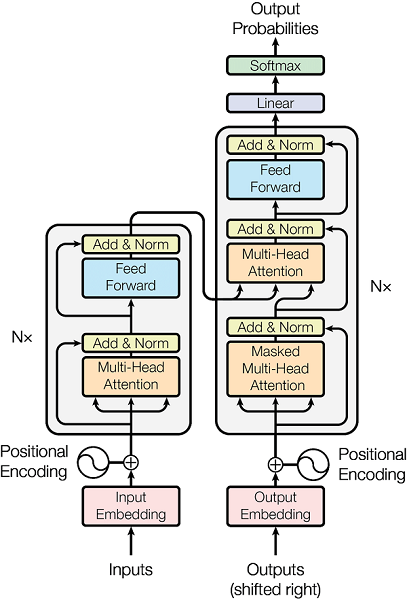
\includegraphics[width=9cm]{img/transformer.png}

  \caption{The overall schema of the Transformer model. Inputs are summed with
    positional encodings. Encoder processes the input in $N$ stack layers. Each
    encoder layer consists of self-attention and feed-forward sub-layer. Layers
    are interconnected with residual connections and layer normalization is
    applied on the output of each layer. The decoder stack uses three
    sub-layers, where the additional cross-attention layer attends to the
    encoder output. We show the original image from
    \citet{vaswani2017attention}.}
  \label{fig:transformer}
\end{figure}

% - - - - - - - - - - - - - - - - - - - - - - - - - - - - - - - - - - - - - - -
\paragraph{Positional Encoding.} Since the self attention is a commutative
operation, the ordering of the input tokens needs to be modeled explicitly.
The standard technique is to use sinusoidal encodings, proposed in the original
paper. Positional encoding is a vector of the same dimension as the word
embedding which is computed using the position of the word on the input.
The $2i$-th and $(2i+1)$-th elements of the positional encoding of word on
position $j$ is computed as follows:
%
\begin{equation}
  \begin{split}
    E_{\text{pos}}(j, 2i) &= \sin(j / 10000^{2i/d}) \\
    E_{\text{pos}}(j, 2i + 1) &= \cos(j / 10000^{2i/d})
  \end{split}
\end{equation}
%
where $d$ is the \emph{model dimension}. This number is equal to the dimension
of the word embeddings. Before an input word $w_i$ is processed by the network,
the positional encodings are added to the word embeddings:
\begin{equation}
  E(w_i) = E(w) + E_{\text{pos}}(i)
\end{equation}

% - - - - - - - - - - - - - - - - - - - - - - - - - - - - - - - - - - - - - - -
\paragraph{Self-Attention.} The key component of the Transformer model is the
self-attention. As the name suggests, self-attention is run with the same set
of states used as both queries, keys, and values. Scaled dot-product is used as
the similarity metric, so the attention itself does not use any trainable
parameters. Formally, self-attention is defined as function:
%
\begin{equation}
  \mathcal{A}(Q,K,V) = \softmax \left( \frac{QK^\top}{\sqrt{d}} V  \right)
  \label{eq:scaled-dot-product}
\end{equation}
%
where the values $Q, K, V \in \mathbb{R}^{T \times d}$ ($T$ being the sequence
length) are computed from the same input, usually using a linear projection.

Self-attention sub-layers are used both in the encoder and the decoder. Because
the decoder is autoregressive, the self-attention module needs to be
constrained to attend only to the preceding states (so the model does not
``glance into the future''). This is implemented by applying a triangular mask
on the attention query and key matrix, hence the name \emph{masked
  self-attetnion}.

% - - - - - - - - - - - - - - - - - - - - - - - - - - - - - - - - - - - - - - -
\paragraph{Multi-Head Attention.} Instead of running a single self-attention
per layer, the model structure is enriched by splitting the self-attention into
multiple \emph{heads}. First, each state is projected into $h$ triples of
queries, keys, and values. Then, self-attention is computed on each triple.
Finally, the self attention outputs are mixed together into a single output
sequence:
%
\begin{equation}
  \mathcal{A}^h(Q, K, V) = \sum_{i=1}^h C_i W_i^O \\
\end{equation}
%
where $W_i^O \in \mathbb{R}^{d_h \times d}$ is a parameter matrix used for
projecting the outputs from the individual attention heads into a single
output, and
%
\begin{equation}
  C_i = \mathcal{A}(QW_i^Q, KW_i^K, VW_i^V)
\end{equation}
where $W_i^Q, W_i^K, W_i^V \in \mathbb{R}^{d \times d_h}$ are trainable
matrices that project the states to inputs for the $i$-th attention head
(defined in Equation \ref{eq:scaled-dot-product}). In self-attention,
$Q = K = V \in \mathbb{R}^{T \times d}$ is the set of $T$ states of the current
layer.

% - - - - - - - - - - - - - - - - - - - - - - - - - - - - - - - - - - - - - - -
\paragraph{Cross-Attention.} Each layer in Transformer encoder consists of a
self-attention and a feed-forward sub-layer. The decoder inserts an
\emph{encoder-decoder attetnion}, or \emph{cross-attention} layer.  The
cross-attention layer functions exactly like self-attention layer, but the
queries $Q$ are the decoder states (i.e. the output of the preceding
self-attention), and the keys and values $K = V$ correspond to the encoder
output states.

% - - - - - - - - - - - - - - - - - - - - - - - - - - - - - - - - - - - - - - -
\paragraph{Feed-Forward Layer.} Each Transformer layer consists
of self-attention, optionally a cross-attention, followed by a feed-forward
network. This feed-forward network uses the same parameters for all positions
along the state sequence. The network takes a state $x$ and feeds it through a
single hidden layer with a ReLU activation:

\begin{equation}
  \mathcal{F}(x) = \max(0, W_1^Fx + b_1^F)W_2^F + b_2^F
\end{equation}
where $W_1^F \in \mathbb{R}^{d \times d_f}$, $b_1 \in \mathbb{R}^{d_f}$,
$W_2^F \in \mathbb{R}^{d_f \times d}$, and $b_2^F \in \mathbb{R}^d$ are the
weight and bias parameters of the feed-forward network $\mathcal{F}$, and $d_f$
is the dimension of the hidden state.

% - - - - - - - - - - - - - - - - - - - - - - - - - - - - - - - - - - - - - - -
\paragraph{Residual Connections and Layer Normalization.} As a post-processing
step, the output of each sub-layer is connected with the output of the previous
sub-layer with residual connections. \JH{zkontrolovat jestli se to definovalo v
  Deep Architectures, stejně jako Layer Norm.} Similarly to the
\glsentryshort{rnn}-based deep architectures, layer normalization is used in
combination, which ties all states in the sub-layer stack into a shared vector
space.

% - - - - - - - - - - - - - - - - - - - - - - - - - - - - - - - - - - - - - - -
\paragraph{Model Hyperparameters.} The parameters that control the model size
are the model dimension $d$, the number of attention heads $h$, the dimension
of the feed-forward hidden layer $d_f$, and the number of Transformer layers in
the encoder and decoder stack. Note that the dimension of keys and values in a
single attention head $d_h$ is commonly set to be $d / h$, but can be
customized as well.  As a regularization, dropout \citep{srivastava2014dropout}
is applied with rate $P_d$ to the output of each sub-layer before
normalization.

The authors of the architecture propose two presets for these parameters, named
\emph{base} and \emph{big}. Table~\ref{tab:transformer-hyperparams} shows the
hyperparameter values for these two settings.

\begin{table}
  \centering
  \begin{tabular}{lrrrrrr}
    \toprule
      & \# of layers &  $d$  &  $h$  & $d_h$ & $d_f$ & $P_d$ \\
    \midrule
    Transformer base  & 6 &  512  & 8 & 64 &  2,048 & 0.1 \\
    Transformer big  & 6 &  1,024  & 16 & 64 &  4,096 & 0.3 \\
    \bottomrule
  \end{tabular}
  \caption{The hyperparameter values for Transformer base and big variants.}%
  \label{tab:transformer-hyperparams}
\end{table}


% ------------------------------------------------------------------------------
\section{Training}
\label{sec:training}
% ------------------------------------------------------------------------------

Training of \gls{nmt} models is usually done under \emph{supervised}
conditions, using a dataset of parallel sentences. \JH{move the following to
  the experimental section:} The size of the available data varies a lot with
different language pairs. Although there is no formal definition, when there is
less than a million sentence pairs available, the language pair is reffered to
as being \emph{low-resource}. For many languages, even a million sentences is a
very large number compared to what is actually available. The data quality is
also a factor. For example, when the only available data is crawled from the
web, data cleaning can filter out a major part of the corpus. In this thesis,
we focus on language pairs where the data size is not a major issue and we
simulate the low-resource scenario using Romanian-English translation.

Translation models are trained by minimizing the loss function, usually
expressed by cross-entropy between the output distribution and the one-hot
distribution which assigns the probability of one to the correct target word,
and zero probabilities to the other words. Assuming $y_i$ is the correct target
word at position $i$, $p_{\text{ref}}$ is the one-hot distribution, and $p$ is
the distribution predicted by the model, we have:
%
\begin{equation}
  \begin{split}
    H(p_{\text{ref}}, p) &=  - \sum_{w \in \mathcal{V}} p_{\text{ref}}(w) \log p(w) = \\
    &=  - \log p(y_i)
  \end{split}
\end{equation}
%
where $\mathcal{V}$ is the vocabulary. Note that in autoregressive models, the
output distributions $p$ and $p_{\text{ref}}$ are conditioned on the preceding
target words.

Given model parameters $\theta$, the word-level cross-entropy is summed across
the sentence pairs in the data $D$ to obtain the negative log likelihood of the
dataset $J_{\theta}$:
%
\begin{equation}
  \begin{split}
  J_{\theta} &= - \sum_{(x, y) \in D} \sum_{i = 1}^{T_y} \log p(y_i | x, y_{<i}, \theta) \\
  &= - \sum_{(x, y) \in D} \log p(y | x, \theta)
  \end{split} \label{eq:loss}
\end{equation}
%
where $y_{<i}$ denote the target prefix and $T_{y}$ is the length of the target
sentence $y$. The probability of a sentence can be reformulated using the chain
rule.
\JH{rovnice J hvězdička = argmin J over thetas}

% Since the probability distributions are conditioned on the previously decoded
% tokens, the likelihood of the target sentence is reformulated using the chain
% rule:
% %
% \begin{equation}
%   J_{\theta} = - \sum_{(x, y) \in D} \sum_{i = 1}^{T_y} \log p(y_i | x, y_{<i}, \theta)
% \end{equation}
% %
% where $T_y$ is the length of the target sentence.



% - - - - - - - - - - - - - - - - - - - - - - - - - - - - - - - - - - - - - - -
\paragraph{Teacher Forcing.}
Note that in the equations above, the probability distributions are conditioned
on the reference target prefix, rather than the model outputs. This technique
is known as \emph{teacher forcing}, and is essential for the training
convergence. When the model is exposed to its own outputs from the start of the
training, it will very likely fail to converge.

Teacher forcing, however, brings along a problem called \emph{exposure bias} --
the model is never exposed to its own errors, which makes it less robust
against them.

Methods have been proposed to address this issue, including a curriculum
learning approach which gradually replaces teacher forcing with the model
predictions \citep{bengio2015scheduled}. Other methods focus on sequence-level
training or beam search optimization methods, mostly based on reinforcement
learning \citep{williams1992simple, wiseman-rush-2016-sequence,
  ranzato2016sequence}. However, none of these methods was widely adopted, and
current models are believed to be capable of recover from their errors despite
being explicitly trained to do so.

% - - - - - - - - - - - - - - - - - - - - - - - - - - - - - - - - - - - - - - -
%\paragraph{RNNs vs Transformer Training.} A significant difference in training
%\glspl{rnn} and the Transformer model is

% - - - - - - - - - - - - - - - - - - - - - - - - - - - - - - - - - - - - - - -
\subsection{Training Methodology}
\label{sec:training:methodology}
% - - - - - - - - - - - - - - - - - - - - - - - - - - - - - - - - - - - - - - -

In this section, we go through the common techniques for successful training of
\gls{nmt} models. These include data cleaning and augmentation methods,
optimization settings, and hardware considerations.

% - - - - - - - - - - - - - - - - - - - - - - - - - - - - - - - - - - - - - - -
\paragraph{Data Cleaning.} With a few exceptions for high-resource languages,
the training data are usually acquired from the Web. Depending on the data
source and the extraction technique, there is a level of noise present in the
data. In many cases, it is necessary to consider data cleaning before training
any models.

The basic data cleaning techniques are rule-based and include language
identification, and filtering sentence pairs with odd characters or length
ratios. Deduplication may be considered, but might be harmful when it removes
short sentences which appear commonly in the given language. For example, if
English sentences ``Thank you'' and ``Thank you xxx'' both appear in the data
as translations of the Czech ``Děkuji'', they might get equal probabilities
when deduplication is used. Without deduplication, the frequency of the correct
translation would be much higher in the training data.

An advanced data cleaning technique is dual conditional cross-entropy filtering
\citep{junczys-dowmunt-2018-dual}. Using two translation models trained on
clean data in opposite directions, each sentence pair is scored according to
the cross entropies assigned by the translation models to the sentence
pair. When the cross entropies differ, or when both cross entropy scores are
high, the score is low. When the cross entropies are similar and are low, the
score is high. After scoring, low-scoring sentence pairs are removed from the
data using an empirically set threshold.

% - - - - - - - - - - - - - - - - - - - - - - - - - - - - - - - - - - - - - - -
\paragraph{Data Augmentation.} The size of the training data is a key factor to
model performance. In rare cases of high-resource languages, there is enough
parallel data available to train a decent translation model. But even for these
languages, data augmentation methods, namely \emph{backtranslation} are used
to create bigger data and therefore to improve the model performance.

Backtranslation is a simple technique for incorporating target-side monolingual
data in a \gls{nmt} model \citep{sennrich-etal-2016-improving}. For a given
translation direction, we first translate the monolingual data from the target
language to the source language using a previously trained model. Then, we mix
the synthetic source-language data along with the authentic target-language
data into our training corpus. When the parallel-to-monolingual data size ratio
not balanced, one can consider oversampling the smaller part of the corpus to
mitigate this. Recently, \citet{caswell-etal-2019-tagged} showed that labeling
the synthetic data with a special token improves the translation quality. As
pointed out by \citet{marie-etal-2020-tagged}, this helps because the model is
less prone to overfitting to this type of data.

\emph{Knowledge distillation} \citep{kim-rush-2016-sequence} is another data
augmentation technique. Unlike backtranslation, knowledge distillation is used
mainly for improving the model efficiency, both in terms of memory and speed.
Also unlike backtranslation, we use target-language synthetic data. In the
simplest setting, we use a well-trained and large \emph{teacher} model to
translate its own training data. Then, we train a smaller (and therefore faster
and smaller) \emph{student} model on the outputs of the teacher model. This
technique shows that for a small sacrifice of the translation quality, we can
get interesting improvements in terms of speed, which is useful for deploying
the models in a limited environment, such as a mobile device.

% - - - - - - - - - - - - - - - - - - - - - - - - - - - - - - - - - - - - - - -
\paragraph{Batching.} In Equation \ref{eq:loss}, the loss function
$\mathcal{J_\theta}$ is defined as a sum of sequence-level losses over dataset
$D$. We use gradient descent to find parameters $\theta$ which minimize the
loss value. However, the exact computation of the gradient is inefficient
because it requires one pass through the whole dataset. Therefore, we estimate
the gradient on a small sample of the training data, called a \emph{mini
  batch}, or simply a batch. This method is called \emph{stochastic gradient
  descent}.

The size of a mini batch is an important parameter and its value can have a
large impact on the training convergence. Bigger batches provide better
gradient estimates, but require more memory, which is an issue when using a
GPU.

\JH{shuffling goes here}

\JH{optimizer delay perhaps also here}

% - - - - - - - - - - - - - - - - - - - - - - - - - - - - - - - - - - - - - - -
\paragraph{Optimization.}


% - - - - - - - - - - - - - - - - - - - - - - - - - - - - - - - - - - - - - - -
\paragraph{Parameter Initialization.}

\JH{random initialization vs pretraining / transfer learning}


% - - - - - - - - - - - - - - - - - - - - - - - - - - - - - - - - - - - - - - -
\paragraph{Early Stopping.} To avoid overfitting, the model should be regularly
tested on a validation dataset over the course of the training. The validation
data should not overlap with the training or test data. Once the model stops
improving on a chosen validation metric, the training process is
interrupted. This method is reffered to as \emph{early stopping}. Usually, the
validation metric is either the cross-entropy loss, or the target evaluation
metric, such as BLEU. An alternative early stopping method is to save the
parameters of the best performing model on validation.

% - - - - - - - - - - - - - - - - - - - - - - - - - - - - - - - - - - - - - - -
\paragraph{Hardware.}




% ------------------------------------------------------------------------------
\section{Autoregressive Decoding}
\label{sec:training-vs-inference}
% ------------------------------------------------------------------------------

The models we described in the sections above are \emph{autoregressive} -- the
output tokens are predicted left-to-right, while every decision is conditioned
on the previously generated outputs. With this property, there comes an
important distinction in behavior between training and decoding. Whereas during
training, the ground-truth data are used to simulate the previous decisions,
during decoding, the ground truth is unknown and therefore the model needs to
rely solely on its own decisions. This constitutes a theoretical problem,
called \emph{exposure bias} -- the model is never exposed to its own errors
during training.

In the RNN-based models, the difference between training and decoding is
minimal. The model execution is done the same way, with the one exception of
providing ground-truth data during training. Another exception is that the final
softmax does not need to be computed during greedy decoding (there is no need
for normalized distribution if we are interested only in the token with maximum
probability), but is still needed for beam search.

The Transformer models are quite different in this aspect. Since there is no
recurrence operation which requires accumulation of information in a hidden
state, the network can be trained on a whole ground-truth sentence in one step.
The only requirement is to prevent the decoder self-attention from attending to
the future positions. However, during training, the model is still conditioned
on its own decisions. \JH{tohle neni pravda}




\section{Evaluation}
\label{sec:evaluation}

The problem of \gls{mt} evaluation is almost as challenging as \gls{mt} itself.
The most reliable method for assessing the quality of \gls{mt} systems remains
human evaluation.  Since the adoption of statistical approach for \gls{mt}
\citep{brown-etal-1993-mathematics,koehn-etal-2003-statistical}, the demand for
automatic translation quality metrics grew larger, as the models often need to
be validated several times during training.

Perhaps the best-known automatic \gls{mt} metric is BLEU
\citep{papineni2002bleu}.  Despite a long term effort led by the organizers of
the WMT Metrics shared task to create an automatic evaluation metric that would
be better correlated with scores assigned by humans, BLEU continues to be the
most widely used metric in the contemporary literature. However, over the nearly
two decades of using BLEU, it has been criticized for being prone to errors due
to outliers or being too inaccurate when the score itself is low.
\citep{callison-burch-etal-2006-evaluating,bojar-etal-2010-tackling,reiter2018structured,mathur-etal-2020-tangled}

\JH{evaluation of decoding speed -- latency, throughput}



%%% Local Variables:
%%% mode: latex
%%% TeX-master: "thesis"
%%% End:

% %%%%%%%%%%%%%%%%%%%%%%%%%%%%%%%%%%%%%%%%%%%%%%%%%%%%%%%%%%%%%%%%%%%%%%%%%%%%%
\chapter{Non-Autoregressive NMT}
\label{chap:nat}
% %%%%%%%%%%%%%%%%%%%%%%%%%%%%%%%%%%%%%%%%%%%%%%%%%%%%%%%%%%%%%%%%%%%%%%%%%%%%%

In real-world applications of \ac{mt}, efficiency is often crucial.  Most
commercial \ac{nmt} models are available through a cloud-based service, such as
Microsoft Translator\footnote{\url{https://microsoft.com/translator/}} or
Google Translate.\footnote{\url{https://translate.google.com/}} Scaling
cloud-based solutions for large user bases is simple but costly. Even with a
large pool of computational resources, it is worthwhile to implement
optimizations which decrease model latency and improve user experience.

Locally deployed \ac{nmt} models provide a number of advantages over
cloud-based solutions. First, the service does not rely on internet
connection. Second, the data is not being sent to a third party server, and
therefore it is suitable for translating private or confidential data.
However, without optimization, running state-of-the-art translation models
locally often requires specialized hardware, such as one or more
GPUs. Otherwise, the time to translate a single sentence can easily exceed one
second on a standard CPU.

Higher decoding speeds can be achieved by model optimization. In their 2019
submission to the \ac{wngt} Efficiency Shared Task,
\citet{kim-etal-2019-research} successfully employed knowledge distillation,
quantization, shortlisting \citep{jean-etal-2015-using} and a simpler recurrent
unit design to bring the throughput of a translation model up to 3,600 words
per second on a CPU, with a modest drop in the translation quality. Following
this work, \citet{bogoychev-etal-2020-edinburghs} reported further improvements
with attention head pruning \citep{voita-etal-2019-analyzing}. Their work has
been a part of the Bergamot research project, which aims to bring offline
translation models into a browser.\footnote{\url{https://browser.mt/}}

\Ac{nar} models present an alternative approach to model optimization, using
different architecture and a different decoding algorithm which has lower time
complexity.  In \ac{nmt}, a non-autoregressive decoding algorithm does not
access previously decoded outputs, imposing conditional independence
assumption on the output token probability distributions. This assumption
allows to parallelize of the decoding, which can significantly reduce the
latency of the translation system. On the other hand, it also presents a
challenge to the language model, which usually leads to poorer translation
quality.

The research presented in this thesis is focused on the usefulness of \ac{nar}
models for translation (\acs{nat}\glsunset{nat}) in the quest for faster
translation models. We first analyze the \ac{nat} models alone and assess the
necessary techniques needed to match the quality of \ac{ar} models.  Then, we
adapt the optimizations successfully used in \ac{ar} models for \ac{nar} models
and evaluate the additional speed gains. \JH{This is currently not in the
  thesis. We'll have shortlisting with a fast implementation. Add reference to
  Chapter \ref{chap:experiments} when ready.}

In this chapter, we present an overview of the current state of the research
and the key concepts in non-autoregressive \ac{nmt}. We begin with the
description of the general, commonly used principles of \ac{nat} in Section
\ref{sec:nat:principles}. Then, we provide a survey of notable approaches to
\ac{nat}, focusing on extensions to the basic models that improve output
quality. We categorize them into four groups, each of which is described in
separate section: First, the methods based on relaxing the alignment between
the output and target sequences, which are most similar to our work in Chapters
\ref{chap:nar-nmt-ctc} and \ref{chap:experiments}, are described in Section
\ref{sec:nat:alignment}. Methods that improve the training process using
auxiliary objectives are described in Section \ref{sec:nat:aux}. Section
\ref{sec:nat:semi} introduces approaches based on iterative decoding. Relevant
methods not falling clearly into any of the categories above are summarized in
Section \ref{sec:nat:misc}. Natually, the groups are not mutually exclusive and
there is an overlap. We conclude this chapter with a discussion of the
limitations of the presented literature, mostly concerning the evaluation
methodology.


% ------------------------------------------------------------------------------
\section{Non-Autoregressive Models}%
\label{sec:nat:principles}
% ------------------------------------------------------------------------------

This section summarizes the main features of \ac{nar} models, some of the basic
concepts and research problems in this field. The \ac{nar} variant of the
Transformer model was first described by \citet{gu2017nonautoregressive} and
\citet{lee-etal-2018-deterministic}. Each of these two foundational papers
provides different (complementary) grounds for further research discussed later
in this chapter -- latent variables, and iterative decoding.

% ------------------------------------------------------------------------------
\paragraph{Conditional Independence.} The defining feature of a
non-autoregressive model is the assumption of conditional independence between
the output distributions across time steps. Recall Equation
\ref{eq:output-distribution}, which defines the output distribution for
autoregressive models:
%
\begin{equation*}
  p(y|x) = \prod_{t=1}^{T_y}p(y_t|y_{<t},x,\theta)
  \tag{\ref{eq:output-distribution}}
\end{equation*}
%
Unlike Equation \ref{eq:output-distribution}, \Ac{nat} models do not condition
the output token probabilities on previously decoded outputs $y_{<t}$.  The
probability of an output sentence $y$ given an input sequence $x$ can then be
modeled as:
%
\begin{equation}
  p(y|x) = \prod_{t=1}^{T_y}p(y_t|x,\theta)
  \label{eq:nat-output-distribution}
\end{equation}

Although technically possible, making the outputs in \acs{rnn}-based models
conditionally independent does not reduce the time complexity because in
\acsp{rnn}, the value of each hidden state depends on the value of the
preceding state (see Section \ref{sec:encdec:rnn}). However, in the Transformer
model (see Section \ref{sec:encdec:transformer}), hidden states in each layer
depend only on the states from the previous layer. This allows for parallel
computation on the level of layers.

In the following paragraphs, we discuss the necessary alterations to the
Transformer architecture. Since the outputs are conditionally independent, we
cannot feed the previously decoded outputs into the Transformer decoder. We
need to provide the decoder inputs and estimate the target length. The causal
mask over decoder self-attention is now unnecessary. We also address the main
issue and the reason \ac{ar} models are still superior in modeling language.

% ------------------------------------------------------------------------------
\paragraph{Multimodality Problem.} In one of the first applications of a
non-autoregressive model to \ac{nmt}, \citet{gu2017nonautoregressive} describe
the \emph{multimodality problem} which arises when the outputs are
conditionally independent.

When estimating the probability of a word on a given position, there may be
multiple words which get a high probability. These words are the so called
\emph{modes} of the distribution. In autoregressive models, once a word gets
selected, other modes are ignored in the following time steps. However, a
non-autoregressive model does not base its decision for a given position on the
preceding ones, so when multiple positions have multiple modes, the model has
no means of coordinating the selection of modes across different time steps.

% This issue is illustrated in Figure \ref{fig:multimodality-problem}.
% \begin{figure}
%   \centering
%   \begin{minipage}{\textwidth}
%     source: thank you

%     \begin{center}
%     \begin{tabular}{cccc}
%       \toprule
%       $y_1$ & $p(y_1|x)$ & $y_2$ & $p(y_2|x)$ \\
%       \midrule
%       vielen & 0.4 & dank & 0.4 \\
%       danke  & 0.3 & schön & 0.3 \\
%       \vdots & & \vdots & & \\
%       \bottomrule
%     \end{tabular}
%     \end{center}

%   \end{minipage}
%   \caption{Illustration of the multimodality problem.}
%   \label{fig:multimodality-problem}
% \end{figure}

A well-known example of the multimodality problem is the translation of the
sentence ``thank you'' into German, which has two equally likely translations:
``vielen dank'' and ``danke schön.'' In this case, the pair of German tokens
``danke'' and ``vielen'' create the two modes on the first position, and the
tokens ``dank'' and ``schön'' are the modes on the second position. If an
\acl{ar} model chooses to generate ``danke'' on the first position, the token
``dank'' on the second position will no longer receive high probability by the
model. However, when a \acl{nar} model assigns high probabilities to the
correct translations, it also has to assign high probabilities to the other
(incorrect) two combinations, ``danke dank'' and ``vielen schön''
\citep{gu2017nonautoregressive}.

% ------------------------------------------------------------------------------
\paragraph{Target Length Estimation.} In a standard \ac{ar} \ac{nmt} model such
as the Transformer or an \acs{rnn}-based model with attention, the length of
the output sentence is modeled implicitly by using the special end-of-sentence
(\eos{}) token. Equations \ref{eq:output-distribution} and
\ref{eq:nat-output-distribution} work with the sentence length implicitly,
assuming that the last token $y_{T_y}$ is the \eos{} token and that \eos{} does
not appear among the previous tokens $y_{<T_y}$.

The probability distribution in Equation \ref{eq:nat-output-distribution} can
be factorized to express the estimation of the target sentence length
explicitly: %leaving out the \eos{} symbol from the mathematical model:
\begin{equation}
  p(y|x, \theta) = p_L(T_y|x, \theta) \cdot \prod_{t=1}^{T_y}p(y_t|x,\theta).
  \label{eq:explicit-length}
\end{equation}

The explicit target length estimation is a useful technique of moderating the
multimodality problem. \JH{Clarify how.} It also helps with the problem of
supplying inputs for the decoder.

% ------------------------------------------------------------------------------
\paragraph{Decoder Inputs.} A \acs{nar} Transformer decoder cannot
receive the previously decoded tokens on the input. A solution proposed by
\citet{gu2017nonautoregressive} is to use a simple fertility model, which also
serves as the explicit target length estimator.

Compared to the autoregressive Transformer model, the model has the following
modifications. First, the inputs to the decoder are made up of the sequence of
encoder inputs, either uniformly stretched to the predicted target sentence
length, or copied using a fertility model. Second, the decoder self-attention
does not use the causal mask since all states can now attend to all other
states in both directions. Third, \emph{positional attention} is added to every
decoder layer, where the positional encoding is used as queries and keys and
the decoder states as values. \JH{Explain.}

In \citet{gu2017nonautoregressive}, the multimodality problem (and the length
estimation) is addressed by introducing latent fertility variables
$F = f_1, \ldots, f_{T_x}$ sampled from a prior distribution. Each
$f_i \in \mathbb{N}_0$ denotes the number of times to copy $x_i$ to the decoder
input (summing up to the target length $T_y$). The output probability is then
conditioned on the latent vector $F$, which is marginalized out:
%
\begin{equation}
  p(y|x, \theta) = \sum_{F \in \mathcal{F}} p(F|x, \theta) \cdot p(y|x, F, \theta)
\end{equation}
%
where the fertility model $p(F|x, \theta)$ and the translation model
$p(y|x, F, \theta)$ can be trained jointly using a variational lower bound with
a candidate distribution $q$:
\begin{align}
  \begin{split}
    \mathcal{L}(\theta)
    & = \log p(y|x, \theta) = \log \sum_{F \in \mathcal{F}} p(F| x, \theta ) \cdot p(y | x, F, \theta) \\
    & \geq \mathbb{E}_{F \sim q} \left(\sum_{t=1}^{T_y} \log p(y_t | x, F, \theta)
      + \sum_{t=1}^{T_x} \log p(f_t | x, \theta) \right) + \mathcal{H}(q)
  \end{split}
\end{align}
%
where $q$ is an external deterministic fertility model, and therefore
$\mathcal{H}$ is a constant and the expectation is also deterministic. \JH{I
  dont completely understand but assume that there is a single sample with
  probability of 1, so you just minimize the inside of the big bracket and
  ignore the rest.}
%
The fertility model depends on an external module which is not trained together
with the model. The authors fine-tune the trained translation model using
reinforcement learning \citep{williams1992simple} to estimate the gradients of
the fertility model.

During decoding, marginalizing over all possible fertility values is
intractable. Therefore, \citet{gu2017nonautoregressive} experiment with three
approximation methods -- argmax, average decoding, and \ac{npd}. \JH{Explain
  the three methods, diff to LPD} \JH{There is another comment in the PDF.}

% ------------------------------------------------------------------------------
\paragraph{Autoregressive Rescoring.} A usual technique in the \ac{nat}
literature is to use some form of rescoring of the outputs of the \acl{nar}
model by an \acl{ar} model. The nature of the Transformer model allows to score
a sentence in a single step (as opposed to generating one), which means that
the additional rescoring computation increases the decoding complexity only
linearly with respect to the number of the candidates for rescoring.

The choice of the rescoring candidates varies. \citet{gu2017nonautoregressive}
use \ac{npd} which first samples the decoder input sequences from the fertility
distribution, computes the best candidate for each input, and then rescores the
results using an \ac{ar} model. A closely related method is \ac{lpd} which
generates and scores sentences of different lengths.

Note that in contrast to \ac{ar} models, the highest-scoring sequence in an
\acs{nar} model can be found simply by taking the highest-scoring token in each
step, because of the conditional independence assumption.

% ------------------------------------------------------------------------------
\paragraph{Knowledge Distillation.} To tackle the multimodality problem from
another angle, \citet{gu2017nonautoregressive} propose to use sequence-level
knowledge distillation to create artificial training data
\citep{kim-rush-2016-sequence}. \JH{One or two sentences of what is happening
  here.} The main idea is that outputs of a teacher model will have a simpler
structure than natural language, limiting the number of the distribution modes.

According to an ablation study published by \citet{gu-kong-2021-fully}, using
knowledge distillation is a crucial element in training non-autoregressive
translation models, regardless the actual method used.
\citet{zhou-etal-2020-understanding} further study the effects of knowledge
distillation strategies on the translation quality of \ac{nar} models. \JH{One
  sentence to summarize their main finding.}

% ------------------------------------------------------------------------------
\paragraph{Iterative Refinement.} Modeling fertility introduces latent
variables into a \acl{nar} model. A different approach was proposed by
\citet{lee-etal-2018-deterministic}. Instead of modeling fertility, the authors
introduce $L$ discrete sequential latent variables interpreted as stages of
refinement:
%
\begin{align}
  \begin{split}
    p(y|x) & = \sum_{y^L}
      \left( \prod_{t=1}^{T_y} p(y_t|y^L, x) \right) p(y^L|x) \\
    p(y^L|x) & = \sum_{y^{L-1}}
      \left( \prod_{t=1}^{T_y} p(y_t^L | y^{L-1}, x) \right)
      p(y^{L-1}|x) \\
    \vdots \\
    p(y^0|x) & = \prod_{t=1}^{T_y} p(y_t^0|x)
  \end{split}
\end{align}
%
Each summation in the equations above is computed over the whole space of
possible sequences, and thus, it is intractable to calculate the probablility
$p(y|x)$ exactly. To overcome this problem, the authors approximate the sums
with only the element corresponding to the sequence with the largest
probability, $\hat{y} = \argmax_{y}p(y|x)$. Putting it together with the
equations above and moving to the logarithmic domain, we get:
\begin{align}
  \begin{split}
    \log p(y|x) \geq
    & \sum_{t=1}^{T_y} \log p(y_t| \hat{y}^L, x) + \\
    & + \sum_{t=1}^{T_y} \log p(\hat{y}_t^{L}| \hat{y}^{L-1}, x) + \ldots \\
    & + \sum_{t=1}^{T_y} \log p(\hat{y}_t^0 | x). \label{eq:refinement-lowerbound}
    % = & \sum_{l=0}^{L} \sum_{t=1}^{T_Y} \log p(\hat{y}_t^{l+1} | \hat{Y}^l, X)
  \end{split}
\end{align}
%where $Y^0 = X$ and $\hat{y}_t^{L+1} = y_t$.

The tokens $\hat{y}_t^0$ in the initial sequence are set to $x_{t'}$ where
$t' = (T_x / T_y) \cdot t$, i.e. the source sentence is either squished or
stretched by copying or omitting some of the source words in order to fit the
target sentence length. During training, the length of the reference sentence
is known. During decoding, the authors use a separate model $p(T_y|x)$ for
target length prediction. All probability distributions in the above equations
are modeled with neural networks with shared parameters. In this way, the
number of intermediate refinement steps during decoding can be chosen
arbitrarily and remains flexible after the model is trained.

The latent variable model is trained by minimizing the log-likelihood of the
reference sentence $y^*$ in each of the refinement steps:
\begin{equation}
  \mathcal{L}_{\text{LVM}}(\theta) = - \sum_{l=1}^{L+1} \left(
    \sum_{t=1}^{T_{y^*}} \log p(y_t^* | \hat{y}^{l-1}, x, \theta)
  \right) \label{eq:refinement-lvm-loss}
\end{equation}

\citet{lee-etal-2018-deterministic} also discuss the training of the refinement
process from a non-iterative denoising perspective. Formally, they introduce an
additional denoising autoencoder loss to the model:
%
\begin{equation}
  \mathcal{L}_{\text{DAE}}(\theta) = - \sum_{t=1}^{T_y} \log p(y_t^* | \bar{y}, x, \theta)
\end{equation}
where $\bar{y}$ is a corrupted version of the reference translation $y^*$. The
corruption process is performed on each token with a probability $\beta$. Each
corrupted token is either replaced with a random word from the vocabulary,
copied to its neighbor, or swapped with the neighbor.

During training, the two loss functions are stochastically mixed using a
hyperparameter $\alpha$, sampled from a Bernoulli distribution. In other words,
in each refinement step, the input to the decoder is either the output of the
previous refinement step, or a corrupted version of the reference sentence.

% ------------------------------------------------------------------------------
\section{Alignment-Based Methods}%
\label{sec:nat:alignment}
% ------------------------------------------------------------------------------

\Acl{ar} models are trained using the cross-entropy loss (recall Equation
\ref{eq:loss} in Section \ref{sec:training}). If we assume a single sentence
pair $(x,y)$, the negative log-likelihood is the sum of negative
log-probabilities $\log p(y_i|x, y_{<i}, \theta)$ for $i=1, \ldots, T_y$, as
estimated by the model with parameters $\theta$.  Notice how the ground-truth
sequence $y_1, \ldots, y_{T_y}$ corresponds to the sequence of the
probabilities $p(y_i|\ldots)$: we require that the $i$-th reference token is
decoded at the $i$-th position of the output state sequence. The methods
described in this section relax this requirement.

We define alignment as a function $a$ which maps the positions in the
ground-truth sentence to the positions in the output. In autoregressive models,
$a(i) = i$ for every position $i$ in the ground truth. % When we
% generalize the cross-entropy loss for sentence pair $(x, y)$ to account for the
% alignment, we get
Methods that consider different alignments allow working with output and label
sequences of different lengths, which is a useful feature in the context of
\ac{nat} models.

To the best of our knowledge, we were the first to propose an alignment-based
method for \ac{nat} \citep{libovicky-helcl-2018-end}. Our method is based on
\acf{ctc}\glsunset{ctc}, which computes the cross-entropy losses over all
possible alignments between the ground truth and a longer output state
sequence. We describe this method in detail in Chapter \ref{chap:nar-nmt-ctc}.
In the following paragraphs, we present a number of related methods based on
modeling the alignment between the sequences of outputs and ground-truth
labels.

% -----------------------------------------------------------------------------
\paragraph{Aligned Cross Entropy for \ac{nat}.} The main problem with using
cross-entropy objective for training \ac{nat} models is that it heavily
penalizes misaligned target words. If a correct word is generated at an
incorrect position in the target sentence, it does not have a positive effect
on the loss, same as if a completely unrelated word is generated. In \acl{ar}
models, this problem is avoided with teacher forcing -- the model is provided
with the preceding words from the reference sentence. Without teacher forcing,
the alignment between the predicted distributions and the positions in the
reference sentence is too rigid. For example, consider the reference sentence
``Thank you for your cooperation.'' In a \acl{nar} model, another valid
translation ``Thanks for your cooperation'' receives the same training signal
as a completely wrong translation. The crucial difference in \ac{ar} models is
that to train prediction at the second position, the target word ``Thank'' for
the first position is provided on the input, so the word ``for'' does not
receive high probability.

One way to address this problem is to consider the alignment as a latent
variable.  The \acl{axe} \glsunset{axe} (\acs{axe};
\citealp{ghazvininejad2020aligned}) objective function uses a dynamic
programming algorithm to find the alignment with the minimum cross-entropy
loss. In the example from the previous paragraph, the alignment with the lowest
cross-entropy is the one that aligns the positions 3--5 from the label sequence
(representing the suffix ``for your cooperation'') to output positions 2--4 in
the output. Either of the first two positions in the label sequence can be
aligned to the first position in the output sequence, while the other label
position remains unaligned. \JH{obrazek?}

The alignments considered in the \ac{axe} approach are monotonic (i.e.
$a(i) \leq a(j)$ for every $i \leq j$, when defined), but the mapping does not
have to be defined for each ground-truth position. Similarly, not all positions
in the prediciton sequence are not required to be mapped to a reference
position.  In case of skipping a prediction, the model learns to output an
empty token $\epsilon$, i.e. $-\log p(y_t = \epsilon | x, \theta)$ is added to
the loss.  When a position in the ground-truth sequence is skipped, the
negative log-probability of the skipped token is added to the loss at the
current prediction position, weighted by a hyperparameter $\delta$ which
controls the cost of the skip-target operation. An example of such alignment is
shown in Figure \ref{fig:oaxe-example} (b). The alignment with the minimum
cross-entropy is chosen for computing the gradients and updating the model.

The authors use \aclp{cmlm} as the base architecutre (described later in
Section \ref{sec:nat:semi}).  Since any produced empty tokens are discarded
during decoding, the authors choose similar approach to
\citet{libovicky-helcl-2018-end} and initialize the decoder input length with
the source length multiplied by a factor of $\lambda$, which they estimate
empirically from the data. \JH{connect citet and ref to chap 4}

In our experiments described in Chapter \ref{chap:nar-nmt-ctc}, we use the
\ac{ctc} loss, which is similar to this approach. Instead of considering the
alignment that yields the minimum cross-entropy loss, the \ac{ctc} algorithm
computes the sum of all the possible alignments. Unlike \ac{axe}, we only
consider skipping predictions; we do not allow the model to skip the target
positions.

% -----------------------------------------------------------------------------
\paragraph{Order-Agnostic Cross-Entropy.} The alignment-based method discussed
in the previous paragraphs considers only monotonic
alignments. \citet{du2021orderagnostic} design \ac{oaxe}, a new training
objective which also permits non-monotonic alignments (see illustration in
Figure \ref{fig:oaxe-example}). Similarly to \ac{axe}, they select the ordering
with minimum cross-entropy for gradient propagation.

\begin{figure}
  \centering
  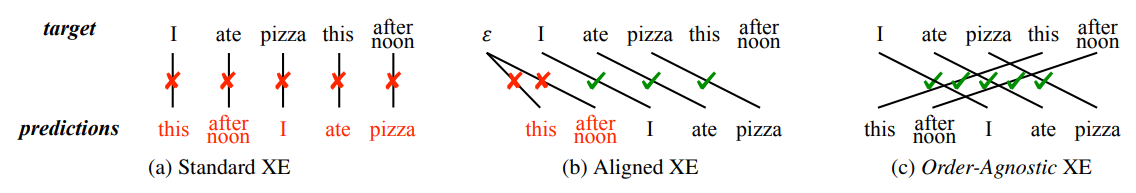
\includegraphics[width=\textwidth]{img/oaxe.png}

  \caption{An illustration of (a) cross-entropy, (b) aligned cross-entropy, and
    (c) order-agnostic cross-entropy on a toy example. We use the figure from
    \citet{du2021orderagnostic}, Figure 1}%
  \label{fig:oaxe-example}
\end{figure}

The dynamic programming algorithm used in the \ac{ctc} and \ac{axe} methods is
no longer suitable for non-monotonic alignments. Moreover, the search space is
even larger than in the previous case as it is proportional to the factorial of
the target length. The authors use the Hungarian algorithm
\citep{kuhn1955hungarian}, which finds a maximum bipartite matching
representing the alignment in polynomial time. They also incorporate heuristics
and tweak the search algorithm to exclude invalid orderings or predictions.

% ----------------------------------------------------------------------------
\paragraph{Imputer.} Antoher variant of the alignment-based approach was
described by \citet{saharia-etal-2020-non}. They experiment with a
\acs{ctc}-based model similar to the model we use in Chapter
\ref{chap:nar-nmt-ctc}, and an iterative variant called \emph{Imputer}.

The model architecture is a stack of self-attentive layers without the causal
mask. The \acs{ctc}-based model takes upsampled source sentence embeddings (in
order to be able to create translations which are longer than the source) and
processes them with the Transformer layer stack.  The Imputer model proceeds in
a fixed number $L$ of iterations. In each iteration, the model generates
(``imputes'') $\ceil*{\frac{T_y}{L}}$ on some positions where $T_y$ is the
output length. This procedure is similar to decoding from \aclp{mlm} described
in Section \ref{sec:nat:semi}. Additionally to the \ac{ctc} model, the input to
the Imputer model is the embedding of the partially decoded sentence from the
previous iteration summed with the (upsampled) source sentence embeddings.

The training of the Imputer model takes into account every partial output
potentially already decoded and maximizes a log-likelihood lower bound, which
can be comptued with a dynamic programming algorithm. \JH{less? put something
  to 3.4?}

% ------------------------------------------------------------------------------
\section{Auxiliary Training Objective Methods}%
\label{sec:nat:aux}
% ------------------------------------------------------------------------------

Auxiliary training objectives can be viewed as a form of regularization of the
training process. Unlike techniques that aim at improving convergence speed,
such as $L_2$ regularization or dropout, the objectives described here are
designed to help \acl{nar} models cope with the conditional independence
assumption in order to better model the target language.

The following methods are based on including one or more auxiliary objectives
into the training procedure. Unlike methods in Sections
\ref{sec:nat:alignment}, \ref{sec:nat:semi} and \ref{sec:nat:misc} which also
use auxiliary objectives, none of these methods changes the decoding process:
Decoding simply takes the highest-scoring token for each time step in parallel.

% ------------------------------------------------------------------------------
\paragraph{\Ac{nat} with Auxiliary Regularization.}
\citet{wang-etal-2019-nonautoregressive} analyze the basic \ac{nat} model
\citep{gu2017nonautoregressive} and identify two frequent translation errors --
repeated and incomplete translation. For each of these symptoms, they design a
special auxiliary training objective to mitigate their effect.

For the repeated translation problem, where the same token is generated
multiple times in conseutive time steps, the authors propose to increase the
dissimilarity of adjacent hidden states when different tokens should be
decoded, tiyng the similarity of the target token embeddings to the similarity
of the corresponding hidden states.

The incomplete translation problem is a case of target tokens missing from the
predicted translation. To address this problem, reverse \ac{ar} translation
model is used to reconstruct the source sentence back from the \ac{nar} decoder
states. The loss of this backward translation model is again used as an
auxiliary objective.

In the final \acs{natreg} model of \citet{wang-etal-2019-nonautoregressive},
the two auxiliary losses are mixed in with the standard cross-entropy loss,
using weight hyperparameters which are set empirically.

% ------------------------------------------------------------------------------
\paragraph{\Acs{hintnat}.} As mentioned in the introductory section of this
chapter, knowledge distillation is often used in \ac{nat}
research. \citet{li-etal-2019-hint} decide to use an \ac{ar} teacher model to
provide signals (hints) to the training of the \ac{nar} student model.

They propose to use two types of hints from the teacher model. First, to bring
the values of the teacher and student decoder hidden states closer together,
the authors consider tying the states with $L_1$ or $L_2$ distance, but argue
that this straightforward approach destabilizes the student training process
and fails. Instead, they use a weaker signal from the teacher model and define
an auxiliary loss based on the cosine distances within the decoder hidden
states. Second, they use the information from the teacher model cross-attention
to guide the alignment learning in the student model. Again, this information
is incorporated into the training as an auxiliary loss, based on the KL
divergence between the teacher and student attention distributions.  Again, the
auxiliary losses are mixed using weighting hyperparameters together with the
cross-entropy loss. \JH{explain the losses}

% -----------------------------------------------------------------------------
\paragraph{\Acl{bon} Difference.} \citet{shao2020minimizing} address the issue
of misalignment between the targets and the outputs. They define the \ac{bon}
difference between the model output distributions and the target sentence, and
instead of finding an appropriate alignment, they design a new objective to
minimize the \ac{bon} difference.

The \ac{bon} objective is based on the $L_1$ distance between two sparse
vectors representing the n-grams which are present in the reference sentence
and are likely to be present in the translation (based on the output
probabilities). As in the previous two cases, this objective is complemented by
the cross-entropy objective. The authors also show that fine-tuning with the
\ac{bon} objective alone is helpful.

% -----------------------------------------------------------------------------
\paragraph{Glancing Training.} \citet{qian-etal-2021-glancing,
  qian2021volctrans} propose \acf{glat}\glsunset{glat}, a technique for
training the \ac{nat} model similarly to \acp{cmlm}, but enabling decoding in a
single pass instead of an iterative process.

During training, the model first generates an intermediate output sentence
non-autoregressively, without computing the loss. Then, a number of positions
is masked according to a glancing sampling strategy, and the model is trained
to predict the masked tokens on the selected positions. The sampling strategy
randomly selects $S$ positions, where $S$ is proportional to the number of
errors in the intermediate prediction.

The decoding is similar to the parallel process proposed by
\citet{gu2017nonautoregressive} described in Section \ref{sec:nat:principles},
but instead of a fertility model, the target sequence length prediction is done
using the output representation of an artificial \texttt{LENGTH} token which is
added to the decoder input (as in the \ac{cmlm} approach of
\citealp{ghazvininejad-etal-2019-mask}, see Section \ref{sec:nat:semi}).

% Very recently, a \ac{glat} model appeared among the top-scoring models at the
% \acs{wmt} news translation shared task \citep{qian2021volctrans}. \JH{update
%   bib after WMT}


% ------------------------------------------------------------------------------
\section{Iterative and Semi-Autoregressive Methods}%
\label{sec:nat:semi}
% ------------------------------------------------------------------------------

The common theme in all of the approaches described so far is that during
inference, the underlying Transformer model is executed only once.  \Acl{ar}
models, on the other hand, need $T_y$ consecutive executions (passes through
the network) to generate a sentence of $T_y$ tokens. This linear relationship
follows from the conditional dependency (see Equation
\ref{eq:output-distribution} in Section \ref{sec:encdec:transformer}).

In this section, we look at methods that lie somewhere in between. In these
approaches, the number of model executions is greater than one, but it is still
constant with respect to the target length $T_y$. We call these approaches
\emph{iterative}. We also include approaches which operate in a fraction of
$T_y$ steps, even though the number of steps is no longer constant. We refer to
these approaches as \emph{semi-autoregressive}.

Many of the methods described here are based on the ideas of iterative
refinement first introduced by \citet{lee-etal-2018-deterministic}, which we
have already reviewed in Section \ref{sec:nat:principles}.

% ------------------------------------------------------------------------------
\paragraph{Iterative Decoding from Masked Language Models.} Recently,
pre-trained \acp{mlm} such as BERT \citep{devlin-etal-2019-bert} have attracted
attention from the translation research
community. \citet{ghazvininejad-etal-2019-mask} introduce
\acfp{cmlm}\glsunset{cmlm}, an extension to \aclp{xlm}
(\acsp{xlm}\glsunset{xlm}; \citealp{conneau-lample-2019-cross}) for
multilingual applications, including \ac{mt}.

Conventional \acp{lm} estimate the probability of a word given the preceding
words.  In contrast, \acp{mlm} are trained on sentences where a number of
tokens have been masked-out, and the objective is to predict what the masked
words were, given the rest of the sentence. \Acp{xlm} extend this idea to a
pair of sentences in two (or more) languages. That is, tokens from either the
source, or the target sentence, or both, are masked and the model tries to
predict them.  To facilitate alignment modeling and language identification,
\ac{xlm} architectures include a language embedding and reset the positional
encodings for each sentence. See Figure \ref{fig:mlm-xlm-example} for an
illustration of the monolingual and cross-lingual \ac{lm} training objectives.

\begin{figure}
  \centering

  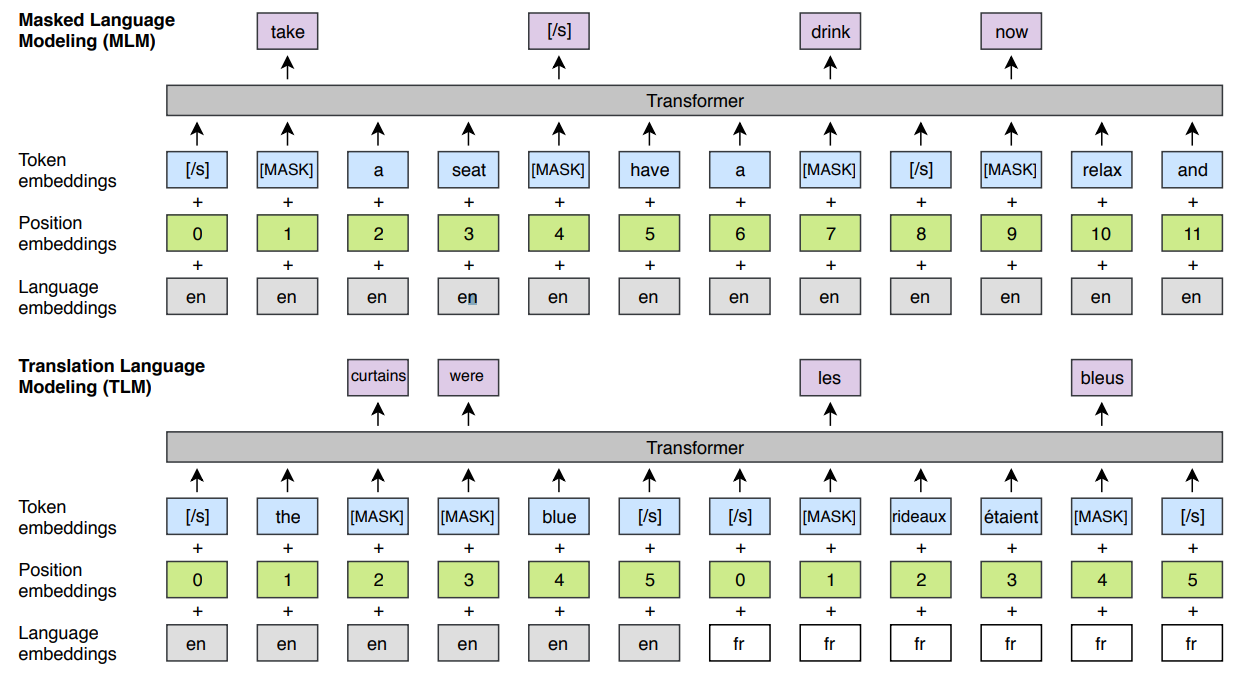
\includegraphics[width=\textwidth]{img/mlm-xlm.png}

  \caption{A comparison of masked language model and translation language model
    training objectives for training \aclp{xlm}. Image source:
    \citet{conneau-lample-2019-cross}, Figure 1.}%
  \label{fig:mlm-xlm-example}
\end{figure}

Compared to the original formulations of \acp{xlm}, \acp{cmlm} differ in a few
aspects: First, \acp{cmlm} use an encoder-decoder architecture, rather than a
decoder-only model that works on the concatenation of the source and target
sentences. Second, only the target words are masked and subject to the training
and prediction. \Acp{cmlm} are also intended to use directly for language
generation, rather than for cross-lingual \ac{lm} pretraining, as is the case
of \acp{xlm}.

The decoding process (called \emph{Mask-Predict}) starts with the estimation of
the target length. For this purpose, \citet{ghazvininejad-etal-2019-mask}
include a special \texttt{LENGTH} token in the decoder input and predict the
target length as the output on this position. This way the length predictor can
be trained jointly with the translation model using the cross entropy training
signal. The authors show that it is useful to sample a small number of
different length candidates, decode a translation for each length, and then
pick the highest scoring one.

Given a target length, the generation begins with a sequence of mask symbols.
In each iteration, the tokens on all masked positions are predicted in parallel
(independently, and thus, non-autoregressively). Then, a number of the tokens
that receive the lowest probability by the model are selected and masked-out
again, prepared to be re-predicted in the next iteration. The number of the
masked tokens is decreasing with each iteration, so that a constant number of
iterations is needed to generate the whole translation.

In their generalized framework for sequence generation,
\citet{mansimov2019generalized} experiment with other masking strategies for
\acp{cmlm}, such as left-to-right, easy-first, or uniform.

% ------------------------------------------------------------------------------
\paragraph{\Acl{smart}.} In their follow-up experiments,
\citet{ghazvininejad-etal-2020-semiautoregressive} address the exposure bias
issue in the context of \acp{cmlm}
% (although they use the terms autoregressive and non-autoregressive for the
% distinction between using the model predictions during training and teacher
% forcing).
As discussed in Section \ref{sec:training}, the exposure bias problem arises
when the model is trained on ground-truth data, but during decoding, it relies
on its own (often incorrect) decisions instead. \Acp{cmlm} are trained to
predict masked tokens given the ground-truth context, but during decoding, the
refinement is done using generated context instead.

To tackle this issue, \citet{ghazvininejad-etal-2020-semiautoregressive}
propose to mix the ground-truth tokens with the model predictions. This
approach is somewhat similar to scheduled sampling for \aclp{rnn}
\citep{bengio2015scheduled}.

% ------------------------------------------------------------------------------
\paragraph{\Acl{disco}.} \citet{kasai2020nonautoregressive} extend the
\ac{cmlm} model with a few additions. Instead of predicting only the masked
tokens, the authors propose an architecture that is able to predict a subset of
the \emph{other} tokens for each position in the target sequence. They achieve
this goal by adapting the attention module. First the self-attention does not
attend to its own position in the sequence on the previous layer. Second, to
prevent information leakage between the same positions on different layers, the
self-attention keys and values are decontextualized, meaning that instead of
hidden states from the previous layer, the decoder input embeddings are
used. \JH{explain more clearly}

% ------------------------------------------------------------------------------
\paragraph{\Acl{jmnat}.} Following the practice from training
the BERT model \citep{devlin-etal-2019-bert}, \citet{guo-etal-2020-jointly}
mask source tokens in the encoder in each step to achieve a more robust encoder
representation. They introduce an auxiliary loss in the encoder for predicting
the masked tokens.

Instead of masking out random tokens in the decoder, the authors propose to
mask whole random n-grams. They also use an additional auxiliary n-gram loss
tailored to help with the problem of repeated tokens in the translation (see
Section \ref{sec:nat:aux}). The Mask-Predict strategy
(\citealp{ghazvininejad-etal-2019-mask}, see above) is employed during
inference.

% ------------------------------------------------------------------------------
\paragraph{Semi-Autoregressive \acs{nmt}.} One of the first attempts to bring
together the best of the worlds of \ac{ar} and \ac{nar} models was proposed by
\citet{wang-etal-2018-semi}. They use a semi-autoregressive Transformer model
which predicts groups of $K$ consecutive tokens at a time. The tokens in each
group are predicted independently and in parallel, but the conditional
dependency is retained between the groups in an autoregressive fashion.

As expected, the authors find that increasing $K$ leads to degraded translation
quality, but brings improvements in terms of decoding speed.

% ------------------------------------------------------------------------------
\paragraph{Blockwise Parallel Decoding for Deep Autoregressive Models.}
\citet{stern2018blockwise} propose a similar semi-autoregressive approach where
chunks of the target sentence are generated in parallel.
%
They start with greedy decoding from an autoregressive model, $p_1$, and
introduce additional ``look-ahead'' models $p_2, \ldots p_k$. In time step $t$,
each model $p_i$ predicts the $(t + i)$-th word in the target sequence given
the same prefix of $t$ previously decoded words.

The decoding process has three stages. First, the block of predictions using
the models $p_1, \ldots, p_k$ is computed. Second, model $p_1$ is used to
verify the $(k-1)$ candidates (which is done in parallel in the Transformer
model) and finds the largest $\hat{k}$ such that decoded words from models
$p_i$, $1 \leq i \leq \hat{k}$ are all considered best by $p_1$. Third, the
accepted $\hat{k}$ words are generated and the decoding process moves to time
step $t + \hat{k}$. \JH{explain more clearly?}

% ------------------------------------------------------------------------------
\paragraph{Insertion Transformer.} The Insertion Transformer
\citep{stern-etal-2019-insertion} is an extension of the Transformer model
which handles sequence generation in an arbitrary order. Instead of predicting
tokens left-to-right, the model predicts sequences of insertion operations. An
insertion operation specifies which tokens to insert and where to insert
them. In each step, the insertion operations are generated in parallel and
independently, we can thus include this approach in the semi-autoregressive
category. The authors experiment with decoding in a balanced binary-tree order,
which can generate the output sequence in a logarithmic number of steps.

% An extension to the Insertion Transformer is
% KERMIT. \citep{chan-etal-2019-kermit} \JH{more about kermit}

% ------------------------------------------------------------------------------
\paragraph{\acl{levt}.} An interesting combination of the ideas introduced in
the Insertion Transformer and \acp{cmlm} is the \acl{levt}
(\acs{levt}\glsunset{levt}; \citealp{gu-etal-2019-levenshtein}). This model
operates in an iterative fashion, much like the aforementioned methods. At the
beginning, \ac{levt} takes either an empty sentence or a crude, intermediate
sentence for refinement. Each iteration consists of applying three
policies. First, tokens to be deleted are identified and removed from the
sequence. Second, the sentence is expanded by placeholder symbols. For each
slot (a position between two tokens), the model decides how many placeholders
to insert. Third, for each placeholder, a token from the vocabulary is selected
to replace it, resulting in a refined version of the input sentence.  Each of
the three stages of a refinement iteration is performed non-autoregressively.

% ------------------------------------------------------------------------------
\paragraph{Latent Transformer.} \citet{kaiser2018fast} use discrete latent
variables in a model called \acf{lt}\glsunset{lt}. The model has three
components: First, the \emph{autoencoder} takes a sentence pair $(x, y)$ and
encodes the target sentence $y$ into a sequence of discrete latent variables
$l$. Second, the \acl{ar} \emph{latent prediction} model predicts the sequence
$l$ based on the source sentence $x$. Third, a \acl{nar} \emph{decoder}
generates $y$ given the source sentence $x$ and the hidden sequence $l$.

The autoencoder is used to condense the longer target sequence $y$ into a
(usually 8 times) shorter sequence $l$, which serves as an itermediate
representation of $y$. Unlike perhaps more common autoencoders, this
autoencoder uses discrete latent variables.
% The authors propose two methods (decomposed vector quantization and latent
% semantic hashing) for the discretization.
A stack of convolutions with residual connections is selected as the
autoencoder architecture. The latent prediction model is a stack of Transformer
layers, and the decoder consists of deconvolutions. \JH{explain how inference
  works, begin with why is this iterative}


% ------------------------------------------------------------------------------
\section{Other Methods}%
\label{sec:nat:misc}
% ------------------------------------------------------------------------------

In this section, we summarize the related work that does not fall clearly
within any of the three categories from the sections above.

% \paragraph{LaNMT} \citep{shu2020latent} -- latent-variable NAR NMT with
% deterministic inference using a delta posterior \JH{to bych nechal na potom
% nebo vyhodil}

% -----------------------------------------------------------------------------
\paragraph{\Acl{dcrf}.} %\textbf{CRF decoding on top of vanilla NAT, not really NAT
% (similar to CTC+beam)}
In the original \ac{nat} model, the generation of the output sentence is done
by selecting the tokens with the highest probability in each position. Instead
of the argmax decoding, \citet{sun2019fast} propose to use \ac{crf}, which
allows the modeling of causal relations within the output sequence. Although
this process is not \acl{nar} given the nature of the \ac{crf} decoding, the
Transformer model needs to be run only once and does not need to take into
account the tokens as they are being generated.

In Section \ref{sec:ctc:fluency} we present a similar idea based on a
\ac{ctc}-based model, using rescoring with an n-gram \acl{lm}.

% -----------------------------------------------------------------------------
\paragraph{Flowseq.} % \textbf{latent variables}
\citet{ma-etal-2019-flowseq} propose to incorporate an intermediate latent
variable $z$ into the model. The authors argue that the prior distribution
$p(z|x)$ needs to be complex to model all dependency relations among the target
tokens. They propose to use generative flow \citep{rezende2015variational} for
deriving the complex distribution from a simple prior using a series of
invertible transformations. \JH{throw out completely?}
% \JH{megacomplex paper}

% -----------------------------------------------------------------------------
\paragraph{Iterative knowledge distillation.}
The common way of adressing the multimodality problem is knowledge distillation
using an \acl{ar} teacher (see Section \ref{sec:training:methodology}).
\citet{sun2020em} propose to iterate the knowledge distillation step. They
alternate the training of the \ac{ar} teacher model and the \ac{nar} student
model in an EM fashion, where the selection of samples for the \ac{ar} training
dataset is informed by the log-likelihood as modeled by the \ac{nar} model. In
this way, the level of multimodality in the distilled corpus is lower and thus
\ac{nar} models trained on this corpus should perform better.

The decoding from the \ac{nar} student model is performed in a single step.
Additionally, the authors propose \acf{odd} which tackles the issue of repeated
outputs while preserving the predicted output length and finds the optimal
sequence without repetition.

% -----------------------------------------------------------------------------
\paragraph{ReorderNAT.} \citet{ran-etal-2021-guiding} introduce an intermediate
Transformer block to model a reoredered source sentence for translation to the
target language.

Formally, the translation model $p(y|x)$ is altered by including a latent
variable $z$ (a sequence of source token embeddings on new positions) which is
marginalized out:
%
\begin{equation}
  p(y|x) = \sum_{z} p(z|x) p(y|z,x)
\end{equation}
%
where $p(z|x)$ is the reordering module, and $p(y|z,x)$ is a \ac{nar}
Transformer decoder which receives the sequence $z$ on the input. The authors
experiment with both \ac{ar} and \ac{nar} variants of the reordering module,
concluding that using a single-layer autoregressive Transformer decoder
performs best while still retaining speed improvements.

The reordering module is trained in supervised fashion using the
\texttt{fast\_align} alignment tool \citep{dyer-etal-2013-simple}. The model is
trained end to end by minimizing the sum of the reordering and decoder module
losses.

% -----------------------------------------------------------------------------
\paragraph{Layer-Wise Prediction with Deep Supervision.}  %\textbf{fully NAT}
A recent approach by \citet{huang-etal-2021-nonautoregressive} uses grounding
of the Transformer hidden states in all layers to the target sentence. On every
decoder layer, the model estimates the output probability distributions from
the hidden states using a linear projection and a softmax layer. From these
layer-level output distributions, the embeddings of the most probable tokens
are added to the input to the next layer along with the hidden state values.

The deep supervision grounds the states of all layers, not just the last one,
to the ground-truth target sequence. The objective function is extended to
include the cross entropies of the layer-wise softmax predictions on all
Transformer layers in the decoder stack.


% ------------------------------------------------------------------------------
\section{Discussion}%
\label{sec:nat:discussion}
% ------------------------------------------------------------------------------

In the conclusion to this chapter, we take a high-level view on the approaches
we have presented here. We point out a few aspects that most of the literature
has in common, as well as some issues regarding the evaluation and comparison
to meaningful baselines.

\JH{add some more to the intro -- summary, problems, following chapters}

% -----------------------------------------------------------------------------
\paragraph{Results.} Table \ref{tab:related:wmt14} shows selected results of
the described approaches on English $\rightarrow$ German \ac{mt}, measured on
the \acs{wmt}~14 test set, which is regarded as the standard benchmark. From
each paper, we select the best result in terms of \acs{bleu}, and a result of a
purely \acl{nar} variant (i.e., without rescoring or additional iterations), if
applicable.

We can see that rescoring using an \acl{ar} teacher consistently helps the
translation performance. However, the more rescoring steps are taken, the less
decoding speed is gained. \JH{There should be a table with the decoding speeds,
  and there should be a figure showing the pareto-frontier. The thing is, no
  such graph would make much sense given the arguments presented below.}

\begin{table}
  \centering

  \begin{adjustbox}{totalheight=\textheight-3\baselineskip}
  \begin{tabular}{cl>{\ignorecolumn}r@{}cc}
    \toprule
    \multicolumn{2}{l}{Method}
    & Steps & En $\rightarrow$ De & De $\rightarrow$ En \\
    \midrule

    & \citet{gu2017nonautoregressive} & & & \\
    & \quad \acs{nat} + FT & 1 & 17.69 & 21.47 \\
    & \quad \acs{nat} + FT + top-100 \acs{npd} rescoring & 101 & 19.17 & 23.20 \\

    & \citet{lee-etal-2018-deterministic} & & \\
    & \quad 1 iteration & 1 & 13.91 & 16.77 \\
    & \quad 10 iterations & 10 & 21.61 & 25.48 \\

    \midrule
    \multirow{6}{*}{\rotatebox{90}{Alignment}}

    & \citet{ghazvininejad2020aligned}, \acs{axe} \acs{cmlm} & 1 & 23.53 & 27.90 \\

    & \citet{du2021orderagnostic}, \acs{cmlm} + \acs{oaxe}
           & \JH{1?} & 26.10 & 30.20 \\

    & \citet{saharia-etal-2020-non} & & & \\
    & \quad \acs{ctc} & 1 & 25.70 & 28.10 \\
    %& \quad Imputer  &  1 & 25.80 & 28.40 \\
    & \quad Imputer & 8 & 28.20 & 31.80 \\

    & \citet{gu-kong-2021-fully}, \acs{nat} + \acs{ctc} + \acs{glat}
           & 1\JH{?} & 27.20 & 31.39 \\

    \midrule
    \multirow{10}{*}{\rotatebox{90}{Auxiliary Objectives}}

    & \citet{wang-etal-2019-nonautoregressive} & & & \\
    & \quad \acs{natreg}, no rescoring & 1 &  20.65 & 24.77 \\
    & \quad \acs{natreg}, top-9 rescoring & 10 & 20.65 & 24.77 \\

    & \citet{li-etal-2019-hint} & & & \\
    & \quad \acs{hintnat}, no rescoring & 1 & 21.11  & 25.24 \\
    & \quad \acs{hintnat}, top-9 rescoring & 10 & 25.20  & 29.52 \\

    & \citet{shao2020minimizing}, \acs{bon}-Joint+FT & \JH{1} & 20.90 & 24.61 \\

    & \citet{qian-etal-2021-glancing} & & & \\
    & \quad \acs{glat} + \acs{ctc} & 1 & 26.39 & 29.54 \\
    & \quad \acs{glat} + \acs{ctc} + top-7 \acs{npd} rescoring & \JH{discuss} & 26.55 & 31.02 \\

    \midrule
    \multirow{10}{*}{\rotatebox{90}{Iterative}}

    & \citet{ghazvininejad-etal-2019-mask} & & \\
    & \quad \acs{cmlm} + Mask-Predict, 1 iteration & 1 & 18.05 & 21.83 \\
    & \quad \acs{cmlm} + Mask-Predict, 10 iterations & 10 & 27.03 & 30.53 \\

    & \citet{kasai2020nonautoregressive}, \acs{disco} + Easy-First
           & \JH{??} & 27.34 & 31.31 \\

    & \citet{guo-etal-2020-jointly} & & & \\
    & \quad \acs{jmnat}, 4 iterations & 4 & 27.05 & 31.51 \\
    & \quad \acs{jmnat}, 10 iterations & 10 & 27.69 & 32.24 \\

    & \citet{kaiser2018fast} & & \\
    & \quad \acs{lt}, no rescoring & 1 & 19.80 & -- \\
    & \quad \acs{lt}, top-100 rescoring & 101 & 22.50 & -- \\

    \midrule
    \multirow{11}{*}{\rotatebox{90}{Other}}

    & \citet{sun2019fast} & & & \\
    & \quad \acs{nat} + \acs{dcrf}, no rescoring & 1 & 23.44 & 27.22 \\
    & \quad \acs{nat} + \acs{dcrf}, top-19 rescoring & 20 & 26.80 & 30.04 \\

    & \citet{ma-etal-2019-flowseq} & & & \\
    & \quad FlowSeq-large & 1 & 23.72 & 28.39 \\
    & \quad FlowSeq-large + top-30 \acs{npd} rescoring & 31 & 25.31 & 30.68 \\

    & \citet{sun2020em}, \acs{emodd} & \JH{??} & 24.54 & 27.93 \\

    & \citet{ran-etal-2021-guiding} & & &  \\
    & \quad \acs{ar} reordering & N & 26.49 & 31.13  \\
    & \quad \acs{nar} reordering & 1\footnotemark\JH{..} & 22.79 & 27.28 \\

    & \citet{huang-etal-2021-nonautoregressive}, CTC + DSLP &\JH{?} & 27.02  &  31.61 \\
    \bottomrule
  \end{tabular}
  \end{adjustbox}
  \caption{The results (in terms of \acs{bleu}) of the described models
    measured on the \acs{wmt}~14 test set, as reported by the authors.}%
  \label{tab:related:wmt14}
\end{table}

% -----------------------------------------------------------------------------
\paragraph{Capturing Reordering.} Many papers referenced in this section claim
that non-autoregressive models cannot capture reordering, which is seen as the
main culprit of the low translation quality of the vanilla \acs{nat} model
\citep{gu-kong-2021-fully, ran-etal-2021-guiding}.  While this might be true to
an extent, we see the multimodality problem as the root cause.  We argue that
reordering itself can be modeled by stacks of self-attentive layers, and if the
space of possible target sentences is less multimodal, reordering is not a big
problem for a \acs{nat} model, as illustrated by \citet{du2021orderagnostic}.

However, the effect of reordering on data complexity is intuitive.
\citet{zhou-etal-2020-understanding} view the amount of reordering in a
translation dataset as a predictor of its complexity and show that knowledge
distillation reduces the reordering score, leading to a simpler dataset, and
thus reducing the multimodality.

% -----------------------------------------------------------------------------
\paragraph{Translation Quality.} Weak \acl{ar} baseline models are a common
element in the \acl{nar} literature. In most cases, the base variant of the
Transformer model is used as baseline (and most of the base hyperparameters are
used for the \ac{nat} model as well), arguing that having similar numbers of
parameters makes the baseline and the \ac{nat} model comparable. A comparable
model size is a valid point; on the other hand, it raises doubts about the
scalability of the proposed approaches -- the difference between large \ac{ar}
and \ac{nar} model variants might not be proportional.

Moreover, even the Transformer base model can be trained in a better way than
as reported by \citet{vaswani2017attention} and as referenced by many \ac{nat}
papers as their baseline, achieving a better translation quality
\citep{popel-bojar-2018-training}.

% -----------------------------------------------------------------------------
\paragraph{Decoding Speed.} Similarly to the previous paragraph, baselines that
appear in the literature are usually weak also in terms of decoding speed.  For
example, \citet{gu2017nonautoregressive} report a latency of 408 ms for their
\ac{ar} model (a Transformer base), measured on a single Nvidia P100 GPU,
without batching. In contrast, our implementation achieves latency of around
100 ms with the same model under the same hardware and hyperparameter settings
and no optimizations. Additionally, most papers cite a baseline \ac{ar} latency
of 607 ms \JH{konkretne kdo}, which is the result of
\citet{gu2017nonautoregressive} with beam search, even though beam search is
not used in the presented \ac{nar} models for the most part.

% \JH{this is regarding the baseline decoding speeds
%   reported by NAT literature. This paragraph should look into WNGT 20 or 21 and
%   check the speeds of best AR results and compare to the autoregressive speeds
%   reported in the NAT literature. What do we find is, that the AR baselines in
%   NAT models are actually much slower. Often, which is another issue, the
%   decoding speeds are not reported at all.  }

% \JH{dalsi vec je ze setup GPU batch 1 hodne zvyhodnuje neautoregresivni modely}


% -----------------------------------------------------------------------------
\paragraph{Evaluation Methodology.} Another aspect we need to address is the
evaluation methodology itself. Setting aside the fact that automatic quality
evaluation using \acs{bleu} is the only reported metric, perhaps complemented
by a cursory manual evaluation on a small sample, the evaluation of the speed
improvements is inconsistent and sometimes the interpretation of the results is
outright wrong.

The main problem is that the actual decoding speed depends on lots of factors
that are not easily reproducible. The most obvious factor is perhaps the
hardware on which the decoding speed is measured, followed by the
implementation. The average decoding time per sentence is also heavily
influenced by the batch size in batched decoding. Table
\ref{tab:related:hardware} shows that these conditions vary wildly within the
literature.

\begin{table}
  \centering

  \begin{tabular}{llcr}
    \toprule
    Publication & GPU type & CPU? & Batch \\
    \midrule
    \citet{gu2017nonautoregressive} & P100 & \xmark & 1 \\
    \citet{lee-etal-2018-deterministic} & P100 or P40 & \cmark & 1  \\
    \citet{kaiser2018fast} & GTX 1080 & \xmark  & 1, 64  \\
    \citet{ghazvininejad-etal-2019-mask} & Possibly V100 & \xmark  & 10 \\
    \citet{sun2019fast} & P100 & \xmark & 1    \\
    \citet{wang-etal-2019-nonautoregressive} & P100 & \xmark & 1    \\
    \citet{li-etal-2019-hint} & Possibly M40 & \xmark  & 1   \\
    \citet{ma-etal-2019-flowseq} &  TITAN X & \xmark &  {\it various}    \\
    \citet{ghazvininejad2020aligned} & {\it Not reported} & \xmark  & {\it unknown}  \\
    \citet{shao2020minimizing} &  TITAN X & \xmark  & 1   \\
    \citet{guo-etal-2020-jointly} & GTX 1080 Ti & \xmark & 1    \\
    \citet{kasai2020nonautoregressive} & V100 & \xmark & 1    \\
    \citet{qian-etal-2021-glancing} & GTX 1080 Ti & \xmark  & 1?  \\
    \citet{ran-etal-2021-guiding} & P40 & \xmark & 1   \\
    \citet{gu-kong-2021-fully} & V100 & \cmark  & 1   \\
    \citet{du2021orderagnostic} & {\it Not reported} & \xmark  & 1   \\
    \citet{huang-etal-2021-nonautoregressive} & V100 & \xmark & 1   \\
    \bottomrule
  \end{tabular}

  \caption{The hardware setting and decoding batch size for measuring the
    decoding speed as reported in a sample of papers described in this
    section.}%
  \label{tab:related:hardware}
\end{table}

A popular solution that takes the varying conditions into account for
evaluating decoding speed is to report the relative speed-up measured between
experiments within a single study. However, comparing these relative speed-up
ratios between different papers disregards the actual decoding times -- it is
easier to achieve 20 times speed-up over a slow baseline than over a baseline
which is faster.

It is, however, challenging to find a way to compare the contributions of
different reserch groups objectively. One such effort is made by the organizers
of the Efficiency Shared Task, now organized yearly at the \acl{wmt}
(\acs{wmt}\glsunset{wmt}, \citealp{heafield-etal-2020-findings,
  heafield-etal-2021-findings}).\JH{update bib when ready, separate WMT from cite}

In the Efficiency Shared Task, submissions are evaluated both in terms of
translation quality and the decoding speed under various settings. All
submissions are evaluated on the same hardware, hosted by Amazon Web Services.
To amortize the effects of data and model loading, the decoding time is
measured on a dataset which contains one million sentences. The speed is
measured in five different scenarios: GPU latency (decoding without batching)
and throughput (decoding with the optimal batch size), latency and throughput
on a single CPU, and throughput on a multi-core CPU. \JH{shrnout poznatky ze shared tasku}

% \JH{This paragraph will discuss the
%   evalutaion in general. Reporting relative speed-up OK, but citing
%   autoregressive latency by others and then measure speed up relative to that
%   is not OK, as well as citing and comparing to relative speed-ups of others.
%   Most papers report GPU latency, but it is not a rule. The speed should be
%   reported under multiple settings, best would be to report it as they do in
%   WNGT, i.e. latency and throughput (batching and no-batching), and both on CPU
%   and on GPU. Also, they should always say how many cores they used.}

% \JH{We could also have a table with autoregressive baselines reported by each
%   study, and get some details on that.}

Our final observation is that measuring latency on a single GPU without
batching is a setup that favorizes \ac{nar} models, even though other scenarios
should also be considered for real-world applications. In batched GPU decoding,
the differences between \ac{ar} and \ac{nar} models fade, because
batch-parallelization of \ac{ar} models makes up for time-parallelization of
\ac{nar} models. On the other hand, in an online decoding scenario on a CPU,
only limited parallelization is possible, so the advantage of \ac{nar} models
is also diminished. \JH{observation je na zaklade vysledku, odkaz na kapitolu}



%\JH{perhaps add something about time complexity and how it is not constant?}

% \begin{table}
%   \centering

%   \begin{tabular}{lll}
%     \toprule
%     Method & Steps & \acs{bleu} \\
%     \midrule

%     \bottomrule
%   \end{tabular}

%   \caption{An overview of the \ac{nat} models in the literature.}%
%   \label{tab:related-models}
% \end{table}

%%% Local Variables:
%%% mode: latex
%%% TeX-master: "thesis"
%%% End:

% %%%%%%%%%%%%%%%%%%%%%%%%%%%%%%%%%%%%%%%%%%%%%%%%%%%%%%%%%%%%%%%%%%%%%%%%%%%%%
\chapter{Non-Autoregressive NMT with Connectionist Temporal Classification}
\label{chap:nar-nmt-ctc}
% %%%%%%%%%%%%%%%%%%%%%%%%%%%%%%%%%%%%%%%%%%%%%%%%%%%%%%%%%%%%%%%%%%%%%%%%%%%%%

\paperdisclaim{This chapter is based on paper ``End-to-End Non-Autoregressive
  Neural Machine Translation with Connectionist Temporal Classification'',
  joint work with Jindřich Libovický, published at EMNLP 2018.}

\noindent
In this chapter, we lay grounds for the \ac{nar} approaches studied in this
thesis. We describe our experiments with an architecture based on the \ac{ctc}
loss \citep{libovicky-helcl-2018-end}. \JH{ok to self-cite when sections will
  be based on this?} \JH{use \ac{nat} here somewhere}


We begin with the description of the \ac{ctc} algorithm for compute the
cross-entropy loss over all possible alignments between the reference sentence
and the sequence of output states in Section \ref{sec:ctc}. Section
\ref{sec:ctc:arch} introduces the proposed \ac{nat} model architecture based on
the Transformer model \citep{vaswani2017attention}. The results of the
preliminary experiments and the limitations are discussed in Section
\ref{sec:ctc:experiments}. In Section \ref{sec:ctc:fluency}, we present our
attempt to address the most severe issue non-autoregressive models have, which
is the reduced fluency compared to the autoregressive models
\citep{kasner2020improving,kasner2020incorporating}.

% -----------------------------------------------------------------------------
\section{Connectionist Temporal Classification}
\label{sec:ctc}
% -----------------------------------------------------------------------------

\Ac{ctc} \citep{graves2006connectionist} is a method for training neural
networks on sequential data. Originally applied to the phonetic labelling task,
but later successfully adapted in related areas, including \ac{asr} or
handwriting recognition \citep{liwicki2007novel, eyben2009speech,
  graves2014towards}.

The main strength of \ac{ctc} becomes evident in tasks where the input and
output labels are weakly or not at all aligned, for example in situations where
the observed input sequence is considerably longer than the target output
sequence -- hence the application to \ac{asr}, where the number of extracted
features per second is higher than the number of phonemes uttered per second.
\JH{Confirm this.}

Training neural networks with \ac{ctc} is independent on the actual neural
network architecture. The \ac{ctc} loss function can be applied on any network
with sequential outputs. Thus, this method is applicable to both \acp{rnn} and
the Transformer model.

Models trained with the \ac{ctc} assume that the alignment between the input
(e.g. a group of frames in an audio signal) and the output (e.g. a phoneme)
states is unknown. A variable number of frames in a row can encode a single
phoneme. Similarly, in translation, multiple words in the source language may
correspond to any number of (even non-consecutive) words in the target
language.

The idea behind \ac{ctc} is to allow some states to produce no output. This is
realized by introducing a special blank token in the target vocabulary.
Optionally, identical outputs produced by multiple consecutive states may be
merged and considered a single output. Because of these properties, there are
groups of equivalent output sequences, which all represent the same target, as
illustrated in Figure~\ref{fig:ctc-equivalent-sequences}.

\begin{figure}
  \centering
  \begin{minipage}{\textwidth}
    \begin{equation*}
        \text{a cat sat on a mat} =
        \begin{cases}
          & \text{a <blank> cat sat on a <blank> mat} \\
          & \text{a a cat cat sat on a mat} \\
          & \text{a <blank> cat cat sat on a mat} \\
        \end{cases}
    \end{equation*}
  \end{minipage}
  \caption{A group of output sequences of equal length which all represent the
    same target in CTC.} %
  \label{fig:ctc-equivalent-sequences}
\end{figure}

In the standard sequence-to-sequence architectures, the value of the loss
function is defined as the sum of the cross entropies of each output state with
respect to the target sequence (see Equation \ref{eq:loss}). In \ac{ctc}, the
loss is defined as the sum of cross-entropy losses of all of the output
sequences equivalent to the given target sequence:
%
\begin{equation}
  J_{\theta}^{\text{CTC}} = - \sum_{(x, y) \in D} \sum_{y' \sim y}  \log p(y' | x, \theta)
  \label{eq:ctc-loss}
\end{equation}
%
where $\sim$ denotes the equivalence relation.  \JH{$J_{\theta}$ should perhaps
  be $J(\theta)$. Also, consider the $\sim$ sign.}

The inner summation in Equation \ref{eq:ctc-loss} is computed over all possible
sequences equivalent to the label sequence. For technical purposes, the label
sequences are limited to a fixed length, which greatly reduces the number of
acceptable hypotheses. However, the number of equivalent hypotheses of a given
length still grows exponentially with the sequence length -- in \ac{ctc}, the
fixed length is always set to be longer than the label sequence. \JH{confirm
  the exponential claim}

The summation over the large set of equivalent sequences can be
implemented using dynamic programming. When both the length of the output and
the length of the target sequences are known, there is a constant number of the
blank tokens to be generated. The process of computing the loss of the whole
output sequence is divided into computing the partial losses with respect to
the possible label prefixes.

\begin{figure}
  \centering

  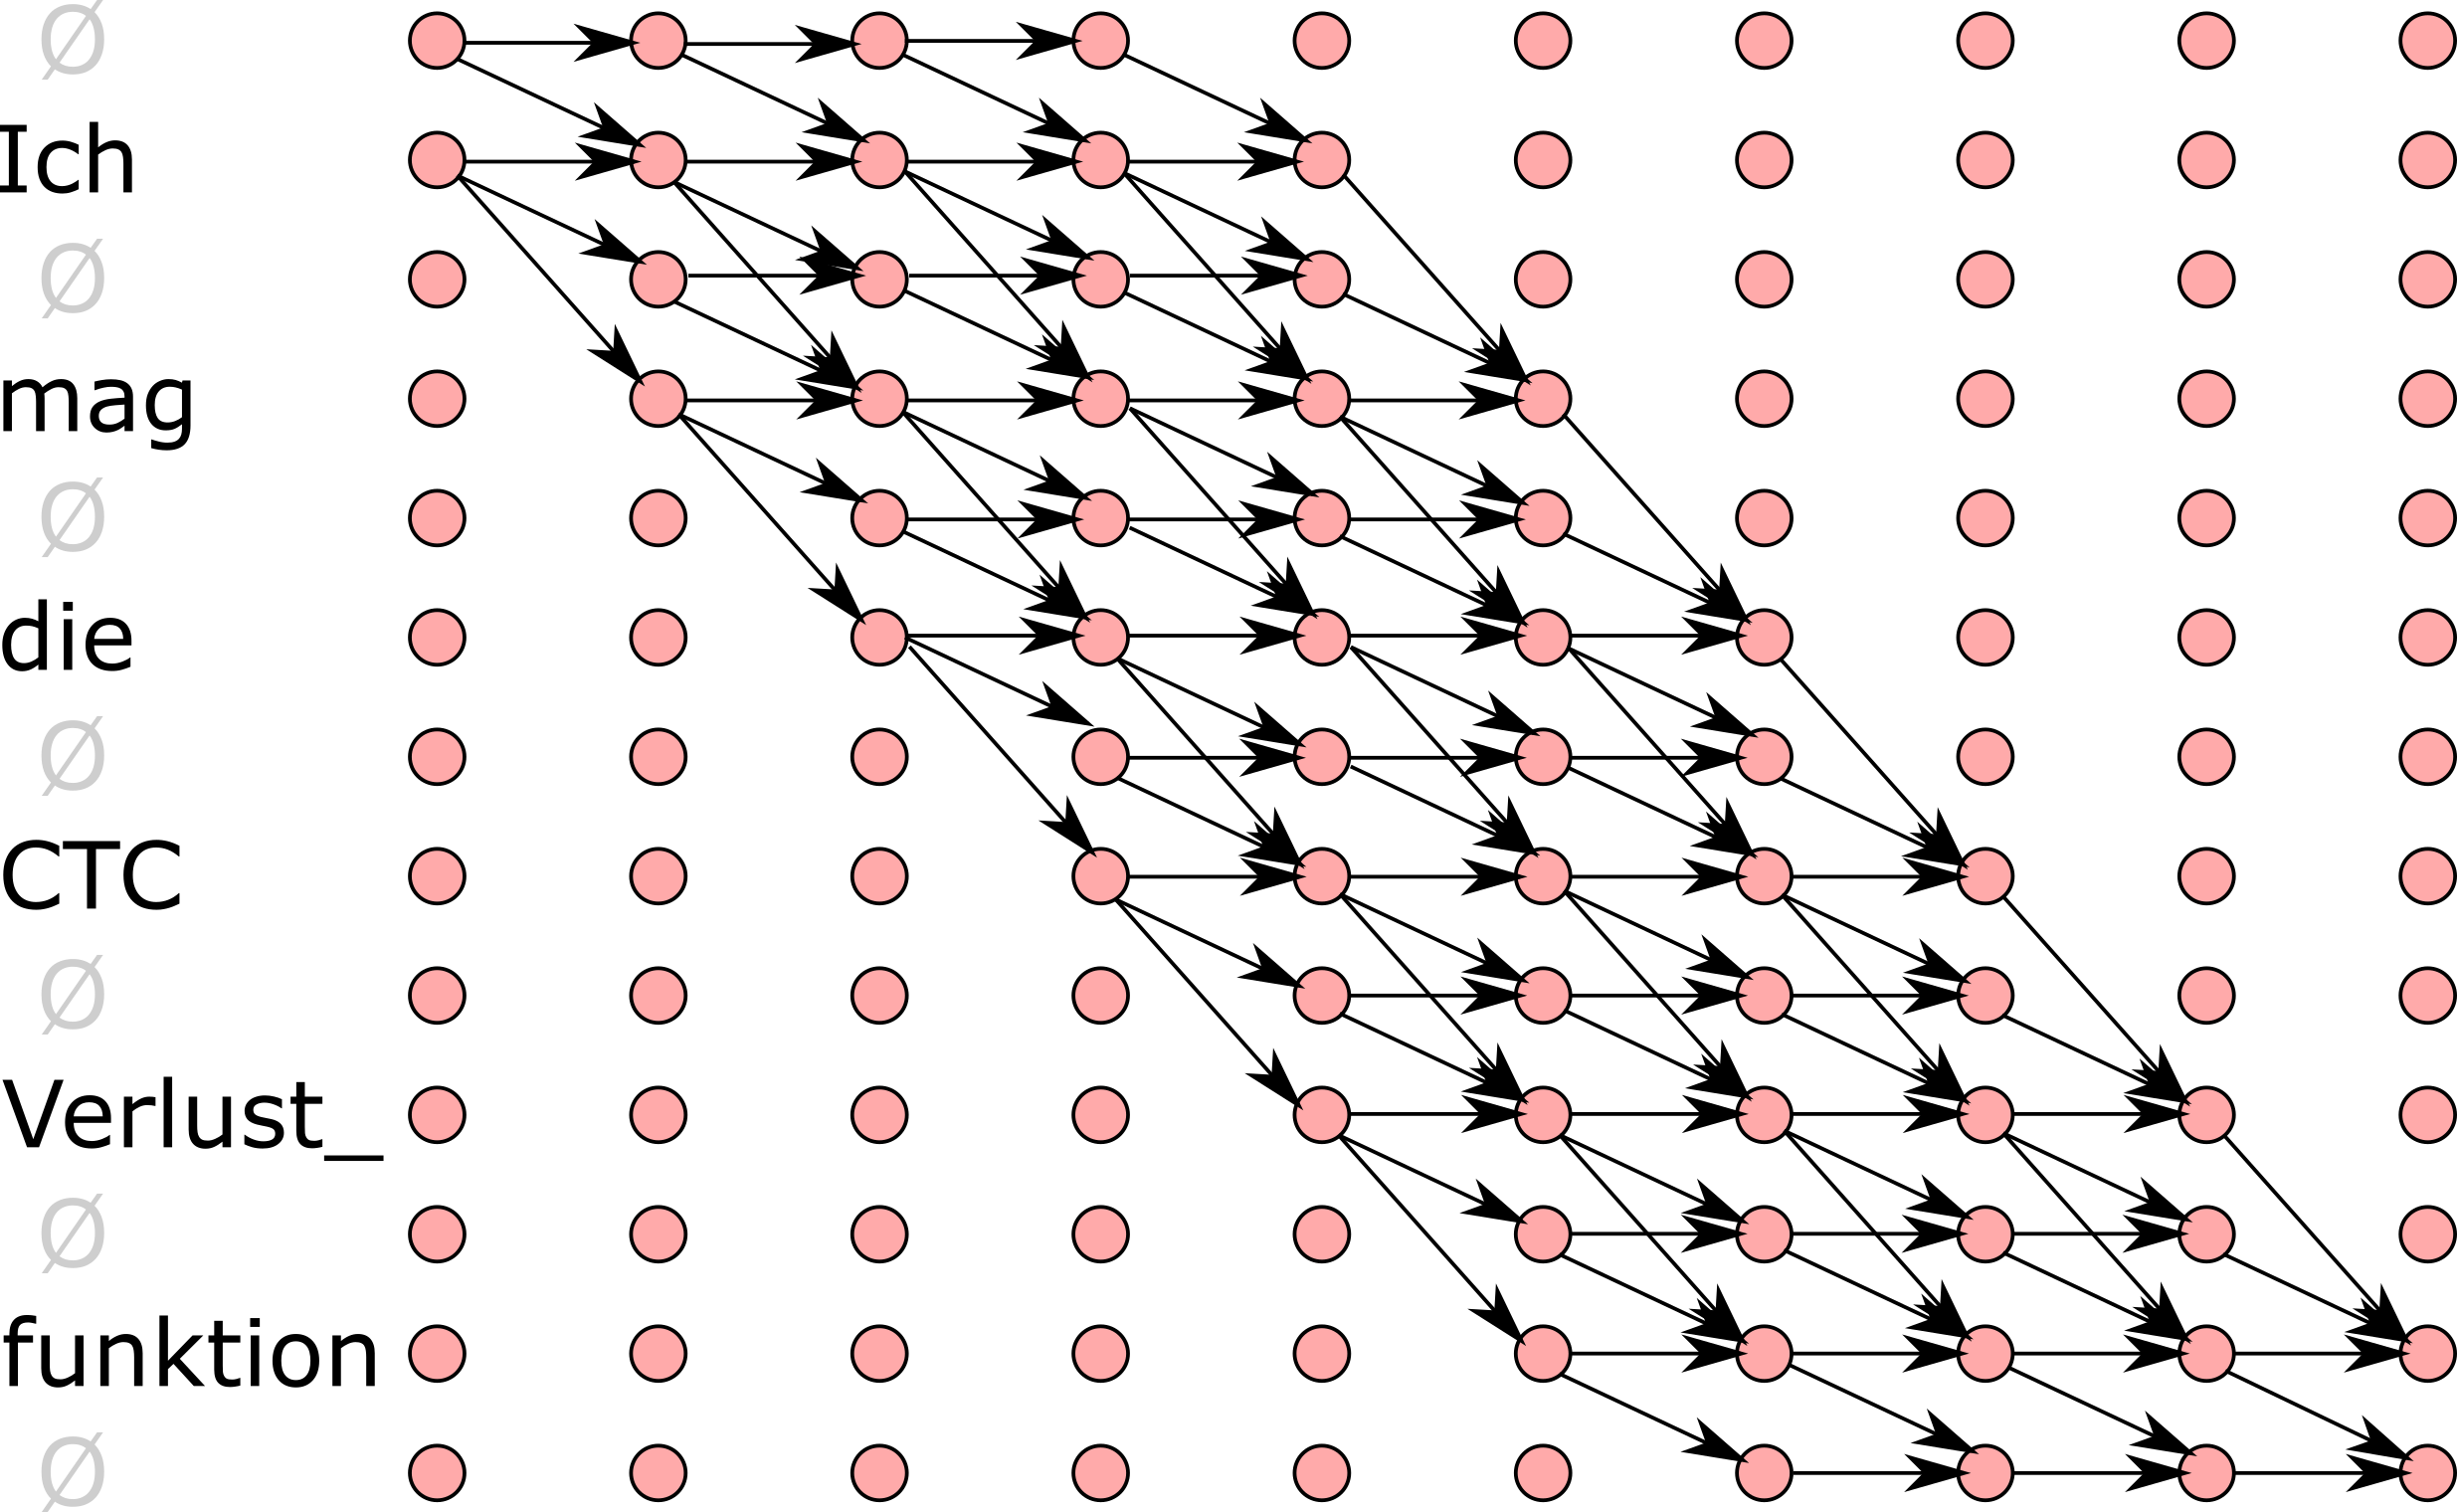
\includegraphics[width=13cm]{img/ctc_schema.png}

  \caption{An illustration of the algorihm for the CTC loss computation. Each
    node denotes producing either a token from the label sequence, or the blank
    token. Each path from one of the two top-left nodes to one of the two
    bottom-right nodes corresponds to one of the equivalent sequences.  }
  \label{fig:ctc-dynamic-programming}
\end{figure}

The \ac{ctc} loss computation is illustrated in Figure
\ref{fig:ctc-dynamic-programming}. The rows represent tokens from the label
sequence plus the optional blank tokens. The columns represent the output state
sequence.  Each node in the graph denotes generating a label from an output
state. The arrows show valid transitions between the generation steps. An arrow
can only go down one or two rows, or horizontally.  The horizontal arrows
denote repeated generation of the same label. These labels are later merged to
form a single output. An arrow can only go two rows down when the skipped row
corresponds to the blank token, so no target tokens are left out. Each path in
the diagram therefore shows one of the equivalent sequences that lead to
generating the given label sequence.

Using the idea that many of the paths from left to right in the diagram share
segments, we can apply dynamic programming to compute the sum of losses across
all paths without the need to enumerate each of them. A node on coordinates
$(i,j)$ stores the accumulated losses for the all path prefixes that lead to
the node, added with the negative log likelihood of the label on the $i$-th row
being generated by the $j$-th output state. The two bottom-right nodes then
store the sum of losses of all the paths.


\JH{doplnit} The training of the network with \ac{ctc} is done by minimizing
the \ac{ctc} loss function, which is defined as follows.

% -----------------------------------------------------------------------------
\section{Model Architecture}
\label{sec:ctc:arch}
% -----------------------------------------------------------------------------

As said in the previous chapter, training models with \ac{ctc} does not impose
any requirements on the model architecture. In our experiments, we aim for a
reasonable comparison between our proposed approach and the state-of-the-art
autoregressive models. We adapt the Transformer model and use similar
hyperparameters where applicable.

Non-autoregressive models generate the outputs in parallel, which requires that
the output length is known beforehand. In autoregressive models, the end of
sequence is indicated by a special end symbol, and the constraint on maximum
length is merely a technical aspect.

To leverage the ability to output empty tokens to the full extent, the output
length should be set to a higher number than the length of the target sequence.
Since the length estimation does not need to be accurate, we select a number
$k$ and we set the target sequence length to be $k$ times longer than the
source length. Note that in case the selected length is shorter than the label
sequence, the model will not be able to generate the whole target sequence.

\begin{figure}
  \centering
  \def\inputsize{7}

\begin{tikzpicture}[]

\draw (\inputsize / 2 + 0.1, -0.1) node {Input token embeddings};

\foreach \i in {0,...,\inputsize} {
	\draw (\i,-0.5) rectangle (\i+0.2,-1);
    \draw [->] (\i+0.1,-1) -- (\i+0.1, -1.25);
};

\draw (0, -1.25) rectangle (\inputsize + 0.2, -2.25);
\draw (\inputsize / 2 + 0.1, -1.75) node {Encoder};

\foreach \i in {0,...,\inputsize} {
	\draw [->] (\i+0.1,-2.25) -- (\i+0.1, -2.5);
    \draw[fill=yellow!40] (\i,-2.5) rectangle (\i+0.2,-3);

    \draw [->] (\i+0.1,-3) -- (\i+0.1, -3.25);
	\draw[fill=blue!40] (\i,-3.25) rectangle (\i+0.2,-3.75);
	\draw[fill=red!40] (\i,-3.75) rectangle (\i+0.2,-4.25);

    \draw [dashed,->] (\i+0.1,-4.25) -  - (\i+0.1, -4.75);
    \draw [dashed,->] (\i+0.2,-3.5) .. controls (\i + 0.6, -3.65) .. (\i+0.6, -4.75);

	\draw[fill=red!40] (\i,-4.75) rectangle (\i+0.2,-5.25);
	\draw[fill=blue!40] (\i + 0.5,-4.75) rectangle (\i+0.7,-5.25);

    \draw [->] (\i+0.1,-5.25) - - (\i+0.1, -5.5);
    \draw [->] (\i+0.6,-5.25) - - (\i+0.6, -5.5);
};

\draw (\inputsize + 1.2, -2.75) node {$\mathbf{h}$};
\draw (\inputsize + 1.2, -3.75) node {$W_{\text{spl}}\mathbf{h}$};
\draw (\inputsize + 1.2, -5.00) node {$\mathbf{s}$};

\draw (0, -5.5) rectangle (\inputsize + 0.7, -6.5);
\draw (\inputsize / 2 + 0.5 + 0.1, -6.0) node {Decoder};

\draw [fill=green!80!black!60] (\inputsize / 2 + 0.4,-7.2) circle [x radius=\inputsize / 2 + 0.4, y radius=0.5];
\draw (\inputsize / 2 + 0.6, -7.2) node {Connectionist Temporal Classification};

\foreach \i in {0,...,\inputsize} {
   \draw [->] (\i+0.1,-7.9) - - (\i+0.1, -8.15);
   \draw [->] (\i+0.6,-7.9) - - (\i+0.6, -8.15);
}

\draw  (0+0.1,-8.4) node {$w_1$};
\draw  (0+0.6,-8.4) node {$w_2$};
\draw  (1+0.1,-8.4) node {$w_3$};
\draw  (1+0.6,-8.4) node {$\varnothing$};
\draw  (2+0.1,-8.4) node {$w_4$};
\draw  (2+0.6,-8.4) node {$\varnothing$};
\draw  (3+0.1,-8.4) node {$w_5$};
\draw  (3+0.6,-8.4) node {$w_6$};
\draw  (4+0.1,-8.4) node {$\varnothing$};
\draw  (4+0.6,-8.4) node {$\varnothing$};
\draw  (5+0.1,-8.4) node {$\varnothing$};
\draw  (5+0.6,-8.4) node {$w_7$};
\draw  (6+0.1,-8.4) node {$w_8$};
\draw  (6+0.6,-8.4) node {$\varnothing$};
\draw  (7+0.1,-8.4) node {$w_9$};
\draw  (7+0.6,-8.4) node {$\varnothing$};

\draw (\inputsize / 2 + 0.3, -8.95) node {Output tokens / null symbols};

\end{tikzpicture}

  \caption{The scheme of the non-autoregressive architecture with
    state-splitting and CTC. The image is taken from
    \citet{libovicky-helcl-2018-end}.}%
  \label{fig:state-splitting}
\end{figure}


We implement the source-to-target length expansion by linear projections and
state splitting. This mechanism is illustrated in Figure
\ref{fig:state-splitting}. After a given Transformer layer completes its
computation, we linearly project the states
$h_1, \ldots, h_{T_x} \in \mathbb{R}^d$ into $\mathbb{R}^{kd}$. Then, we split
each of these projections into $k$ parts, which results to a $k$-times longer
sequence of states $s_1, \ldots, s_{k \cdot T_x}$ of the original dimension
$d$:
%
\begin{equation}
  s_{ck+b} = \left( W_{\text{spl}} h_c + b_{\text{spl}} \right)_{bd:(b+1)d}
\end{equation}
%
for $b=0 \ldots k-1$ and $c=1 \ldots T_x$ where
$W_{\text{spl}} \in \mathbb{R}^{d \times kd}$ and
$b_{\text{spl}} \in \mathbb{R}^{kd}$ are the trainable projection parameters.

We experiment with two placement options of the state splitting layer. First,
we try placing the state splitting at the end of the Transformer layer
stack. In this scenario, there are 12 Transformer encoder layers, followed by
the state splitting layer, whose outputs are used in the output
projection. Second, we place the state splitting layer in the middle of the
Transformer layer stack, mimicking the 6-layer encoder-decoder architecture of
the autoregressive Transformer model. In the second variant, cross-attention
can be included in the second half of the layers, which attends to the states
right after state splitting.

% -----------------------------------------------------------------------------
\section{Preliminary Experiments}%
\label{sec:ctc:experiments}
% -----------------------------------------------------------------------------

\JH{Section with experiments from the 2018 paper. Should show that it works,
  but it's still far from perfect.}

We conduct experiments with \ac{ctc}-based \ac{nat} models trained on
English--German and English--Romanian translation in both directions.

\paragraph{Data.}
In our experiments, we use the parallel data provided by the \acs{wmt}
organizers. For English--German, the training data consist of the Europarl
corpus \citep{koehn-2005-europarl}, News commentary
\citep{tiedemann-2012-parallel}, and Common
Crawl.\footnote{\url{https://commoncrawl.org/}} For validation, we use the
WMT~13 test set \citep{bojar-etal-2013-findings}, and we evaluate the
translation quality on the WMT~14 test set
\citep{bojar-etal-2014-findings}. For English--Romanian, the data consist of
the Europarl corpus, and the SETIMES corpus distributed by OPUS
\citep{tiedemann-2012-parallel}. We use the development and test set from
WMT~16 \citep{bojar-etal-2016-findings}. The data sizes are shown in
Table~\ref{tab:end-to-end:data}.

\begin{table}
  \centering
  \begin{tabular}{lrr}
    \toprule
     & Sentence pairs & Vocabulary size \\
    \midrule
    En -- De & 4.58 M & 41,488 \\
    En -- Ro & 613 k & 38,440 \\
    \bottomrule
  \end{tabular}

  \caption{The training data sizes. \JH{more}}%
  \label{tab:end-to-end:data}
\end{table}

We preprocess the data with scripts from the \texttt{mosesdecoder}
repository,\footnote{\url{https://github.com/moses-smt/mosesdecoder/}} a part
of the Moses translation toolkit \citep{koehn-etal-2007-moses}. Namely, we
normalize the punctuation in the data, then we use the tokenizer and a
truecaser. We segment the data using the wordpiece algorithm, creating a
vocabulary of approximately 41k wordpieces for English--German, and 38k
wordpieces fro English--Romanian \citep{wu2016google}.

\paragraph{Models and Training.}
We implement and train our models in the Neural Monkey toolkit
\citep{helcl-libovicky-2017-neural,helcl-etal-2018-neural}. Neural Monkey is a
higher-level deep learning toolkit implemented in TensorFlow
\citep{tensorflow2015-whitepaper}, aiming for fast prototyping using
simple-format configuration files. We train all models for 10 epochs and we
select the best-scoring model based on the validation BLEU score. The training
of the En--De models on a single Nvidia GeForce GTX 1080 GPU took approximately
4 weeks. Since the En--Ro parallel data was much smaller, the training of the
En--Ro models took 4 days.

We summarize the model and training settings in Table
\ref{tab:end-to-end:hparams}. Note that the architecture resembles the
Transformer big settigns, but uses a smaller model dimension. We use the same
settings for training models in both directions in both language pairs.

\begin{table}
  \centering
  \begin{tabular}{lr}
    \toprule
    Parameter & Value \\
    \midrule
    No. of encoder layers & 6 \\
    No. of decoder layers & 6 \\
    Model dimension & 512 \\
    Attention heads & 16 \\
    Dropout probability & 0.1 \\
    Feed-forward hidden size & 4,096 \\
    State splitting factor & 3 \\
    State splitting projection size & 1,536 \\
    Vocabulary size & See Table \ref{tab:end-to-end:data} \\
    \midrule
    Optimizer method & adam \\
    $\beta_1$ & 0.9 \\
    $\beta_2$ & 0.997 \\
    $\epsilon$ & 10\textsuperscript{-9} \\
    Learning rate & 10\textsuperscript{-4} \\
    Fixed batch size & 20 \\
    Gradient clipping & 1 \\
    \bottomrule
  \end{tabular}

  \caption{Experimental settings for the Neural Monkey experiments.}%
  \label{tab:end-to-end:hparams}
\end{table}

\paragraph{Results.} Table \ref{tab:end-to-end:bleu} compares the quantitative
results of our non-autoregressive models with methods proposed by
\citet{gu2017nonautoregressive} and \citet{lee-etal-2018-deterministic}. We use
the SacreBLEU \citep{post-2018-call} to compute the BLEU scores of the model
outputs.

\begin{table}
  \centering
  \begin{tabular}{lcccc}
    \toprule
     & \multicolumn{2}{c}{WMT~16} & \multicolumn{2}{c}{WMT~14} \\
     & En $\rightarrow$ Ro & Ro $\rightarrow$ En & En $\rightarrow$ De & De $\rightarrow$ En \\
    \midrule
    \citet{gu2017nonautoregressive} & & & & \\
    Autoregressive baseline & 31.35 & 31.03 & 22.71 & 26.39 \\
    \addlinespace
    NAT + FT & 27.29 & 29.06 & 17.69 & 21.47 \\
    NAT + FT + NPD (100 s) & 29.79 & 31.44 & 19.17 & 23.20 \\
    \midrule
    \citet{lee-etal-2018-deterministic} & & & & \\
    Autoregressive baseline & 31.93 & 31.55  & 23.77 & 28.15 \\
    \addlinespace
    1 iteration & 24.45 & 25.73 & 13.91 & 16.77 \\
    10 iterations & 29.32 & 30.19 & 21.61 & 25.48 \\
    \midrule
    \citet{libovicky-helcl-2018-end} & & & & \\
    Autoregressive baseline & 21.19 & 29.64 & 22.94 & 28.58 \\
    \addlinespace
    Deep encoder & 17.33 & 22.85 & 12.21 & 12.53 \\
    \quad + weight averaging & 18.47 & 24.68 & 14.65 & 16.72 \\
    \quad + beam search & 18.70 & 25.28 & 15.19 & 17.58 \\
    \addlinespace
    Encoder-decoder  & 18.51 & 22.37 & 13.29 & 17.98 \\
    \quad + weight averaging & 19.54 & 24.67 & 16.56 & 18.64 \\
    \quad + beam search & 19.81 & 25.21 & 17.09 & 18.80  \\
    \addlinespace
    Encoder-decoder with pos. enc. & 18.13 & 22.75 & 12.51 & 11.35 \\
    \quad + weight averaging & 19.31 & 24.21 & 17.37 & 18.07 \\
    \quad + beam search & 19.93 & 24.71 & 17.68 & 19.80 \\
    \bottomrule
  \end{tabular}

  \caption{Automatic evaluation of our \acs{ctc}-based approach, compared to
    the two of the first non-autoregressive methods, along with autoregressive
    greedy-decoding baseline scores. }%
  \label{tab:end-to-end:bleu}
\end{table}

The first model of \citet{gu2017nonautoregressive} represents the \ac{nat}
model with fine-tuning, which minimizes the KL divergence between the output
distributions of the teacher and student models. In the second row, \ac{npd}
with 100 samples is used. \JH{This should be described in Related work.} Using
\ac{npd} can slow down the decoding, because an additional scoring step by an
autoregressive model is needed. In theory, if enough parallelism is available,
this doubles the latency.

The approach of \citet{lee-etal-2018-deterministic} is iterative. We show the
performance of this method with 1 iteration and with 10 iterations. Note that
using more iterations slows down the decoding speed of the iterative model.

When compared to the single-pass models, the performance of the English--German
\acs{ctc}-based models is similar. However, the performance of the
English--Romanian models is poor. This is likely because of issues with
Romanian diacritics in the data, as suggested also by the poorer performance of
our autoregressive baseline. Also, the enhanced techniques (\ac{npd} and
iterative refiniment) outperform our method in all scenarios, but at a
computational cost.

\JH{Description of weight averaging and the beam search.}

The decoding speed for \ac{ar} and {nar} models under different conditions is
shown in Table~\ref{tab:end-to-end:speed}. We report the average time to decode
a single sentence on the \ac{wmt}~15 test set \citep{bojar-etal-2015-findings},
which consists of 2,169 sentence pairs. In the CPU setting, we are using a CPU
machine with the TensorFlow session configured to use 12 CPU threads. The GPU
results are measured on a single Nvidia GeForce GTX 1080 GPU. We show the
average latency as well as the average time to decode a sentence when using
batch decoding.
\JH{Compare speed results? Or leave it for the next chapter.}

\begin{table}
  \centering

  \begin{tabular}{lrr}
    \toprule
     & \mc{CPU} & \mc{GPU} \\
    \midrule
    \acs{ar}, batch=1 & 2,247 ms & 1,129 ms \\
    \acs{ar}, batch=100 & & 127 ms\\
    % AR, beam=?
    \addlinespace
    \acs{nar}, batch=1 & 397 ms & 353 ms  \\
    \acs{nar}, batch=100 &  & 41 ms \\
    \bottomrule
  \end{tabular}

  \caption{The average times to decode one sentence under different conditions.}%
  \label{tab:end-to-end:speed}

\end{table}

Figure \ref{fig:end-to-end:speed} shows the decoding latencies on sentences
from the \ac{wmt}~15 test set \citep{bojar-etal-2015-findings}. As we can see
from the relationship between the source sentence length and the decoding time,
the non-autoregressive model exhibits lower time complexity than the
autoregressive model. The latencies in the plot were measured on a CPU server
using 12 threads. We used greedy decoding with a single sentence in a batch.

\begin{figure}
  \centering
  \begin{tikzpicture}[gnuplot]
%% generated with GNUPLOT 5.2p8 (Lua 5.3; terminal rev. Nov 2018, script rev. 108)
%% Tue 12 Oct 2021 04:15:30 PM BST
\path (0.000,0.000) rectangle (9.000,7.000);
\gpcolor{color=gp lt color border}
\gpsetlinetype{gp lt border}
\gpsetdashtype{gp dt solid}
\gpsetlinewidth{1.00}
\draw[gp path] (0.920,0.986)--(1.100,0.986);
\draw[gp path] (8.815,0.986)--(8.635,0.986);
\node[gp node right] at (0.736,0.986) {$0$};
\draw[gp path] (0.920,1.988)--(1.100,1.988);
\draw[gp path] (8.815,1.988)--(8.635,1.988);
\node[gp node right] at (0.736,1.988) {$1$};
\draw[gp path] (0.920,2.990)--(1.100,2.990);
\draw[gp path] (8.815,2.990)--(8.635,2.990);
\node[gp node right] at (0.736,2.990) {$2$};
\draw[gp path] (0.920,3.993)--(1.100,3.993);
\draw[gp path] (8.815,3.993)--(8.635,3.993);
\node[gp node right] at (0.736,3.993) {$3$};
\draw[gp path] (0.920,4.995)--(1.100,4.995);
\draw[gp path] (8.815,4.995)--(8.635,4.995);
\node[gp node right] at (0.736,4.995) {$4$};
\draw[gp path] (0.920,5.997)--(1.100,5.997);
\draw[gp path] (8.815,5.997)--(8.635,5.997);
\node[gp node right] at (0.736,5.997) {$5$};
\draw[gp path] (0.920,6.999)--(1.100,6.999);
\draw[gp path] (8.815,6.999)--(8.635,6.999);
\node[gp node right] at (0.736,6.999) {$6$};
\draw[gp path] (0.920,0.986)--(0.920,1.166);
\draw[gp path] (0.920,6.999)--(0.920,6.819);
\node[gp node center] at (0.920,0.678) {$0$};
\draw[gp path] (2.499,0.986)--(2.499,1.166);
\draw[gp path] (2.499,6.999)--(2.499,6.819);
\node[gp node center] at (2.499,0.678) {$20$};
\draw[gp path] (4.078,0.986)--(4.078,1.166);
\draw[gp path] (4.078,6.999)--(4.078,6.819);
\node[gp node center] at (4.078,0.678) {$40$};
\draw[gp path] (5.657,0.986)--(5.657,1.166);
\draw[gp path] (5.657,6.999)--(5.657,6.819);
\node[gp node center] at (5.657,0.678) {$60$};
\draw[gp path] (7.236,0.986)--(7.236,1.166);
\draw[gp path] (7.236,6.999)--(7.236,6.819);
\node[gp node center] at (7.236,0.678) {$80$};
\draw[gp path] (8.815,0.986)--(8.815,1.166);
\draw[gp path] (8.815,6.999)--(8.815,6.819);
\node[gp node center] at (8.815,0.678) {$100$};
\draw[gp path] (0.920,6.999)--(0.920,0.986)--(8.815,0.986)--(8.815,6.999)--cycle;
\node[gp node center,rotate=-270] at (-0.016,3.992) {decoding time in seconds};
\node[gp node center] at (4.867,0.216) {source subwords};
\gpcolor{rgb color={0.800,0.000,0.000}}
\gpsetlinewidth{5.50}
\draw[gp path] (0.920,1.263)--(1.000,1.336)--(1.079,1.410)--(1.159,1.484)--(1.239,1.558)%
  --(1.319,1.632)--(1.398,1.706)--(1.478,1.780)--(1.558,1.853)--(1.638,1.927)--(1.717,2.001)%
  --(1.797,2.075)--(1.877,2.149)--(1.957,2.223)--(2.036,2.297)--(2.116,2.371)--(2.196,2.444)%
  --(2.276,2.518)--(2.355,2.592)--(2.435,2.666)--(2.515,2.740)--(2.595,2.814)--(2.674,2.888)%
  --(2.754,2.961)--(2.834,3.035)--(2.914,3.109)--(2.993,3.183)--(3.073,3.257)--(3.153,3.331)%
  --(3.233,3.405)--(3.312,3.478)--(3.392,3.552)--(3.472,3.626)--(3.552,3.700)--(3.631,3.774)%
  --(3.711,3.848)--(3.791,3.922)--(3.871,3.996)--(3.950,4.069)--(4.030,4.143)--(4.110,4.217)%
  --(4.190,4.291)--(4.269,4.365)--(4.349,4.439)--(4.429,4.513)--(4.509,4.586)--(4.588,4.660)%
  --(4.668,4.734)--(4.748,4.808)--(4.828,4.882)--(4.907,4.956)--(4.987,5.030)--(5.067,5.103)%
  --(5.147,5.177)--(5.226,5.251)--(5.306,5.325)--(5.386,5.399)--(5.466,5.473)--(5.545,5.547)%
  --(5.625,5.621)--(5.705,5.694)--(5.785,5.768)--(5.864,5.842)--(5.944,5.916)--(6.024,5.990)%
  --(6.104,6.064)--(6.183,6.138)--(6.263,6.211)--(6.343,6.285)--(6.423,6.359)--(6.502,6.433)%
  --(6.582,6.507)--(6.662,6.581)--(6.742,6.655)--(6.821,6.729)--(6.901,6.802)--(6.981,6.876)%
  --(7.061,6.950)--(7.113,6.999);
\gpcolor{rgb color={0.000,0.000,0.800}}
\draw[gp path] (0.920,1.215)--(1.000,1.221)--(1.079,1.227)--(1.159,1.233)--(1.239,1.239)%
  --(1.319,1.244)--(1.398,1.250)--(1.478,1.256)--(1.558,1.262)--(1.638,1.268)--(1.717,1.274)%
  --(1.797,1.280)--(1.877,1.286)--(1.957,1.292)--(2.036,1.298)--(2.116,1.304)--(2.196,1.310)%
  --(2.276,1.316)--(2.355,1.322)--(2.435,1.328)--(2.515,1.333)--(2.595,1.339)--(2.674,1.345)%
  --(2.754,1.351)--(2.834,1.357)--(2.914,1.363)--(2.993,1.369)--(3.073,1.375)--(3.153,1.381)%
  --(3.233,1.387)--(3.312,1.393)--(3.392,1.399)--(3.472,1.405)--(3.552,1.411)--(3.631,1.417)%
  --(3.711,1.422)--(3.791,1.428)--(3.871,1.434)--(3.950,1.440)--(4.030,1.446)--(4.110,1.452)%
  --(4.190,1.458)--(4.269,1.464)--(4.349,1.470)--(4.429,1.476)--(4.509,1.482)--(4.588,1.488)%
  --(4.668,1.494)--(4.748,1.500)--(4.828,1.506)--(4.907,1.511)--(4.987,1.517)--(5.067,1.523)%
  --(5.147,1.529)--(5.226,1.535)--(5.306,1.541)--(5.386,1.547)--(5.466,1.553)--(5.545,1.559)%
  --(5.625,1.565)--(5.705,1.571)--(5.785,1.577)--(5.864,1.583)--(5.944,1.589)--(6.024,1.594)%
  --(6.104,1.600)--(6.183,1.606)--(6.263,1.612)--(6.343,1.618)--(6.423,1.624)--(6.502,1.630)%
  --(6.582,1.636)--(6.662,1.642)--(6.742,1.648)--(6.821,1.654)--(6.901,1.660)--(6.981,1.666)%
  --(7.061,1.672)--(7.140,1.678)--(7.220,1.683)--(7.300,1.689)--(7.380,1.695)--(7.459,1.701)%
  --(7.539,1.707)--(7.619,1.713)--(7.699,1.719)--(7.778,1.725)--(7.858,1.731)--(7.938,1.737)%
  --(8.018,1.743)--(8.097,1.749)--(8.177,1.755)--(8.257,1.761)--(8.337,1.767)--(8.416,1.772)%
  --(8.496,1.778)--(8.576,1.784)--(8.656,1.790)--(8.735,1.796)--(8.815,1.802);
\gpcolor{color=gp lt color border}
\node[gp node right] at (8.083,4.146) {AR};
\gpcolor{rgb color={0.867,0.000,0.000}}
\gpsetlinewidth{0.80}
\gpsetpointsize{4.00}
\gppoint{gp mark 3}{(1.552,2.944)}
\gppoint{gp mark 3}{(5.104,5.179)}
\gppoint{gp mark 3}{(3.131,3.343)}
\gppoint{gp mark 3}{(2.183,2.426)}
\gppoint{gp mark 3}{(2.262,2.860)}
\gppoint{gp mark 3}{(2.736,2.862)}
\gppoint{gp mark 3}{(4.078,4.814)}
\gppoint{gp mark 3}{(4.473,5.662)}
\gppoint{gp mark 3}{(3.446,3.635)}
\gppoint{gp mark 3}{(3.367,3.611)}
\gppoint{gp mark 3}{(3.131,3.330)}
\gppoint{gp mark 3}{(2.262,2.376)}
\gppoint{gp mark 3}{(2.025,2.338)}
\gppoint{gp mark 3}{(2.104,2.468)}
\gppoint{gp mark 3}{(2.104,2.427)}
\gppoint{gp mark 3}{(2.499,2.610)}
\gppoint{gp mark 3}{(3.525,3.064)}
\gppoint{gp mark 3}{(3.289,3.378)}
\gppoint{gp mark 3}{(3.210,3.444)}
\gppoint{gp mark 3}{(2.341,2.666)}
\gppoint{gp mark 3}{(2.183,2.268)}
\gppoint{gp mark 3}{(2.736,3.253)}
\gppoint{gp mark 3}{(4.710,6.120)}
\gppoint{gp mark 3}{(3.525,3.045)}
\gppoint{gp mark 3}{(3.841,4.057)}
\gppoint{gp mark 3}{(4.473,5.371)}
\gppoint{gp mark 3}{(2.104,2.466)}
\gppoint{gp mark 3}{(3.762,3.850)}
\gppoint{gp mark 3}{(4.315,5.573)}
\gppoint{gp mark 3}{(4.078,4.322)}
\gppoint{gp mark 3}{(5.183,5.537)}
\gppoint{gp mark 3}{(4.631,5.557)}
\gppoint{gp mark 3}{(5.025,5.763)}
\gppoint{gp mark 3}{(5.420,6.596)}
\gppoint{gp mark 3}{(3.052,3.635)}
\gppoint{gp mark 3}{(7.157,6.654)}
\gppoint{gp mark 3}{(2.183,2.611)}
\gppoint{gp mark 3}{(5.183,5.542)}
\gppoint{gp mark 3}{(4.552,5.229)}
\gppoint{gp mark 3}{(2.341,2.600)}
\gppoint{gp mark 3}{(1.394,1.760)}
\gppoint{gp mark 3}{(2.499,2.632)}
\gppoint{gp mark 3}{(3.446,3.726)}
\gppoint{gp mark 3}{(2.183,2.684)}
\gppoint{gp mark 3}{(1.552,1.850)}
\gppoint{gp mark 3}{(3.289,3.640)}
\gppoint{gp mark 3}{(2.973,3.125)}
\gppoint{gp mark 3}{(2.025,2.745)}
\gppoint{gp mark 3}{(3.604,4.848)}
\gppoint{gp mark 3}{(4.946,6.315)}
\gppoint{gp mark 3}{(3.210,3.118)}
\gppoint{gp mark 3}{(3.762,4.093)}
\gppoint{gp mark 3}{(2.578,2.908)}
\gppoint{gp mark 3}{(3.446,4.833)}
\gppoint{gp mark 3}{(6.999,6.565)}
\gppoint{gp mark 3}{(3.604,3.556)}
\gppoint{gp mark 3}{(3.525,3.849)}
\gppoint{gp mark 3}{(3.052,3.918)}
\gppoint{gp mark 3}{(4.078,5.196)}
\gppoint{gp mark 3}{(3.920,3.840)}
\gppoint{gp mark 3}{(2.973,3.290)}
\gppoint{gp mark 3}{(3.683,3.995)}
\gppoint{gp mark 3}{(3.367,4.688)}
\gppoint{gp mark 3}{(2.341,3.394)}
\gppoint{gp mark 3}{(3.052,3.897)}
\gppoint{gp mark 3}{(2.578,3.684)}
\gppoint{gp mark 3}{(3.525,4.390)}
\gppoint{gp mark 3}{(4.710,4.821)}
\gppoint{gp mark 3}{(2.104,2.527)}
\gppoint{gp mark 3}{(2.341,2.127)}
\gppoint{gp mark 3}{(4.157,4.015)}
\gppoint{gp mark 3}{(2.499,2.791)}
\gppoint{gp mark 3}{(3.131,3.106)}
\gppoint{gp mark 3}{(3.999,5.824)}
\gppoint{gp mark 3}{(3.683,4.417)}
\gppoint{gp mark 3}{(5.657,6.625)}
\gppoint{gp mark 3}{(3.920,4.043)}
\gppoint{gp mark 3}{(3.052,2.649)}
\gppoint{gp mark 3}{(3.525,3.645)}
\gppoint{gp mark 3}{(1.552,2.005)}
\gppoint{gp mark 3}{(6.999,6.345)}
\gppoint{gp mark 3}{(3.289,3.319)}
\gppoint{gp mark 3}{(5.104,6.225)}
\gppoint{gp mark 3}{(3.762,3.807)}
\gppoint{gp mark 3}{(3.210,3.795)}
\gppoint{gp mark 3}{(4.710,5.241)}
\gppoint{gp mark 3}{(5.025,5.915)}
\gppoint{gp mark 3}{(2.894,3.333)}
\gppoint{gp mark 3}{(3.367,3.564)}
\gppoint{gp mark 3}{(3.131,3.156)}
\gppoint{gp mark 3}{(3.210,3.442)}
\gppoint{gp mark 3}{(2.341,2.593)}
\gppoint{gp mark 3}{(2.894,2.737)}
\gppoint{gp mark 3}{(2.578,2.972)}
\gppoint{gp mark 3}{(1.473,1.879)}
\gppoint{gp mark 3}{(2.341,2.355)}
\gppoint{gp mark 3}{(3.052,2.832)}
\gppoint{gp mark 3}{(3.683,4.284)}
\gppoint{gp mark 3}{(2.499,2.711)}
\gppoint{gp mark 3}{(3.367,3.440)}
\gppoint{gp mark 3}{(3.525,3.704)}
\gppoint{gp mark 3}{(1.394,1.684)}
\gppoint{gp mark 3}{(1.867,2.397)}
\gppoint{gp mark 3}{(3.683,3.708)}
\gppoint{gp mark 3}{(3.446,3.659)}
\gppoint{gp mark 3}{(4.868,5.945)}
\gppoint{gp mark 3}{(3.683,4.462)}
\gppoint{gp mark 3}{(3.131,2.981)}
\gppoint{gp mark 3}{(2.104,2.743)}
\gppoint{gp mark 3}{(2.973,3.581)}
\gppoint{gp mark 3}{(3.841,4.105)}
\gppoint{gp mark 3}{(1.946,2.099)}
\gppoint{gp mark 3}{(1.788,1.928)}
\gppoint{gp mark 3}{(3.367,2.711)}
\gppoint{gp mark 3}{(2.025,1.893)}
\gppoint{gp mark 3}{(1.552,1.713)}
\gppoint{gp mark 3}{(1.946,1.975)}
\gppoint{gp mark 3}{(2.815,2.784)}
\gppoint{gp mark 3}{(3.052,3.539)}
\gppoint{gp mark 3}{(1.552,1.757)}
\gppoint{gp mark 3}{(4.157,4.178)}
\gppoint{gp mark 3}{(4.236,5.400)}
\gppoint{gp mark 3}{(5.025,5.146)}
\gppoint{gp mark 3}{(5.025,5.332)}
\gppoint{gp mark 3}{(3.525,4.143)}
\gppoint{gp mark 3}{(3.289,4.024)}
\gppoint{gp mark 3}{(3.841,3.512)}
\gppoint{gp mark 3}{(2.104,2.071)}
\gppoint{gp mark 3}{(1.394,1.708)}
\gppoint{gp mark 3}{(4.946,5.767)}
\gppoint{gp mark 3}{(4.473,5.009)}
\gppoint{gp mark 3}{(5.341,6.369)}
\gppoint{gp mark 3}{(5.736,6.023)}
\gppoint{gp mark 3}{(2.420,3.003)}
\gppoint{gp mark 3}{(3.210,2.205)}
\gppoint{gp mark 3}{(3.289,3.305)}
\gppoint{gp mark 3}{(3.920,4.366)}
\gppoint{gp mark 3}{(3.210,3.337)}
\gppoint{gp mark 3}{(3.052,3.570)}
\gppoint{gp mark 3}{(4.078,4.673)}
\gppoint{gp mark 3}{(2.736,2.428)}
\gppoint{gp mark 3}{(2.973,3.309)}
\gppoint{gp mark 3}{(3.604,3.451)}
\gppoint{gp mark 3}{(2.736,3.101)}
\gppoint{gp mark 3}{(1.946,2.072)}
\gppoint{gp mark 3}{(4.789,5.801)}
\gppoint{gp mark 3}{(4.315,4.257)}
\gppoint{gp mark 3}{(4.157,4.017)}
\gppoint{gp mark 3}{(2.104,2.221)}
\gppoint{gp mark 3}{(4.157,3.982)}
\gppoint{gp mark 3}{(4.078,3.748)}
\gppoint{gp mark 3}{(1.315,1.661)}
\gppoint{gp mark 3}{(3.604,3.847)}
\gppoint{gp mark 3}{(7.552,6.636)}
\gppoint{gp mark 3}{(1.236,1.564)}
\gppoint{gp mark 3}{(2.262,2.336)}
\gppoint{gp mark 3}{(3.131,2.492)}
\gppoint{gp mark 3}{(5.578,4.543)}
\gppoint{gp mark 3}{(3.762,3.266)}
\gppoint{gp mark 3}{(2.815,2.305)}
\gppoint{gp mark 3}{(4.946,5.147)}
\gppoint{gp mark 3}{(1.078,1.511)}
\gppoint{gp mark 3}{(3.210,3.651)}
\gppoint{gp mark 3}{(3.131,3.103)}
\gppoint{gp mark 3}{(1.631,2.152)}
\gppoint{gp mark 3}{(6.210,6.525)}
\gppoint{gp mark 3}{(3.683,3.502)}
\gppoint{gp mark 3}{(5.104,5.203)}
\gppoint{gp mark 3}{(4.157,4.412)}
\gppoint{gp mark 3}{(2.183,2.170)}
\gppoint{gp mark 3}{(4.157,4.219)}
\gppoint{gp mark 3}{(3.131,2.982)}
\gppoint{gp mark 3}{(3.052,3.685)}
\gppoint{gp mark 3}{(4.631,5.922)}
\gppoint{gp mark 3}{(4.552,5.776)}
\gppoint{gp mark 3}{(2.025,2.377)}
\gppoint{gp mark 3}{(2.025,1.886)}
\gppoint{gp mark 3}{(3.131,3.850)}
\gppoint{gp mark 3}{(3.289,3.827)}
\gppoint{gp mark 3}{(2.262,2.231)}
\gppoint{gp mark 3}{(5.657,6.239)}
\gppoint{gp mark 3}{(2.499,2.837)}
\gppoint{gp mark 3}{(2.183,2.276)}
\gppoint{gp mark 3}{(3.841,3.226)}
\gppoint{gp mark 3}{(3.210,3.582)}
\gppoint{gp mark 3}{(2.420,2.730)}
\gppoint{gp mark 3}{(3.210,4.165)}
\gppoint{gp mark 3}{(2.499,2.606)}
\gppoint{gp mark 3}{(3.841,4.587)}
\gppoint{gp mark 3}{(3.210,4.011)}
\gppoint{gp mark 3}{(5.499,5.924)}
\gppoint{gp mark 3}{(3.210,3.835)}
\gppoint{gp mark 3}{(7.315,4.959)}
\gppoint{gp mark 3}{(4.946,4.239)}
\gppoint{gp mark 3}{(4.946,5.662)}
\gppoint{gp mark 3}{(4.078,4.082)}
\gppoint{gp mark 3}{(2.815,3.296)}
\gppoint{gp mark 3}{(4.631,4.627)}
\gppoint{gp mark 3}{(3.525,3.580)}
\gppoint{gp mark 3}{(2.183,2.463)}
\gppoint{gp mark 3}{(1.631,1.818)}
\gppoint{gp mark 3}{(2.025,2.048)}
\gppoint{gp mark 3}{(2.657,2.088)}
\gppoint{gp mark 3}{(3.052,2.864)}
\gppoint{gp mark 3}{(2.499,2.425)}
\gppoint{gp mark 3}{(6.999,6.966)}
\gppoint{gp mark 3}{(2.499,2.818)}
\gppoint{gp mark 3}{(1.867,1.966)}
\gppoint{gp mark 3}{(4.473,4.515)}
\gppoint{gp mark 3}{(1.788,2.192)}
\gppoint{gp mark 3}{(2.894,3.169)}
\gppoint{gp mark 3}{(3.841,4.028)}
\gppoint{gp mark 3}{(3.289,3.483)}
\gppoint{gp mark 3}{(3.999,4.159)}
\gppoint{gp mark 3}{(2.657,2.903)}
\gppoint{gp mark 3}{(3.999,4.427)}
\gppoint{gp mark 3}{(3.131,3.302)}
\gppoint{gp mark 3}{(3.525,3.764)}
\gppoint{gp mark 3}{(4.236,4.758)}
\gppoint{gp mark 3}{(5.262,4.952)}
\gppoint{gp mark 3}{(5.183,5.952)}
\gppoint{gp mark 3}{(1.867,1.981)}
\gppoint{gp mark 3}{(2.815,2.990)}
\gppoint{gp mark 3}{(2.420,2.904)}
\gppoint{gp mark 3}{(3.762,4.119)}
\gppoint{gp mark 3}{(3.289,3.267)}
\gppoint{gp mark 3}{(2.657,2.335)}
\gppoint{gp mark 3}{(3.210,3.205)}
\gppoint{gp mark 3}{(4.315,4.664)}
\gppoint{gp mark 3}{(3.920,3.858)}
\gppoint{gp mark 3}{(1.236,1.626)}
\gppoint{gp mark 3}{(5.578,5.122)}
\gppoint{gp mark 3}{(6.525,5.554)}
\gppoint{gp mark 3}{(3.052,2.977)}
\gppoint{gp mark 3}{(6.131,6.022)}
\gppoint{gp mark 3}{(5.025,5.077)}
\gppoint{gp mark 3}{(2.736,2.482)}
\gppoint{gp mark 3}{(4.631,4.383)}
\gppoint{gp mark 3}{(2.657,2.851)}
\gppoint{gp mark 3}{(3.052,2.935)}
\gppoint{gp mark 3}{(1.631,1.846)}
\gppoint{gp mark 3}{(1.631,2.233)}
\gppoint{gp mark 3}{(1.710,2.295)}
\gppoint{gp mark 3}{(2.025,2.147)}
\gppoint{gp mark 3}{(4.078,4.263)}
\gppoint{gp mark 3}{(2.973,2.352)}
\gppoint{gp mark 3}{(3.920,4.356)}
\gppoint{gp mark 3}{(2.578,2.801)}
\gppoint{gp mark 3}{(6.052,6.778)}
\gppoint{gp mark 3}{(3.683,3.924)}
\gppoint{gp mark 3}{(3.920,3.508)}
\gppoint{gp mark 3}{(5.262,5.262)}
\gppoint{gp mark 3}{(2.815,2.798)}
\gppoint{gp mark 3}{(3.683,4.368)}
\gppoint{gp mark 3}{(1.946,2.098)}
\gppoint{gp mark 3}{(2.499,2.731)}
\gppoint{gp mark 3}{(2.499,2.523)}
\gppoint{gp mark 3}{(2.341,2.252)}
\gppoint{gp mark 3}{(3.604,3.145)}
\gppoint{gp mark 3}{(2.420,2.521)}
\gppoint{gp mark 3}{(4.631,4.419)}
\gppoint{gp mark 3}{(1.788,2.238)}
\gppoint{gp mark 3}{(3.446,3.371)}
\gppoint{gp mark 3}{(2.499,2.504)}
\gppoint{gp mark 3}{(3.210,3.436)}
\gppoint{gp mark 3}{(2.262,2.226)}
\gppoint{gp mark 3}{(4.394,4.599)}
\gppoint{gp mark 3}{(2.104,2.766)}
\gppoint{gp mark 3}{(1.946,2.086)}
\gppoint{gp mark 3}{(2.499,2.609)}
\gppoint{gp mark 3}{(3.131,2.841)}
\gppoint{gp mark 3}{(2.341,2.386)}
\gppoint{gp mark 3}{(2.657,2.579)}
\gppoint{gp mark 3}{(1.631,1.964)}
\gppoint{gp mark 3}{(3.446,3.307)}
\gppoint{gp mark 3}{(3.762,3.128)}
\gppoint{gp mark 3}{(2.815,3.420)}
\gppoint{gp mark 3}{(3.999,3.188)}
\gppoint{gp mark 3}{(3.131,3.060)}
\gppoint{gp mark 3}{(2.894,2.780)}
\gppoint{gp mark 3}{(2.262,2.481)}
\gppoint{gp mark 3}{(2.657,2.952)}
\gppoint{gp mark 3}{(4.473,4.237)}
\gppoint{gp mark 3}{(2.420,2.333)}
\gppoint{gp mark 3}{(3.683,3.326)}
\gppoint{gp mark 3}{(5.025,4.768)}
\gppoint{gp mark 3}{(4.789,4.646)}
\gppoint{gp mark 3}{(2.499,2.709)}
\gppoint{gp mark 3}{(3.604,3.797)}
\gppoint{gp mark 3}{(2.025,2.166)}
\gppoint{gp mark 3}{(3.525,3.882)}
\gppoint{gp mark 3}{(3.367,3.355)}
\gppoint{gp mark 3}{(5.341,6.181)}
\gppoint{gp mark 3}{(1.867,2.201)}
\gppoint{gp mark 3}{(5.420,5.768)}
\gppoint{gp mark 3}{(4.868,4.606)}
\gppoint{gp mark 3}{(4.631,4.492)}
\gppoint{gp mark 3}{(2.736,2.879)}
\gppoint{gp mark 3}{(6.447,6.654)}
\gppoint{gp mark 3}{(6.289,6.428)}
\gppoint{gp mark 3}{(5.104,5.737)}
\gppoint{gp mark 3}{(6.762,4.954)}
\gppoint{gp mark 3}{(2.341,1.977)}
\gppoint{gp mark 3}{(1.946,2.089)}
\gppoint{gp mark 3}{(1.788,2.008)}
\gppoint{gp mark 3}{(2.736,3.223)}
\gppoint{gp mark 3}{(2.499,2.504)}
\gppoint{gp mark 3}{(4.315,4.318)}
\gppoint{gp mark 3}{(2.578,2.675)}
\gppoint{gp mark 3}{(1.946,2.108)}
\gppoint{gp mark 3}{(3.131,2.728)}
\gppoint{gp mark 3}{(1.473,1.723)}
\gppoint{gp mark 3}{(2.578,2.936)}
\gppoint{gp mark 3}{(1.315,1.688)}
\gppoint{gp mark 3}{(1.078,1.569)}
\gppoint{gp mark 3}{(1.631,1.790)}
\gppoint{gp mark 3}{(5.183,5.202)}
\gppoint{gp mark 3}{(1.710,1.912)}
\gppoint{gp mark 3}{(2.657,2.640)}
\gppoint{gp mark 3}{(4.236,4.328)}
\gppoint{gp mark 3}{(4.552,3.600)}
\gppoint{gp mark 3}{(3.920,3.600)}
\gppoint{gp mark 3}{(3.683,3.990)}
\gppoint{gp mark 3}{(2.262,3.120)}
\gppoint{gp mark 3}{(2.736,2.849)}
\gppoint{gp mark 3}{(3.999,3.972)}
\gppoint{gp mark 3}{(3.052,3.200)}
\gppoint{gp mark 3}{(2.104,2.318)}
\gppoint{gp mark 3}{(1.473,1.875)}
\gppoint{gp mark 3}{(1.710,1.771)}
\gppoint{gp mark 3}{(1.315,1.621)}
\gppoint{gp mark 3}{(2.025,1.764)}
\gppoint{gp mark 3}{(1.710,1.724)}
\gppoint{gp mark 3}{(2.657,2.508)}
\gppoint{gp mark 3}{(1.788,1.736)}
\gppoint{gp mark 3}{(2.104,1.834)}
\gppoint{gp mark 3}{(1.788,1.735)}
\gppoint{gp mark 3}{(1.867,2.098)}
\gppoint{gp mark 3}{(1.710,1.873)}
\gppoint{gp mark 3}{(3.683,3.847)}
\gppoint{gp mark 3}{(2.894,3.139)}
\gppoint{gp mark 3}{(1.631,1.621)}
\gppoint{gp mark 3}{(1.710,1.788)}
\gppoint{gp mark 3}{(1.473,1.919)}
\gppoint{gp mark 3}{(3.367,3.142)}
\gppoint{gp mark 3}{(2.736,2.632)}
\gppoint{gp mark 3}{(2.183,2.215)}
\gppoint{gp mark 3}{(3.052,3.064)}
\gppoint{gp mark 3}{(2.025,2.246)}
\gppoint{gp mark 3}{(2.420,2.690)}
\gppoint{gp mark 3}{(4.315,4.222)}
\gppoint{gp mark 3}{(1.473,1.657)}
\gppoint{gp mark 3}{(4.789,5.428)}
\gppoint{gp mark 3}{(1.552,1.832)}
\gppoint{gp mark 3}{(4.631,5.146)}
\gppoint{gp mark 3}{(1.710,1.839)}
\gppoint{gp mark 3}{(2.736,2.206)}
\gppoint{gp mark 3}{(3.289,3.458)}
\gppoint{gp mark 3}{(4.552,4.536)}
\gppoint{gp mark 3}{(3.052,3.433)}
\gppoint{gp mark 3}{(4.157,5.036)}
\gppoint{gp mark 3}{(7.236,6.663)}
\gppoint{gp mark 3}{(2.657,2.704)}
\gppoint{gp mark 3}{(1.552,1.801)}
\gppoint{gp mark 3}{(1.788,2.041)}
\gppoint{gp mark 3}{(4.236,4.192)}
\gppoint{gp mark 3}{(1.710,1.833)}
\gppoint{gp mark 3}{(3.841,4.528)}
\gppoint{gp mark 3}{(3.210,2.418)}
\gppoint{gp mark 3}{(3.052,3.020)}
\gppoint{gp mark 3}{(2.815,2.658)}
\gppoint{gp mark 3}{(1.788,2.108)}
\gppoint{gp mark 3}{(2.341,2.164)}
\gppoint{gp mark 3}{(3.841,3.237)}
\gppoint{gp mark 3}{(2.736,3.041)}
\gppoint{gp mark 3}{(1.394,1.702)}
\gppoint{gp mark 3}{(2.341,2.340)}
\gppoint{gp mark 3}{(1.867,6.019)}
\gppoint{gp mark 3}{(2.815,2.193)}
\gppoint{gp mark 3}{(3.131,3.128)}
\gppoint{gp mark 3}{(2.815,2.975)}
\gppoint{gp mark 3}{(3.999,3.498)}
\gppoint{gp mark 3}{(2.341,2.845)}
\gppoint{gp mark 3}{(2.736,2.888)}
\gppoint{gp mark 3}{(1.710,1.680)}
\gppoint{gp mark 3}{(1.631,2.220)}
\gppoint{gp mark 3}{(2.815,2.445)}
\gppoint{gp mark 3}{(1.788,1.840)}
\gppoint{gp mark 3}{(1.631,2.064)}
\gppoint{gp mark 3}{(2.341,2.356)}
\gppoint{gp mark 3}{(4.236,4.345)}
\gppoint{gp mark 3}{(1.946,1.936)}
\gppoint{gp mark 3}{(1.867,1.728)}
\gppoint{gp mark 3}{(1.788,1.679)}
\gppoint{gp mark 3}{(1.710,1.960)}
\gppoint{gp mark 3}{(4.078,4.109)}
\gppoint{gp mark 3}{(4.078,4.168)}
\gppoint{gp mark 3}{(2.420,2.476)}
\gppoint{gp mark 3}{(3.367,2.806)}
\gppoint{gp mark 3}{(2.499,2.214)}
\gppoint{gp mark 3}{(4.552,4.421)}
\gppoint{gp mark 3}{(1.631,1.837)}
\gppoint{gp mark 3}{(1.236,1.519)}
\gppoint{gp mark 3}{(1.394,1.645)}
\gppoint{gp mark 3}{(1.631,1.617)}
\gppoint{gp mark 3}{(2.736,2.180)}
\gppoint{gp mark 3}{(1.236,1.592)}
\gppoint{gp mark 3}{(1.236,1.597)}
\gppoint{gp mark 3}{(1.867,2.342)}
\gppoint{gp mark 3}{(3.841,4.091)}
\gppoint{gp mark 3}{(3.762,3.999)}
\gppoint{gp mark 3}{(1.631,1.836)}
\gppoint{gp mark 3}{(2.025,2.236)}
\gppoint{gp mark 3}{(4.710,5.104)}
\gppoint{gp mark 3}{(2.578,2.760)}
\gppoint{gp mark 3}{(3.446,3.631)}
\gppoint{gp mark 3}{(2.815,2.943)}
\gppoint{gp mark 3}{(2.578,2.543)}
\gppoint{gp mark 3}{(2.736,2.739)}
\gppoint{gp mark 3}{(2.420,2.854)}
\gppoint{gp mark 3}{(3.683,3.378)}
\gppoint{gp mark 3}{(2.578,2.985)}
\gppoint{gp mark 3}{(2.341,2.664)}
\gppoint{gp mark 3}{(2.736,2.966)}
\gppoint{gp mark 3}{(4.473,4.889)}
\gppoint{gp mark 3}{(4.789,4.928)}
\gppoint{gp mark 3}{(3.604,4.396)}
\gppoint{gp mark 3}{(2.578,2.601)}
\gppoint{gp mark 3}{(7.789,6.582)}
\gppoint{gp mark 3}{(2.973,2.998)}
\gppoint{gp mark 3}{(6.052,6.723)}
\gppoint{gp mark 3}{(1.946,2.222)}
\gppoint{gp mark 3}{(3.999,3.913)}
\gppoint{gp mark 3}{(2.025,2.042)}
\gppoint{gp mark 3}{(2.104,2.357)}
\gppoint{gp mark 3}{(1.394,1.670)}
\gppoint{gp mark 3}{(2.262,2.495)}
\gppoint{gp mark 3}{(3.762,3.202)}
\gppoint{gp mark 3}{(2.815,2.907)}
\gppoint{gp mark 3}{(2.736,2.451)}
\gppoint{gp mark 3}{(2.183,2.040)}
\gppoint{gp mark 3}{(2.894,2.618)}
\gppoint{gp mark 3}{(3.210,3.198)}
\gppoint{gp mark 3}{(2.262,2.247)}
\gppoint{gp mark 3}{(1.946,1.957)}
\gppoint{gp mark 3}{(2.736,2.444)}
\gppoint{gp mark 3}{(2.262,2.079)}
\gppoint{gp mark 3}{(1.631,1.900)}
\gppoint{gp mark 3}{(5.262,5.281)}
\gppoint{gp mark 3}{(3.683,3.998)}
\gppoint{gp mark 3}{(3.131,3.247)}
\gppoint{gp mark 3}{(3.525,3.914)}
\gppoint{gp mark 3}{(3.446,3.416)}
\gppoint{gp mark 3}{(3.446,2.653)}
\gppoint{gp mark 3}{(2.578,2.698)}
\gppoint{gp mark 3}{(3.131,3.149)}
\gppoint{gp mark 3}{(3.210,2.605)}
\gppoint{gp mark 3}{(2.815,3.035)}
\gppoint{gp mark 3}{(4.078,4.210)}
\gppoint{gp mark 3}{(4.473,4.083)}
\gppoint{gp mark 3}{(7.315,6.465)}
\gppoint{gp mark 3}{(2.815,2.876)}
\gppoint{gp mark 3}{(6.289,6.453)}
\gppoint{gp mark 3}{(3.289,3.405)}
\gppoint{gp mark 3}{(4.236,4.188)}
\gppoint{gp mark 3}{(2.341,2.149)}
\gppoint{gp mark 3}{(3.052,3.083)}
\gppoint{gp mark 3}{(4.394,4.029)}
\gppoint{gp mark 3}{(3.210,2.841)}
\gppoint{gp mark 3}{(3.841,4.031)}
\gppoint{gp mark 3}{(1.867,2.389)}
\gppoint{gp mark 3}{(1.315,1.725)}
\gppoint{gp mark 3}{(3.367,3.290)}
\gppoint{gp mark 3}{(2.894,2.942)}
\gppoint{gp mark 3}{(6.525,6.575)}
\gppoint{gp mark 3}{(5.499,5.913)}
\gppoint{gp mark 3}{(3.920,3.810)}
\gppoint{gp mark 3}{(7.078,4.934)}
\gppoint{gp mark 3}{(6.604,6.797)}
\gppoint{gp mark 3}{(3.920,4.271)}
\gppoint{gp mark 3}{(3.131,2.906)}
\gppoint{gp mark 3}{(3.920,3.779)}
\gppoint{gp mark 3}{(1.788,1.926)}
\gppoint{gp mark 3}{(4.868,4.413)}
\gppoint{gp mark 3}{(6.525,6.332)}
\gppoint{gp mark 3}{(4.473,4.493)}
\gppoint{gp mark 3}{(4.946,5.780)}
\gppoint{gp mark 3}{(6.052,6.616)}
\gppoint{gp mark 3}{(2.262,2.724)}
\gppoint{gp mark 3}{(3.289,3.307)}
\gppoint{gp mark 3}{(3.525,3.189)}
\gppoint{gp mark 3}{(3.052,3.218)}
\gppoint{gp mark 3}{(2.025,2.151)}
\gppoint{gp mark 3}{(2.578,2.351)}
\gppoint{gp mark 3}{(5.973,5.578)}
\gppoint{gp mark 3}{(6.131,6.818)}
\gppoint{gp mark 3}{(2.578,2.897)}
\gppoint{gp mark 3}{(1.710,1.994)}
\gppoint{gp mark 3}{(3.683,3.318)}
\gppoint{gp mark 3}{(3.289,2.965)}
\gppoint{gp mark 3}{(4.236,4.137)}
\gppoint{gp mark 3}{(3.289,2.548)}
\gppoint{gp mark 3}{(3.131,2.597)}
\gppoint{gp mark 3}{(3.762,4.050)}
\gppoint{gp mark 3}{(1.552,1.948)}
\gppoint{gp mark 3}{(2.736,2.403)}
\gppoint{gp mark 3}{(2.973,3.553)}
\gppoint{gp mark 3}{(3.131,3.349)}
\gppoint{gp mark 3}{(4.473,4.871)}
\gppoint{gp mark 3}{(1.552,1.859)}
\gppoint{gp mark 3}{(2.736,2.919)}
\gppoint{gp mark 3}{(3.446,3.447)}
\gppoint{gp mark 3}{(3.210,3.716)}
\gppoint{gp mark 3}{(1.867,2.289)}
\gppoint{gp mark 3}{(1.867,1.965)}
\gppoint{gp mark 3}{(1.552,1.769)}
\gppoint{gp mark 3}{(3.210,2.528)}
\gppoint{gp mark 3}{(3.604,3.408)}
\gppoint{gp mark 3}{(2.815,2.830)}
\gppoint{gp mark 3}{(3.131,3.394)}
\gppoint{gp mark 3}{(2.341,2.753)}
\gppoint{gp mark 3}{(3.289,3.204)}
\gppoint{gp mark 3}{(1.867,1.835)}
\gppoint{gp mark 3}{(3.604,3.982)}
\gppoint{gp mark 3}{(3.762,3.929)}
\gppoint{gp mark 3}{(2.341,2.106)}
\gppoint{gp mark 3}{(1.710,1.727)}
\gppoint{gp mark 3}{(4.157,4.342)}
\gppoint{gp mark 3}{(1.788,2.266)}
\gppoint{gp mark 3}{(2.578,2.308)}
\gppoint{gp mark 3}{(3.131,3.230)}
\gppoint{gp mark 3}{(4.552,4.720)}
\gppoint{gp mark 3}{(2.973,2.855)}
\gppoint{gp mark 3}{(3.920,4.729)}
\gppoint{gp mark 3}{(1.710,1.719)}
\gppoint{gp mark 3}{(3.920,3.431)}
\gppoint{gp mark 3}{(3.604,4.038)}
\gppoint{gp mark 3}{(3.289,3.186)}
\gppoint{gp mark 3}{(3.446,3.389)}
\gppoint{gp mark 3}{(3.762,2.905)}
\gppoint{gp mark 3}{(3.525,3.753)}
\gppoint{gp mark 3}{(2.183,2.088)}
\gppoint{gp mark 3}{(2.104,2.207)}
\gppoint{gp mark 3}{(2.341,2.405)}
\gppoint{gp mark 3}{(5.183,5.642)}
\gppoint{gp mark 3}{(2.973,2.843)}
\gppoint{gp mark 3}{(2.025,2.195)}
\gppoint{gp mark 3}{(2.973,2.813)}
\gppoint{gp mark 3}{(1.867,2.374)}
\gppoint{gp mark 3}{(3.210,3.212)}
\gppoint{gp mark 3}{(3.999,4.172)}
\gppoint{gp mark 3}{(4.078,5.556)}
\gppoint{gp mark 3}{(5.420,5.516)}
\gppoint{gp mark 3}{(1.710,1.997)}
\gppoint{gp mark 3}{(2.499,2.380)}
\gppoint{gp mark 3}{(3.131,3.274)}
\gppoint{gp mark 3}{(2.183,2.447)}
\gppoint{gp mark 3}{(5.104,5.372)}
\gppoint{gp mark 3}{(4.946,5.357)}
\gppoint{gp mark 3}{(2.578,2.490)}
\gppoint{gp mark 3}{(2.341,2.219)}
\gppoint{gp mark 3}{(5.973,6.802)}
\gppoint{gp mark 3}{(2.104,2.382)}
\gppoint{gp mark 3}{(3.841,3.838)}
\gppoint{gp mark 3}{(4.552,5.553)}
\gppoint{gp mark 3}{(6.368,6.766)}
\gppoint{gp mark 3}{(2.894,2.943)}
\gppoint{gp mark 3}{(4.473,4.311)}
\gppoint{gp mark 3}{(4.236,3.739)}
\gppoint{gp mark 3}{(5.499,6.268)}
\gppoint{gp mark 3}{(5.104,6.725)}
\gppoint{gp mark 3}{(3.446,3.903)}
\gppoint{gp mark 3}{(3.762,4.414)}
\gppoint{gp mark 3}{(4.394,4.877)}
\gppoint{gp mark 3}{(3.841,4.068)}
\gppoint{gp mark 3}{(4.157,4.824)}
\gppoint{gp mark 3}{(3.999,4.048)}
\gppoint{gp mark 3}{(3.683,3.714)}
\gppoint{gp mark 3}{(4.315,3.635)}
\gppoint{gp mark 3}{(2.815,2.437)}
\gppoint{gp mark 3}{(2.262,2.818)}
\gppoint{gp mark 3}{(2.104,2.586)}
\gppoint{gp mark 3}{(2.104,2.140)}
\gppoint{gp mark 3}{(4.631,5.305)}
\gppoint{gp mark 3}{(4.315,4.752)}
\gppoint{gp mark 3}{(2.815,3.004)}
\gppoint{gp mark 3}{(4.315,4.377)}
\gppoint{gp mark 3}{(4.315,4.597)}
\gppoint{gp mark 3}{(5.499,6.574)}
\gppoint{gp mark 3}{(2.499,2.544)}
\gppoint{gp mark 3}{(3.131,3.799)}
\gppoint{gp mark 3}{(3.367,3.370)}
\gppoint{gp mark 3}{(3.367,3.520)}
\gppoint{gp mark 3}{(3.367,3.071)}
\gppoint{gp mark 3}{(1.473,1.790)}
\gppoint{gp mark 3}{(1.394,1.845)}
\gppoint{gp mark 3}{(1.946,2.070)}
\gppoint{gp mark 3}{(4.394,4.593)}
\gppoint{gp mark 3}{(4.315,4.377)}
\gppoint{gp mark 3}{(4.473,4.938)}
\gppoint{gp mark 3}{(1.788,1.845)}
\gppoint{gp mark 3}{(5.025,5.979)}
\gppoint{gp mark 3}{(3.210,2.704)}
\gppoint{gp mark 3}{(3.604,3.411)}
\gppoint{gp mark 3}{(1.473,1.815)}
\gppoint{gp mark 3}{(1.710,1.716)}
\gppoint{gp mark 3}{(2.578,2.608)}
\gppoint{gp mark 3}{(1.867,1.979)}
\gppoint{gp mark 3}{(2.262,2.342)}
\gppoint{gp mark 3}{(5.973,6.811)}
\gppoint{gp mark 3}{(3.920,4.071)}
\gppoint{gp mark 3}{(1.788,1.720)}
\gppoint{gp mark 3}{(3.762,4.051)}
\gppoint{gp mark 3}{(2.420,2.581)}
\gppoint{gp mark 3}{(1.946,2.200)}
\gppoint{gp mark 3}{(2.420,2.474)}
\gppoint{gp mark 3}{(2.894,3.313)}
\gppoint{gp mark 3}{(2.104,2.153)}
\gppoint{gp mark 3}{(1.867,2.184)}
\gppoint{gp mark 3}{(1.552,1.860)}
\gppoint{gp mark 3}{(1.552,1.841)}
\gppoint{gp mark 3}{(2.420,2.208)}
\gppoint{gp mark 3}{(1.631,1.831)}
\gppoint{gp mark 3}{(2.183,2.396)}
\gppoint{gp mark 3}{(2.420,2.911)}
\gppoint{gp mark 3}{(1.394,1.553)}
\gppoint{gp mark 3}{(2.262,2.151)}
\gppoint{gp mark 3}{(1.631,1.870)}
\gppoint{gp mark 3}{(4.157,3.809)}
\gppoint{gp mark 3}{(2.815,2.326)}
\gppoint{gp mark 3}{(2.894,3.026)}
\gppoint{gp mark 3}{(1.552,1.926)}
\gppoint{gp mark 3}{(3.604,4.184)}
\gppoint{gp mark 3}{(3.683,3.301)}
\gppoint{gp mark 3}{(3.367,4.131)}
\gppoint{gp mark 3}{(2.578,3.139)}
\gppoint{gp mark 3}{(1.473,1.739)}
\gppoint{gp mark 3}{(3.604,4.229)}
\gppoint{gp mark 3}{(1.473,1.757)}
\gppoint{gp mark 3}{(2.578,2.363)}
\gppoint{gp mark 3}{(1.710,2.019)}
\gppoint{gp mark 3}{(2.025,2.289)}
\gppoint{gp mark 3}{(2.736,2.553)}
\gppoint{gp mark 3}{(2.736,2.575)}
\gppoint{gp mark 3}{(2.025,1.802)}
\gppoint{gp mark 3}{(1.710,1.848)}
\gppoint{gp mark 3}{(3.289,3.111)}
\gppoint{gp mark 3}{(1.473,1.819)}
\gppoint{gp mark 3}{(2.262,2.341)}
\gppoint{gp mark 3}{(2.578,2.522)}
\gppoint{gp mark 3}{(2.736,2.852)}
\gppoint{gp mark 3}{(1.473,1.678)}
\gppoint{gp mark 3}{(2.341,2.464)}
\gppoint{gp mark 3}{(2.657,2.052)}
\gppoint{gp mark 3}{(1.473,1.856)}
\gppoint{gp mark 3}{(1.394,1.828)}
\gppoint{gp mark 3}{(1.236,1.719)}
\gppoint{gp mark 3}{(1.394,1.864)}
\gppoint{gp mark 3}{(1.631,2.049)}
\gppoint{gp mark 3}{(2.104,2.610)}
\gppoint{gp mark 3}{(1.236,1.587)}
\gppoint{gp mark 3}{(1.946,1.956)}
\gppoint{gp mark 3}{(1.867,1.832)}
\gppoint{gp mark 3}{(2.736,2.921)}
\gppoint{gp mark 3}{(3.131,3.167)}
\gppoint{gp mark 3}{(1.788,1.765)}
\gppoint{gp mark 3}{(1.315,1.616)}
\gppoint{gp mark 3}{(1.631,1.753)}
\gppoint{gp mark 3}{(4.157,4.875)}
\gppoint{gp mark 3}{(1.631,1.854)}
\gppoint{gp mark 3}{(1.552,1.822)}
\gppoint{gp mark 3}{(1.315,1.645)}
\gppoint{gp mark 3}{(3.604,3.746)}
\gppoint{gp mark 3}{(2.104,2.276)}
\gppoint{gp mark 3}{(2.736,3.141)}
\gppoint{gp mark 3}{(3.525,3.410)}
\gppoint{gp mark 3}{(1.710,1.744)}
\gppoint{gp mark 3}{(3.762,4.008)}
\gppoint{gp mark 3}{(1.867,1.883)}
\gppoint{gp mark 3}{(4.552,4.496)}
\gppoint{gp mark 3}{(2.025,2.097)}
\gppoint{gp mark 3}{(6.762,6.926)}
\gppoint{gp mark 3}{(1.157,1.540)}
\gppoint{gp mark 3}{(2.736,2.255)}
\gppoint{gp mark 3}{(5.025,6.271)}
\gppoint{gp mark 3}{(3.052,3.022)}
\gppoint{gp mark 3}{(2.262,2.695)}
\gppoint{gp mark 3}{(2.025,2.105)}
\gppoint{gp mark 3}{(2.183,2.260)}
\gppoint{gp mark 3}{(1.946,1.814)}
\gppoint{gp mark 3}{(1.394,1.685)}
\gppoint{gp mark 3}{(3.841,3.671)}
\gppoint{gp mark 3}{(1.552,1.850)}
\gppoint{gp mark 3}{(2.815,2.847)}
\gppoint{gp mark 3}{(5.578,6.811)}
\gppoint{gp mark 3}{(2.025,2.318)}
\gppoint{gp mark 3}{(8.262,6.643)}
\gppoint{gp mark 3}{(1.867,2.115)}
\gppoint{gp mark 3}{(2.657,2.733)}
\gppoint{gp mark 3}{(8.657,6.500)}
\gppoint{gp mark 3}{(3.210,3.305)}
\gppoint{gp mark 3}{(1.631,2.023)}
\gppoint{gp mark 3}{(1.788,2.041)}
\gppoint{gp mark 3}{(1.946,2.186)}
\gppoint{gp mark 3}{(2.815,2.889)}
\gppoint{gp mark 3}{(1.394,1.712)}
\gppoint{gp mark 3}{(1.867,2.132)}
\gppoint{gp mark 3}{(1.236,1.696)}
\gppoint{gp mark 3}{(1.236,1.614)}
\gppoint{gp mark 3}{(4.473,4.255)}
\gppoint{gp mark 3}{(1.867,1.857)}
\gppoint{gp mark 3}{(2.104,2.232)}
\gppoint{gp mark 3}{(3.210,3.187)}
\gppoint{gp mark 3}{(4.789,5.011)}
\gppoint{gp mark 3}{(4.394,4.405)}
\gppoint{gp mark 3}{(2.183,2.518)}
\gppoint{gp mark 3}{(3.683,3.432)}
\gppoint{gp mark 3}{(3.999,4.447)}
\gppoint{gp mark 3}{(2.657,2.917)}
\gppoint{gp mark 3}{(6.131,6.565)}
\gppoint{gp mark 3}{(4.236,4.310)}
\gppoint{gp mark 3}{(2.420,2.687)}
\gppoint{gp mark 3}{(2.104,2.207)}
\gppoint{gp mark 3}{(1.631,1.715)}
\gppoint{gp mark 3}{(4.078,4.743)}
\gppoint{gp mark 3}{(4.157,4.524)}
\gppoint{gp mark 3}{(4.394,4.913)}
\gppoint{gp mark 3}{(2.657,2.719)}
\gppoint{gp mark 3}{(2.183,2.079)}
\gppoint{gp mark 3}{(4.236,4.307)}
\gppoint{gp mark 3}{(1.394,1.843)}
\gppoint{gp mark 3}{(2.183,2.295)}
\gppoint{gp mark 3}{(1.236,1.731)}
\gppoint{gp mark 3}{(1.867,2.089)}
\gppoint{gp mark 3}{(3.841,3.964)}
\gppoint{gp mark 3}{(1.946,2.216)}
\gppoint{gp mark 3}{(1.710,1.861)}
\gppoint{gp mark 3}{(1.631,1.894)}
\gppoint{gp mark 3}{(1.867,2.176)}
\gppoint{gp mark 3}{(2.420,2.463)}
\gppoint{gp mark 3}{(4.789,5.302)}
\gppoint{gp mark 3}{(1.236,1.622)}
\gppoint{gp mark 3}{(2.025,2.244)}
\gppoint{gp mark 3}{(3.525,4.983)}
\gppoint{gp mark 3}{(3.920,3.961)}
\gppoint{gp mark 3}{(2.499,3.306)}
\gppoint{gp mark 3}{(4.710,5.392)}
\gppoint{gp mark 3}{(6.762,6.680)}
\gppoint{gp mark 3}{(3.289,3.038)}
\gppoint{gp mark 3}{(5.183,5.987)}
\gppoint{gp mark 3}{(2.657,3.108)}
\gppoint{gp mark 3}{(3.210,3.014)}
\gppoint{gp mark 3}{(2.578,3.037)}
\gppoint{gp mark 3}{(2.973,3.442)}
\gppoint{gp mark 3}{(2.183,2.587)}
\gppoint{gp mark 3}{(1.710,1.781)}
\gppoint{gp mark 3}{(3.367,3.086)}
\gppoint{gp mark 3}{(4.552,4.488)}
\gppoint{gp mark 3}{(1.473,1.949)}
\gppoint{gp mark 3}{(2.420,2.669)}
\gppoint{gp mark 3}{(2.341,2.272)}
\gppoint{gp mark 3}{(3.999,3.716)}
\gppoint{gp mark 3}{(4.394,5.194)}
\gppoint{gp mark 3}{(5.025,5.219)}
\gppoint{gp mark 3}{(3.683,3.236)}
\gppoint{gp mark 3}{(3.289,2.650)}
\gppoint{gp mark 3}{(2.736,2.876)}
\gppoint{gp mark 3}{(3.920,4.291)}
\gppoint{gp mark 3}{(3.052,3.141)}
\gppoint{gp mark 3}{(3.289,2.836)}
\gppoint{gp mark 3}{(5.025,6.139)}
\gppoint{gp mark 3}{(4.394,5.593)}
\gppoint{gp mark 3}{(3.920,4.052)}
\gppoint{gp mark 3}{(4.315,5.087)}
\gppoint{gp mark 3}{(3.604,3.988)}
\gppoint{gp mark 3}{(2.973,3.416)}
\gppoint{gp mark 3}{(3.289,3.172)}
\gppoint{gp mark 3}{(2.657,3.189)}
\gppoint{gp mark 3}{(4.157,5.057)}
\gppoint{gp mark 3}{(3.762,4.198)}
\gppoint{gp mark 3}{(3.210,3.956)}
\gppoint{gp mark 3}{(3.289,3.956)}
\gppoint{gp mark 3}{(2.973,3.543)}
\gppoint{gp mark 3}{(1.236,1.581)}
\gppoint{gp mark 3}{(2.499,2.843)}
\gppoint{gp mark 3}{(2.104,2.174)}
\gppoint{gp mark 3}{(3.999,4.624)}
\gppoint{gp mark 3}{(2.578,2.702)}
\gppoint{gp mark 3}{(1.946,2.249)}
\gppoint{gp mark 3}{(3.525,3.480)}
\gppoint{gp mark 3}{(1.552,1.847)}
\gppoint{gp mark 3}{(2.104,2.667)}
\gppoint{gp mark 3}{(1.710,2.001)}
\gppoint{gp mark 3}{(3.446,3.841)}
\gppoint{gp mark 3}{(1.552,1.939)}
\gppoint{gp mark 3}{(1.867,2.320)}
\gppoint{gp mark 3}{(2.736,3.015)}
\gppoint{gp mark 3}{(2.973,3.086)}
\gppoint{gp mark 3}{(2.499,2.266)}
\gppoint{gp mark 3}{(2.183,2.571)}
\gppoint{gp mark 3}{(2.025,2.120)}
\gppoint{gp mark 3}{(1.394,1.711)}
\gppoint{gp mark 3}{(3.131,2.522)}
\gppoint{gp mark 3}{(2.183,2.604)}
\gppoint{gp mark 3}{(2.894,2.721)}
\gppoint{gp mark 3}{(1.552,1.790)}
\gppoint{gp mark 3}{(2.262,2.449)}
\gppoint{gp mark 3}{(3.367,3.930)}
\gppoint{gp mark 3}{(4.157,4.903)}
\gppoint{gp mark 3}{(2.420,2.824)}
\gppoint{gp mark 3}{(3.604,4.049)}
\gppoint{gp mark 3}{(3.367,3.713)}
\gppoint{gp mark 3}{(1.631,2.123)}
\gppoint{gp mark 3}{(2.104,2.225)}
\gppoint{gp mark 3}{(4.157,3.774)}
\gppoint{gp mark 3}{(3.210,3.506)}
\gppoint{gp mark 3}{(2.973,2.381)}
\gppoint{gp mark 3}{(3.289,3.274)}
\gppoint{gp mark 3}{(2.341,2.420)}
\gppoint{gp mark 3}{(1.710,1.689)}
\gppoint{gp mark 3}{(1.631,1.812)}
\gppoint{gp mark 3}{(5.341,5.604)}
\gppoint{gp mark 3}{(3.446,3.419)}
\gppoint{gp mark 3}{(1.946,2.130)}
\gppoint{gp mark 3}{(2.183,2.412)}
\gppoint{gp mark 3}{(2.341,2.512)}
\gppoint{gp mark 3}{(3.367,2.960)}
\gppoint{gp mark 3}{(2.262,2.393)}
\gppoint{gp mark 3}{(1.631,1.935)}
\gppoint{gp mark 3}{(1.552,1.802)}
\gppoint{gp mark 3}{(3.446,4.354)}
\gppoint{gp mark 3}{(2.657,3.190)}
\gppoint{gp mark 3}{(2.420,2.502)}
\gppoint{gp mark 3}{(3.999,4.838)}
\gppoint{gp mark 3}{(1.473,1.821)}
\gppoint{gp mark 3}{(2.736,3.217)}
\gppoint{gp mark 3}{(2.973,2.969)}
\gppoint{gp mark 3}{(3.367,3.801)}
\gppoint{gp mark 3}{(2.025,2.166)}
\gppoint{gp mark 3}{(1.867,2.296)}
\gppoint{gp mark 3}{(2.657,2.845)}
\gppoint{gp mark 3}{(3.131,3.204)}
\gppoint{gp mark 3}{(3.920,5.002)}
\gppoint{gp mark 3}{(2.578,2.768)}
\gppoint{gp mark 3}{(3.525,3.689)}
\gppoint{gp mark 3}{(1.946,2.071)}
\gppoint{gp mark 3}{(2.499,2.602)}
\gppoint{gp mark 3}{(2.657,2.716)}
\gppoint{gp mark 3}{(2.973,3.144)}
\gppoint{gp mark 3}{(1.710,1.982)}
\gppoint{gp mark 3}{(2.894,3.359)}
\gppoint{gp mark 3}{(2.025,2.284)}
\gppoint{gp mark 3}{(1.867,1.926)}
\gppoint{gp mark 3}{(2.262,2.683)}
\gppoint{gp mark 3}{(2.736,3.157)}
\gppoint{gp mark 3}{(2.499,2.366)}
\gppoint{gp mark 3}{(3.762,3.869)}
\gppoint{gp mark 3}{(3.525,4.007)}
\gppoint{gp mark 3}{(1.552,1.798)}
\gppoint{gp mark 3}{(4.236,4.385)}
\gppoint{gp mark 3}{(3.052,2.929)}
\gppoint{gp mark 3}{(3.367,3.911)}
\gppoint{gp mark 3}{(2.499,2.916)}
\gppoint{gp mark 3}{(4.078,4.535)}
\gppoint{gp mark 3}{(1.788,2.017)}
\gppoint{gp mark 3}{(1.788,2.073)}
\gppoint{gp mark 3}{(1.473,1.761)}
\gppoint{gp mark 3}{(2.420,2.931)}
\gppoint{gp mark 3}{(3.525,4.139)}
\gppoint{gp mark 3}{(3.131,3.680)}
\gppoint{gp mark 3}{(2.341,2.316)}
\gppoint{gp mark 3}{(3.525,3.662)}
\gppoint{gp mark 3}{(4.078,4.466)}
\gppoint{gp mark 3}{(2.341,2.391)}
\gppoint{gp mark 3}{(1.552,1.750)}
\gppoint{gp mark 3}{(2.262,2.415)}
\gppoint{gp mark 3}{(1.946,2.299)}
\gppoint{gp mark 3}{(3.131,3.644)}
\gppoint{gp mark 3}{(1.631,2.041)}
\gppoint{gp mark 3}{(4.157,6.675)}
\gppoint{gp mark 3}{(2.894,3.217)}
\gppoint{gp mark 3}{(2.025,2.314)}
\gppoint{gp mark 3}{(2.341,2.553)}
\gppoint{gp mark 3}{(2.736,2.627)}
\gppoint{gp mark 3}{(2.657,2.759)}
\gppoint{gp mark 3}{(2.736,2.645)}
\gppoint{gp mark 3}{(2.262,2.275)}
\gppoint{gp mark 3}{(1.946,2.423)}
\gppoint{gp mark 3}{(1.867,2.129)}
\gppoint{gp mark 3}{(1.552,2.050)}
\gppoint{gp mark 3}{(1.631,2.108)}
\gppoint{gp mark 3}{(3.920,3.440)}
\gppoint{gp mark 3}{(1.552,1.966)}
\gppoint{gp mark 3}{(2.104,1.956)}
\gppoint{gp mark 3}{(1.710,2.275)}
\gppoint{gp mark 3}{(2.736,2.771)}
\gppoint{gp mark 3}{(2.262,2.562)}
\gppoint{gp mark 3}{(2.025,2.278)}
\gppoint{gp mark 3}{(2.104,2.733)}
\gppoint{gp mark 3}{(1.788,2.235)}
\gppoint{gp mark 3}{(2.183,2.451)}
\gppoint{gp mark 3}{(2.341,2.382)}
\gppoint{gp mark 3}{(2.025,2.490)}
\gppoint{gp mark 3}{(1.315,1.651)}
\gppoint{gp mark 3}{(2.183,2.528)}
\gppoint{gp mark 3}{(1.710,2.076)}
\gppoint{gp mark 3}{(1.710,1.952)}
\gppoint{gp mark 3}{(2.183,2.198)}
\gppoint{gp mark 3}{(1.946,2.093)}
\gppoint{gp mark 3}{(1.552,1.743)}
\gppoint{gp mark 3}{(2.341,2.751)}
\gppoint{gp mark 3}{(3.367,3.745)}
\gppoint{gp mark 3}{(3.446,3.577)}
\gppoint{gp mark 3}{(1.788,2.159)}
\gppoint{gp mark 3}{(4.789,5.422)}
\gppoint{gp mark 3}{(2.025,2.302)}
\gppoint{gp mark 3}{(2.815,2.920)}
\gppoint{gp mark 3}{(3.289,3.307)}
\gppoint{gp mark 3}{(1.473,1.687)}
\gppoint{gp mark 3}{(2.578,2.675)}
\gppoint{gp mark 3}{(1.236,1.649)}
\gppoint{gp mark 3}{(3.446,2.993)}
\gppoint{gp mark 3}{(3.289,3.096)}
\gppoint{gp mark 3}{(1.946,2.296)}
\gppoint{gp mark 3}{(2.657,2.711)}
\gppoint{gp mark 3}{(1.631,2.050)}
\gppoint{gp mark 3}{(2.262,2.491)}
\gppoint{gp mark 3}{(2.815,3.363)}
\gppoint{gp mark 3}{(2.341,2.969)}
\gppoint{gp mark 3}{(2.104,2.308)}
\gppoint{gp mark 3}{(1.473,1.734)}
\gppoint{gp mark 3}{(2.657,2.705)}
\gppoint{gp mark 3}{(2.499,2.641)}
\gppoint{gp mark 3}{(2.341,2.277)}
\gppoint{gp mark 3}{(2.420,2.592)}
\gppoint{gp mark 3}{(1.946,2.207)}
\gppoint{gp mark 3}{(2.025,2.563)}
\gppoint{gp mark 3}{(1.867,1.939)}
\gppoint{gp mark 3}{(2.183,2.145)}
\gppoint{gp mark 3}{(1.946,2.025)}
\gppoint{gp mark 3}{(2.894,2.895)}
\gppoint{gp mark 3}{(1.315,1.624)}
\gppoint{gp mark 3}{(2.104,2.373)}
\gppoint{gp mark 3}{(2.183,2.480)}
\gppoint{gp mark 3}{(2.815,2.514)}
\gppoint{gp mark 3}{(1.867,2.072)}
\gppoint{gp mark 3}{(2.736,3.323)}
\gppoint{gp mark 3}{(1.631,1.907)}
\gppoint{gp mark 3}{(2.420,2.918)}
\gppoint{gp mark 3}{(2.025,2.298)}
\gppoint{gp mark 3}{(2.894,3.181)}
\gppoint{gp mark 3}{(2.341,2.809)}
\gppoint{gp mark 3}{(2.341,2.474)}
\gppoint{gp mark 3}{(2.657,2.715)}
\gppoint{gp mark 3}{(2.262,2.426)}
\gppoint{gp mark 3}{(1.473,1.622)}
\gppoint{gp mark 3}{(1.473,1.720)}
\gppoint{gp mark 3}{(2.183,2.490)}
\gppoint{gp mark 3}{(2.578,2.820)}
\gppoint{gp mark 3}{(2.657,2.959)}
\gppoint{gp mark 3}{(2.578,2.803)}
\gppoint{gp mark 3}{(1.631,1.820)}
\gppoint{gp mark 3}{(2.183,2.519)}
\gppoint{gp mark 3}{(3.052,3.086)}
\gppoint{gp mark 3}{(2.420,2.576)}
\gppoint{gp mark 3}{(3.525,3.354)}
\gppoint{gp mark 3}{(3.446,3.722)}
\gppoint{gp mark 3}{(3.289,3.179)}
\gppoint{gp mark 3}{(3.683,4.197)}
\gppoint{gp mark 3}{(3.210,3.377)}
\gppoint{gp mark 3}{(3.525,3.683)}
\gppoint{gp mark 3}{(2.815,2.876)}
\gppoint{gp mark 3}{(1.315,1.668)}
\gppoint{gp mark 3}{(2.025,2.847)}
\gppoint{gp mark 3}{(4.394,4.133)}
\gppoint{gp mark 3}{(2.973,3.212)}
\gppoint{gp mark 3}{(3.210,3.658)}
\gppoint{gp mark 3}{(2.657,3.155)}
\gppoint{gp mark 3}{(2.104,2.600)}
\gppoint{gp mark 3}{(1.631,2.299)}
\gppoint{gp mark 3}{(2.815,2.618)}
\gppoint{gp mark 3}{(5.341,5.137)}
\gppoint{gp mark 3}{(2.420,2.759)}
\gppoint{gp mark 3}{(2.262,2.452)}
\gppoint{gp mark 3}{(1.631,1.714)}
\gppoint{gp mark 3}{(3.289,3.178)}
\gppoint{gp mark 3}{(2.657,2.550)}
\gppoint{gp mark 3}{(2.736,3.440)}
\gppoint{gp mark 3}{(2.025,2.621)}
\gppoint{gp mark 3}{(2.183,2.400)}
\gppoint{gp mark 3}{(2.420,2.888)}
\gppoint{gp mark 3}{(2.183,2.012)}
\gppoint{gp mark 3}{(3.683,3.011)}
\gppoint{gp mark 3}{(4.394,4.156)}
\gppoint{gp mark 3}{(1.394,1.793)}
\gppoint{gp mark 3}{(3.289,3.435)}
\gppoint{gp mark 3}{(1.315,1.760)}
\gppoint{gp mark 3}{(1.788,2.096)}
\gppoint{gp mark 3}{(2.657,2.949)}
\gppoint{gp mark 3}{(3.210,3.132)}
\gppoint{gp mark 3}{(1.394,1.714)}
\gppoint{gp mark 3}{(2.973,3.267)}
\gppoint{gp mark 3}{(5.104,4.914)}
\gppoint{gp mark 3}{(3.367,3.087)}
\gppoint{gp mark 3}{(3.367,3.854)}
\gppoint{gp mark 3}{(3.683,4.020)}
\gppoint{gp mark 3}{(3.367,3.414)}
\gppoint{gp mark 3}{(2.183,2.290)}
\gppoint{gp mark 3}{(2.420,2.544)}
\gppoint{gp mark 3}{(2.025,1.988)}
\gppoint{gp mark 3}{(2.973,2.873)}
\gppoint{gp mark 3}{(2.420,2.516)}
\gppoint{gp mark 3}{(3.131,3.066)}
\gppoint{gp mark 3}{(1.236,1.656)}
\gppoint{gp mark 3}{(2.183,2.356)}
\gppoint{gp mark 3}{(1.946,2.361)}
\gppoint{gp mark 3}{(1.946,2.136)}
\gppoint{gp mark 3}{(2.815,3.035)}
\gppoint{gp mark 3}{(2.104,2.303)}
\gppoint{gp mark 3}{(2.578,2.611)}
\gppoint{gp mark 3}{(1.552,1.754)}
\gppoint{gp mark 3}{(4.315,5.289)}
\gppoint{gp mark 3}{(2.262,2.452)}
\gppoint{gp mark 3}{(2.025,1.799)}
\gppoint{gp mark 3}{(3.052,3.407)}
\gppoint{gp mark 3}{(3.604,3.641)}
\gppoint{gp mark 3}{(2.183,2.481)}
\gppoint{gp mark 3}{(1.631,2.109)}
\gppoint{gp mark 3}{(2.499,2.663)}
\gppoint{gp mark 3}{(2.341,2.567)}
\gppoint{gp mark 3}{(3.131,3.522)}
\gppoint{gp mark 3}{(2.183,2.500)}
\gppoint{gp mark 3}{(5.183,6.543)}
\gppoint{gp mark 3}{(2.499,2.955)}
\gppoint{gp mark 3}{(4.157,4.181)}
\gppoint{gp mark 3}{(2.657,2.594)}
\gppoint{gp mark 3}{(2.499,3.238)}
\gppoint{gp mark 3}{(2.025,1.967)}
\gppoint{gp mark 3}{(2.736,3.256)}
\gppoint{gp mark 3}{(1.473,1.782)}
\gppoint{gp mark 3}{(1.552,1.729)}
\gppoint{gp mark 3}{(2.499,2.510)}
\gppoint{gp mark 3}{(1.552,1.810)}
\gppoint{gp mark 3}{(4.236,4.252)}
\gppoint{gp mark 3}{(2.262,2.686)}
\gppoint{gp mark 3}{(2.183,2.353)}
\gppoint{gp mark 3}{(2.341,2.218)}
\gppoint{gp mark 3}{(5.341,6.459)}
\gppoint{gp mark 3}{(1.631,1.936)}
\gppoint{gp mark 3}{(2.183,2.480)}
\gppoint{gp mark 3}{(2.025,2.352)}
\gppoint{gp mark 3}{(1.473,1.892)}
\gppoint{gp mark 3}{(2.262,2.943)}
\gppoint{gp mark 3}{(1.394,1.674)}
\gppoint{gp mark 3}{(3.446,3.166)}
\gppoint{gp mark 3}{(5.420,5.744)}
\gppoint{gp mark 3}{(1.867,2.405)}
\gppoint{gp mark 3}{(1.867,2.334)}
\gppoint{gp mark 3}{(3.525,4.035)}
\gppoint{gp mark 3}{(3.210,3.216)}
\gppoint{gp mark 3}{(3.683,4.311)}
\gppoint{gp mark 3}{(2.262,2.524)}
\gppoint{gp mark 3}{(1.710,1.942)}
\gppoint{gp mark 3}{(3.604,3.563)}
\gppoint{gp mark 3}{(2.025,1.988)}
\gppoint{gp mark 3}{(1.710,1.868)}
\gppoint{gp mark 3}{(2.341,2.405)}
\gppoint{gp mark 3}{(3.683,4.017)}
\gppoint{gp mark 3}{(2.025,2.293)}
\gppoint{gp mark 3}{(2.815,2.898)}
\gppoint{gp mark 3}{(3.210,3.223)}
\gppoint{gp mark 3}{(4.236,4.383)}
\gppoint{gp mark 3}{(3.289,3.129)}
\gppoint{gp mark 3}{(5.894,6.531)}
\gppoint{gp mark 3}{(3.131,3.516)}
\gppoint{gp mark 3}{(4.157,4.634)}
\gppoint{gp mark 3}{(4.315,5.419)}
\gppoint{gp mark 3}{(3.052,3.130)}
\gppoint{gp mark 3}{(2.025,2.182)}
\gppoint{gp mark 3}{(3.841,4.106)}
\gppoint{gp mark 3}{(5.262,5.947)}
\gppoint{gp mark 3}{(2.894,3.406)}
\gppoint{gp mark 3}{(8.420,6.782)}
\gppoint{gp mark 3}{(3.289,3.763)}
\gppoint{gp mark 3}{(2.025,2.090)}
\gppoint{gp mark 3}{(1.552,2.001)}
\gppoint{gp mark 3}{(2.973,3.274)}
\gppoint{gp mark 3}{(2.973,3.202)}
\gppoint{gp mark 3}{(4.236,4.641)}
\gppoint{gp mark 3}{(2.657,2.927)}
\gppoint{gp mark 3}{(2.894,3.096)}
\gppoint{gp mark 3}{(2.025,2.177)}
\gppoint{gp mark 3}{(1.473,1.966)}
\gppoint{gp mark 3}{(1.394,1.649)}
\gppoint{gp mark 3}{(1.394,1.776)}
\gppoint{gp mark 3}{(2.578,2.238)}
\gppoint{gp mark 3}{(2.973,3.041)}
\gppoint{gp mark 3}{(2.420,2.683)}
\gppoint{gp mark 3}{(1.631,1.950)}
\gppoint{gp mark 3}{(3.999,4.194)}
\gppoint{gp mark 3}{(1.631,1.736)}
\gppoint{gp mark 3}{(1.788,2.203)}
\gppoint{gp mark 3}{(2.578,3.129)}
\gppoint{gp mark 3}{(4.157,4.212)}
\gppoint{gp mark 3}{(2.499,2.295)}
\gppoint{gp mark 3}{(2.262,2.289)}
\gppoint{gp mark 3}{(1.552,1.796)}
\gppoint{gp mark 3}{(4.078,4.173)}
\gppoint{gp mark 3}{(4.552,5.671)}
\gppoint{gp mark 3}{(1.710,1.768)}
\gppoint{gp mark 3}{(2.025,2.264)}
\gppoint{gp mark 3}{(2.262,2.501)}
\gppoint{gp mark 3}{(1.710,2.036)}
\gppoint{gp mark 3}{(3.604,3.672)}
\gppoint{gp mark 3}{(2.025,2.557)}
\gppoint{gp mark 3}{(3.289,4.364)}
\gppoint{gp mark 3}{(1.867,2.163)}
\gppoint{gp mark 3}{(3.999,4.379)}
\gppoint{gp mark 3}{(2.420,2.564)}
\gppoint{gp mark 3}{(2.262,2.384)}
\gppoint{gp mark 3}{(3.289,2.999)}
\gppoint{gp mark 3}{(5.341,5.413)}
\gppoint{gp mark 3}{(3.999,3.756)}
\gppoint{gp mark 3}{(1.473,1.678)}
\gppoint{gp mark 3}{(2.025,2.492)}
\gppoint{gp mark 3}{(1.473,1.781)}
\gppoint{gp mark 3}{(3.525,3.029)}
\gppoint{gp mark 3}{(1.157,1.545)}
\gppoint{gp mark 3}{(2.341,2.343)}
\gppoint{gp mark 3}{(3.289,3.038)}
\gppoint{gp mark 3}{(2.183,2.313)}
\gppoint{gp mark 3}{(3.052,2.994)}
\gppoint{gp mark 3}{(4.789,4.841)}
\gppoint{gp mark 3}{(2.815,3.748)}
\gppoint{gp mark 3}{(1.788,2.167)}
\gppoint{gp mark 3}{(2.183,2.617)}
\gppoint{gp mark 3}{(2.657,3.076)}
\gppoint{gp mark 3}{(3.052,3.198)}
\gppoint{gp mark 3}{(1.631,1.869)}
\gppoint{gp mark 3}{(2.025,2.380)}
\gppoint{gp mark 3}{(1.867,2.061)}
\gppoint{gp mark 3}{(2.341,2.706)}
\gppoint{gp mark 3}{(2.894,2.557)}
\gppoint{gp mark 3}{(2.262,2.447)}
\gppoint{gp mark 3}{(2.499,2.578)}
\gppoint{gp mark 3}{(1.473,1.889)}
\gppoint{gp mark 3}{(2.499,2.651)}
\gppoint{gp mark 3}{(2.025,1.813)}
\gppoint{gp mark 3}{(3.841,3.940)}
\gppoint{gp mark 3}{(2.104,2.667)}
\gppoint{gp mark 3}{(1.788,1.766)}
\gppoint{gp mark 3}{(3.525,3.606)}
\gppoint{gp mark 3}{(2.262,2.541)}
\gppoint{gp mark 3}{(5.420,4.919)}
\gppoint{gp mark 3}{(3.446,3.970)}
\gppoint{gp mark 3}{(2.736,2.869)}
\gppoint{gp mark 3}{(4.157,4.174)}
\gppoint{gp mark 3}{(1.867,2.116)}
\gppoint{gp mark 3}{(2.341,2.449)}
\gppoint{gp mark 3}{(1.946,1.928)}
\gppoint{gp mark 3}{(1.473,1.857)}
\gppoint{gp mark 3}{(1.394,1.661)}
\gppoint{gp mark 3}{(2.657,2.395)}
\gppoint{gp mark 3}{(2.025,1.962)}
\gppoint{gp mark 3}{(3.683,3.990)}
\gppoint{gp mark 3}{(2.499,2.849)}
\gppoint{gp mark 3}{(1.552,1.874)}
\gppoint{gp mark 3}{(1.946,1.977)}
\gppoint{gp mark 3}{(2.025,2.216)}
\gppoint{gp mark 3}{(3.525,2.464)}
\gppoint{gp mark 3}{(4.552,4.802)}
\gppoint{gp mark 3}{(2.657,2.977)}
\gppoint{gp mark 3}{(2.183,2.298)}
\gppoint{gp mark 3}{(2.025,2.241)}
\gppoint{gp mark 3}{(3.446,3.393)}
\gppoint{gp mark 3}{(2.025,2.349)}
\gppoint{gp mark 3}{(1.394,1.850)}
\gppoint{gp mark 3}{(2.657,2.693)}
\gppoint{gp mark 3}{(4.236,4.161)}
\gppoint{gp mark 3}{(4.078,3.751)}
\gppoint{gp mark 3}{(2.183,2.390)}
\gppoint{gp mark 3}{(2.262,2.471)}
\gppoint{gp mark 3}{(3.367,3.556)}
\gppoint{gp mark 3}{(1.867,2.218)}
\gppoint{gp mark 3}{(2.341,2.543)}
\gppoint{gp mark 3}{(3.052,2.781)}
\gppoint{gp mark 3}{(2.736,3.320)}
\gppoint{gp mark 3}{(1.552,1.821)}
\gppoint{gp mark 3}{(6.289,6.708)}
\gppoint{gp mark 3}{(4.710,4.469)}
\gppoint{gp mark 3}{(1.631,1.977)}
\gppoint{gp mark 3}{(1.394,1.664)}
\gppoint{gp mark 3}{(4.078,5.560)}
\gppoint{gp mark 3}{(2.025,2.403)}
\gppoint{gp mark 3}{(1.473,1.778)}
\gppoint{gp mark 3}{(2.736,3.080)}
\gppoint{gp mark 3}{(3.762,4.013)}
\gppoint{gp mark 3}{(3.920,5.011)}
\gppoint{gp mark 3}{(3.367,3.636)}
\gppoint{gp mark 3}{(1.867,2.035)}
\gppoint{gp mark 3}{(3.762,4.336)}
\gppoint{gp mark 3}{(6.683,6.473)}
\gppoint{gp mark 3}{(2.973,3.202)}
\gppoint{gp mark 3}{(2.578,2.942)}
\gppoint{gp mark 3}{(3.999,4.119)}
\gppoint{gp mark 3}{(3.289,3.119)}
\gppoint{gp mark 3}{(3.446,3.484)}
\gppoint{gp mark 3}{(4.473,4.119)}
\gppoint{gp mark 3}{(1.473,1.921)}
\gppoint{gp mark 3}{(2.657,2.512)}
\gppoint{gp mark 3}{(1.631,1.929)}
\gppoint{gp mark 3}{(1.631,2.049)}
\gppoint{gp mark 3}{(1.788,2.040)}
\gppoint{gp mark 3}{(1.946,2.227)}
\gppoint{gp mark 3}{(2.499,2.378)}
\gppoint{gp mark 3}{(2.104,1.971)}
\gppoint{gp mark 3}{(2.262,2.494)}
\gppoint{gp mark 3}{(2.499,2.784)}
\gppoint{gp mark 3}{(1.552,1.870)}
\gppoint{gp mark 3}{(1.710,1.713)}
\gppoint{gp mark 3}{(1.631,1.737)}
\gppoint{gp mark 3}{(2.183,2.710)}
\gppoint{gp mark 3}{(1.710,1.856)}
\gppoint{gp mark 3}{(2.025,2.227)}
\gppoint{gp mark 3}{(3.604,3.590)}
\gppoint{gp mark 3}{(1.710,1.883)}
\gppoint{gp mark 3}{(1.394,1.644)}
\gppoint{gp mark 3}{(2.578,2.422)}
\gppoint{gp mark 3}{(2.499,2.476)}
\gppoint{gp mark 3}{(2.025,2.536)}
\gppoint{gp mark 3}{(3.210,3.790)}
\gppoint{gp mark 3}{(1.394,1.785)}
\gppoint{gp mark 3}{(1.867,2.030)}
\gppoint{gp mark 3}{(1.946,2.206)}
\gppoint{gp mark 3}{(1.394,1.730)}
\gppoint{gp mark 3}{(1.710,1.716)}
\gppoint{gp mark 3}{(1.867,1.874)}
\gppoint{gp mark 3}{(3.210,3.416)}
\gppoint{gp mark 3}{(3.131,3.218)}
\gppoint{gp mark 3}{(2.262,2.525)}
\gppoint{gp mark 3}{(2.341,2.995)}
\gppoint{gp mark 3}{(2.262,2.839)}
\gppoint{gp mark 3}{(1.788,1.959)}
\gppoint{gp mark 3}{(2.025,2.155)}
\gppoint{gp mark 3}{(2.262,2.569)}
\gppoint{gp mark 3}{(3.131,3.638)}
\gppoint{gp mark 3}{(2.736,3.198)}
\gppoint{gp mark 3}{(2.420,2.475)}
\gppoint{gp mark 3}{(2.104,2.193)}
\gppoint{gp mark 3}{(3.052,3.188)}
\gppoint{gp mark 3}{(1.788,2.185)}
\gppoint{gp mark 3}{(3.446,4.022)}
\gppoint{gp mark 3}{(1.631,1.813)}
\gppoint{gp mark 3}{(2.736,2.435)}
\gppoint{gp mark 3}{(1.315,1.730)}
\gppoint{gp mark 3}{(2.657,2.796)}
\gppoint{gp mark 3}{(1.788,2.238)}
\gppoint{gp mark 3}{(2.657,3.024)}
\gppoint{gp mark 3}{(2.341,2.376)}
\gppoint{gp mark 3}{(1.473,1.794)}
\gppoint{gp mark 3}{(2.420,2.773)}
\gppoint{gp mark 3}{(2.183,2.257)}
\gppoint{gp mark 3}{(1.631,1.844)}
\gppoint{gp mark 3}{(1.710,1.838)}
\gppoint{gp mark 3}{(1.710,2.160)}
\gppoint{gp mark 3}{(3.367,3.368)}
\gppoint{gp mark 3}{(1.710,1.981)}
\gppoint{gp mark 3}{(2.420,2.825)}
\gppoint{gp mark 3}{(3.367,3.397)}
\gppoint{gp mark 3}{(3.920,4.199)}
\gppoint{gp mark 3}{(3.525,3.499)}
\gppoint{gp mark 3}{(3.920,3.797)}
\gppoint{gp mark 3}{(1.473,1.701)}
\gppoint{gp mark 3}{(2.104,1.858)}
\gppoint{gp mark 3}{(2.183,2.495)}
\gppoint{gp mark 3}{(5.973,6.154)}
\gppoint{gp mark 3}{(3.920,4.524)}
\gppoint{gp mark 3}{(4.789,4.979)}
\gppoint{gp mark 3}{(3.210,2.471)}
\gppoint{gp mark 3}{(3.131,2.997)}
\gppoint{gp mark 3}{(4.631,4.501)}
\gppoint{gp mark 3}{(3.683,3.845)}
\gppoint{gp mark 3}{(3.604,3.499)}
\gppoint{gp mark 3}{(2.183,2.516)}
\gppoint{gp mark 3}{(4.552,4.817)}
\gppoint{gp mark 3}{(2.894,3.068)}
\gppoint{gp mark 3}{(3.762,3.975)}
\gppoint{gp mark 3}{(2.657,2.739)}
\gppoint{gp mark 3}{(2.183,2.276)}
\gppoint{gp mark 3}{(3.604,3.153)}
\gppoint{gp mark 3}{(3.052,3.880)}
\gppoint{gp mark 3}{(4.710,5.170)}
\gppoint{gp mark 3}{(2.499,2.365)}
\gppoint{gp mark 3}{(1.710,1.984)}
\gppoint{gp mark 3}{(4.078,3.687)}
\gppoint{gp mark 3}{(3.289,4.056)}
\gppoint{gp mark 3}{(3.367,2.870)}
\gppoint{gp mark 3}{(2.104,2.783)}
\gppoint{gp mark 3}{(3.604,3.247)}
\gppoint{gp mark 3}{(4.078,4.320)}
\gppoint{gp mark 3}{(1.946,2.279)}
\gppoint{gp mark 3}{(3.446,3.023)}
\gppoint{gp mark 3}{(3.446,3.326)}
\gppoint{gp mark 3}{(4.236,4.606)}
\gppoint{gp mark 3}{(3.367,3.513)}
\gppoint{gp mark 3}{(5.104,5.299)}
\gppoint{gp mark 3}{(2.183,2.424)}
\gppoint{gp mark 3}{(3.683,3.793)}
\gppoint{gp mark 3}{(5.736,6.477)}
\gppoint{gp mark 3}{(2.183,2.181)}
\gppoint{gp mark 3}{(2.973,3.202)}
\gppoint{gp mark 3}{(4.157,2.614)}
\gppoint{gp mark 3}{(4.552,5.711)}
\gppoint{gp mark 3}{(2.973,3.961)}
\gppoint{gp mark 3}{(3.210,3.929)}
\gppoint{gp mark 3}{(6.131,6.234)}
\gppoint{gp mark 3}{(1.788,2.033)}
\gppoint{gp mark 3}{(4.157,3.578)}
\gppoint{gp mark 3}{(1.710,2.338)}
\gppoint{gp mark 3}{(4.394,4.169)}
\gppoint{gp mark 3}{(5.183,4.995)}
\gppoint{gp mark 3}{(4.315,3.977)}
\gppoint{gp mark 3}{(2.894,3.027)}
\gppoint{gp mark 3}{(3.210,3.637)}
\gppoint{gp mark 3}{(3.683,4.275)}
\gppoint{gp mark 3}{(2.973,2.921)}
\gppoint{gp mark 3}{(4.315,5.034)}
\gppoint{gp mark 3}{(4.236,4.383)}
\gppoint{gp mark 3}{(2.578,2.907)}
\gppoint{gp mark 3}{(5.578,6.126)}
\gppoint{gp mark 3}{(3.683,4.179)}
\gppoint{gp mark 3}{(3.052,3.072)}
\gppoint{gp mark 3}{(1.867,1.869)}
\gppoint{gp mark 3}{(2.341,2.619)}
\gppoint{gp mark 3}{(4.078,4.379)}
\gppoint{gp mark 3}{(2.262,2.428)}
\gppoint{gp mark 3}{(5.420,6.743)}
\gppoint{gp mark 3}{(5.341,6.264)}
\gppoint{gp mark 3}{(3.131,3.924)}
\gppoint{gp mark 3}{(5.183,5.711)}
\gppoint{gp mark 3}{(5.025,5.918)}
\gppoint{gp mark 3}{(3.683,4.520)}
\gppoint{gp mark 3}{(7.552,6.774)}
\gppoint{gp mark 3}{(2.420,2.550)}
\gppoint{gp mark 3}{(4.868,6.184)}
\gppoint{gp mark 3}{(2.657,3.215)}
\gppoint{gp mark 3}{(5.262,4.204)}
\gppoint{gp mark 3}{(5.499,6.237)}
\gppoint{gp mark 3}{(2.104,2.337)}
\gppoint{gp mark 3}{(3.999,5.209)}
\gppoint{gp mark 3}{(2.657,2.622)}
\gppoint{gp mark 3}{(2.341,2.444)}
\gppoint{gp mark 3}{(3.525,3.733)}
\gppoint{gp mark 3}{(3.289,2.981)}
\gppoint{gp mark 3}{(3.210,3.090)}
\gppoint{gp mark 3}{(2.736,3.104)}
\gppoint{gp mark 3}{(3.289,3.239)}
\gppoint{gp mark 3}{(3.367,4.288)}
\gppoint{gp mark 3}{(2.341,2.645)}
\gppoint{gp mark 3}{(2.973,3.346)}
\gppoint{gp mark 3}{(2.104,2.347)}
\gppoint{gp mark 3}{(1.788,2.447)}
\gppoint{gp mark 3}{(4.868,4.832)}
\gppoint{gp mark 3}{(3.367,3.950)}
\gppoint{gp mark 3}{(1.710,1.928)}
\gppoint{gp mark 3}{(3.367,3.365)}
\gppoint{gp mark 3}{(2.341,2.130)}
\gppoint{gp mark 3}{(1.710,2.034)}
\gppoint{gp mark 3}{(3.210,3.441)}
\gppoint{gp mark 3}{(4.631,4.865)}
\gppoint{gp mark 3}{(3.210,3.340)}
\gppoint{gp mark 3}{(3.210,2.775)}
\gppoint{gp mark 3}{(1.867,2.208)}
\gppoint{gp mark 3}{(3.446,2.841)}
\gppoint{gp mark 3}{(3.920,4.350)}
\gppoint{gp mark 3}{(3.289,3.523)}
\gppoint{gp mark 3}{(5.420,5.560)}
\gppoint{gp mark 3}{(5.341,6.114)}
\gppoint{gp mark 3}{(4.710,5.362)}
\gppoint{gp mark 3}{(5.104,5.624)}
\gppoint{gp mark 3}{(6.052,6.270)}
\gppoint{gp mark 3}{(4.394,4.642)}
\gppoint{gp mark 3}{(3.367,3.512)}
\gppoint{gp mark 3}{(5.736,6.059)}
\gppoint{gp mark 3}{(4.789,5.464)}
\gppoint{gp mark 3}{(3.604,3.916)}
\gppoint{gp mark 3}{(6.210,6.501)}
\gppoint{gp mark 3}{(4.868,4.971)}
\gppoint{gp mark 3}{(5.420,4.964)}
\gppoint{gp mark 3}{(4.946,5.649)}
\gppoint{gp mark 3}{(3.762,4.007)}
\gppoint{gp mark 3}{(3.446,3.631)}
\gppoint{gp mark 3}{(2.736,2.898)}
\gppoint{gp mark 3}{(3.446,3.375)}
\gppoint{gp mark 3}{(3.841,4.557)}
\gppoint{gp mark 3}{(3.841,3.846)}
\gppoint{gp mark 3}{(4.868,4.940)}
\gppoint{gp mark 3}{(7.157,6.617)}
\gppoint{gp mark 3}{(5.815,6.117)}
\gppoint{gp mark 3}{(4.710,3.569)}
\gppoint{gp mark 3}{(6.762,6.602)}
\gppoint{gp mark 3}{(6.525,6.562)}
\gppoint{gp mark 3}{(3.052,2.932)}
\gppoint{gp mark 3}{(3.920,3.810)}
\gppoint{gp mark 3}{(2.973,3.422)}
\gppoint{gp mark 3}{(2.499,2.239)}
\gppoint{gp mark 3}{(2.262,2.784)}
\gppoint{gp mark 3}{(1.946,2.221)}
\gppoint{gp mark 3}{(2.262,2.801)}
\gppoint{gp mark 3}{(3.289,3.748)}
\gppoint{gp mark 3}{(1.631,1.928)}
\gppoint{gp mark 3}{(3.999,4.427)}
\gppoint{gp mark 3}{(1.473,1.898)}
\gppoint{gp mark 3}{(5.104,4.440)}
\gppoint{gp mark 3}{(2.736,2.982)}
\gppoint{gp mark 3}{(2.894,3.009)}
\gppoint{gp mark 3}{(2.262,2.439)}
\gppoint{gp mark 3}{(1.946,2.260)}
\gppoint{gp mark 3}{(2.341,2.231)}
\gppoint{gp mark 3}{(1.552,1.784)}
\gppoint{gp mark 3}{(1.946,2.286)}
\gppoint{gp mark 3}{(3.367,3.206)}
\gppoint{gp mark 3}{(3.210,3.216)}
\gppoint{gp mark 3}{(4.552,4.992)}
\gppoint{gp mark 3}{(1.867,2.214)}
\gppoint{gp mark 3}{(1.315,1.679)}
\gppoint{gp mark 3}{(3.525,3.740)}
\gppoint{gp mark 3}{(2.894,2.901)}
\gppoint{gp mark 3}{(3.052,3.167)}
\gppoint{gp mark 3}{(2.262,2.317)}
\gppoint{gp mark 3}{(3.683,2.972)}
\gppoint{gp mark 3}{(3.920,4.322)}
\gppoint{gp mark 3}{(2.183,2.197)}
\gppoint{gp mark 3}{(3.920,3.935)}
\gppoint{gp mark 3}{(2.183,2.231)}
\gppoint{gp mark 3}{(2.341,2.364)}
\gppoint{gp mark 3}{(3.762,3.481)}
\gppoint{gp mark 3}{(3.525,3.648)}
\gppoint{gp mark 3}{(2.894,2.797)}
\gppoint{gp mark 3}{(2.657,2.400)}
\gppoint{gp mark 3}{(2.262,2.656)}
\gppoint{gp mark 3}{(1.946,1.964)}
\gppoint{gp mark 3}{(1.631,1.842)}
\gppoint{gp mark 3}{(3.210,3.344)}
\gppoint{gp mark 3}{(3.289,3.862)}
\gppoint{gp mark 3}{(2.894,3.011)}
\gppoint{gp mark 3}{(2.183,2.423)}
\gppoint{gp mark 3}{(3.841,4.066)}
\gppoint{gp mark 3}{(1.710,2.054)}
\gppoint{gp mark 3}{(3.683,3.878)}
\gppoint{gp mark 3}{(2.420,2.951)}
\gppoint{gp mark 3}{(2.183,2.560)}
\gppoint{gp mark 3}{(1.867,2.046)}
\gppoint{gp mark 3}{(2.341,2.555)}
\gppoint{gp mark 3}{(6.762,5.955)}
\gppoint{gp mark 3}{(1.788,2.041)}
\gppoint{gp mark 3}{(4.868,4.727)}
\gppoint{gp mark 3}{(3.841,4.696)}
\gppoint{gp mark 3}{(3.289,3.812)}
\gppoint{gp mark 3}{(3.604,4.233)}
\gppoint{gp mark 3}{(3.210,3.129)}
\gppoint{gp mark 3}{(2.341,2.472)}
\gppoint{gp mark 3}{(7.078,5.831)}
\gppoint{gp mark 3}{(3.289,3.611)}
\gppoint{gp mark 3}{(3.920,4.339)}
\gppoint{gp mark 3}{(2.262,2.746)}
\gppoint{gp mark 3}{(1.631,2.010)}
\gppoint{gp mark 3}{(2.025,2.265)}
\gppoint{gp mark 3}{(3.604,4.056)}
\gppoint{gp mark 3}{(3.762,4.536)}
\gppoint{gp mark 3}{(1.394,1.662)}
\gppoint{gp mark 3}{(1.788,2.236)}
\gppoint{gp mark 3}{(5.025,4.807)}
\gppoint{gp mark 3}{(6.210,6.087)}
\gppoint{gp mark 3}{(4.236,4.489)}
\gppoint{gp mark 3}{(3.289,3.248)}
\gppoint{gp mark 3}{(1.867,2.110)}
\gppoint{gp mark 3}{(1.710,2.107)}
\gppoint{gp mark 3}{(3.525,3.428)}
\gppoint{gp mark 3}{(3.210,3.348)}
\gppoint{gp mark 3}{(2.657,3.034)}
\gppoint{gp mark 3}{(3.841,4.398)}
\gppoint{gp mark 3}{(3.052,3.376)}
\gppoint{gp mark 3}{(2.420,2.299)}
\gppoint{gp mark 3}{(3.920,3.881)}
\gppoint{gp mark 3}{(4.315,4.457)}
\gppoint{gp mark 3}{(3.525,3.264)}
\gppoint{gp mark 3}{(3.920,3.573)}
\gppoint{gp mark 3}{(3.367,3.609)}
\gppoint{gp mark 3}{(5.025,5.557)}
\gppoint{gp mark 3}{(2.499,3.022)}
\gppoint{gp mark 3}{(2.025,2.174)}
\gppoint{gp mark 3}{(2.578,3.048)}
\gppoint{gp mark 3}{(2.894,3.072)}
\gppoint{gp mark 3}{(2.578,2.399)}
\gppoint{gp mark 3}{(2.815,2.992)}
\gppoint{gp mark 3}{(1.788,2.117)}
\gppoint{gp mark 3}{(1.710,1.859)}
\gppoint{gp mark 3}{(4.315,4.571)}
\gppoint{gp mark 3}{(3.525,3.681)}
\gppoint{gp mark 3}{(2.183,2.300)}
\gppoint{gp mark 3}{(2.894,2.538)}
\gppoint{gp mark 3}{(4.157,4.359)}
\gppoint{gp mark 3}{(3.762,4.125)}
\gppoint{gp mark 3}{(3.841,4.066)}
\gppoint{gp mark 3}{(5.499,3.471)}
\gppoint{gp mark 3}{(2.499,2.761)}
\gppoint{gp mark 3}{(1.631,1.870)}
\gppoint{gp mark 3}{(2.973,3.261)}
\gppoint{gp mark 3}{(2.578,2.816)}
\gppoint{gp mark 3}{(2.262,1.932)}
\gppoint{gp mark 3}{(3.999,3.993)}
\gppoint{gp mark 3}{(2.973,2.953)}
\gppoint{gp mark 3}{(3.052,3.560)}
\gppoint{gp mark 3}{(4.868,2.697)}
\gppoint{gp mark 3}{(1.631,1.861)}
\gppoint{gp mark 3}{(2.341,2.771)}
\gppoint{gp mark 3}{(4.394,4.701)}
\gppoint{gp mark 3}{(2.183,2.487)}
\gppoint{gp mark 3}{(2.657,3.035)}
\gppoint{gp mark 3}{(2.973,2.759)}
\gppoint{gp mark 3}{(2.736,3.502)}
\gppoint{gp mark 3}{(3.052,3.891)}
\gppoint{gp mark 3}{(3.446,3.830)}
\gppoint{gp mark 3}{(3.367,3.143)}
\gppoint{gp mark 3}{(3.446,3.642)}
\gppoint{gp mark 3}{(1.552,2.018)}
\gppoint{gp mark 3}{(2.183,2.925)}
\gppoint{gp mark 3}{(3.762,4.215)}
\gppoint{gp mark 3}{(2.499,2.421)}
\gppoint{gp mark 3}{(4.868,5.733)}
\gppoint{gp mark 3}{(1.867,2.015)}
\gppoint{gp mark 3}{(3.525,3.613)}
\gppoint{gp mark 3}{(3.525,4.247)}
\gppoint{gp mark 3}{(1.315,1.688)}
\gppoint{gp mark 3}{(3.525,3.477)}
\gppoint{gp mark 3}{(2.973,3.320)}
\gppoint{gp mark 3}{(3.131,3.468)}
\gppoint{gp mark 3}{(1.394,1.813)}
\gppoint{gp mark 3}{(1.631,2.274)}
\gppoint{gp mark 3}{(2.973,3.350)}
\gppoint{gp mark 3}{(1.315,1.693)}
\gppoint{gp mark 3}{(2.341,2.324)}
\gppoint{gp mark 3}{(3.052,2.953)}
\gppoint{gp mark 3}{(2.578,2.466)}
\gppoint{gp mark 3}{(1.631,1.797)}
\gppoint{gp mark 3}{(2.894,2.939)}
\gppoint{gp mark 3}{(3.920,3.709)}
\gppoint{gp mark 3}{(2.736,3.098)}
\gppoint{gp mark 3}{(3.210,3.212)}
\gppoint{gp mark 3}{(2.578,2.617)}
\gppoint{gp mark 3}{(1.157,1.627)}
\gppoint{gp mark 3}{(2.341,2.484)}
\gppoint{gp mark 3}{(5.183,6.578)}
\gppoint{gp mark 3}{(1.788,2.305)}
\gppoint{gp mark 3}{(2.420,2.672)}
\gppoint{gp mark 3}{(2.973,2.946)}
\gppoint{gp mark 3}{(2.815,2.884)}
\gppoint{gp mark 3}{(2.420,2.999)}
\gppoint{gp mark 3}{(2.420,2.787)}
\gppoint{gp mark 3}{(1.946,2.337)}
\gppoint{gp mark 3}{(2.657,2.700)}
\gppoint{gp mark 3}{(2.973,3.149)}
\gppoint{gp mark 3}{(1.552,1.915)}
\gppoint{gp mark 3}{(2.025,2.274)}
\gppoint{gp mark 3}{(2.578,2.470)}
\gppoint{gp mark 3}{(3.289,3.101)}
\gppoint{gp mark 3}{(4.789,5.744)}
\gppoint{gp mark 3}{(2.104,2.012)}
\gppoint{gp mark 3}{(2.578,2.573)}
\gppoint{gp mark 3}{(3.604,2.943)}
\gppoint{gp mark 3}{(3.052,2.806)}
\gppoint{gp mark 3}{(3.446,3.318)}
\gppoint{gp mark 3}{(3.210,3.521)}
\gppoint{gp mark 3}{(5.420,5.433)}
\gppoint{gp mark 3}{(3.367,3.593)}
\gppoint{gp mark 3}{(2.341,2.460)}
\gppoint{gp mark 3}{(4.157,4.871)}
\gppoint{gp mark 3}{(2.499,2.932)}
\gppoint{gp mark 3}{(3.683,4.090)}
\gppoint{gp mark 3}{(3.052,2.808)}
\gppoint{gp mark 3}{(2.657,3.450)}
\gppoint{gp mark 3}{(2.815,2.928)}
\gppoint{gp mark 3}{(4.552,5.344)}
\gppoint{gp mark 3}{(3.762,4.353)}
\gppoint{gp mark 3}{(2.578,2.461)}
\gppoint{gp mark 3}{(2.025,2.264)}
\gppoint{gp mark 3}{(2.420,2.848)}
\gppoint{gp mark 3}{(1.473,1.908)}
\gppoint{gp mark 3}{(2.420,2.626)}
\gppoint{gp mark 3}{(3.210,3.718)}
\gppoint{gp mark 3}{(4.315,5.683)}
\gppoint{gp mark 3}{(3.052,4.229)}
\gppoint{gp mark 3}{(3.920,4.577)}
\gppoint{gp mark 3}{(2.973,3.897)}
\gppoint{gp mark 3}{(4.078,4.193)}
\gppoint{gp mark 3}{(3.052,3.579)}
\gppoint{gp mark 3}{(4.315,3.685)}
\gppoint{gp mark 3}{(1.867,2.167)}
\gppoint{gp mark 3}{(3.762,3.964)}
\gppoint{gp mark 3}{(4.868,6.205)}
\gppoint{gp mark 3}{(5.183,5.501)}
\gppoint{gp mark 3}{(2.657,2.627)}
\gppoint{gp mark 3}{(3.446,3.224)}
\gppoint{gp mark 3}{(2.262,2.152)}
\gppoint{gp mark 3}{(3.999,4.121)}
\gppoint{gp mark 3}{(4.315,3.982)}
\gppoint{gp mark 3}{(1.788,2.081)}
\gppoint{gp mark 3}{(1.867,2.363)}
\gppoint{gp mark 3}{(3.367,3.729)}
\gppoint{gp mark 3}{(2.499,3.438)}
\gppoint{gp mark 3}{(3.131,3.422)}
\gppoint{gp mark 3}{(2.657,3.128)}
\gppoint{gp mark 3}{(2.973,3.075)}
\gppoint{gp mark 3}{(2.341,2.430)}
\gppoint{gp mark 3}{(2.578,3.202)}
\gppoint{gp mark 3}{(4.157,4.473)}
\gppoint{gp mark 3}{(4.315,4.368)}
\gppoint{gp mark 3}{(2.499,2.563)}
\gppoint{gp mark 3}{(2.104,2.189)}
\gppoint{gp mark 3}{(1.394,1.681)}
\gppoint{gp mark 3}{(4.394,4.767)}
\gppoint{gp mark 3}{(4.631,5.589)}
\gppoint{gp mark 3}{(6.368,5.549)}
\gppoint{gp mark 3}{(5.183,5.542)}
\gppoint{gp mark 3}{(3.999,3.928)}
\gppoint{gp mark 3}{(2.736,3.132)}
\gppoint{gp mark 3}{(5.104,6.267)}
\gppoint{gp mark 3}{(3.604,3.412)}
\gppoint{gp mark 3}{(5.499,5.591)}
\gppoint{gp mark 3}{(4.946,4.923)}
\gppoint{gp mark 3}{(3.052,3.068)}
\gppoint{gp mark 3}{(6.920,6.618)}
\gppoint{gp mark 3}{(3.367,3.663)}
\gppoint{gp mark 3}{(2.499,2.969)}
\gppoint{gp mark 3}{(2.183,2.324)}
\gppoint{gp mark 3}{(3.131,3.540)}
\gppoint{gp mark 3}{(2.499,3.133)}
\gppoint{gp mark 3}{(3.289,3.414)}
\gppoint{gp mark 3}{(4.236,2.935)}
\gppoint{gp mark 3}{(2.657,2.738)}
\gppoint{gp mark 3}{(3.446,4.047)}
\gppoint{gp mark 3}{(3.683,3.444)}
\gppoint{gp mark 3}{(3.999,4.357)}
\gppoint{gp mark 3}{(1.946,1.890)}
\gppoint{gp mark 3}{(2.420,2.509)}
\gppoint{gp mark 3}{(4.078,4.687)}
\gppoint{gp mark 3}{(3.841,3.423)}
\gppoint{gp mark 3}{(3.210,3.152)}
\gppoint{gp mark 3}{(8.357,4.146)}
\gpcolor{color=gp lt color border}
\node[gp node right] at (8.083,3.838) {NAR};
\gpcolor{rgb color={0.000,0.000,0.867}}
\gppoint{gp mark 1}{(1.552,1.628)}
\gppoint{gp mark 1}{(5.104,1.525)}
\gppoint{gp mark 1}{(3.131,1.372)}
\gppoint{gp mark 1}{(2.183,1.295)}
\gppoint{gp mark 1}{(2.262,1.296)}
\gppoint{gp mark 1}{(2.736,1.334)}
\gppoint{gp mark 1}{(4.078,1.450)}
\gppoint{gp mark 1}{(4.473,1.486)}
\gppoint{gp mark 1}{(3.446,1.388)}
\gppoint{gp mark 1}{(3.367,1.397)}
\gppoint{gp mark 1}{(3.131,1.371)}
\gppoint{gp mark 1}{(2.262,1.299)}
\gppoint{gp mark 1}{(2.025,1.281)}
\gppoint{gp mark 1}{(2.104,1.293)}
\gppoint{gp mark 1}{(2.104,1.289)}
\gppoint{gp mark 1}{(2.499,1.321)}
\gppoint{gp mark 1}{(3.525,1.402)}
\gppoint{gp mark 1}{(3.289,1.402)}
\gppoint{gp mark 1}{(3.210,1.376)}
\gppoint{gp mark 1}{(2.341,1.304)}
\gppoint{gp mark 1}{(2.183,1.285)}
\gppoint{gp mark 1}{(2.736,1.321)}
\gppoint{gp mark 1}{(4.710,1.481)}
\gppoint{gp mark 1}{(3.525,1.390)}
\gppoint{gp mark 1}{(3.841,1.417)}
\gppoint{gp mark 1}{(4.473,1.480)}
\gppoint{gp mark 1}{(2.104,1.292)}
\gppoint{gp mark 1}{(3.762,1.418)}
\gppoint{gp mark 1}{(4.315,1.459)}
\gppoint{gp mark 1}{(4.078,1.441)}
\gppoint{gp mark 1}{(5.183,1.540)}
\gppoint{gp mark 1}{(4.631,1.478)}
\gppoint{gp mark 1}{(5.025,1.490)}
\gppoint{gp mark 1}{(5.420,1.552)}
\gppoint{gp mark 1}{(3.052,1.366)}
\gppoint{gp mark 1}{(7.157,1.595)}
\gppoint{gp mark 1}{(2.183,1.351)}
\gppoint{gp mark 1}{(5.183,1.517)}
\gppoint{gp mark 1}{(4.552,1.469)}
\gppoint{gp mark 1}{(2.341,1.288)}
\gppoint{gp mark 1}{(1.394,1.209)}
\gppoint{gp mark 1}{(2.499,1.292)}
\gppoint{gp mark 1}{(3.446,1.359)}
\gppoint{gp mark 1}{(2.183,1.266)}
\gppoint{gp mark 1}{(1.552,1.222)}
\gppoint{gp mark 1}{(3.289,1.356)}
\gppoint{gp mark 1}{(2.973,1.344)}
\gppoint{gp mark 1}{(2.025,1.269)}
\gppoint{gp mark 1}{(3.604,1.385)}
\gppoint{gp mark 1}{(4.946,1.505)}
\gppoint{gp mark 1}{(3.210,1.370)}
\gppoint{gp mark 1}{(3.762,1.404)}
\gppoint{gp mark 1}{(2.578,1.311)}
\gppoint{gp mark 1}{(3.446,1.393)}
\gppoint{gp mark 1}{(6.999,1.622)}
\gppoint{gp mark 1}{(3.604,1.415)}
\gppoint{gp mark 1}{(3.525,1.403)}
\gppoint{gp mark 1}{(3.052,1.405)}
\gppoint{gp mark 1}{(4.078,1.433)}
\gppoint{gp mark 1}{(3.920,1.428)}
\gppoint{gp mark 1}{(2.973,1.359)}
\gppoint{gp mark 1}{(3.683,1.420)}
\gppoint{gp mark 1}{(3.367,1.393)}
\gppoint{gp mark 1}{(2.341,1.308)}
\gppoint{gp mark 1}{(3.052,1.368)}
\gppoint{gp mark 1}{(2.578,1.326)}
\gppoint{gp mark 1}{(3.525,1.393)}
\gppoint{gp mark 1}{(4.710,1.482)}
\gppoint{gp mark 1}{(2.104,1.277)}
\gppoint{gp mark 1}{(2.341,1.290)}
\gppoint{gp mark 1}{(4.157,1.451)}
\gppoint{gp mark 1}{(2.499,1.324)}
\gppoint{gp mark 1}{(3.131,1.372)}
\gppoint{gp mark 1}{(3.999,1.442)}
\gppoint{gp mark 1}{(3.683,1.423)}
\gppoint{gp mark 1}{(5.657,1.586)}
\gppoint{gp mark 1}{(3.920,1.456)}
\gppoint{gp mark 1}{(3.052,1.358)}
\gppoint{gp mark 1}{(3.525,1.403)}
\gppoint{gp mark 1}{(1.552,1.244)}
\gppoint{gp mark 1}{(6.999,1.613)}
\gppoint{gp mark 1}{(3.289,1.396)}
\gppoint{gp mark 1}{(5.104,1.549)}
\gppoint{gp mark 1}{(3.762,1.426)}
\gppoint{gp mark 1}{(3.210,1.366)}
\gppoint{gp mark 1}{(4.710,1.487)}
\gppoint{gp mark 1}{(5.025,1.521)}
\gppoint{gp mark 1}{(2.894,1.354)}
\gppoint{gp mark 1}{(3.367,1.382)}
\gppoint{gp mark 1}{(3.131,1.367)}
\gppoint{gp mark 1}{(3.210,1.360)}
\gppoint{gp mark 1}{(2.341,1.290)}
\gppoint{gp mark 1}{(2.894,1.346)}
\gppoint{gp mark 1}{(2.578,1.326)}
\gppoint{gp mark 1}{(1.473,1.240)}
\gppoint{gp mark 1}{(2.341,1.286)}
\gppoint{gp mark 1}{(3.052,1.347)}
\gppoint{gp mark 1}{(3.683,1.416)}
\gppoint{gp mark 1}{(2.499,1.302)}
\gppoint{gp mark 1}{(3.367,1.376)}
\gppoint{gp mark 1}{(3.525,1.407)}
\gppoint{gp mark 1}{(1.394,1.228)}
\gppoint{gp mark 1}{(1.867,1.265)}
\gppoint{gp mark 1}{(3.683,1.427)}
\gppoint{gp mark 1}{(3.446,1.396)}
\gppoint{gp mark 1}{(4.868,1.503)}
\gppoint{gp mark 1}{(3.683,1.393)}
\gppoint{gp mark 1}{(3.131,1.346)}
\gppoint{gp mark 1}{(2.104,1.283)}
\gppoint{gp mark 1}{(2.973,1.368)}
\gppoint{gp mark 1}{(3.841,1.427)}
\gppoint{gp mark 1}{(1.946,1.295)}
\gppoint{gp mark 1}{(1.788,1.279)}
\gppoint{gp mark 1}{(3.367,1.372)}
\gppoint{gp mark 1}{(2.025,1.285)}
\gppoint{gp mark 1}{(1.552,1.237)}
\gppoint{gp mark 1}{(1.946,1.279)}
\gppoint{gp mark 1}{(2.815,1.370)}
\gppoint{gp mark 1}{(3.052,1.404)}
\gppoint{gp mark 1}{(1.552,1.229)}
\gppoint{gp mark 1}{(4.157,1.426)}
\gppoint{gp mark 1}{(4.236,1.447)}
\gppoint{gp mark 1}{(5.025,1.520)}
\gppoint{gp mark 1}{(5.025,1.542)}
\gppoint{gp mark 1}{(3.525,1.401)}
\gppoint{gp mark 1}{(3.289,1.369)}
\gppoint{gp mark 1}{(3.841,1.414)}
\gppoint{gp mark 1}{(2.104,1.277)}
\gppoint{gp mark 1}{(1.394,1.235)}
\gppoint{gp mark 1}{(4.946,1.527)}
\gppoint{gp mark 1}{(4.473,1.469)}
\gppoint{gp mark 1}{(5.341,1.525)}
\gppoint{gp mark 1}{(5.736,1.571)}
\gppoint{gp mark 1}{(2.420,1.300)}
\gppoint{gp mark 1}{(3.210,1.373)}
\gppoint{gp mark 1}{(3.289,1.365)}
\gppoint{gp mark 1}{(3.920,1.417)}
\gppoint{gp mark 1}{(3.210,1.365)}
\gppoint{gp mark 1}{(3.052,1.353)}
\gppoint{gp mark 1}{(4.078,1.437)}
\gppoint{gp mark 1}{(2.736,1.342)}
\gppoint{gp mark 1}{(2.973,1.367)}
\gppoint{gp mark 1}{(3.604,1.403)}
\gppoint{gp mark 1}{(2.736,1.351)}
\gppoint{gp mark 1}{(1.946,1.293)}
\gppoint{gp mark 1}{(4.789,1.519)}
\gppoint{gp mark 1}{(4.315,1.449)}
\gppoint{gp mark 1}{(4.157,1.431)}
\gppoint{gp mark 1}{(2.104,1.279)}
\gppoint{gp mark 1}{(4.157,1.439)}
\gppoint{gp mark 1}{(4.078,1.431)}
\gppoint{gp mark 1}{(1.315,1.208)}
\gppoint{gp mark 1}{(3.604,1.393)}
\gppoint{gp mark 1}{(7.552,1.618)}
\gppoint{gp mark 1}{(1.236,1.242)}
\gppoint{gp mark 1}{(2.262,1.296)}
\gppoint{gp mark 1}{(3.131,1.371)}
\gppoint{gp mark 1}{(5.578,1.577)}
\gppoint{gp mark 1}{(3.762,1.425)}
\gppoint{gp mark 1}{(2.815,1.345)}
\gppoint{gp mark 1}{(4.946,1.515)}
\gppoint{gp mark 1}{(1.078,1.207)}
\gppoint{gp mark 1}{(3.210,1.386)}
\gppoint{gp mark 1}{(3.131,1.369)}
\gppoint{gp mark 1}{(1.631,1.254)}
\gppoint{gp mark 1}{(6.210,1.606)}
\gppoint{gp mark 1}{(3.683,1.416)}
\gppoint{gp mark 1}{(5.104,1.522)}
\gppoint{gp mark 1}{(4.157,1.446)}
\gppoint{gp mark 1}{(2.183,1.287)}
\gppoint{gp mark 1}{(4.157,1.436)}
\gppoint{gp mark 1}{(3.131,1.365)}
\gppoint{gp mark 1}{(3.052,1.353)}
\gppoint{gp mark 1}{(4.631,1.509)}
\gppoint{gp mark 1}{(4.552,1.476)}
\gppoint{gp mark 1}{(2.025,1.269)}
\gppoint{gp mark 1}{(2.025,1.266)}
\gppoint{gp mark 1}{(3.131,1.356)}
\gppoint{gp mark 1}{(3.289,1.393)}
\gppoint{gp mark 1}{(2.262,1.302)}
\gppoint{gp mark 1}{(5.657,1.594)}
\gppoint{gp mark 1}{(2.499,1.328)}
\gppoint{gp mark 1}{(2.183,1.293)}
\gppoint{gp mark 1}{(3.841,1.429)}
\gppoint{gp mark 1}{(3.210,1.387)}
\gppoint{gp mark 1}{(2.420,1.315)}
\gppoint{gp mark 1}{(3.210,1.375)}
\gppoint{gp mark 1}{(2.499,1.322)}
\gppoint{gp mark 1}{(3.841,1.416)}
\gppoint{gp mark 1}{(3.210,1.382)}
\gppoint{gp mark 1}{(5.499,1.582)}
\gppoint{gp mark 1}{(3.210,1.375)}
\gppoint{gp mark 1}{(7.315,1.609)}
\gppoint{gp mark 1}{(4.946,1.509)}
\gppoint{gp mark 1}{(4.946,1.514)}
\gppoint{gp mark 1}{(4.078,1.435)}
\gppoint{gp mark 1}{(2.815,1.336)}
\gppoint{gp mark 1}{(4.631,1.489)}
\gppoint{gp mark 1}{(3.525,1.394)}
\gppoint{gp mark 1}{(2.183,1.301)}
\gppoint{gp mark 1}{(1.631,1.238)}
\gppoint{gp mark 1}{(2.025,1.275)}
\gppoint{gp mark 1}{(2.657,1.327)}
\gppoint{gp mark 1}{(3.052,1.362)}
\gppoint{gp mark 1}{(2.499,1.320)}
\gppoint{gp mark 1}{(6.999,1.604)}
\gppoint{gp mark 1}{(2.499,1.317)}
\gppoint{gp mark 1}{(1.867,1.271)}
\gppoint{gp mark 1}{(4.473,1.481)}
\gppoint{gp mark 1}{(1.788,1.273)}
\gppoint{gp mark 1}{(2.894,1.352)}
\gppoint{gp mark 1}{(3.841,1.432)}
\gppoint{gp mark 1}{(3.289,1.389)}
\gppoint{gp mark 1}{(3.999,1.433)}
\gppoint{gp mark 1}{(2.657,1.330)}
\gppoint{gp mark 1}{(3.999,1.445)}
\gppoint{gp mark 1}{(3.131,1.366)}
\gppoint{gp mark 1}{(3.525,1.425)}
\gppoint{gp mark 1}{(4.236,1.457)}
\gppoint{gp mark 1}{(5.262,1.535)}
\gppoint{gp mark 1}{(5.183,1.528)}
\gppoint{gp mark 1}{(1.867,1.267)}
\gppoint{gp mark 1}{(2.815,1.321)}
\gppoint{gp mark 1}{(2.420,1.299)}
\gppoint{gp mark 1}{(3.762,1.429)}
\gppoint{gp mark 1}{(3.289,1.384)}
\gppoint{gp mark 1}{(2.657,1.323)}
\gppoint{gp mark 1}{(3.210,1.351)}
\gppoint{gp mark 1}{(4.315,1.452)}
\gppoint{gp mark 1}{(3.920,1.429)}
\gppoint{gp mark 1}{(1.236,1.221)}
\gppoint{gp mark 1}{(5.578,1.547)}
\gppoint{gp mark 1}{(6.525,1.619)}
\gppoint{gp mark 1}{(3.052,1.372)}
\gppoint{gp mark 1}{(6.131,1.590)}
\gppoint{gp mark 1}{(5.025,1.513)}
\gppoint{gp mark 1}{(2.736,1.365)}
\gppoint{gp mark 1}{(4.631,1.490)}
\gppoint{gp mark 1}{(2.657,1.328)}
\gppoint{gp mark 1}{(3.052,1.357)}
\gppoint{gp mark 1}{(1.631,1.258)}
\gppoint{gp mark 1}{(1.631,1.248)}
\gppoint{gp mark 1}{(1.710,1.264)}
\gppoint{gp mark 1}{(2.025,1.271)}
\gppoint{gp mark 1}{(4.078,1.441)}
\gppoint{gp mark 1}{(2.973,1.362)}
\gppoint{gp mark 1}{(3.920,1.445)}
\gppoint{gp mark 1}{(2.578,1.332)}
\gppoint{gp mark 1}{(6.052,1.609)}
\gppoint{gp mark 1}{(3.683,1.428)}
\gppoint{gp mark 1}{(3.920,1.450)}
\gppoint{gp mark 1}{(5.262,1.570)}
\gppoint{gp mark 1}{(2.815,1.338)}
\gppoint{gp mark 1}{(3.683,1.419)}
\gppoint{gp mark 1}{(1.946,1.267)}
\gppoint{gp mark 1}{(2.499,1.297)}
\gppoint{gp mark 1}{(2.499,1.304)}
\gppoint{gp mark 1}{(2.341,1.299)}
\gppoint{gp mark 1}{(3.604,1.388)}
\gppoint{gp mark 1}{(2.420,1.297)}
\gppoint{gp mark 1}{(4.631,1.512)}
\gppoint{gp mark 1}{(1.788,1.260)}
\gppoint{gp mark 1}{(3.446,1.380)}
\gppoint{gp mark 1}{(2.499,1.320)}
\gppoint{gp mark 1}{(3.210,1.389)}
\gppoint{gp mark 1}{(2.262,1.333)}
\gppoint{gp mark 1}{(4.394,1.464)}
\gppoint{gp mark 1}{(2.104,1.276)}
\gppoint{gp mark 1}{(1.946,1.271)}
\gppoint{gp mark 1}{(2.499,1.314)}
\gppoint{gp mark 1}{(3.131,1.372)}
\gppoint{gp mark 1}{(2.341,1.310)}
\gppoint{gp mark 1}{(2.657,1.339)}
\gppoint{gp mark 1}{(1.631,1.251)}
\gppoint{gp mark 1}{(3.446,1.405)}
\gppoint{gp mark 1}{(3.762,1.432)}
\gppoint{gp mark 1}{(2.815,1.355)}
\gppoint{gp mark 1}{(3.999,1.449)}
\gppoint{gp mark 1}{(3.131,1.375)}
\gppoint{gp mark 1}{(2.894,1.354)}
\gppoint{gp mark 1}{(2.262,1.306)}
\gppoint{gp mark 1}{(2.657,1.338)}
\gppoint{gp mark 1}{(4.473,1.491)}
\gppoint{gp mark 1}{(2.420,1.321)}
\gppoint{gp mark 1}{(3.683,1.431)}
\gppoint{gp mark 1}{(5.025,1.527)}
\gppoint{gp mark 1}{(4.789,1.509)}
\gppoint{gp mark 1}{(2.499,1.328)}
\gppoint{gp mark 1}{(3.604,1.418)}
\gppoint{gp mark 1}{(2.025,1.293)}
\gppoint{gp mark 1}{(3.525,1.401)}
\gppoint{gp mark 1}{(3.367,1.379)}
\gppoint{gp mark 1}{(5.341,1.560)}
\gppoint{gp mark 1}{(1.867,1.276)}
\gppoint{gp mark 1}{(5.420,1.563)}
\gppoint{gp mark 1}{(4.868,1.510)}
\gppoint{gp mark 1}{(4.631,1.478)}
\gppoint{gp mark 1}{(2.736,1.332)}
\gppoint{gp mark 1}{(6.447,1.628)}
\gppoint{gp mark 1}{(6.289,1.626)}
\gppoint{gp mark 1}{(5.104,1.541)}
\gppoint{gp mark 1}{(6.762,1.656)}
\gppoint{gp mark 1}{(2.341,1.312)}
\gppoint{gp mark 1}{(1.946,1.280)}
\gppoint{gp mark 1}{(1.788,1.252)}
\gppoint{gp mark 1}{(2.736,1.325)}
\gppoint{gp mark 1}{(2.499,1.300)}
\gppoint{gp mark 1}{(4.315,1.456)}
\gppoint{gp mark 1}{(2.578,1.332)}
\gppoint{gp mark 1}{(1.946,1.270)}
\gppoint{gp mark 1}{(3.131,1.365)}
\gppoint{gp mark 1}{(1.473,1.243)}
\gppoint{gp mark 1}{(2.578,1.323)}
\gppoint{gp mark 1}{(1.315,1.210)}
\gppoint{gp mark 1}{(1.078,1.192)}
\gppoint{gp mark 1}{(1.631,1.240)}
\gppoint{gp mark 1}{(5.183,1.540)}
\gppoint{gp mark 1}{(1.710,1.261)}
\gppoint{gp mark 1}{(2.657,1.335)}
\gppoint{gp mark 1}{(4.236,1.474)}
\gppoint{gp mark 1}{(4.552,1.469)}
\gppoint{gp mark 1}{(3.920,1.443)}
\gppoint{gp mark 1}{(3.683,1.426)}
\gppoint{gp mark 1}{(2.262,1.290)}
\gppoint{gp mark 1}{(2.736,1.336)}
\gppoint{gp mark 1}{(3.999,1.435)}
\gppoint{gp mark 1}{(3.052,1.353)}
\gppoint{gp mark 1}{(2.104,1.279)}
\gppoint{gp mark 1}{(1.473,1.237)}
\gppoint{gp mark 1}{(1.710,1.258)}
\gppoint{gp mark 1}{(1.315,1.216)}
\gppoint{gp mark 1}{(2.025,1.284)}
\gppoint{gp mark 1}{(1.710,1.255)}
\gppoint{gp mark 1}{(2.657,1.324)}
\gppoint{gp mark 1}{(1.788,1.272)}
\gppoint{gp mark 1}{(2.104,1.289)}
\gppoint{gp mark 1}{(1.788,1.258)}
\gppoint{gp mark 1}{(1.867,1.263)}
\gppoint{gp mark 1}{(1.710,1.258)}
\gppoint{gp mark 1}{(3.683,1.407)}
\gppoint{gp mark 1}{(2.894,1.337)}
\gppoint{gp mark 1}{(1.631,1.249)}
\gppoint{gp mark 1}{(1.710,1.249)}
\gppoint{gp mark 1}{(1.473,1.231)}
\gppoint{gp mark 1}{(3.367,1.390)}
\gppoint{gp mark 1}{(2.736,1.358)}
\gppoint{gp mark 1}{(2.183,1.304)}
\gppoint{gp mark 1}{(3.052,1.358)}
\gppoint{gp mark 1}{(2.025,1.288)}
\gppoint{gp mark 1}{(2.420,1.298)}
\gppoint{gp mark 1}{(4.315,1.453)}
\gppoint{gp mark 1}{(1.473,1.229)}
\gppoint{gp mark 1}{(4.789,1.503)}
\gppoint{gp mark 1}{(1.552,1.241)}
\gppoint{gp mark 1}{(4.631,1.483)}
\gppoint{gp mark 1}{(1.710,1.257)}
\gppoint{gp mark 1}{(2.736,1.332)}
\gppoint{gp mark 1}{(3.289,1.393)}
\gppoint{gp mark 1}{(4.552,1.489)}
\gppoint{gp mark 1}{(3.052,1.367)}
\gppoint{gp mark 1}{(4.157,1.473)}
\gppoint{gp mark 1}{(7.236,1.610)}
\gppoint{gp mark 1}{(2.657,1.322)}
\gppoint{gp mark 1}{(1.552,1.227)}
\gppoint{gp mark 1}{(1.788,1.257)}
\gppoint{gp mark 1}{(4.236,1.455)}
\gppoint{gp mark 1}{(1.710,1.240)}
\gppoint{gp mark 1}{(3.841,1.412)}
\gppoint{gp mark 1}{(3.210,1.363)}
\gppoint{gp mark 1}{(3.052,1.360)}
\gppoint{gp mark 1}{(2.815,1.325)}
\gppoint{gp mark 1}{(1.788,1.255)}
\gppoint{gp mark 1}{(2.341,1.301)}
\gppoint{gp mark 1}{(3.841,1.439)}
\gppoint{gp mark 1}{(2.736,1.344)}
\gppoint{gp mark 1}{(1.394,1.212)}
\gppoint{gp mark 1}{(2.341,1.301)}
\gppoint{gp mark 1}{(1.867,1.274)}
\gppoint{gp mark 1}{(2.815,1.348)}
\gppoint{gp mark 1}{(3.131,1.370)}
\gppoint{gp mark 1}{(2.815,1.352)}
\gppoint{gp mark 1}{(3.999,1.447)}
\gppoint{gp mark 1}{(2.341,1.313)}
\gppoint{gp mark 1}{(2.736,1.328)}
\gppoint{gp mark 1}{(1.710,1.246)}
\gppoint{gp mark 1}{(1.631,1.247)}
\gppoint{gp mark 1}{(2.815,1.342)}
\gppoint{gp mark 1}{(1.788,1.270)}
\gppoint{gp mark 1}{(1.631,1.261)}
\gppoint{gp mark 1}{(2.341,1.313)}
\gppoint{gp mark 1}{(4.236,1.487)}
\gppoint{gp mark 1}{(1.946,1.306)}
\gppoint{gp mark 1}{(1.867,1.282)}
\gppoint{gp mark 1}{(1.788,1.278)}
\gppoint{gp mark 1}{(1.710,1.264)}
\gppoint{gp mark 1}{(4.078,1.430)}
\gppoint{gp mark 1}{(4.078,1.450)}
\gppoint{gp mark 1}{(2.420,1.323)}
\gppoint{gp mark 1}{(3.367,1.390)}
\gppoint{gp mark 1}{(2.499,1.322)}
\gppoint{gp mark 1}{(4.552,1.502)}
\gppoint{gp mark 1}{(1.631,1.254)}
\gppoint{gp mark 1}{(1.236,1.210)}
\gppoint{gp mark 1}{(1.394,1.228)}
\gppoint{gp mark 1}{(1.631,1.251)}
\gppoint{gp mark 1}{(2.736,1.338)}
\gppoint{gp mark 1}{(1.236,1.220)}
\gppoint{gp mark 1}{(1.236,1.209)}
\gppoint{gp mark 1}{(1.867,1.273)}
\gppoint{gp mark 1}{(3.841,1.431)}
\gppoint{gp mark 1}{(3.762,1.431)}
\gppoint{gp mark 1}{(1.631,1.245)}
\gppoint{gp mark 1}{(2.025,1.282)}
\gppoint{gp mark 1}{(4.710,1.511)}
\gppoint{gp mark 1}{(2.578,1.330)}
\gppoint{gp mark 1}{(3.446,1.409)}
\gppoint{gp mark 1}{(2.815,1.351)}
\gppoint{gp mark 1}{(2.578,1.330)}
\gppoint{gp mark 1}{(2.736,1.347)}
\gppoint{gp mark 1}{(2.420,1.318)}
\gppoint{gp mark 1}{(3.683,1.425)}
\gppoint{gp mark 1}{(2.578,1.319)}
\gppoint{gp mark 1}{(2.341,1.300)}
\gppoint{gp mark 1}{(2.736,1.347)}
\gppoint{gp mark 1}{(4.473,1.474)}
\gppoint{gp mark 1}{(4.789,1.512)}
\gppoint{gp mark 1}{(3.604,1.409)}
\gppoint{gp mark 1}{(2.578,1.333)}
\gppoint{gp mark 1}{(7.789,1.606)}
\gppoint{gp mark 1}{(2.973,1.370)}
\gppoint{gp mark 1}{(6.052,1.628)}
\gppoint{gp mark 1}{(1.946,1.336)}
\gppoint{gp mark 1}{(3.999,1.453)}
\gppoint{gp mark 1}{(2.025,1.312)}
\gppoint{gp mark 1}{(2.104,1.284)}
\gppoint{gp mark 1}{(1.394,1.222)}
\gppoint{gp mark 1}{(2.262,1.297)}
\gppoint{gp mark 1}{(3.762,1.414)}
\gppoint{gp mark 1}{(2.815,1.340)}
\gppoint{gp mark 1}{(2.736,1.346)}
\gppoint{gp mark 1}{(2.183,1.314)}
\gppoint{gp mark 1}{(2.894,1.338)}
\gppoint{gp mark 1}{(3.210,1.388)}
\gppoint{gp mark 1}{(2.262,1.308)}
\gppoint{gp mark 1}{(1.946,1.287)}
\gppoint{gp mark 1}{(2.736,1.344)}
\gppoint{gp mark 1}{(2.262,1.293)}
\gppoint{gp mark 1}{(1.631,1.250)}
\gppoint{gp mark 1}{(5.262,1.549)}
\gppoint{gp mark 1}{(3.683,1.432)}
\gppoint{gp mark 1}{(3.131,1.372)}
\gppoint{gp mark 1}{(3.525,1.397)}
\gppoint{gp mark 1}{(3.446,1.401)}
\gppoint{gp mark 1}{(3.446,1.405)}
\gppoint{gp mark 1}{(2.578,1.338)}
\gppoint{gp mark 1}{(3.131,1.377)}
\gppoint{gp mark 1}{(3.210,1.381)}
\gppoint{gp mark 1}{(2.815,1.365)}
\gppoint{gp mark 1}{(4.078,1.456)}
\gppoint{gp mark 1}{(4.473,1.481)}
\gppoint{gp mark 1}{(7.315,1.597)}
\gppoint{gp mark 1}{(2.815,1.331)}
\gppoint{gp mark 1}{(6.289,1.610)}
\gppoint{gp mark 1}{(3.289,1.382)}
\gppoint{gp mark 1}{(4.236,1.460)}
\gppoint{gp mark 1}{(2.341,1.311)}
\gppoint{gp mark 1}{(3.052,1.360)}
\gppoint{gp mark 1}{(4.394,1.492)}
\gppoint{gp mark 1}{(3.210,1.390)}
\gppoint{gp mark 1}{(3.841,1.457)}
\gppoint{gp mark 1}{(1.867,1.278)}
\gppoint{gp mark 1}{(1.315,1.214)}
\gppoint{gp mark 1}{(3.367,1.385)}
\gppoint{gp mark 1}{(2.894,1.348)}
\gppoint{gp mark 1}{(6.525,1.629)}
\gppoint{gp mark 1}{(5.499,1.588)}
\gppoint{gp mark 1}{(3.920,1.445)}
\gppoint{gp mark 1}{(7.078,1.606)}
\gppoint{gp mark 1}{(6.604,1.613)}
\gppoint{gp mark 1}{(3.920,1.433)}
\gppoint{gp mark 1}{(3.131,1.379)}
\gppoint{gp mark 1}{(3.920,1.435)}
\gppoint{gp mark 1}{(1.788,1.269)}
\gppoint{gp mark 1}{(4.868,1.509)}
\gppoint{gp mark 1}{(6.525,1.615)}
\gppoint{gp mark 1}{(4.473,1.481)}
\gppoint{gp mark 1}{(4.946,1.518)}
\gppoint{gp mark 1}{(6.052,1.640)}
\gppoint{gp mark 1}{(2.262,1.319)}
\gppoint{gp mark 1}{(3.289,1.391)}
\gppoint{gp mark 1}{(3.525,1.396)}
\gppoint{gp mark 1}{(3.052,1.352)}
\gppoint{gp mark 1}{(2.025,1.283)}
\gppoint{gp mark 1}{(2.578,1.325)}
\gppoint{gp mark 1}{(5.973,1.616)}
\gppoint{gp mark 1}{(6.131,1.635)}
\gppoint{gp mark 1}{(2.578,1.331)}
\gppoint{gp mark 1}{(1.710,1.269)}
\gppoint{gp mark 1}{(3.683,1.420)}
\gppoint{gp mark 1}{(3.289,1.397)}
\gppoint{gp mark 1}{(4.236,1.475)}
\gppoint{gp mark 1}{(3.289,1.394)}
\gppoint{gp mark 1}{(3.131,1.361)}
\gppoint{gp mark 1}{(3.762,1.427)}
\gppoint{gp mark 1}{(1.552,1.270)}
\gppoint{gp mark 1}{(2.736,1.366)}
\gppoint{gp mark 1}{(2.973,1.373)}
\gppoint{gp mark 1}{(3.131,1.385)}
\gppoint{gp mark 1}{(4.473,1.497)}
\gppoint{gp mark 1}{(1.552,1.282)}
\gppoint{gp mark 1}{(2.736,1.351)}
\gppoint{gp mark 1}{(3.446,1.386)}
\gppoint{gp mark 1}{(3.210,1.380)}
\gppoint{gp mark 1}{(1.867,1.288)}
\gppoint{gp mark 1}{(1.867,1.284)}
\gppoint{gp mark 1}{(1.552,1.261)}
\gppoint{gp mark 1}{(3.210,1.376)}
\gppoint{gp mark 1}{(3.604,1.421)}
\gppoint{gp mark 1}{(2.815,1.350)}
\gppoint{gp mark 1}{(3.131,1.371)}
\gppoint{gp mark 1}{(2.341,1.300)}
\gppoint{gp mark 1}{(3.289,1.393)}
\gppoint{gp mark 1}{(1.867,1.283)}
\gppoint{gp mark 1}{(3.604,1.428)}
\gppoint{gp mark 1}{(3.762,1.428)}
\gppoint{gp mark 1}{(2.341,1.327)}
\gppoint{gp mark 1}{(1.710,1.270)}
\gppoint{gp mark 1}{(4.157,1.459)}
\gppoint{gp mark 1}{(1.788,1.273)}
\gppoint{gp mark 1}{(2.578,1.320)}
\gppoint{gp mark 1}{(3.131,1.369)}
\gppoint{gp mark 1}{(4.552,1.483)}
\gppoint{gp mark 1}{(2.973,1.364)}
\gppoint{gp mark 1}{(3.920,1.447)}
\gppoint{gp mark 1}{(1.710,1.273)}
\gppoint{gp mark 1}{(3.920,1.434)}
\gppoint{gp mark 1}{(3.604,1.388)}
\gppoint{gp mark 1}{(3.289,1.376)}
\gppoint{gp mark 1}{(3.446,1.408)}
\gppoint{gp mark 1}{(3.762,1.434)}
\gppoint{gp mark 1}{(3.525,1.418)}
\gppoint{gp mark 1}{(2.183,1.300)}
\gppoint{gp mark 1}{(2.104,1.287)}
\gppoint{gp mark 1}{(2.341,1.310)}
\gppoint{gp mark 1}{(5.183,1.583)}
\gppoint{gp mark 1}{(2.973,1.370)}
\gppoint{gp mark 1}{(2.025,1.294)}
\gppoint{gp mark 1}{(2.973,1.352)}
\gppoint{gp mark 1}{(1.867,1.283)}
\gppoint{gp mark 1}{(3.210,1.385)}
\gppoint{gp mark 1}{(3.999,1.448)}
\gppoint{gp mark 1}{(4.078,1.458)}
\gppoint{gp mark 1}{(5.420,1.585)}
\gppoint{gp mark 1}{(1.710,1.264)}
\gppoint{gp mark 1}{(2.499,1.324)}
\gppoint{gp mark 1}{(3.131,1.356)}
\gppoint{gp mark 1}{(2.183,1.287)}
\gppoint{gp mark 1}{(5.104,1.521)}
\gppoint{gp mark 1}{(4.946,1.509)}
\gppoint{gp mark 1}{(2.578,1.322)}
\gppoint{gp mark 1}{(2.341,1.313)}
\gppoint{gp mark 1}{(5.973,1.630)}
\gppoint{gp mark 1}{(2.104,1.302)}
\gppoint{gp mark 1}{(3.841,1.439)}
\gppoint{gp mark 1}{(4.552,1.516)}
\gppoint{gp mark 1}{(6.368,1.632)}
\gppoint{gp mark 1}{(2.894,1.376)}
\gppoint{gp mark 1}{(4.473,1.509)}
\gppoint{gp mark 1}{(4.236,1.480)}
\gppoint{gp mark 1}{(5.499,1.551)}
\gppoint{gp mark 1}{(5.104,1.541)}
\gppoint{gp mark 1}{(3.446,1.397)}
\gppoint{gp mark 1}{(3.762,1.431)}
\gppoint{gp mark 1}{(4.394,1.478)}
\gppoint{gp mark 1}{(3.841,1.451)}
\gppoint{gp mark 1}{(4.157,1.500)}
\gppoint{gp mark 1}{(3.999,1.454)}
\gppoint{gp mark 1}{(3.683,1.423)}
\gppoint{gp mark 1}{(4.315,1.512)}
\gppoint{gp mark 1}{(2.815,1.357)}
\gppoint{gp mark 1}{(2.262,1.308)}
\gppoint{gp mark 1}{(2.104,1.298)}
\gppoint{gp mark 1}{(2.104,1.300)}
\gppoint{gp mark 1}{(4.631,1.491)}
\gppoint{gp mark 1}{(4.315,1.477)}
\gppoint{gp mark 1}{(2.815,1.341)}
\gppoint{gp mark 1}{(4.315,1.475)}
\gppoint{gp mark 1}{(4.315,1.474)}
\gppoint{gp mark 1}{(5.499,1.566)}
\gppoint{gp mark 1}{(2.499,1.328)}
\gppoint{gp mark 1}{(3.131,1.378)}
\gppoint{gp mark 1}{(3.367,1.384)}
\gppoint{gp mark 1}{(3.367,1.365)}
\gppoint{gp mark 1}{(3.367,1.379)}
\gppoint{gp mark 1}{(1.473,1.243)}
\gppoint{gp mark 1}{(1.394,1.218)}
\gppoint{gp mark 1}{(1.946,1.264)}
\gppoint{gp mark 1}{(4.394,1.460)}
\gppoint{gp mark 1}{(4.315,1.462)}
\gppoint{gp mark 1}{(4.473,1.480)}
\gppoint{gp mark 1}{(1.788,1.263)}
\gppoint{gp mark 1}{(5.025,1.513)}
\gppoint{gp mark 1}{(3.210,1.369)}
\gppoint{gp mark 1}{(3.604,1.421)}
\gppoint{gp mark 1}{(1.473,1.248)}
\gppoint{gp mark 1}{(1.710,1.267)}
\gppoint{gp mark 1}{(2.578,1.325)}
\gppoint{gp mark 1}{(1.867,1.270)}
\gppoint{gp mark 1}{(2.262,1.300)}
\gppoint{gp mark 1}{(5.973,1.626)}
\gppoint{gp mark 1}{(3.920,1.449)}
\gppoint{gp mark 1}{(1.788,1.283)}
\gppoint{gp mark 1}{(3.762,1.430)}
\gppoint{gp mark 1}{(2.420,1.318)}
\gppoint{gp mark 1}{(1.946,1.271)}
\gppoint{gp mark 1}{(2.420,1.315)}
\gppoint{gp mark 1}{(2.894,1.357)}
\gppoint{gp mark 1}{(2.104,1.281)}
\gppoint{gp mark 1}{(1.867,1.268)}
\gppoint{gp mark 1}{(1.552,1.242)}
\gppoint{gp mark 1}{(1.552,1.241)}
\gppoint{gp mark 1}{(2.420,1.301)}
\gppoint{gp mark 1}{(1.631,1.240)}
\gppoint{gp mark 1}{(2.183,1.285)}
\gppoint{gp mark 1}{(2.420,1.313)}
\gppoint{gp mark 1}{(1.394,1.235)}
\gppoint{gp mark 1}{(2.262,1.299)}
\gppoint{gp mark 1}{(1.631,1.245)}
\gppoint{gp mark 1}{(4.157,1.440)}
\gppoint{gp mark 1}{(2.815,1.347)}
\gppoint{gp mark 1}{(2.894,1.346)}
\gppoint{gp mark 1}{(1.552,1.242)}
\gppoint{gp mark 1}{(3.604,1.400)}
\gppoint{gp mark 1}{(3.683,1.404)}
\gppoint{gp mark 1}{(3.367,1.383)}
\gppoint{gp mark 1}{(2.578,1.331)}
\gppoint{gp mark 1}{(1.473,1.241)}
\gppoint{gp mark 1}{(3.604,1.421)}
\gppoint{gp mark 1}{(1.473,1.257)}
\gppoint{gp mark 1}{(2.578,1.324)}
\gppoint{gp mark 1}{(1.710,1.246)}
\gppoint{gp mark 1}{(2.025,1.277)}
\gppoint{gp mark 1}{(2.736,1.328)}
\gppoint{gp mark 1}{(2.736,1.356)}
\gppoint{gp mark 1}{(2.025,1.297)}
\gppoint{gp mark 1}{(1.710,1.268)}
\gppoint{gp mark 1}{(3.289,1.395)}
\gppoint{gp mark 1}{(1.473,1.237)}
\gppoint{gp mark 1}{(2.262,1.292)}
\gppoint{gp mark 1}{(2.578,1.318)}
\gppoint{gp mark 1}{(2.736,1.331)}
\gppoint{gp mark 1}{(1.473,1.282)}
\gppoint{gp mark 1}{(2.341,1.333)}
\gppoint{gp mark 1}{(2.657,1.352)}
\gppoint{gp mark 1}{(1.473,1.230)}
\gppoint{gp mark 1}{(1.394,1.227)}
\gppoint{gp mark 1}{(1.236,1.207)}
\gppoint{gp mark 1}{(1.394,1.229)}
\gppoint{gp mark 1}{(1.631,1.250)}
\gppoint{gp mark 1}{(2.104,1.290)}
\gppoint{gp mark 1}{(1.236,1.204)}
\gppoint{gp mark 1}{(1.946,1.278)}
\gppoint{gp mark 1}{(1.867,1.276)}
\gppoint{gp mark 1}{(2.736,1.321)}
\gppoint{gp mark 1}{(3.131,1.363)}
\gppoint{gp mark 1}{(1.788,1.285)}
\gppoint{gp mark 1}{(1.315,1.215)}
\gppoint{gp mark 1}{(1.631,1.232)}
\gppoint{gp mark 1}{(4.157,1.446)}
\gppoint{gp mark 1}{(1.631,1.245)}
\gppoint{gp mark 1}{(1.552,1.230)}
\gppoint{gp mark 1}{(1.315,1.212)}
\gppoint{gp mark 1}{(3.604,1.404)}
\gppoint{gp mark 1}{(2.104,1.286)}
\gppoint{gp mark 1}{(2.736,1.338)}
\gppoint{gp mark 1}{(3.525,1.432)}
\gppoint{gp mark 1}{(1.710,1.249)}
\gppoint{gp mark 1}{(3.762,1.414)}
\gppoint{gp mark 1}{(1.867,1.268)}
\gppoint{gp mark 1}{(4.552,1.495)}
\gppoint{gp mark 1}{(2.025,1.294)}
\gppoint{gp mark 1}{(6.762,1.678)}
\gppoint{gp mark 1}{(1.157,1.219)}
\gppoint{gp mark 1}{(2.736,1.347)}
\gppoint{gp mark 1}{(5.025,1.533)}
\gppoint{gp mark 1}{(3.052,1.370)}
\gppoint{gp mark 1}{(2.262,1.320)}
\gppoint{gp mark 1}{(2.025,1.277)}
\gppoint{gp mark 1}{(2.183,1.289)}
\gppoint{gp mark 1}{(1.946,1.269)}
\gppoint{gp mark 1}{(1.394,1.217)}
\gppoint{gp mark 1}{(3.841,1.421)}
\gppoint{gp mark 1}{(1.552,1.227)}
\gppoint{gp mark 1}{(2.815,1.333)}
\gppoint{gp mark 1}{(5.578,1.563)}
\gppoint{gp mark 1}{(2.025,1.293)}
\gppoint{gp mark 1}{(8.262,1.595)}
\gppoint{gp mark 1}{(1.867,1.273)}
\gppoint{gp mark 1}{(2.657,1.329)}
\gppoint{gp mark 1}{(8.657,1.612)}
\gppoint{gp mark 1}{(3.210,1.391)}
\gppoint{gp mark 1}{(1.631,1.261)}
\gppoint{gp mark 1}{(1.788,1.261)}
\gppoint{gp mark 1}{(1.946,1.283)}
\gppoint{gp mark 1}{(2.815,1.351)}
\gppoint{gp mark 1}{(1.394,1.240)}
\gppoint{gp mark 1}{(1.867,1.279)}
\gppoint{gp mark 1}{(1.236,1.217)}
\gppoint{gp mark 1}{(1.236,1.214)}
\gppoint{gp mark 1}{(4.473,1.488)}
\gppoint{gp mark 1}{(1.867,1.280)}
\gppoint{gp mark 1}{(2.104,1.297)}
\gppoint{gp mark 1}{(3.210,1.393)}
\gppoint{gp mark 1}{(4.789,1.511)}
\gppoint{gp mark 1}{(4.394,1.496)}
\gppoint{gp mark 1}{(2.183,1.301)}
\gppoint{gp mark 1}{(3.683,1.433)}
\gppoint{gp mark 1}{(3.999,1.459)}
\gppoint{gp mark 1}{(2.657,1.327)}
\gppoint{gp mark 1}{(6.131,1.613)}
\gppoint{gp mark 1}{(4.236,1.519)}
\gppoint{gp mark 1}{(2.420,1.334)}
\gppoint{gp mark 1}{(2.104,1.296)}
\gppoint{gp mark 1}{(1.631,1.261)}
\gppoint{gp mark 1}{(4.078,1.473)}
\gppoint{gp mark 1}{(4.157,1.493)}
\gppoint{gp mark 1}{(4.394,1.496)}
\gppoint{gp mark 1}{(2.657,1.325)}
\gppoint{gp mark 1}{(2.183,1.297)}
\gppoint{gp mark 1}{(4.236,1.452)}
\gppoint{gp mark 1}{(1.394,1.229)}
\gppoint{gp mark 1}{(2.183,1.297)}
\gppoint{gp mark 1}{(1.236,1.209)}
\gppoint{gp mark 1}{(1.867,1.272)}
\gppoint{gp mark 1}{(3.841,1.436)}
\gppoint{gp mark 1}{(1.946,1.290)}
\gppoint{gp mark 1}{(1.710,1.273)}
\gppoint{gp mark 1}{(1.631,1.265)}
\gppoint{gp mark 1}{(1.867,1.278)}
\gppoint{gp mark 1}{(2.420,1.322)}
\gppoint{gp mark 1}{(4.789,1.520)}
\gppoint{gp mark 1}{(1.236,1.217)}
\gppoint{gp mark 1}{(2.025,1.284)}
\gppoint{gp mark 1}{(3.525,1.400)}
\gppoint{gp mark 1}{(3.920,1.441)}
\gppoint{gp mark 1}{(2.499,1.338)}
\gppoint{gp mark 1}{(4.710,1.515)}
\gppoint{gp mark 1}{(6.762,1.632)}
\gppoint{gp mark 1}{(3.289,1.402)}
\gppoint{gp mark 1}{(5.183,1.559)}
\gppoint{gp mark 1}{(2.657,1.352)}
\gppoint{gp mark 1}{(3.210,1.385)}
\gppoint{gp mark 1}{(2.578,1.327)}
\gppoint{gp mark 1}{(2.973,1.364)}
\gppoint{gp mark 1}{(2.183,1.308)}
\gppoint{gp mark 1}{(1.710,1.268)}
\gppoint{gp mark 1}{(3.367,1.394)}
\gppoint{gp mark 1}{(4.552,1.502)}
\gppoint{gp mark 1}{(1.473,1.248)}
\gppoint{gp mark 1}{(2.420,1.325)}
\gppoint{gp mark 1}{(2.341,1.319)}
\gppoint{gp mark 1}{(3.999,1.445)}
\gppoint{gp mark 1}{(4.394,1.468)}
\gppoint{gp mark 1}{(5.025,1.538)}
\gppoint{gp mark 1}{(3.683,1.461)}
\gppoint{gp mark 1}{(3.289,1.399)}
\gppoint{gp mark 1}{(2.736,1.354)}
\gppoint{gp mark 1}{(3.920,1.442)}
\gppoint{gp mark 1}{(3.052,1.372)}
\gppoint{gp mark 1}{(3.289,1.396)}
\gppoint{gp mark 1}{(5.025,1.508)}
\gppoint{gp mark 1}{(4.394,1.484)}
\gppoint{gp mark 1}{(3.920,1.462)}
\gppoint{gp mark 1}{(4.315,1.494)}
\gppoint{gp mark 1}{(3.604,1.441)}
\gppoint{gp mark 1}{(2.973,1.360)}
\gppoint{gp mark 1}{(3.289,1.373)}
\gppoint{gp mark 1}{(2.657,1.340)}
\gppoint{gp mark 1}{(4.157,1.488)}
\gppoint{gp mark 1}{(3.762,1.460)}
\gppoint{gp mark 1}{(3.210,1.394)}
\gppoint{gp mark 1}{(3.289,1.405)}
\gppoint{gp mark 1}{(2.973,1.378)}
\gppoint{gp mark 1}{(1.236,1.227)}
\gppoint{gp mark 1}{(2.499,1.329)}
\gppoint{gp mark 1}{(2.104,1.298)}
\gppoint{gp mark 1}{(3.999,1.456)}
\gppoint{gp mark 1}{(2.578,1.342)}
\gppoint{gp mark 1}{(1.946,1.297)}
\gppoint{gp mark 1}{(3.525,1.407)}
\gppoint{gp mark 1}{(1.552,1.263)}
\gppoint{gp mark 1}{(2.104,1.320)}
\gppoint{gp mark 1}{(1.710,1.291)}
\gppoint{gp mark 1}{(3.446,1.393)}
\gppoint{gp mark 1}{(1.552,1.238)}
\gppoint{gp mark 1}{(1.867,1.274)}
\gppoint{gp mark 1}{(2.736,1.354)}
\gppoint{gp mark 1}{(2.973,1.383)}
\gppoint{gp mark 1}{(2.499,1.351)}
\gppoint{gp mark 1}{(2.183,1.311)}
\gppoint{gp mark 1}{(2.025,1.295)}
\gppoint{gp mark 1}{(1.394,1.233)}
\gppoint{gp mark 1}{(3.131,1.376)}
\gppoint{gp mark 1}{(2.183,1.319)}
\gppoint{gp mark 1}{(2.894,1.371)}
\gppoint{gp mark 1}{(1.552,1.252)}
\gppoint{gp mark 1}{(2.262,1.300)}
\gppoint{gp mark 1}{(3.367,1.386)}
\gppoint{gp mark 1}{(4.157,1.455)}
\gppoint{gp mark 1}{(2.420,1.314)}
\gppoint{gp mark 1}{(3.604,1.427)}
\gppoint{gp mark 1}{(3.367,1.414)}
\gppoint{gp mark 1}{(1.631,1.261)}
\gppoint{gp mark 1}{(2.104,1.297)}
\gppoint{gp mark 1}{(4.157,1.481)}
\gppoint{gp mark 1}{(3.210,1.400)}
\gppoint{gp mark 1}{(2.973,1.366)}
\gppoint{gp mark 1}{(3.289,1.394)}
\gppoint{gp mark 1}{(2.341,1.322)}
\gppoint{gp mark 1}{(1.710,1.263)}
\gppoint{gp mark 1}{(1.631,1.248)}
\gppoint{gp mark 1}{(5.341,1.555)}
\gppoint{gp mark 1}{(3.446,1.408)}
\gppoint{gp mark 1}{(1.946,1.278)}
\gppoint{gp mark 1}{(2.183,1.297)}
\gppoint{gp mark 1}{(2.341,1.309)}
\gppoint{gp mark 1}{(3.367,1.384)}
\gppoint{gp mark 1}{(2.262,1.325)}
\gppoint{gp mark 1}{(1.631,1.268)}
\gppoint{gp mark 1}{(1.552,1.259)}
\gppoint{gp mark 1}{(3.446,1.410)}
\gppoint{gp mark 1}{(2.657,1.350)}
\gppoint{gp mark 1}{(2.420,1.326)}
\gppoint{gp mark 1}{(3.999,1.458)}
\gppoint{gp mark 1}{(1.473,1.249)}
\gppoint{gp mark 1}{(2.736,1.353)}
\gppoint{gp mark 1}{(2.973,1.393)}
\gppoint{gp mark 1}{(3.367,1.391)}
\gppoint{gp mark 1}{(2.025,1.297)}
\gppoint{gp mark 1}{(1.867,1.280)}
\gppoint{gp mark 1}{(2.657,1.345)}
\gppoint{gp mark 1}{(3.131,1.395)}
\gppoint{gp mark 1}{(3.920,1.466)}
\gppoint{gp mark 1}{(2.578,1.340)}
\gppoint{gp mark 1}{(3.525,1.431)}
\gppoint{gp mark 1}{(1.946,1.284)}
\gppoint{gp mark 1}{(2.499,1.329)}
\gppoint{gp mark 1}{(2.657,1.332)}
\gppoint{gp mark 1}{(2.973,1.358)}
\gppoint{gp mark 1}{(1.710,1.268)}
\gppoint{gp mark 1}{(2.894,1.360)}
\gppoint{gp mark 1}{(2.025,1.286)}
\gppoint{gp mark 1}{(1.867,1.284)}
\gppoint{gp mark 1}{(2.262,1.312)}
\gppoint{gp mark 1}{(2.736,1.363)}
\gppoint{gp mark 1}{(2.499,1.327)}
\gppoint{gp mark 1}{(3.762,1.448)}
\gppoint{gp mark 1}{(3.525,1.396)}
\gppoint{gp mark 1}{(1.552,1.250)}
\gppoint{gp mark 1}{(4.236,1.478)}
\gppoint{gp mark 1}{(3.052,1.383)}
\gppoint{gp mark 1}{(3.367,1.422)}
\gppoint{gp mark 1}{(2.499,1.344)}
\gppoint{gp mark 1}{(4.078,1.475)}
\gppoint{gp mark 1}{(1.788,1.288)}
\gppoint{gp mark 1}{(1.788,1.286)}
\gppoint{gp mark 1}{(1.473,1.257)}
\gppoint{gp mark 1}{(2.420,1.333)}
\gppoint{gp mark 1}{(3.525,1.432)}
\gppoint{gp mark 1}{(3.131,1.393)}
\gppoint{gp mark 1}{(2.341,1.325)}
\gppoint{gp mark 1}{(3.525,1.430)}
\gppoint{gp mark 1}{(4.078,1.478)}
\gppoint{gp mark 1}{(2.341,1.317)}
\gppoint{gp mark 1}{(1.552,1.261)}
\gppoint{gp mark 1}{(2.262,1.316)}
\gppoint{gp mark 1}{(1.946,1.300)}
\gppoint{gp mark 1}{(3.131,1.390)}
\gppoint{gp mark 1}{(1.631,1.274)}
\gppoint{gp mark 1}{(4.157,1.481)}
\gppoint{gp mark 1}{(2.894,1.375)}
\gppoint{gp mark 1}{(2.025,1.301)}
\gppoint{gp mark 1}{(2.341,1.306)}
\gppoint{gp mark 1}{(2.736,1.362)}
\gppoint{gp mark 1}{(2.657,1.349)}
\gppoint{gp mark 1}{(2.736,1.350)}
\gppoint{gp mark 1}{(2.262,1.319)}
\gppoint{gp mark 1}{(1.946,1.316)}
\gppoint{gp mark 1}{(1.867,1.295)}
\gppoint{gp mark 1}{(1.552,1.251)}
\gppoint{gp mark 1}{(1.631,1.259)}
\gppoint{gp mark 1}{(3.920,1.435)}
\gppoint{gp mark 1}{(1.552,1.252)}
\gppoint{gp mark 1}{(2.104,1.297)}
\gppoint{gp mark 1}{(1.710,1.275)}
\gppoint{gp mark 1}{(2.736,1.349)}
\gppoint{gp mark 1}{(2.262,1.321)}
\gppoint{gp mark 1}{(2.025,1.303)}
\gppoint{gp mark 1}{(2.104,1.307)}
\gppoint{gp mark 1}{(1.788,1.285)}
\gppoint{gp mark 1}{(2.183,1.301)}
\gppoint{gp mark 1}{(2.341,1.327)}
\gppoint{gp mark 1}{(2.025,1.295)}
\gppoint{gp mark 1}{(1.315,1.223)}
\gppoint{gp mark 1}{(2.183,1.305)}
\gppoint{gp mark 1}{(1.710,1.253)}
\gppoint{gp mark 1}{(1.710,1.268)}
\gppoint{gp mark 1}{(2.183,1.302)}
\gppoint{gp mark 1}{(1.946,1.293)}
\gppoint{gp mark 1}{(1.552,1.255)}
\gppoint{gp mark 1}{(2.341,1.319)}
\gppoint{gp mark 1}{(3.367,1.410)}
\gppoint{gp mark 1}{(3.446,1.412)}
\gppoint{gp mark 1}{(1.788,1.276)}
\gppoint{gp mark 1}{(4.789,1.514)}
\gppoint{gp mark 1}{(2.025,1.306)}
\gppoint{gp mark 1}{(2.815,1.351)}
\gppoint{gp mark 1}{(3.289,1.408)}
\gppoint{gp mark 1}{(1.473,1.257)}
\gppoint{gp mark 1}{(2.578,1.339)}
\gppoint{gp mark 1}{(1.236,1.222)}
\gppoint{gp mark 1}{(3.446,1.397)}
\gppoint{gp mark 1}{(3.289,1.376)}
\gppoint{gp mark 1}{(1.946,1.292)}
\gppoint{gp mark 1}{(2.657,1.343)}
\gppoint{gp mark 1}{(1.631,1.271)}
\gppoint{gp mark 1}{(2.262,1.315)}
\gppoint{gp mark 1}{(2.815,1.357)}
\gppoint{gp mark 1}{(2.341,1.324)}
\gppoint{gp mark 1}{(2.104,1.295)}
\gppoint{gp mark 1}{(1.473,1.249)}
\gppoint{gp mark 1}{(2.657,1.341)}
\gppoint{gp mark 1}{(2.499,1.338)}
\gppoint{gp mark 1}{(2.341,1.355)}
\gppoint{gp mark 1}{(2.420,1.326)}
\gppoint{gp mark 1}{(1.946,1.304)}
\gppoint{gp mark 1}{(2.025,1.309)}
\gppoint{gp mark 1}{(1.867,1.293)}
\gppoint{gp mark 1}{(2.183,1.298)}
\gppoint{gp mark 1}{(1.946,1.293)}
\gppoint{gp mark 1}{(2.894,1.364)}
\gppoint{gp mark 1}{(1.315,1.252)}
\gppoint{gp mark 1}{(2.104,1.283)}
\gppoint{gp mark 1}{(2.183,1.307)}
\gppoint{gp mark 1}{(2.815,1.342)}
\gppoint{gp mark 1}{(1.867,1.280)}
\gppoint{gp mark 1}{(2.736,1.341)}
\gppoint{gp mark 1}{(1.631,1.257)}
\gppoint{gp mark 1}{(2.420,1.328)}
\gppoint{gp mark 1}{(2.025,1.310)}
\gppoint{gp mark 1}{(2.894,1.365)}
\gppoint{gp mark 1}{(2.341,1.331)}
\gppoint{gp mark 1}{(2.341,1.321)}
\gppoint{gp mark 1}{(2.657,1.346)}
\gppoint{gp mark 1}{(2.262,1.306)}
\gppoint{gp mark 1}{(1.473,1.260)}
\gppoint{gp mark 1}{(1.473,1.249)}
\gppoint{gp mark 1}{(2.183,1.308)}
\gppoint{gp mark 1}{(2.578,1.330)}
\gppoint{gp mark 1}{(2.657,1.326)}
\gppoint{gp mark 1}{(2.578,1.340)}
\gppoint{gp mark 1}{(1.631,1.268)}
\gppoint{gp mark 1}{(2.183,1.308)}
\gppoint{gp mark 1}{(3.052,1.390)}
\gppoint{gp mark 1}{(2.420,1.330)}
\gppoint{gp mark 1}{(3.525,1.423)}
\gppoint{gp mark 1}{(3.446,1.421)}
\gppoint{gp mark 1}{(3.289,1.391)}
\gppoint{gp mark 1}{(3.683,1.425)}
\gppoint{gp mark 1}{(3.210,1.373)}
\gppoint{gp mark 1}{(3.525,1.430)}
\gppoint{gp mark 1}{(2.815,1.374)}
\gppoint{gp mark 1}{(1.315,1.258)}
\gppoint{gp mark 1}{(2.025,1.293)}
\gppoint{gp mark 1}{(4.394,1.476)}
\gppoint{gp mark 1}{(2.973,1.374)}
\gppoint{gp mark 1}{(3.210,1.426)}
\gppoint{gp mark 1}{(2.657,1.347)}
\gppoint{gp mark 1}{(2.104,1.305)}
\gppoint{gp mark 1}{(1.631,1.273)}
\gppoint{gp mark 1}{(2.815,1.358)}
\gppoint{gp mark 1}{(5.341,1.573)}
\gppoint{gp mark 1}{(2.420,1.328)}
\gppoint{gp mark 1}{(2.262,1.328)}
\gppoint{gp mark 1}{(1.631,1.276)}
\gppoint{gp mark 1}{(3.289,1.403)}
\gppoint{gp mark 1}{(2.657,1.344)}
\gppoint{gp mark 1}{(2.736,1.353)}
\gppoint{gp mark 1}{(2.025,1.293)}
\gppoint{gp mark 1}{(2.183,1.304)}
\gppoint{gp mark 1}{(2.420,1.320)}
\gppoint{gp mark 1}{(2.183,1.308)}
\gppoint{gp mark 1}{(3.683,1.428)}
\gppoint{gp mark 1}{(4.394,1.467)}
\gppoint{gp mark 1}{(1.394,1.245)}
\gppoint{gp mark 1}{(3.289,1.386)}
\gppoint{gp mark 1}{(1.315,1.230)}
\gppoint{gp mark 1}{(1.788,1.277)}
\gppoint{gp mark 1}{(2.657,1.334)}
\gppoint{gp mark 1}{(3.210,1.387)}
\gppoint{gp mark 1}{(1.394,1.253)}
\gppoint{gp mark 1}{(2.973,1.371)}
\gppoint{gp mark 1}{(5.104,1.560)}
\gppoint{gp mark 1}{(3.367,1.418)}
\gppoint{gp mark 1}{(3.367,1.408)}
\gppoint{gp mark 1}{(3.683,1.420)}
\gppoint{gp mark 1}{(3.367,1.389)}
\gppoint{gp mark 1}{(2.183,1.327)}
\gppoint{gp mark 1}{(2.420,1.319)}
\gppoint{gp mark 1}{(2.025,1.296)}
\gppoint{gp mark 1}{(2.973,1.364)}
\gppoint{gp mark 1}{(2.420,1.326)}
\gppoint{gp mark 1}{(3.131,1.378)}
\gppoint{gp mark 1}{(1.236,1.245)}
\gppoint{gp mark 1}{(2.183,1.339)}
\gppoint{gp mark 1}{(1.946,1.310)}
\gppoint{gp mark 1}{(1.946,1.301)}
\gppoint{gp mark 1}{(2.815,1.383)}
\gppoint{gp mark 1}{(2.104,1.348)}
\gppoint{gp mark 1}{(2.578,1.333)}
\gppoint{gp mark 1}{(1.552,1.244)}
\gppoint{gp mark 1}{(4.315,1.466)}
\gppoint{gp mark 1}{(2.262,1.308)}
\gppoint{gp mark 1}{(2.025,1.305)}
\gppoint{gp mark 1}{(3.052,1.379)}
\gppoint{gp mark 1}{(3.604,1.432)}
\gppoint{gp mark 1}{(2.183,1.308)}
\gppoint{gp mark 1}{(1.631,1.273)}
\gppoint{gp mark 1}{(2.499,1.342)}
\gppoint{gp mark 1}{(2.341,1.324)}
\gppoint{gp mark 1}{(3.131,1.393)}
\gppoint{gp mark 1}{(2.183,1.306)}
\gppoint{gp mark 1}{(5.183,1.559)}
\gppoint{gp mark 1}{(2.499,1.327)}
\gppoint{gp mark 1}{(4.157,1.482)}
\gppoint{gp mark 1}{(2.657,1.356)}
\gppoint{gp mark 1}{(2.499,1.337)}
\gppoint{gp mark 1}{(2.025,1.290)}
\gppoint{gp mark 1}{(2.736,1.345)}
\gppoint{gp mark 1}{(1.473,1.257)}
\gppoint{gp mark 1}{(1.552,1.242)}
\gppoint{gp mark 1}{(2.499,1.326)}
\gppoint{gp mark 1}{(1.552,1.265)}
\gppoint{gp mark 1}{(4.236,1.483)}
\gppoint{gp mark 1}{(2.262,1.323)}
\gppoint{gp mark 1}{(2.183,1.320)}
\gppoint{gp mark 1}{(2.341,1.331)}
\gppoint{gp mark 1}{(5.341,1.576)}
\gppoint{gp mark 1}{(1.631,1.274)}
\gppoint{gp mark 1}{(2.183,1.305)}
\gppoint{gp mark 1}{(2.025,1.304)}
\gppoint{gp mark 1}{(1.473,1.261)}
\gppoint{gp mark 1}{(2.262,1.322)}
\gppoint{gp mark 1}{(1.394,1.248)}
\gppoint{gp mark 1}{(3.446,1.413)}
\gppoint{gp mark 1}{(5.420,1.575)}
\gppoint{gp mark 1}{(1.867,1.282)}
\gppoint{gp mark 1}{(1.867,1.281)}
\gppoint{gp mark 1}{(3.525,1.416)}
\gppoint{gp mark 1}{(3.210,1.389)}
\gppoint{gp mark 1}{(3.683,1.430)}
\gppoint{gp mark 1}{(2.262,1.322)}
\gppoint{gp mark 1}{(1.710,1.284)}
\gppoint{gp mark 1}{(3.604,1.429)}
\gppoint{gp mark 1}{(2.025,1.316)}
\gppoint{gp mark 1}{(1.710,1.261)}
\gppoint{gp mark 1}{(2.341,1.305)}
\gppoint{gp mark 1}{(3.683,1.413)}
\gppoint{gp mark 1}{(2.025,1.308)}
\gppoint{gp mark 1}{(2.815,1.350)}
\gppoint{gp mark 1}{(3.210,1.385)}
\gppoint{gp mark 1}{(4.236,1.495)}
\gppoint{gp mark 1}{(3.289,1.403)}
\gppoint{gp mark 1}{(5.894,1.605)}
\gppoint{gp mark 1}{(3.131,1.377)}
\gppoint{gp mark 1}{(4.157,1.445)}
\gppoint{gp mark 1}{(4.315,1.468)}
\gppoint{gp mark 1}{(3.052,1.357)}
\gppoint{gp mark 1}{(2.025,1.282)}
\gppoint{gp mark 1}{(3.841,1.434)}
\gppoint{gp mark 1}{(5.262,1.549)}
\gppoint{gp mark 1}{(2.894,1.364)}
\gppoint{gp mark 1}{(8.420,1.642)}
\gppoint{gp mark 1}{(3.289,1.438)}
\gppoint{gp mark 1}{(2.025,1.290)}
\gppoint{gp mark 1}{(1.552,1.254)}
\gppoint{gp mark 1}{(2.973,1.362)}
\gppoint{gp mark 1}{(2.973,1.363)}
\gppoint{gp mark 1}{(4.236,1.492)}
\gppoint{gp mark 1}{(2.657,1.351)}
\gppoint{gp mark 1}{(2.894,1.371)}
\gppoint{gp mark 1}{(2.025,1.307)}
\gppoint{gp mark 1}{(1.473,1.257)}
\gppoint{gp mark 1}{(1.394,1.231)}
\gppoint{gp mark 1}{(1.394,1.237)}
\gppoint{gp mark 1}{(2.578,1.330)}
\gppoint{gp mark 1}{(2.973,1.363)}
\gppoint{gp mark 1}{(2.420,1.325)}
\gppoint{gp mark 1}{(1.631,1.257)}
\gppoint{gp mark 1}{(3.999,1.443)}
\gppoint{gp mark 1}{(1.631,1.273)}
\gppoint{gp mark 1}{(1.788,1.272)}
\gppoint{gp mark 1}{(2.578,1.329)}
\gppoint{gp mark 1}{(4.157,1.450)}
\gppoint{gp mark 1}{(2.499,1.312)}
\gppoint{gp mark 1}{(2.262,1.297)}
\gppoint{gp mark 1}{(1.552,1.259)}
\gppoint{gp mark 1}{(4.078,1.443)}
\gppoint{gp mark 1}{(4.552,1.499)}
\gppoint{gp mark 1}{(1.710,1.268)}
\gppoint{gp mark 1}{(2.025,1.290)}
\gppoint{gp mark 1}{(2.262,1.308)}
\gppoint{gp mark 1}{(1.710,1.278)}
\gppoint{gp mark 1}{(3.604,1.416)}
\gppoint{gp mark 1}{(2.025,1.283)}
\gppoint{gp mark 1}{(3.289,1.379)}
\gppoint{gp mark 1}{(1.867,1.268)}
\gppoint{gp mark 1}{(3.999,1.445)}
\gppoint{gp mark 1}{(2.420,1.312)}
\gppoint{gp mark 1}{(2.262,1.302)}
\gppoint{gp mark 1}{(3.289,1.381)}
\gppoint{gp mark 1}{(5.341,1.564)}
\gppoint{gp mark 1}{(3.999,1.447)}
\gppoint{gp mark 1}{(1.473,1.233)}
\gppoint{gp mark 1}{(2.025,1.290)}
\gppoint{gp mark 1}{(1.473,1.272)}
\gppoint{gp mark 1}{(3.525,1.411)}
\gppoint{gp mark 1}{(1.157,1.212)}
\gppoint{gp mark 1}{(2.341,1.315)}
\gppoint{gp mark 1}{(3.289,1.389)}
\gppoint{gp mark 1}{(2.183,1.292)}
\gppoint{gp mark 1}{(3.052,1.362)}
\gppoint{gp mark 1}{(4.789,1.518)}
\gppoint{gp mark 1}{(2.815,1.348)}
\gppoint{gp mark 1}{(1.788,1.268)}
\gppoint{gp mark 1}{(2.183,1.295)}
\gppoint{gp mark 1}{(2.657,1.327)}
\gppoint{gp mark 1}{(3.052,1.368)}
\gppoint{gp mark 1}{(1.631,1.254)}
\gppoint{gp mark 1}{(2.025,1.290)}
\gppoint{gp mark 1}{(1.867,1.271)}
\gppoint{gp mark 1}{(2.341,1.304)}
\gppoint{gp mark 1}{(2.894,1.348)}
\gppoint{gp mark 1}{(2.262,1.303)}
\gppoint{gp mark 1}{(2.499,1.332)}
\gppoint{gp mark 1}{(1.473,1.248)}
\gppoint{gp mark 1}{(2.499,1.339)}
\gppoint{gp mark 1}{(2.025,1.309)}
\gppoint{gp mark 1}{(3.841,1.451)}
\gppoint{gp mark 1}{(2.104,1.295)}
\gppoint{gp mark 1}{(1.788,1.271)}
\gppoint{gp mark 1}{(3.525,1.407)}
\gppoint{gp mark 1}{(2.262,1.322)}
\gppoint{gp mark 1}{(5.420,1.581)}
\gppoint{gp mark 1}{(3.446,1.414)}
\gppoint{gp mark 1}{(2.736,1.361)}
\gppoint{gp mark 1}{(4.157,1.476)}
\gppoint{gp mark 1}{(1.867,1.286)}
\gppoint{gp mark 1}{(2.341,1.322)}
\gppoint{gp mark 1}{(1.946,1.299)}
\gppoint{gp mark 1}{(1.473,1.241)}
\gppoint{gp mark 1}{(1.394,1.238)}
\gppoint{gp mark 1}{(2.657,1.344)}
\gppoint{gp mark 1}{(2.025,1.292)}
\gppoint{gp mark 1}{(3.683,1.423)}
\gppoint{gp mark 1}{(2.499,1.340)}
\gppoint{gp mark 1}{(1.552,1.264)}
\gppoint{gp mark 1}{(1.946,1.298)}
\gppoint{gp mark 1}{(2.025,1.322)}
\gppoint{gp mark 1}{(3.525,1.451)}
\gppoint{gp mark 1}{(4.552,1.518)}
\gppoint{gp mark 1}{(2.657,1.357)}
\gppoint{gp mark 1}{(2.183,1.315)}
\gppoint{gp mark 1}{(2.025,1.308)}
\gppoint{gp mark 1}{(3.446,1.423)}
\gppoint{gp mark 1}{(2.025,1.297)}
\gppoint{gp mark 1}{(1.394,1.256)}
\gppoint{gp mark 1}{(2.657,1.353)}
\gppoint{gp mark 1}{(4.236,1.495)}
\gppoint{gp mark 1}{(4.078,1.463)}
\gppoint{gp mark 1}{(2.183,1.330)}
\gppoint{gp mark 1}{(2.262,1.305)}
\gppoint{gp mark 1}{(3.367,1.406)}
\gppoint{gp mark 1}{(1.867,1.274)}
\gppoint{gp mark 1}{(2.341,1.319)}
\gppoint{gp mark 1}{(3.052,1.383)}
\gppoint{gp mark 1}{(2.736,1.355)}
\gppoint{gp mark 1}{(1.552,1.243)}
\gppoint{gp mark 1}{(6.289,1.599)}
\gppoint{gp mark 1}{(4.710,1.521)}
\gppoint{gp mark 1}{(1.631,1.252)}
\gppoint{gp mark 1}{(1.394,1.252)}
\gppoint{gp mark 1}{(4.078,1.476)}
\gppoint{gp mark 1}{(2.025,1.335)}
\gppoint{gp mark 1}{(1.473,1.292)}
\gppoint{gp mark 1}{(2.736,1.382)}
\gppoint{gp mark 1}{(3.762,1.471)}
\gppoint{gp mark 1}{(3.920,1.484)}
\gppoint{gp mark 1}{(3.367,1.422)}
\gppoint{gp mark 1}{(1.867,1.283)}
\gppoint{gp mark 1}{(3.762,1.438)}
\gppoint{gp mark 1}{(6.683,1.653)}
\gppoint{gp mark 1}{(2.973,1.384)}
\gppoint{gp mark 1}{(2.578,1.365)}
\gppoint{gp mark 1}{(3.999,1.453)}
\gppoint{gp mark 1}{(3.289,1.410)}
\gppoint{gp mark 1}{(3.446,1.407)}
\gppoint{gp mark 1}{(4.473,1.484)}
\gppoint{gp mark 1}{(1.473,1.265)}
\gppoint{gp mark 1}{(2.657,1.366)}
\gppoint{gp mark 1}{(1.631,1.252)}
\gppoint{gp mark 1}{(1.631,1.262)}
\gppoint{gp mark 1}{(1.788,1.281)}
\gppoint{gp mark 1}{(1.946,1.294)}
\gppoint{gp mark 1}{(2.499,1.340)}
\gppoint{gp mark 1}{(2.104,1.318)}
\gppoint{gp mark 1}{(2.262,1.310)}
\gppoint{gp mark 1}{(2.499,1.347)}
\gppoint{gp mark 1}{(1.552,1.268)}
\gppoint{gp mark 1}{(1.710,1.282)}
\gppoint{gp mark 1}{(1.631,1.272)}
\gppoint{gp mark 1}{(2.183,1.310)}
\gppoint{gp mark 1}{(1.710,1.286)}
\gppoint{gp mark 1}{(2.025,1.313)}
\gppoint{gp mark 1}{(3.604,1.431)}
\gppoint{gp mark 1}{(1.710,1.272)}
\gppoint{gp mark 1}{(1.394,1.246)}
\gppoint{gp mark 1}{(2.578,1.343)}
\gppoint{gp mark 1}{(2.499,1.349)}
\gppoint{gp mark 1}{(2.025,1.297)}
\gppoint{gp mark 1}{(3.210,1.387)}
\gppoint{gp mark 1}{(1.394,1.258)}
\gppoint{gp mark 1}{(1.867,1.292)}
\gppoint{gp mark 1}{(1.946,1.299)}
\gppoint{gp mark 1}{(1.394,1.239)}
\gppoint{gp mark 1}{(1.710,1.272)}
\gppoint{gp mark 1}{(1.867,1.295)}
\gppoint{gp mark 1}{(3.210,1.388)}
\gppoint{gp mark 1}{(3.131,1.380)}
\gppoint{gp mark 1}{(2.262,1.328)}
\gppoint{gp mark 1}{(2.341,1.330)}
\gppoint{gp mark 1}{(2.262,1.309)}
\gppoint{gp mark 1}{(1.788,1.276)}
\gppoint{gp mark 1}{(2.025,1.305)}
\gppoint{gp mark 1}{(2.262,1.299)}
\gppoint{gp mark 1}{(3.131,1.380)}
\gppoint{gp mark 1}{(2.736,1.344)}
\gppoint{gp mark 1}{(2.420,1.324)}
\gppoint{gp mark 1}{(2.104,1.302)}
\gppoint{gp mark 1}{(3.052,1.352)}
\gppoint{gp mark 1}{(1.788,1.266)}
\gppoint{gp mark 1}{(3.446,1.407)}
\gppoint{gp mark 1}{(1.631,1.289)}
\gppoint{gp mark 1}{(2.736,1.340)}
\gppoint{gp mark 1}{(1.315,1.224)}
\gppoint{gp mark 1}{(2.657,1.347)}
\gppoint{gp mark 1}{(1.788,1.296)}
\gppoint{gp mark 1}{(2.657,1.359)}
\gppoint{gp mark 1}{(2.341,1.333)}
\gppoint{gp mark 1}{(1.473,1.266)}
\gppoint{gp mark 1}{(2.420,1.343)}
\gppoint{gp mark 1}{(2.183,1.320)}
\gppoint{gp mark 1}{(1.631,1.263)}
\gppoint{gp mark 1}{(1.710,1.275)}
\gppoint{gp mark 1}{(1.710,1.275)}
\gppoint{gp mark 1}{(3.367,1.422)}
\gppoint{gp mark 1}{(1.710,1.287)}
\gppoint{gp mark 1}{(2.420,1.339)}
\gppoint{gp mark 1}{(3.367,1.402)}
\gppoint{gp mark 1}{(3.920,1.456)}
\gppoint{gp mark 1}{(3.525,1.445)}
\gppoint{gp mark 1}{(3.920,1.506)}
\gppoint{gp mark 1}{(1.473,1.299)}
\gppoint{gp mark 1}{(2.104,1.299)}
\gppoint{gp mark 1}{(2.183,1.305)}
\gppoint{gp mark 1}{(5.973,1.624)}
\gppoint{gp mark 1}{(3.920,1.469)}
\gppoint{gp mark 1}{(4.789,1.496)}
\gppoint{gp mark 1}{(3.210,1.384)}
\gppoint{gp mark 1}{(3.131,1.394)}
\gppoint{gp mark 1}{(4.631,1.509)}
\gppoint{gp mark 1}{(3.683,1.434)}
\gppoint{gp mark 1}{(3.604,1.450)}
\gppoint{gp mark 1}{(2.183,1.318)}
\gppoint{gp mark 1}{(4.552,1.507)}
\gppoint{gp mark 1}{(2.894,1.380)}
\gppoint{gp mark 1}{(3.762,1.454)}
\gppoint{gp mark 1}{(2.657,1.331)}
\gppoint{gp mark 1}{(2.183,1.307)}
\gppoint{gp mark 1}{(3.604,1.416)}
\gppoint{gp mark 1}{(3.052,1.394)}
\gppoint{gp mark 1}{(4.710,1.554)}
\gppoint{gp mark 1}{(2.499,1.333)}
\gppoint{gp mark 1}{(1.710,1.258)}
\gppoint{gp mark 1}{(4.078,1.455)}
\gppoint{gp mark 1}{(3.289,1.407)}
\gppoint{gp mark 1}{(3.367,1.392)}
\gppoint{gp mark 1}{(2.104,1.304)}
\gppoint{gp mark 1}{(3.604,1.412)}
\gppoint{gp mark 1}{(4.078,1.463)}
\gppoint{gp mark 1}{(1.946,1.309)}
\gppoint{gp mark 1}{(3.446,1.424)}
\gppoint{gp mark 1}{(3.446,1.418)}
\gppoint{gp mark 1}{(4.236,1.481)}
\gppoint{gp mark 1}{(3.367,1.406)}
\gppoint{gp mark 1}{(5.104,1.553)}
\gppoint{gp mark 1}{(2.183,1.304)}
\gppoint{gp mark 1}{(3.683,1.445)}
\gppoint{gp mark 1}{(5.736,1.625)}
\gppoint{gp mark 1}{(2.183,1.327)}
\gppoint{gp mark 1}{(2.973,1.393)}
\gppoint{gp mark 1}{(4.157,1.479)}
\gppoint{gp mark 1}{(4.552,1.509)}
\gppoint{gp mark 1}{(2.973,1.369)}
\gppoint{gp mark 1}{(3.210,1.383)}
\gppoint{gp mark 1}{(6.131,1.620)}
\gppoint{gp mark 1}{(1.788,1.307)}
\gppoint{gp mark 1}{(4.157,1.469)}
\gppoint{gp mark 1}{(1.710,1.298)}
\gppoint{gp mark 1}{(4.394,1.511)}
\gppoint{gp mark 1}{(5.183,1.586)}
\gppoint{gp mark 1}{(4.315,1.515)}
\gppoint{gp mark 1}{(2.894,1.388)}
\gppoint{gp mark 1}{(3.210,1.423)}
\gppoint{gp mark 1}{(3.683,1.456)}
\gppoint{gp mark 1}{(2.973,1.427)}
\gppoint{gp mark 1}{(4.315,1.472)}
\gppoint{gp mark 1}{(4.236,1.481)}
\gppoint{gp mark 1}{(2.578,1.352)}
\gppoint{gp mark 1}{(5.578,1.589)}
\gppoint{gp mark 1}{(3.683,1.451)}
\gppoint{gp mark 1}{(3.052,1.385)}
\gppoint{gp mark 1}{(1.867,1.284)}
\gppoint{gp mark 1}{(2.341,1.316)}
\gppoint{gp mark 1}{(4.078,1.461)}
\gppoint{gp mark 1}{(2.262,1.321)}
\gppoint{gp mark 1}{(5.420,1.591)}
\gppoint{gp mark 1}{(5.341,1.608)}
\gppoint{gp mark 1}{(3.131,1.411)}
\gppoint{gp mark 1}{(5.183,1.594)}
\gppoint{gp mark 1}{(5.025,1.563)}
\gppoint{gp mark 1}{(3.683,1.436)}
\gppoint{gp mark 1}{(7.552,1.630)}
\gppoint{gp mark 1}{(2.420,1.326)}
\gppoint{gp mark 1}{(4.868,1.544)}
\gppoint{gp mark 1}{(2.657,1.341)}
\gppoint{gp mark 1}{(5.262,1.533)}
\gppoint{gp mark 1}{(5.499,1.574)}
\gppoint{gp mark 1}{(2.104,1.316)}
\gppoint{gp mark 1}{(3.999,1.447)}
\gppoint{gp mark 1}{(2.657,1.336)}
\gppoint{gp mark 1}{(2.341,1.324)}
\gppoint{gp mark 1}{(3.525,1.409)}
\gppoint{gp mark 1}{(3.289,1.394)}
\gppoint{gp mark 1}{(3.210,1.392)}
\gppoint{gp mark 1}{(2.736,1.351)}
\gppoint{gp mark 1}{(3.289,1.416)}
\gppoint{gp mark 1}{(3.367,1.427)}
\gppoint{gp mark 1}{(2.341,1.375)}
\gppoint{gp mark 1}{(2.973,1.373)}
\gppoint{gp mark 1}{(2.104,1.318)}
\gppoint{gp mark 1}{(1.788,1.298)}
\gppoint{gp mark 1}{(4.868,1.527)}
\gppoint{gp mark 1}{(3.367,1.422)}
\gppoint{gp mark 1}{(1.710,1.303)}
\gppoint{gp mark 1}{(3.367,1.398)}
\gppoint{gp mark 1}{(2.341,1.316)}
\gppoint{gp mark 1}{(1.710,1.273)}
\gppoint{gp mark 1}{(3.210,1.387)}
\gppoint{gp mark 1}{(4.631,1.514)}
\gppoint{gp mark 1}{(3.210,1.406)}
\gppoint{gp mark 1}{(3.210,1.400)}
\gppoint{gp mark 1}{(1.867,1.286)}
\gppoint{gp mark 1}{(3.446,1.415)}
\gppoint{gp mark 1}{(3.920,1.447)}
\gppoint{gp mark 1}{(3.289,1.392)}
\gppoint{gp mark 1}{(5.420,1.613)}
\gppoint{gp mark 1}{(5.341,1.607)}
\gppoint{gp mark 1}{(4.710,1.527)}
\gppoint{gp mark 1}{(5.104,1.571)}
\gppoint{gp mark 1}{(6.052,1.655)}
\gppoint{gp mark 1}{(4.394,1.499)}
\gppoint{gp mark 1}{(3.367,1.424)}
\gppoint{gp mark 1}{(5.736,1.616)}
\gppoint{gp mark 1}{(4.789,1.538)}
\gppoint{gp mark 1}{(3.604,1.432)}
\gppoint{gp mark 1}{(6.210,1.624)}
\gppoint{gp mark 1}{(4.868,1.536)}
\gppoint{gp mark 1}{(5.420,1.602)}
\gppoint{gp mark 1}{(4.946,1.549)}
\gppoint{gp mark 1}{(3.762,1.448)}
\gppoint{gp mark 1}{(3.446,1.412)}
\gppoint{gp mark 1}{(2.736,1.364)}
\gppoint{gp mark 1}{(3.446,1.397)}
\gppoint{gp mark 1}{(3.841,1.462)}
\gppoint{gp mark 1}{(3.841,1.464)}
\gppoint{gp mark 1}{(4.868,1.545)}
\gppoint{gp mark 1}{(7.157,1.644)}
\gppoint{gp mark 1}{(5.815,1.621)}
\gppoint{gp mark 1}{(4.710,1.522)}
\gppoint{gp mark 1}{(6.762,1.631)}
\gppoint{gp mark 1}{(6.525,1.656)}
\gppoint{gp mark 1}{(3.052,1.399)}
\gppoint{gp mark 1}{(3.920,1.467)}
\gppoint{gp mark 1}{(2.973,1.392)}
\gppoint{gp mark 1}{(2.499,1.353)}
\gppoint{gp mark 1}{(2.262,1.328)}
\gppoint{gp mark 1}{(1.946,1.313)}
\gppoint{gp mark 1}{(2.262,1.330)}
\gppoint{gp mark 1}{(3.289,1.400)}
\gppoint{gp mark 1}{(1.631,1.286)}
\gppoint{gp mark 1}{(3.999,1.466)}
\gppoint{gp mark 1}{(1.473,1.256)}
\gppoint{gp mark 1}{(5.104,1.554)}
\gppoint{gp mark 1}{(2.736,1.376)}
\gppoint{gp mark 1}{(2.894,1.383)}
\gppoint{gp mark 1}{(2.262,1.330)}
\gppoint{gp mark 1}{(1.946,1.310)}
\gppoint{gp mark 1}{(2.341,1.329)}
\gppoint{gp mark 1}{(1.552,1.276)}
\gppoint{gp mark 1}{(1.946,1.301)}
\gppoint{gp mark 1}{(3.367,1.416)}
\gppoint{gp mark 1}{(3.210,1.426)}
\gppoint{gp mark 1}{(4.552,1.527)}
\gppoint{gp mark 1}{(1.867,1.312)}
\gppoint{gp mark 1}{(1.315,1.236)}
\gppoint{gp mark 1}{(3.525,1.447)}
\gppoint{gp mark 1}{(2.894,1.371)}
\gppoint{gp mark 1}{(3.052,1.403)}
\gppoint{gp mark 1}{(2.262,1.329)}
\gppoint{gp mark 1}{(3.683,1.432)}
\gppoint{gp mark 1}{(3.920,1.461)}
\gppoint{gp mark 1}{(2.183,1.325)}
\gppoint{gp mark 1}{(3.920,1.478)}
\gppoint{gp mark 1}{(2.183,1.324)}
\gppoint{gp mark 1}{(2.341,1.337)}
\gppoint{gp mark 1}{(3.762,1.454)}
\gppoint{gp mark 1}{(3.525,1.440)}
\gppoint{gp mark 1}{(2.894,1.366)}
\gppoint{gp mark 1}{(2.657,1.332)}
\gppoint{gp mark 1}{(2.262,1.301)}
\gppoint{gp mark 1}{(1.946,1.280)}
\gppoint{gp mark 1}{(1.631,1.255)}
\gppoint{gp mark 1}{(3.210,1.372)}
\gppoint{gp mark 1}{(3.289,1.412)}
\gppoint{gp mark 1}{(2.894,1.398)}
\gppoint{gp mark 1}{(2.183,1.342)}
\gppoint{gp mark 1}{(3.841,1.457)}
\gppoint{gp mark 1}{(1.710,1.316)}
\gppoint{gp mark 1}{(3.683,1.450)}
\gppoint{gp mark 1}{(2.420,1.332)}
\gppoint{gp mark 1}{(2.183,1.343)}
\gppoint{gp mark 1}{(1.867,1.272)}
\gppoint{gp mark 1}{(2.341,1.317)}
\gppoint{gp mark 1}{(6.762,1.657)}
\gppoint{gp mark 1}{(1.788,1.289)}
\gppoint{gp mark 1}{(4.868,1.547)}
\gppoint{gp mark 1}{(3.841,1.488)}
\gppoint{gp mark 1}{(3.289,1.419)}
\gppoint{gp mark 1}{(3.604,1.432)}
\gppoint{gp mark 1}{(3.210,1.407)}
\gppoint{gp mark 1}{(2.341,1.319)}
\gppoint{gp mark 1}{(7.078,1.660)}
\gppoint{gp mark 1}{(3.289,1.438)}
\gppoint{gp mark 1}{(3.920,1.445)}
\gppoint{gp mark 1}{(2.262,1.311)}
\gppoint{gp mark 1}{(1.631,1.254)}
\gppoint{gp mark 1}{(2.025,1.304)}
\gppoint{gp mark 1}{(3.604,1.438)}
\gppoint{gp mark 1}{(3.762,1.462)}
\gppoint{gp mark 1}{(1.394,1.258)}
\gppoint{gp mark 1}{(1.788,1.285)}
\gppoint{gp mark 1}{(5.025,1.554)}
\gppoint{gp mark 1}{(6.210,1.857)}
\gppoint{gp mark 1}{(4.236,1.507)}
\gppoint{gp mark 1}{(3.289,1.409)}
\gppoint{gp mark 1}{(1.867,1.304)}
\gppoint{gp mark 1}{(1.710,1.278)}
\gppoint{gp mark 1}{(3.525,1.418)}
\gppoint{gp mark 1}{(3.210,1.391)}
\gppoint{gp mark 1}{(2.657,1.332)}
\gppoint{gp mark 1}{(3.841,1.438)}
\gppoint{gp mark 1}{(3.052,1.375)}
\gppoint{gp mark 1}{(2.420,1.329)}
\gppoint{gp mark 1}{(3.920,1.446)}
\gppoint{gp mark 1}{(4.315,1.483)}
\gppoint{gp mark 1}{(3.525,1.445)}
\gppoint{gp mark 1}{(3.920,1.485)}
\gppoint{gp mark 1}{(3.367,1.434)}
\gppoint{gp mark 1}{(5.025,1.542)}
\gppoint{gp mark 1}{(2.499,1.348)}
\gppoint{gp mark 1}{(2.025,1.312)}
\gppoint{gp mark 1}{(2.578,1.356)}
\gppoint{gp mark 1}{(2.894,1.384)}
\gppoint{gp mark 1}{(2.578,1.358)}
\gppoint{gp mark 1}{(2.815,1.357)}
\gppoint{gp mark 1}{(1.788,1.281)}
\gppoint{gp mark 1}{(1.710,1.274)}
\gppoint{gp mark 1}{(4.315,1.483)}
\gppoint{gp mark 1}{(3.525,1.440)}
\gppoint{gp mark 1}{(2.183,1.312)}
\gppoint{gp mark 1}{(2.894,1.373)}
\gppoint{gp mark 1}{(4.157,1.493)}
\gppoint{gp mark 1}{(3.762,1.443)}
\gppoint{gp mark 1}{(3.841,1.452)}
\gppoint{gp mark 1}{(5.499,1.583)}
\gppoint{gp mark 1}{(2.499,1.351)}
\gppoint{gp mark 1}{(1.631,1.262)}
\gppoint{gp mark 1}{(2.973,1.366)}
\gppoint{gp mark 1}{(2.578,1.339)}
\gppoint{gp mark 1}{(2.262,1.331)}
\gppoint{gp mark 1}{(3.999,1.464)}
\gppoint{gp mark 1}{(2.973,1.369)}
\gppoint{gp mark 1}{(3.052,1.397)}
\gppoint{gp mark 1}{(4.868,1.542)}
\gppoint{gp mark 1}{(1.631,1.287)}
\gppoint{gp mark 1}{(2.341,1.321)}
\gppoint{gp mark 1}{(4.394,1.488)}
\gppoint{gp mark 1}{(2.183,1.309)}
\gppoint{gp mark 1}{(2.657,1.340)}
\gppoint{gp mark 1}{(2.973,1.361)}
\gppoint{gp mark 1}{(2.736,1.347)}
\gppoint{gp mark 1}{(3.052,1.376)}
\gppoint{gp mark 1}{(3.446,1.404)}
\gppoint{gp mark 1}{(3.367,1.396)}
\gppoint{gp mark 1}{(3.446,1.398)}
\gppoint{gp mark 1}{(1.552,1.245)}
\gppoint{gp mark 1}{(2.183,1.305)}
\gppoint{gp mark 1}{(3.762,1.427)}
\gppoint{gp mark 1}{(2.499,1.329)}
\gppoint{gp mark 1}{(4.868,1.510)}
\gppoint{gp mark 1}{(1.867,1.280)}
\gppoint{gp mark 1}{(3.525,1.403)}
\gppoint{gp mark 1}{(3.525,1.406)}
\gppoint{gp mark 1}{(1.315,1.231)}
\gppoint{gp mark 1}{(3.525,1.416)}
\gppoint{gp mark 1}{(2.973,1.374)}
\gppoint{gp mark 1}{(3.131,1.419)}
\gppoint{gp mark 1}{(1.394,1.257)}
\gppoint{gp mark 1}{(1.631,1.263)}
\gppoint{gp mark 1}{(2.973,1.373)}
\gppoint{gp mark 1}{(1.315,1.244)}
\gppoint{gp mark 1}{(2.341,1.327)}
\gppoint{gp mark 1}{(3.052,1.396)}
\gppoint{gp mark 1}{(2.578,1.348)}
\gppoint{gp mark 1}{(1.631,1.252)}
\gppoint{gp mark 1}{(2.894,1.354)}
\gppoint{gp mark 1}{(3.920,1.435)}
\gppoint{gp mark 1}{(2.736,1.341)}
\gppoint{gp mark 1}{(3.210,1.386)}
\gppoint{gp mark 1}{(2.578,1.363)}
\gppoint{gp mark 1}{(1.157,1.245)}
\gppoint{gp mark 1}{(2.341,1.331)}
\gppoint{gp mark 1}{(5.183,1.575)}
\gppoint{gp mark 1}{(1.788,1.300)}
\gppoint{gp mark 1}{(2.420,1.337)}
\gppoint{gp mark 1}{(2.973,1.384)}
\gppoint{gp mark 1}{(2.815,1.355)}
\gppoint{gp mark 1}{(2.420,1.324)}
\gppoint{gp mark 1}{(2.420,1.326)}
\gppoint{gp mark 1}{(1.946,1.285)}
\gppoint{gp mark 1}{(2.657,1.344)}
\gppoint{gp mark 1}{(2.973,1.365)}
\gppoint{gp mark 1}{(1.552,1.248)}
\gppoint{gp mark 1}{(2.025,1.284)}
\gppoint{gp mark 1}{(2.578,1.334)}
\gppoint{gp mark 1}{(3.289,1.391)}
\gppoint{gp mark 1}{(4.789,1.514)}
\gppoint{gp mark 1}{(2.104,1.300)}
\gppoint{gp mark 1}{(2.578,1.336)}
\gppoint{gp mark 1}{(3.604,1.420)}
\gppoint{gp mark 1}{(3.052,1.361)}
\gppoint{gp mark 1}{(3.446,1.407)}
\gppoint{gp mark 1}{(3.210,1.394)}
\gppoint{gp mark 1}{(5.420,1.599)}
\gppoint{gp mark 1}{(3.367,1.422)}
\gppoint{gp mark 1}{(2.341,1.334)}
\gppoint{gp mark 1}{(4.157,1.503)}
\gppoint{gp mark 1}{(2.499,1.357)}
\gppoint{gp mark 1}{(3.683,1.458)}
\gppoint{gp mark 1}{(3.052,1.432)}
\gppoint{gp mark 1}{(2.657,1.339)}
\gppoint{gp mark 1}{(2.815,1.363)}
\gppoint{gp mark 1}{(4.552,1.506)}
\gppoint{gp mark 1}{(3.762,1.423)}
\gppoint{gp mark 1}{(2.578,1.340)}
\gppoint{gp mark 1}{(2.025,1.300)}
\gppoint{gp mark 1}{(2.420,1.330)}
\gppoint{gp mark 1}{(1.473,1.251)}
\gppoint{gp mark 1}{(2.420,1.333)}
\gppoint{gp mark 1}{(3.210,1.395)}
\gppoint{gp mark 1}{(4.315,1.478)}
\gppoint{gp mark 1}{(3.052,1.380)}
\gppoint{gp mark 1}{(3.920,1.452)}
\gppoint{gp mark 1}{(2.973,1.366)}
\gppoint{gp mark 1}{(4.078,1.452)}
\gppoint{gp mark 1}{(3.052,1.383)}
\gppoint{gp mark 1}{(4.315,1.472)}
\gppoint{gp mark 1}{(1.867,1.274)}
\gppoint{gp mark 1}{(3.762,1.434)}
\gppoint{gp mark 1}{(4.868,1.521)}
\gppoint{gp mark 1}{(5.183,1.562)}
\gppoint{gp mark 1}{(2.657,1.336)}
\gppoint{gp mark 1}{(3.446,1.402)}
\gppoint{gp mark 1}{(2.262,1.313)}
\gppoint{gp mark 1}{(3.999,1.455)}
\gppoint{gp mark 1}{(4.315,1.479)}
\gppoint{gp mark 1}{(1.788,1.278)}
\gppoint{gp mark 1}{(1.867,1.288)}
\gppoint{gp mark 1}{(3.367,1.419)}
\gppoint{gp mark 1}{(2.499,1.333)}
\gppoint{gp mark 1}{(3.131,1.391)}
\gppoint{gp mark 1}{(2.657,1.349)}
\gppoint{gp mark 1}{(2.973,1.366)}
\gppoint{gp mark 1}{(2.341,1.316)}
\gppoint{gp mark 1}{(2.578,1.343)}
\gppoint{gp mark 1}{(4.157,1.477)}
\gppoint{gp mark 1}{(4.315,1.508)}
\gppoint{gp mark 1}{(2.499,1.392)}
\gppoint{gp mark 1}{(2.104,1.304)}
\gppoint{gp mark 1}{(1.394,1.250)}
\gppoint{gp mark 1}{(4.394,1.495)}
\gppoint{gp mark 1}{(4.631,1.510)}
\gppoint{gp mark 1}{(6.368,1.630)}
\gppoint{gp mark 1}{(5.183,1.539)}
\gppoint{gp mark 1}{(3.999,1.451)}
\gppoint{gp mark 1}{(2.736,1.332)}
\gppoint{gp mark 1}{(5.104,1.557)}
\gppoint{gp mark 1}{(3.604,1.438)}
\gppoint{gp mark 1}{(5.499,1.589)}
\gppoint{gp mark 1}{(4.946,1.543)}
\gppoint{gp mark 1}{(3.052,1.379)}
\gppoint{gp mark 1}{(6.920,1.614)}
\gppoint{gp mark 1}{(3.367,1.405)}
\gppoint{gp mark 1}{(2.499,1.334)}
\gppoint{gp mark 1}{(2.183,1.350)}
\gppoint{gp mark 1}{(3.131,1.399)}
\gppoint{gp mark 1}{(2.499,1.351)}
\gppoint{gp mark 1}{(3.289,1.430)}
\gppoint{gp mark 1}{(4.236,1.505)}
\gppoint{gp mark 1}{(2.657,1.363)}
\gppoint{gp mark 1}{(3.446,1.432)}
\gppoint{gp mark 1}{(3.683,1.438)}
\gppoint{gp mark 1}{(3.999,1.475)}
\gppoint{gp mark 1}{(1.946,1.304)}
\gppoint{gp mark 1}{(2.420,1.335)}
\gppoint{gp mark 1}{(4.078,1.488)}
\gppoint{gp mark 1}{(3.841,1.468)}
\gppoint{gp mark 1}{(3.210,1.418)}
\gppoint{gp mark 1}{(8.357,3.838)}
\gpcolor{color=gp lt color border}
\gpsetlinewidth{1.00}
\draw[gp path] (0.920,6.999)--(0.920,0.986)--(8.815,0.986)--(8.815,6.999)--cycle;
%% coordinates of the plot area
\gpdefrectangularnode{gp plot 1}{\pgfpoint{0.920cm}{0.986cm}}{\pgfpoint{8.815cm}{6.999cm}}
\end{tikzpicture}
%% gnuplot variables


  \caption{The relationship between the latency and the number of source tokens
    using an \acs{ar} and an \acs{nar} model}%
  \label{fig:end-to-end:speed}
\end{figure}


\paragraph{Error Analysis.}
We performed manual error analysis of the model outputs. We sampled 100 random
sentences from the English--German test set for each translation direction.
For each sentence in the test set, we first classified whether the sentence was
correctly translated, or whether it was at least comprehensible.

We then identified four types of errors which were prevalent the most in the
outputs: 1) the output sentence was too short, 2) a verb was missing in the
output, 3) a named entity that consists of mutliple subwords was not properly
constructed, and 4) another multi-subword word was corrupted.

The prevalence of the different types of errors we found is shown in Table
\ref{tab:end-to-end:error-analysis}. We observed that when the outputs of the
\ac{ar} model were incorrect, this was further amplified in the \ac{nar} model,
rendering many sentences incomprehensible. Overall, we can see that the number
of completely correct translations in the sample was low for the \ac{nar}
model, less than a quarter of the sentences in both directions. One of the most
common errors in English $\rightarrow$ German direction was the ommission of a
verb at the end of the sentence. This is likely a manifest of the multimodality
problem -- in German, there are two ways of composing the past tense, one of
which inflects the verb in place, and the other puts the verb to the end of the
sentence. In both directions, we noticed many errors connected to words which
are represented with multiple wordpieces, such as rare or infrequent words or
named entities.

Many of the errors are related to the fluency of the output, which might be
caused by the weakened language model in the \ac{nar} models. We address this
issue by incorporating an external language model into the decoding process,
and we describe these experiments in the following section.
% In Section \ref{sec:ctc:fluency}

\begin{table}
  \centering
  \begin{tabular}{lcccc}
    \toprule
    & \multicolumn{2}{c}{En $\rightarrow$ De} & \multicolumn{2}{c}{De $\rightarrow$ En} \\
    & \acs{ar} & \acs{nar} & \acs{ar} & \acs{nar} \\
    \midrule
    Correct        & 65 & 23 & 67 & 13 \\
    Comprehensible & 93 & 71 & 92 & 51 \\
    \midrule
    Too short      & 1 & 16 & 0 & 36 \\
    Missing verb   & 4 & 35 & 0 & 8 \\
    Corrupt. named entity   & 1 & 27 & 8 & 21 \\
    Corrupt. other words & 1 & 20 & 0 & 46 \\
    \bottomrule
  \end{tabular}

  \caption{An error analysis. \JH{todo}}%
  \label{tab:end-to-end:error-analysis}

\end{table}


\JH{is there something to add?}

% -----------------------------------------------------------------------------
\section{Improving Fluency with n-gram Language Models}%
\label{sec:ctc:fluency}
% -----------------------------------------------------------------------------

\paperdisclaim{This section is based on paper \emph{``Improving Fluency of
    Non-Autoregressive Neural Machine Translation''}, joint work with Zdeněk
  Kasner and Jindřich Libovický, published online at \texttt{arXiv.org}.}

\noindent
In this section, we describe our effort to improve the language modeling
capabilities of the \acs{ctc}-based \ac{nat} model. As described in the
previous sections, frequent errors \acl{nar} models make include missing verbs
or bad composition of words from multiple subwords. The literature on \ac{nar}
models also points out that token repetition is also a frequent issue. \JH{but
  not so much in alignment based models which often collapse the repetition
  while still allowing to generate repeated words intentionally (separating
  with blank token)}

\Acp{lm} have been a very successful component in the classical phrase-based
statistical \acs{mt} models \citep{koehn2009statistical}. However in neural
\acs{mt}, language modeling is handeled by the decoder part, which can be
viewed as an \acs{lm} conditioned on the encoder hidden representation of the
source sentence.

By imposing the conditional independence assumption in non-autoregressive
models (Equation \ref{eq:nat-output-distribution}) we impair the implicit
language model, which leads to the lower fluency of the translations.

In this study, we proposed to enhance the beam search algorithm described in
the previous sections \JH{(check ref)} by a number of fluency-oriented
features, which we include in the hypothesis scoring model:
%
\begin{equation}
  \text{score}(y|x) = \log p(y|x) + \sum{i=1}^n w_i \cdot \Phi_i(y)
\end{equation}
%
where $p(y|x)$ is the probability given by the \acs{ctc} model, $\Phi_i(y)$ are
the scoring model features, and $w_i$ are their respective weights. This
rescoring approach is somewhat similar to the \ac{npd} proposed by
\citet{gu2017nonautoregressive}, in which they create more hypotheses by
sampling from the fertility model and rescore them using an \ac{ar} Transformer
model as a scorer.

We experiment with the following three features in the scoring model. First, we
use the score of $y$ from an n-gram language model. We use KenLM, an efficient
implementation of n-gram \acp{lm} in C++
\citep{heafield-2011-kenlm}. Second,
we use the ratio of the blank tokens in the output alignment $y$:
%
\begin{equation}
  \Phi_{\text{blank-ratio}}(y) = \max(0, \frac{B}{T_y - B} - 4 )
\end{equation}
%
where $B$ is the number of blank tokens in the output, $T_y - B$ is the number
of non-blank tokens. Third, we count the number of trailing blank symbols in
the hypothesis:
%
\begin{equation}
  \Phi_{\text{trailing-blanks}}(y) = \max(0, B^T - T_x)
\end{equation}
%
where $B^T$ is the number of blank tokens at the end of the sequence, and $T_x$
is the length of the source sentence.

\subsection{Experiments and Results}


\begin{table}
  \centering
  \begin{tabular}{lr}
    \toprule
    & Data size \\
    \midrule
    Parallel & \\
    En -- De & 4.58 M \\
    En -- Ro & 613 k \\
    \addlinespace
    Monolingual & \\
    En & 20 M \\
    De & 20 M \\
    Ro & 2.2 M \\
    \bottomrule
  \end{tabular}

  \caption{The sizes of the parallel and monolingual data used for training.}%
  \label{tab:ngrams:data}
\end{table}

We follow a similar experimental setup as in the previous section with a few
differences. In addition to the parallel data, we use backtranslated
monolingual data (dataset sizes are shown in Table~\ref{tab:ngrams:data}),
which we mix with upsampled parallel data so that the ratio of the synthetic
and parallel data in the training dataset is approximately 1:1. We train the
\ac{ar} baselines and the \ac{nat} model on this dataset, so that the models
with \ac{lm} scorer have access to the same data.  Instead of the wordpiece
vocabulary, we use Sentencepiece \citep{kudo-richardson-2018-sentencepiece}
with 50k tokens in the vocabulary.  We train a 5-gram language model on the
monolingual data using KenLM.\footnote{\url{https://github.com/kpu/kenlm/}}
We use structured perceptron \citep{huang-etal-2012-structured} to learn the
feature weights in the rescoring model. We train the perceptron on the
development set, using half of the devset for training and the other half for
testing.

Table \ref{tab:ngrams:bleu} shows the \acs{bleu} scores on the test data and
the latencies of the \ac{nar} models when decoding with various beam sizes. We
can see that even for lower beam size settings, the beam rescoring model
achieves considerable improvements over the \ac{nar} baseline. The rescoring
model does affect the decoding speed as the beam size grows, but the
translation improvement gained by beam sizes up to 10 does not cost too much in
terms of speed.

\begin{table}
  \centering

  \begin{tabular}{lccccr}
    \toprule
    & \multicolumn{2}{c}{WMT~16}
    & \multicolumn{2}{c}{WMT~14}
    & \multirow{2}{*}{Latency (ms)} \\
    & En $\rightarrow$ Ro & Ro $\rightarrow$ En
    & En $\rightarrow$ De & De $\rightarrow$ En  & \\
    \midrule
    Baseline & & & & & \\
    \acs{ar}, greedy & 25.89 & 33.54 & 27.29 &  31.06 & 1,664 \\
    \acs{ar}, beam 5 & 26.46 & 34.06 & 27.71 & 31.85 & 3,848 \\
    \acs{nar} without \acs{lm} & 19.88 & 28.99 & 19.55 & 23.04 & 233 \\
    \addlinespace
    \acs{lm} scoring & & & & & \\
    Beam 1 & 19.74 & 29.65 & 20.59 & 24.11 &  337 \\
    Beam 5 & 22.46 & 33.01 & 23.61 & 27.19 & 408  \\
    Beam 10 & 23.33 & 33.29 & 24.27 & 27.83 & 526 \\
    Beam 20 & 24.11 & 33.51 & 24.41 & 28.14 & 1,097 \\
    \bottomrule
  \end{tabular}

  \caption{The model performance (in terms of \acs{bleu} score and latency) for
    the English--Romanian and English--German translation models with \acs{lm}
    scoring with various beam sizes.}%
  \label{tab:ngrams:bleu}
\end{table}

We conduct an ablation study of the features in the rescoring model. The
\acs{bleu} scores of the rescoring model with different sets of rescoring
features (\ac{lm}, blank vs. non-blank symbol ratio, and the number of trailing
blank tokens) for various beam sizes are shown in Table
~\ref{tab:ngrams:features}. In the first row, only the \ac{ctc} score is used,
therefore no rescoring is performed. In the second row, the \ac{lm} score is
added to the model. We see that adding the \ac{lm} alone accounts for most of
the performance gain. In the third row, we add the blank vs. non-blank symbol
ratio to the \ac{ctc} and \ac{lm} scores. The fourth row shows results of the
scoring model with the full set of features.\footnote{Note that we use a
  different test set (\ac{wmt}~15 news test set). For comparison with the other
  models on this test set, we refer the reader to \citet{kasner2020improving}
  or \citet{kasner2020incorporating}.}

\begin{table}
  \centering

  \begin{tabular}{lcccc}
    \toprule
    Beam Size &  1 &  5 &  10 &  20 \\
    \midrule
    \acs{ctc} score & 21.67 & 22.06 & 22.13 & 22.17 \\
    \quad + \acs{lm} & 22.05 & 24.64 & 24.77 & 25.12 \\
    \quad + blank symbol ratio & 22.21 & 24.92 & 25.12 & 25.35 \\
    \quad + trailing blank symbols  & 22.68 & 25.50 & 25.93 & 26.03 \\
    \bottomrule
  \end{tabular}

  \caption{The translation score of the English--German \ac{nat} model when
    using various combinations of features and beam sizes measured on the
    \acs{wmt}~15 test set.}%
  \label{tab:ngrams:features}
\end{table}

Similarly to Figure \ref{fig:end-to-end:speed} in the previous section, we
analyze the relationship between the latencies in models with and without
\ac{lm} rescoring in Figure \ref{fig:ngrams:speed}. We can see that even
though the latency of the \acs{nar}+\acs{lm} system grows with the length of
the source sentence slightly faster than the latency of the pure \acs{nar}
system, it is still much faster than the \ac{ar} counterpart.

\begin{figure}
  \centering
  \begin{tikzpicture}[gnuplot]
%% generated with GNUPLOT 5.2p8 (Lua 5.3; terminal rev. Nov 2018, script rev. 108)
%% Tue 12 Oct 2021 04:15:30 PM BST
\path (0.000,0.000) rectangle (9.000,7.000);
\gpcolor{color=gp lt color border}
\gpsetlinetype{gp lt border}
\gpsetdashtype{gp dt solid}
\gpsetlinewidth{1.00}
\draw[gp path] (0.920,0.986)--(1.100,0.986);
\draw[gp path] (8.815,0.986)--(8.635,0.986);
\node[gp node right] at (0.736,0.986) {$0$};
\draw[gp path] (0.920,1.988)--(1.100,1.988);
\draw[gp path] (8.815,1.988)--(8.635,1.988);
\node[gp node right] at (0.736,1.988) {$1$};
\draw[gp path] (0.920,2.990)--(1.100,2.990);
\draw[gp path] (8.815,2.990)--(8.635,2.990);
\node[gp node right] at (0.736,2.990) {$2$};
\draw[gp path] (0.920,3.993)--(1.100,3.993);
\draw[gp path] (8.815,3.993)--(8.635,3.993);
\node[gp node right] at (0.736,3.993) {$3$};
\draw[gp path] (0.920,4.995)--(1.100,4.995);
\draw[gp path] (8.815,4.995)--(8.635,4.995);
\node[gp node right] at (0.736,4.995) {$4$};
\draw[gp path] (0.920,5.997)--(1.100,5.997);
\draw[gp path] (8.815,5.997)--(8.635,5.997);
\node[gp node right] at (0.736,5.997) {$5$};
\draw[gp path] (0.920,6.999)--(1.100,6.999);
\draw[gp path] (8.815,6.999)--(8.635,6.999);
\node[gp node right] at (0.736,6.999) {$6$};
\draw[gp path] (0.920,0.986)--(0.920,1.166);
\draw[gp path] (0.920,6.999)--(0.920,6.819);
\node[gp node center] at (0.920,0.678) {$0$};
\draw[gp path] (2.499,0.986)--(2.499,1.166);
\draw[gp path] (2.499,6.999)--(2.499,6.819);
\node[gp node center] at (2.499,0.678) {$20$};
\draw[gp path] (4.078,0.986)--(4.078,1.166);
\draw[gp path] (4.078,6.999)--(4.078,6.819);
\node[gp node center] at (4.078,0.678) {$40$};
\draw[gp path] (5.657,0.986)--(5.657,1.166);
\draw[gp path] (5.657,6.999)--(5.657,6.819);
\node[gp node center] at (5.657,0.678) {$60$};
\draw[gp path] (7.236,0.986)--(7.236,1.166);
\draw[gp path] (7.236,6.999)--(7.236,6.819);
\node[gp node center] at (7.236,0.678) {$80$};
\draw[gp path] (8.815,0.986)--(8.815,1.166);
\draw[gp path] (8.815,6.999)--(8.815,6.819);
\node[gp node center] at (8.815,0.678) {$100$};
\draw[gp path] (0.920,6.999)--(0.920,0.986)--(8.815,0.986)--(8.815,6.999)--cycle;
\node[gp node center,rotate=-270] at (-0.016,3.992) {decoding time in seconds};
\node[gp node center] at (4.867,0.216) {source subwords};
\gpcolor{rgb color={0.800,0.000,0.000}}
\gpsetlinewidth{5.50}
\draw[gp path] (0.920,1.263)--(1.000,1.336)--(1.079,1.410)--(1.159,1.484)--(1.239,1.558)%
  --(1.319,1.632)--(1.398,1.706)--(1.478,1.780)--(1.558,1.853)--(1.638,1.927)--(1.717,2.001)%
  --(1.797,2.075)--(1.877,2.149)--(1.957,2.223)--(2.036,2.297)--(2.116,2.371)--(2.196,2.444)%
  --(2.276,2.518)--(2.355,2.592)--(2.435,2.666)--(2.515,2.740)--(2.595,2.814)--(2.674,2.888)%
  --(2.754,2.961)--(2.834,3.035)--(2.914,3.109)--(2.993,3.183)--(3.073,3.257)--(3.153,3.331)%
  --(3.233,3.405)--(3.312,3.478)--(3.392,3.552)--(3.472,3.626)--(3.552,3.700)--(3.631,3.774)%
  --(3.711,3.848)--(3.791,3.922)--(3.871,3.996)--(3.950,4.069)--(4.030,4.143)--(4.110,4.217)%
  --(4.190,4.291)--(4.269,4.365)--(4.349,4.439)--(4.429,4.513)--(4.509,4.586)--(4.588,4.660)%
  --(4.668,4.734)--(4.748,4.808)--(4.828,4.882)--(4.907,4.956)--(4.987,5.030)--(5.067,5.103)%
  --(5.147,5.177)--(5.226,5.251)--(5.306,5.325)--(5.386,5.399)--(5.466,5.473)--(5.545,5.547)%
  --(5.625,5.621)--(5.705,5.694)--(5.785,5.768)--(5.864,5.842)--(5.944,5.916)--(6.024,5.990)%
  --(6.104,6.064)--(6.183,6.138)--(6.263,6.211)--(6.343,6.285)--(6.423,6.359)--(6.502,6.433)%
  --(6.582,6.507)--(6.662,6.581)--(6.742,6.655)--(6.821,6.729)--(6.901,6.802)--(6.981,6.876)%
  --(7.061,6.950)--(7.113,6.999);
\gpcolor{rgb color={0.000,0.000,0.800}}
\draw[gp path] (0.920,1.215)--(1.000,1.221)--(1.079,1.227)--(1.159,1.233)--(1.239,1.239)%
  --(1.319,1.244)--(1.398,1.250)--(1.478,1.256)--(1.558,1.262)--(1.638,1.268)--(1.717,1.274)%
  --(1.797,1.280)--(1.877,1.286)--(1.957,1.292)--(2.036,1.298)--(2.116,1.304)--(2.196,1.310)%
  --(2.276,1.316)--(2.355,1.322)--(2.435,1.328)--(2.515,1.333)--(2.595,1.339)--(2.674,1.345)%
  --(2.754,1.351)--(2.834,1.357)--(2.914,1.363)--(2.993,1.369)--(3.073,1.375)--(3.153,1.381)%
  --(3.233,1.387)--(3.312,1.393)--(3.392,1.399)--(3.472,1.405)--(3.552,1.411)--(3.631,1.417)%
  --(3.711,1.422)--(3.791,1.428)--(3.871,1.434)--(3.950,1.440)--(4.030,1.446)--(4.110,1.452)%
  --(4.190,1.458)--(4.269,1.464)--(4.349,1.470)--(4.429,1.476)--(4.509,1.482)--(4.588,1.488)%
  --(4.668,1.494)--(4.748,1.500)--(4.828,1.506)--(4.907,1.511)--(4.987,1.517)--(5.067,1.523)%
  --(5.147,1.529)--(5.226,1.535)--(5.306,1.541)--(5.386,1.547)--(5.466,1.553)--(5.545,1.559)%
  --(5.625,1.565)--(5.705,1.571)--(5.785,1.577)--(5.864,1.583)--(5.944,1.589)--(6.024,1.594)%
  --(6.104,1.600)--(6.183,1.606)--(6.263,1.612)--(6.343,1.618)--(6.423,1.624)--(6.502,1.630)%
  --(6.582,1.636)--(6.662,1.642)--(6.742,1.648)--(6.821,1.654)--(6.901,1.660)--(6.981,1.666)%
  --(7.061,1.672)--(7.140,1.678)--(7.220,1.683)--(7.300,1.689)--(7.380,1.695)--(7.459,1.701)%
  --(7.539,1.707)--(7.619,1.713)--(7.699,1.719)--(7.778,1.725)--(7.858,1.731)--(7.938,1.737)%
  --(8.018,1.743)--(8.097,1.749)--(8.177,1.755)--(8.257,1.761)--(8.337,1.767)--(8.416,1.772)%
  --(8.496,1.778)--(8.576,1.784)--(8.656,1.790)--(8.735,1.796)--(8.815,1.802);
\gpcolor{color=gp lt color border}
\node[gp node right] at (8.083,4.146) {AR};
\gpcolor{rgb color={0.867,0.000,0.000}}
\gpsetlinewidth{0.80}
\gpsetpointsize{4.00}
\gppoint{gp mark 3}{(1.552,2.944)}
\gppoint{gp mark 3}{(5.104,5.179)}
\gppoint{gp mark 3}{(3.131,3.343)}
\gppoint{gp mark 3}{(2.183,2.426)}
\gppoint{gp mark 3}{(2.262,2.860)}
\gppoint{gp mark 3}{(2.736,2.862)}
\gppoint{gp mark 3}{(4.078,4.814)}
\gppoint{gp mark 3}{(4.473,5.662)}
\gppoint{gp mark 3}{(3.446,3.635)}
\gppoint{gp mark 3}{(3.367,3.611)}
\gppoint{gp mark 3}{(3.131,3.330)}
\gppoint{gp mark 3}{(2.262,2.376)}
\gppoint{gp mark 3}{(2.025,2.338)}
\gppoint{gp mark 3}{(2.104,2.468)}
\gppoint{gp mark 3}{(2.104,2.427)}
\gppoint{gp mark 3}{(2.499,2.610)}
\gppoint{gp mark 3}{(3.525,3.064)}
\gppoint{gp mark 3}{(3.289,3.378)}
\gppoint{gp mark 3}{(3.210,3.444)}
\gppoint{gp mark 3}{(2.341,2.666)}
\gppoint{gp mark 3}{(2.183,2.268)}
\gppoint{gp mark 3}{(2.736,3.253)}
\gppoint{gp mark 3}{(4.710,6.120)}
\gppoint{gp mark 3}{(3.525,3.045)}
\gppoint{gp mark 3}{(3.841,4.057)}
\gppoint{gp mark 3}{(4.473,5.371)}
\gppoint{gp mark 3}{(2.104,2.466)}
\gppoint{gp mark 3}{(3.762,3.850)}
\gppoint{gp mark 3}{(4.315,5.573)}
\gppoint{gp mark 3}{(4.078,4.322)}
\gppoint{gp mark 3}{(5.183,5.537)}
\gppoint{gp mark 3}{(4.631,5.557)}
\gppoint{gp mark 3}{(5.025,5.763)}
\gppoint{gp mark 3}{(5.420,6.596)}
\gppoint{gp mark 3}{(3.052,3.635)}
\gppoint{gp mark 3}{(7.157,6.654)}
\gppoint{gp mark 3}{(2.183,2.611)}
\gppoint{gp mark 3}{(5.183,5.542)}
\gppoint{gp mark 3}{(4.552,5.229)}
\gppoint{gp mark 3}{(2.341,2.600)}
\gppoint{gp mark 3}{(1.394,1.760)}
\gppoint{gp mark 3}{(2.499,2.632)}
\gppoint{gp mark 3}{(3.446,3.726)}
\gppoint{gp mark 3}{(2.183,2.684)}
\gppoint{gp mark 3}{(1.552,1.850)}
\gppoint{gp mark 3}{(3.289,3.640)}
\gppoint{gp mark 3}{(2.973,3.125)}
\gppoint{gp mark 3}{(2.025,2.745)}
\gppoint{gp mark 3}{(3.604,4.848)}
\gppoint{gp mark 3}{(4.946,6.315)}
\gppoint{gp mark 3}{(3.210,3.118)}
\gppoint{gp mark 3}{(3.762,4.093)}
\gppoint{gp mark 3}{(2.578,2.908)}
\gppoint{gp mark 3}{(3.446,4.833)}
\gppoint{gp mark 3}{(6.999,6.565)}
\gppoint{gp mark 3}{(3.604,3.556)}
\gppoint{gp mark 3}{(3.525,3.849)}
\gppoint{gp mark 3}{(3.052,3.918)}
\gppoint{gp mark 3}{(4.078,5.196)}
\gppoint{gp mark 3}{(3.920,3.840)}
\gppoint{gp mark 3}{(2.973,3.290)}
\gppoint{gp mark 3}{(3.683,3.995)}
\gppoint{gp mark 3}{(3.367,4.688)}
\gppoint{gp mark 3}{(2.341,3.394)}
\gppoint{gp mark 3}{(3.052,3.897)}
\gppoint{gp mark 3}{(2.578,3.684)}
\gppoint{gp mark 3}{(3.525,4.390)}
\gppoint{gp mark 3}{(4.710,4.821)}
\gppoint{gp mark 3}{(2.104,2.527)}
\gppoint{gp mark 3}{(2.341,2.127)}
\gppoint{gp mark 3}{(4.157,4.015)}
\gppoint{gp mark 3}{(2.499,2.791)}
\gppoint{gp mark 3}{(3.131,3.106)}
\gppoint{gp mark 3}{(3.999,5.824)}
\gppoint{gp mark 3}{(3.683,4.417)}
\gppoint{gp mark 3}{(5.657,6.625)}
\gppoint{gp mark 3}{(3.920,4.043)}
\gppoint{gp mark 3}{(3.052,2.649)}
\gppoint{gp mark 3}{(3.525,3.645)}
\gppoint{gp mark 3}{(1.552,2.005)}
\gppoint{gp mark 3}{(6.999,6.345)}
\gppoint{gp mark 3}{(3.289,3.319)}
\gppoint{gp mark 3}{(5.104,6.225)}
\gppoint{gp mark 3}{(3.762,3.807)}
\gppoint{gp mark 3}{(3.210,3.795)}
\gppoint{gp mark 3}{(4.710,5.241)}
\gppoint{gp mark 3}{(5.025,5.915)}
\gppoint{gp mark 3}{(2.894,3.333)}
\gppoint{gp mark 3}{(3.367,3.564)}
\gppoint{gp mark 3}{(3.131,3.156)}
\gppoint{gp mark 3}{(3.210,3.442)}
\gppoint{gp mark 3}{(2.341,2.593)}
\gppoint{gp mark 3}{(2.894,2.737)}
\gppoint{gp mark 3}{(2.578,2.972)}
\gppoint{gp mark 3}{(1.473,1.879)}
\gppoint{gp mark 3}{(2.341,2.355)}
\gppoint{gp mark 3}{(3.052,2.832)}
\gppoint{gp mark 3}{(3.683,4.284)}
\gppoint{gp mark 3}{(2.499,2.711)}
\gppoint{gp mark 3}{(3.367,3.440)}
\gppoint{gp mark 3}{(3.525,3.704)}
\gppoint{gp mark 3}{(1.394,1.684)}
\gppoint{gp mark 3}{(1.867,2.397)}
\gppoint{gp mark 3}{(3.683,3.708)}
\gppoint{gp mark 3}{(3.446,3.659)}
\gppoint{gp mark 3}{(4.868,5.945)}
\gppoint{gp mark 3}{(3.683,4.462)}
\gppoint{gp mark 3}{(3.131,2.981)}
\gppoint{gp mark 3}{(2.104,2.743)}
\gppoint{gp mark 3}{(2.973,3.581)}
\gppoint{gp mark 3}{(3.841,4.105)}
\gppoint{gp mark 3}{(1.946,2.099)}
\gppoint{gp mark 3}{(1.788,1.928)}
\gppoint{gp mark 3}{(3.367,2.711)}
\gppoint{gp mark 3}{(2.025,1.893)}
\gppoint{gp mark 3}{(1.552,1.713)}
\gppoint{gp mark 3}{(1.946,1.975)}
\gppoint{gp mark 3}{(2.815,2.784)}
\gppoint{gp mark 3}{(3.052,3.539)}
\gppoint{gp mark 3}{(1.552,1.757)}
\gppoint{gp mark 3}{(4.157,4.178)}
\gppoint{gp mark 3}{(4.236,5.400)}
\gppoint{gp mark 3}{(5.025,5.146)}
\gppoint{gp mark 3}{(5.025,5.332)}
\gppoint{gp mark 3}{(3.525,4.143)}
\gppoint{gp mark 3}{(3.289,4.024)}
\gppoint{gp mark 3}{(3.841,3.512)}
\gppoint{gp mark 3}{(2.104,2.071)}
\gppoint{gp mark 3}{(1.394,1.708)}
\gppoint{gp mark 3}{(4.946,5.767)}
\gppoint{gp mark 3}{(4.473,5.009)}
\gppoint{gp mark 3}{(5.341,6.369)}
\gppoint{gp mark 3}{(5.736,6.023)}
\gppoint{gp mark 3}{(2.420,3.003)}
\gppoint{gp mark 3}{(3.210,2.205)}
\gppoint{gp mark 3}{(3.289,3.305)}
\gppoint{gp mark 3}{(3.920,4.366)}
\gppoint{gp mark 3}{(3.210,3.337)}
\gppoint{gp mark 3}{(3.052,3.570)}
\gppoint{gp mark 3}{(4.078,4.673)}
\gppoint{gp mark 3}{(2.736,2.428)}
\gppoint{gp mark 3}{(2.973,3.309)}
\gppoint{gp mark 3}{(3.604,3.451)}
\gppoint{gp mark 3}{(2.736,3.101)}
\gppoint{gp mark 3}{(1.946,2.072)}
\gppoint{gp mark 3}{(4.789,5.801)}
\gppoint{gp mark 3}{(4.315,4.257)}
\gppoint{gp mark 3}{(4.157,4.017)}
\gppoint{gp mark 3}{(2.104,2.221)}
\gppoint{gp mark 3}{(4.157,3.982)}
\gppoint{gp mark 3}{(4.078,3.748)}
\gppoint{gp mark 3}{(1.315,1.661)}
\gppoint{gp mark 3}{(3.604,3.847)}
\gppoint{gp mark 3}{(7.552,6.636)}
\gppoint{gp mark 3}{(1.236,1.564)}
\gppoint{gp mark 3}{(2.262,2.336)}
\gppoint{gp mark 3}{(3.131,2.492)}
\gppoint{gp mark 3}{(5.578,4.543)}
\gppoint{gp mark 3}{(3.762,3.266)}
\gppoint{gp mark 3}{(2.815,2.305)}
\gppoint{gp mark 3}{(4.946,5.147)}
\gppoint{gp mark 3}{(1.078,1.511)}
\gppoint{gp mark 3}{(3.210,3.651)}
\gppoint{gp mark 3}{(3.131,3.103)}
\gppoint{gp mark 3}{(1.631,2.152)}
\gppoint{gp mark 3}{(6.210,6.525)}
\gppoint{gp mark 3}{(3.683,3.502)}
\gppoint{gp mark 3}{(5.104,5.203)}
\gppoint{gp mark 3}{(4.157,4.412)}
\gppoint{gp mark 3}{(2.183,2.170)}
\gppoint{gp mark 3}{(4.157,4.219)}
\gppoint{gp mark 3}{(3.131,2.982)}
\gppoint{gp mark 3}{(3.052,3.685)}
\gppoint{gp mark 3}{(4.631,5.922)}
\gppoint{gp mark 3}{(4.552,5.776)}
\gppoint{gp mark 3}{(2.025,2.377)}
\gppoint{gp mark 3}{(2.025,1.886)}
\gppoint{gp mark 3}{(3.131,3.850)}
\gppoint{gp mark 3}{(3.289,3.827)}
\gppoint{gp mark 3}{(2.262,2.231)}
\gppoint{gp mark 3}{(5.657,6.239)}
\gppoint{gp mark 3}{(2.499,2.837)}
\gppoint{gp mark 3}{(2.183,2.276)}
\gppoint{gp mark 3}{(3.841,3.226)}
\gppoint{gp mark 3}{(3.210,3.582)}
\gppoint{gp mark 3}{(2.420,2.730)}
\gppoint{gp mark 3}{(3.210,4.165)}
\gppoint{gp mark 3}{(2.499,2.606)}
\gppoint{gp mark 3}{(3.841,4.587)}
\gppoint{gp mark 3}{(3.210,4.011)}
\gppoint{gp mark 3}{(5.499,5.924)}
\gppoint{gp mark 3}{(3.210,3.835)}
\gppoint{gp mark 3}{(7.315,4.959)}
\gppoint{gp mark 3}{(4.946,4.239)}
\gppoint{gp mark 3}{(4.946,5.662)}
\gppoint{gp mark 3}{(4.078,4.082)}
\gppoint{gp mark 3}{(2.815,3.296)}
\gppoint{gp mark 3}{(4.631,4.627)}
\gppoint{gp mark 3}{(3.525,3.580)}
\gppoint{gp mark 3}{(2.183,2.463)}
\gppoint{gp mark 3}{(1.631,1.818)}
\gppoint{gp mark 3}{(2.025,2.048)}
\gppoint{gp mark 3}{(2.657,2.088)}
\gppoint{gp mark 3}{(3.052,2.864)}
\gppoint{gp mark 3}{(2.499,2.425)}
\gppoint{gp mark 3}{(6.999,6.966)}
\gppoint{gp mark 3}{(2.499,2.818)}
\gppoint{gp mark 3}{(1.867,1.966)}
\gppoint{gp mark 3}{(4.473,4.515)}
\gppoint{gp mark 3}{(1.788,2.192)}
\gppoint{gp mark 3}{(2.894,3.169)}
\gppoint{gp mark 3}{(3.841,4.028)}
\gppoint{gp mark 3}{(3.289,3.483)}
\gppoint{gp mark 3}{(3.999,4.159)}
\gppoint{gp mark 3}{(2.657,2.903)}
\gppoint{gp mark 3}{(3.999,4.427)}
\gppoint{gp mark 3}{(3.131,3.302)}
\gppoint{gp mark 3}{(3.525,3.764)}
\gppoint{gp mark 3}{(4.236,4.758)}
\gppoint{gp mark 3}{(5.262,4.952)}
\gppoint{gp mark 3}{(5.183,5.952)}
\gppoint{gp mark 3}{(1.867,1.981)}
\gppoint{gp mark 3}{(2.815,2.990)}
\gppoint{gp mark 3}{(2.420,2.904)}
\gppoint{gp mark 3}{(3.762,4.119)}
\gppoint{gp mark 3}{(3.289,3.267)}
\gppoint{gp mark 3}{(2.657,2.335)}
\gppoint{gp mark 3}{(3.210,3.205)}
\gppoint{gp mark 3}{(4.315,4.664)}
\gppoint{gp mark 3}{(3.920,3.858)}
\gppoint{gp mark 3}{(1.236,1.626)}
\gppoint{gp mark 3}{(5.578,5.122)}
\gppoint{gp mark 3}{(6.525,5.554)}
\gppoint{gp mark 3}{(3.052,2.977)}
\gppoint{gp mark 3}{(6.131,6.022)}
\gppoint{gp mark 3}{(5.025,5.077)}
\gppoint{gp mark 3}{(2.736,2.482)}
\gppoint{gp mark 3}{(4.631,4.383)}
\gppoint{gp mark 3}{(2.657,2.851)}
\gppoint{gp mark 3}{(3.052,2.935)}
\gppoint{gp mark 3}{(1.631,1.846)}
\gppoint{gp mark 3}{(1.631,2.233)}
\gppoint{gp mark 3}{(1.710,2.295)}
\gppoint{gp mark 3}{(2.025,2.147)}
\gppoint{gp mark 3}{(4.078,4.263)}
\gppoint{gp mark 3}{(2.973,2.352)}
\gppoint{gp mark 3}{(3.920,4.356)}
\gppoint{gp mark 3}{(2.578,2.801)}
\gppoint{gp mark 3}{(6.052,6.778)}
\gppoint{gp mark 3}{(3.683,3.924)}
\gppoint{gp mark 3}{(3.920,3.508)}
\gppoint{gp mark 3}{(5.262,5.262)}
\gppoint{gp mark 3}{(2.815,2.798)}
\gppoint{gp mark 3}{(3.683,4.368)}
\gppoint{gp mark 3}{(1.946,2.098)}
\gppoint{gp mark 3}{(2.499,2.731)}
\gppoint{gp mark 3}{(2.499,2.523)}
\gppoint{gp mark 3}{(2.341,2.252)}
\gppoint{gp mark 3}{(3.604,3.145)}
\gppoint{gp mark 3}{(2.420,2.521)}
\gppoint{gp mark 3}{(4.631,4.419)}
\gppoint{gp mark 3}{(1.788,2.238)}
\gppoint{gp mark 3}{(3.446,3.371)}
\gppoint{gp mark 3}{(2.499,2.504)}
\gppoint{gp mark 3}{(3.210,3.436)}
\gppoint{gp mark 3}{(2.262,2.226)}
\gppoint{gp mark 3}{(4.394,4.599)}
\gppoint{gp mark 3}{(2.104,2.766)}
\gppoint{gp mark 3}{(1.946,2.086)}
\gppoint{gp mark 3}{(2.499,2.609)}
\gppoint{gp mark 3}{(3.131,2.841)}
\gppoint{gp mark 3}{(2.341,2.386)}
\gppoint{gp mark 3}{(2.657,2.579)}
\gppoint{gp mark 3}{(1.631,1.964)}
\gppoint{gp mark 3}{(3.446,3.307)}
\gppoint{gp mark 3}{(3.762,3.128)}
\gppoint{gp mark 3}{(2.815,3.420)}
\gppoint{gp mark 3}{(3.999,3.188)}
\gppoint{gp mark 3}{(3.131,3.060)}
\gppoint{gp mark 3}{(2.894,2.780)}
\gppoint{gp mark 3}{(2.262,2.481)}
\gppoint{gp mark 3}{(2.657,2.952)}
\gppoint{gp mark 3}{(4.473,4.237)}
\gppoint{gp mark 3}{(2.420,2.333)}
\gppoint{gp mark 3}{(3.683,3.326)}
\gppoint{gp mark 3}{(5.025,4.768)}
\gppoint{gp mark 3}{(4.789,4.646)}
\gppoint{gp mark 3}{(2.499,2.709)}
\gppoint{gp mark 3}{(3.604,3.797)}
\gppoint{gp mark 3}{(2.025,2.166)}
\gppoint{gp mark 3}{(3.525,3.882)}
\gppoint{gp mark 3}{(3.367,3.355)}
\gppoint{gp mark 3}{(5.341,6.181)}
\gppoint{gp mark 3}{(1.867,2.201)}
\gppoint{gp mark 3}{(5.420,5.768)}
\gppoint{gp mark 3}{(4.868,4.606)}
\gppoint{gp mark 3}{(4.631,4.492)}
\gppoint{gp mark 3}{(2.736,2.879)}
\gppoint{gp mark 3}{(6.447,6.654)}
\gppoint{gp mark 3}{(6.289,6.428)}
\gppoint{gp mark 3}{(5.104,5.737)}
\gppoint{gp mark 3}{(6.762,4.954)}
\gppoint{gp mark 3}{(2.341,1.977)}
\gppoint{gp mark 3}{(1.946,2.089)}
\gppoint{gp mark 3}{(1.788,2.008)}
\gppoint{gp mark 3}{(2.736,3.223)}
\gppoint{gp mark 3}{(2.499,2.504)}
\gppoint{gp mark 3}{(4.315,4.318)}
\gppoint{gp mark 3}{(2.578,2.675)}
\gppoint{gp mark 3}{(1.946,2.108)}
\gppoint{gp mark 3}{(3.131,2.728)}
\gppoint{gp mark 3}{(1.473,1.723)}
\gppoint{gp mark 3}{(2.578,2.936)}
\gppoint{gp mark 3}{(1.315,1.688)}
\gppoint{gp mark 3}{(1.078,1.569)}
\gppoint{gp mark 3}{(1.631,1.790)}
\gppoint{gp mark 3}{(5.183,5.202)}
\gppoint{gp mark 3}{(1.710,1.912)}
\gppoint{gp mark 3}{(2.657,2.640)}
\gppoint{gp mark 3}{(4.236,4.328)}
\gppoint{gp mark 3}{(4.552,3.600)}
\gppoint{gp mark 3}{(3.920,3.600)}
\gppoint{gp mark 3}{(3.683,3.990)}
\gppoint{gp mark 3}{(2.262,3.120)}
\gppoint{gp mark 3}{(2.736,2.849)}
\gppoint{gp mark 3}{(3.999,3.972)}
\gppoint{gp mark 3}{(3.052,3.200)}
\gppoint{gp mark 3}{(2.104,2.318)}
\gppoint{gp mark 3}{(1.473,1.875)}
\gppoint{gp mark 3}{(1.710,1.771)}
\gppoint{gp mark 3}{(1.315,1.621)}
\gppoint{gp mark 3}{(2.025,1.764)}
\gppoint{gp mark 3}{(1.710,1.724)}
\gppoint{gp mark 3}{(2.657,2.508)}
\gppoint{gp mark 3}{(1.788,1.736)}
\gppoint{gp mark 3}{(2.104,1.834)}
\gppoint{gp mark 3}{(1.788,1.735)}
\gppoint{gp mark 3}{(1.867,2.098)}
\gppoint{gp mark 3}{(1.710,1.873)}
\gppoint{gp mark 3}{(3.683,3.847)}
\gppoint{gp mark 3}{(2.894,3.139)}
\gppoint{gp mark 3}{(1.631,1.621)}
\gppoint{gp mark 3}{(1.710,1.788)}
\gppoint{gp mark 3}{(1.473,1.919)}
\gppoint{gp mark 3}{(3.367,3.142)}
\gppoint{gp mark 3}{(2.736,2.632)}
\gppoint{gp mark 3}{(2.183,2.215)}
\gppoint{gp mark 3}{(3.052,3.064)}
\gppoint{gp mark 3}{(2.025,2.246)}
\gppoint{gp mark 3}{(2.420,2.690)}
\gppoint{gp mark 3}{(4.315,4.222)}
\gppoint{gp mark 3}{(1.473,1.657)}
\gppoint{gp mark 3}{(4.789,5.428)}
\gppoint{gp mark 3}{(1.552,1.832)}
\gppoint{gp mark 3}{(4.631,5.146)}
\gppoint{gp mark 3}{(1.710,1.839)}
\gppoint{gp mark 3}{(2.736,2.206)}
\gppoint{gp mark 3}{(3.289,3.458)}
\gppoint{gp mark 3}{(4.552,4.536)}
\gppoint{gp mark 3}{(3.052,3.433)}
\gppoint{gp mark 3}{(4.157,5.036)}
\gppoint{gp mark 3}{(7.236,6.663)}
\gppoint{gp mark 3}{(2.657,2.704)}
\gppoint{gp mark 3}{(1.552,1.801)}
\gppoint{gp mark 3}{(1.788,2.041)}
\gppoint{gp mark 3}{(4.236,4.192)}
\gppoint{gp mark 3}{(1.710,1.833)}
\gppoint{gp mark 3}{(3.841,4.528)}
\gppoint{gp mark 3}{(3.210,2.418)}
\gppoint{gp mark 3}{(3.052,3.020)}
\gppoint{gp mark 3}{(2.815,2.658)}
\gppoint{gp mark 3}{(1.788,2.108)}
\gppoint{gp mark 3}{(2.341,2.164)}
\gppoint{gp mark 3}{(3.841,3.237)}
\gppoint{gp mark 3}{(2.736,3.041)}
\gppoint{gp mark 3}{(1.394,1.702)}
\gppoint{gp mark 3}{(2.341,2.340)}
\gppoint{gp mark 3}{(1.867,6.019)}
\gppoint{gp mark 3}{(2.815,2.193)}
\gppoint{gp mark 3}{(3.131,3.128)}
\gppoint{gp mark 3}{(2.815,2.975)}
\gppoint{gp mark 3}{(3.999,3.498)}
\gppoint{gp mark 3}{(2.341,2.845)}
\gppoint{gp mark 3}{(2.736,2.888)}
\gppoint{gp mark 3}{(1.710,1.680)}
\gppoint{gp mark 3}{(1.631,2.220)}
\gppoint{gp mark 3}{(2.815,2.445)}
\gppoint{gp mark 3}{(1.788,1.840)}
\gppoint{gp mark 3}{(1.631,2.064)}
\gppoint{gp mark 3}{(2.341,2.356)}
\gppoint{gp mark 3}{(4.236,4.345)}
\gppoint{gp mark 3}{(1.946,1.936)}
\gppoint{gp mark 3}{(1.867,1.728)}
\gppoint{gp mark 3}{(1.788,1.679)}
\gppoint{gp mark 3}{(1.710,1.960)}
\gppoint{gp mark 3}{(4.078,4.109)}
\gppoint{gp mark 3}{(4.078,4.168)}
\gppoint{gp mark 3}{(2.420,2.476)}
\gppoint{gp mark 3}{(3.367,2.806)}
\gppoint{gp mark 3}{(2.499,2.214)}
\gppoint{gp mark 3}{(4.552,4.421)}
\gppoint{gp mark 3}{(1.631,1.837)}
\gppoint{gp mark 3}{(1.236,1.519)}
\gppoint{gp mark 3}{(1.394,1.645)}
\gppoint{gp mark 3}{(1.631,1.617)}
\gppoint{gp mark 3}{(2.736,2.180)}
\gppoint{gp mark 3}{(1.236,1.592)}
\gppoint{gp mark 3}{(1.236,1.597)}
\gppoint{gp mark 3}{(1.867,2.342)}
\gppoint{gp mark 3}{(3.841,4.091)}
\gppoint{gp mark 3}{(3.762,3.999)}
\gppoint{gp mark 3}{(1.631,1.836)}
\gppoint{gp mark 3}{(2.025,2.236)}
\gppoint{gp mark 3}{(4.710,5.104)}
\gppoint{gp mark 3}{(2.578,2.760)}
\gppoint{gp mark 3}{(3.446,3.631)}
\gppoint{gp mark 3}{(2.815,2.943)}
\gppoint{gp mark 3}{(2.578,2.543)}
\gppoint{gp mark 3}{(2.736,2.739)}
\gppoint{gp mark 3}{(2.420,2.854)}
\gppoint{gp mark 3}{(3.683,3.378)}
\gppoint{gp mark 3}{(2.578,2.985)}
\gppoint{gp mark 3}{(2.341,2.664)}
\gppoint{gp mark 3}{(2.736,2.966)}
\gppoint{gp mark 3}{(4.473,4.889)}
\gppoint{gp mark 3}{(4.789,4.928)}
\gppoint{gp mark 3}{(3.604,4.396)}
\gppoint{gp mark 3}{(2.578,2.601)}
\gppoint{gp mark 3}{(7.789,6.582)}
\gppoint{gp mark 3}{(2.973,2.998)}
\gppoint{gp mark 3}{(6.052,6.723)}
\gppoint{gp mark 3}{(1.946,2.222)}
\gppoint{gp mark 3}{(3.999,3.913)}
\gppoint{gp mark 3}{(2.025,2.042)}
\gppoint{gp mark 3}{(2.104,2.357)}
\gppoint{gp mark 3}{(1.394,1.670)}
\gppoint{gp mark 3}{(2.262,2.495)}
\gppoint{gp mark 3}{(3.762,3.202)}
\gppoint{gp mark 3}{(2.815,2.907)}
\gppoint{gp mark 3}{(2.736,2.451)}
\gppoint{gp mark 3}{(2.183,2.040)}
\gppoint{gp mark 3}{(2.894,2.618)}
\gppoint{gp mark 3}{(3.210,3.198)}
\gppoint{gp mark 3}{(2.262,2.247)}
\gppoint{gp mark 3}{(1.946,1.957)}
\gppoint{gp mark 3}{(2.736,2.444)}
\gppoint{gp mark 3}{(2.262,2.079)}
\gppoint{gp mark 3}{(1.631,1.900)}
\gppoint{gp mark 3}{(5.262,5.281)}
\gppoint{gp mark 3}{(3.683,3.998)}
\gppoint{gp mark 3}{(3.131,3.247)}
\gppoint{gp mark 3}{(3.525,3.914)}
\gppoint{gp mark 3}{(3.446,3.416)}
\gppoint{gp mark 3}{(3.446,2.653)}
\gppoint{gp mark 3}{(2.578,2.698)}
\gppoint{gp mark 3}{(3.131,3.149)}
\gppoint{gp mark 3}{(3.210,2.605)}
\gppoint{gp mark 3}{(2.815,3.035)}
\gppoint{gp mark 3}{(4.078,4.210)}
\gppoint{gp mark 3}{(4.473,4.083)}
\gppoint{gp mark 3}{(7.315,6.465)}
\gppoint{gp mark 3}{(2.815,2.876)}
\gppoint{gp mark 3}{(6.289,6.453)}
\gppoint{gp mark 3}{(3.289,3.405)}
\gppoint{gp mark 3}{(4.236,4.188)}
\gppoint{gp mark 3}{(2.341,2.149)}
\gppoint{gp mark 3}{(3.052,3.083)}
\gppoint{gp mark 3}{(4.394,4.029)}
\gppoint{gp mark 3}{(3.210,2.841)}
\gppoint{gp mark 3}{(3.841,4.031)}
\gppoint{gp mark 3}{(1.867,2.389)}
\gppoint{gp mark 3}{(1.315,1.725)}
\gppoint{gp mark 3}{(3.367,3.290)}
\gppoint{gp mark 3}{(2.894,2.942)}
\gppoint{gp mark 3}{(6.525,6.575)}
\gppoint{gp mark 3}{(5.499,5.913)}
\gppoint{gp mark 3}{(3.920,3.810)}
\gppoint{gp mark 3}{(7.078,4.934)}
\gppoint{gp mark 3}{(6.604,6.797)}
\gppoint{gp mark 3}{(3.920,4.271)}
\gppoint{gp mark 3}{(3.131,2.906)}
\gppoint{gp mark 3}{(3.920,3.779)}
\gppoint{gp mark 3}{(1.788,1.926)}
\gppoint{gp mark 3}{(4.868,4.413)}
\gppoint{gp mark 3}{(6.525,6.332)}
\gppoint{gp mark 3}{(4.473,4.493)}
\gppoint{gp mark 3}{(4.946,5.780)}
\gppoint{gp mark 3}{(6.052,6.616)}
\gppoint{gp mark 3}{(2.262,2.724)}
\gppoint{gp mark 3}{(3.289,3.307)}
\gppoint{gp mark 3}{(3.525,3.189)}
\gppoint{gp mark 3}{(3.052,3.218)}
\gppoint{gp mark 3}{(2.025,2.151)}
\gppoint{gp mark 3}{(2.578,2.351)}
\gppoint{gp mark 3}{(5.973,5.578)}
\gppoint{gp mark 3}{(6.131,6.818)}
\gppoint{gp mark 3}{(2.578,2.897)}
\gppoint{gp mark 3}{(1.710,1.994)}
\gppoint{gp mark 3}{(3.683,3.318)}
\gppoint{gp mark 3}{(3.289,2.965)}
\gppoint{gp mark 3}{(4.236,4.137)}
\gppoint{gp mark 3}{(3.289,2.548)}
\gppoint{gp mark 3}{(3.131,2.597)}
\gppoint{gp mark 3}{(3.762,4.050)}
\gppoint{gp mark 3}{(1.552,1.948)}
\gppoint{gp mark 3}{(2.736,2.403)}
\gppoint{gp mark 3}{(2.973,3.553)}
\gppoint{gp mark 3}{(3.131,3.349)}
\gppoint{gp mark 3}{(4.473,4.871)}
\gppoint{gp mark 3}{(1.552,1.859)}
\gppoint{gp mark 3}{(2.736,2.919)}
\gppoint{gp mark 3}{(3.446,3.447)}
\gppoint{gp mark 3}{(3.210,3.716)}
\gppoint{gp mark 3}{(1.867,2.289)}
\gppoint{gp mark 3}{(1.867,1.965)}
\gppoint{gp mark 3}{(1.552,1.769)}
\gppoint{gp mark 3}{(3.210,2.528)}
\gppoint{gp mark 3}{(3.604,3.408)}
\gppoint{gp mark 3}{(2.815,2.830)}
\gppoint{gp mark 3}{(3.131,3.394)}
\gppoint{gp mark 3}{(2.341,2.753)}
\gppoint{gp mark 3}{(3.289,3.204)}
\gppoint{gp mark 3}{(1.867,1.835)}
\gppoint{gp mark 3}{(3.604,3.982)}
\gppoint{gp mark 3}{(3.762,3.929)}
\gppoint{gp mark 3}{(2.341,2.106)}
\gppoint{gp mark 3}{(1.710,1.727)}
\gppoint{gp mark 3}{(4.157,4.342)}
\gppoint{gp mark 3}{(1.788,2.266)}
\gppoint{gp mark 3}{(2.578,2.308)}
\gppoint{gp mark 3}{(3.131,3.230)}
\gppoint{gp mark 3}{(4.552,4.720)}
\gppoint{gp mark 3}{(2.973,2.855)}
\gppoint{gp mark 3}{(3.920,4.729)}
\gppoint{gp mark 3}{(1.710,1.719)}
\gppoint{gp mark 3}{(3.920,3.431)}
\gppoint{gp mark 3}{(3.604,4.038)}
\gppoint{gp mark 3}{(3.289,3.186)}
\gppoint{gp mark 3}{(3.446,3.389)}
\gppoint{gp mark 3}{(3.762,2.905)}
\gppoint{gp mark 3}{(3.525,3.753)}
\gppoint{gp mark 3}{(2.183,2.088)}
\gppoint{gp mark 3}{(2.104,2.207)}
\gppoint{gp mark 3}{(2.341,2.405)}
\gppoint{gp mark 3}{(5.183,5.642)}
\gppoint{gp mark 3}{(2.973,2.843)}
\gppoint{gp mark 3}{(2.025,2.195)}
\gppoint{gp mark 3}{(2.973,2.813)}
\gppoint{gp mark 3}{(1.867,2.374)}
\gppoint{gp mark 3}{(3.210,3.212)}
\gppoint{gp mark 3}{(3.999,4.172)}
\gppoint{gp mark 3}{(4.078,5.556)}
\gppoint{gp mark 3}{(5.420,5.516)}
\gppoint{gp mark 3}{(1.710,1.997)}
\gppoint{gp mark 3}{(2.499,2.380)}
\gppoint{gp mark 3}{(3.131,3.274)}
\gppoint{gp mark 3}{(2.183,2.447)}
\gppoint{gp mark 3}{(5.104,5.372)}
\gppoint{gp mark 3}{(4.946,5.357)}
\gppoint{gp mark 3}{(2.578,2.490)}
\gppoint{gp mark 3}{(2.341,2.219)}
\gppoint{gp mark 3}{(5.973,6.802)}
\gppoint{gp mark 3}{(2.104,2.382)}
\gppoint{gp mark 3}{(3.841,3.838)}
\gppoint{gp mark 3}{(4.552,5.553)}
\gppoint{gp mark 3}{(6.368,6.766)}
\gppoint{gp mark 3}{(2.894,2.943)}
\gppoint{gp mark 3}{(4.473,4.311)}
\gppoint{gp mark 3}{(4.236,3.739)}
\gppoint{gp mark 3}{(5.499,6.268)}
\gppoint{gp mark 3}{(5.104,6.725)}
\gppoint{gp mark 3}{(3.446,3.903)}
\gppoint{gp mark 3}{(3.762,4.414)}
\gppoint{gp mark 3}{(4.394,4.877)}
\gppoint{gp mark 3}{(3.841,4.068)}
\gppoint{gp mark 3}{(4.157,4.824)}
\gppoint{gp mark 3}{(3.999,4.048)}
\gppoint{gp mark 3}{(3.683,3.714)}
\gppoint{gp mark 3}{(4.315,3.635)}
\gppoint{gp mark 3}{(2.815,2.437)}
\gppoint{gp mark 3}{(2.262,2.818)}
\gppoint{gp mark 3}{(2.104,2.586)}
\gppoint{gp mark 3}{(2.104,2.140)}
\gppoint{gp mark 3}{(4.631,5.305)}
\gppoint{gp mark 3}{(4.315,4.752)}
\gppoint{gp mark 3}{(2.815,3.004)}
\gppoint{gp mark 3}{(4.315,4.377)}
\gppoint{gp mark 3}{(4.315,4.597)}
\gppoint{gp mark 3}{(5.499,6.574)}
\gppoint{gp mark 3}{(2.499,2.544)}
\gppoint{gp mark 3}{(3.131,3.799)}
\gppoint{gp mark 3}{(3.367,3.370)}
\gppoint{gp mark 3}{(3.367,3.520)}
\gppoint{gp mark 3}{(3.367,3.071)}
\gppoint{gp mark 3}{(1.473,1.790)}
\gppoint{gp mark 3}{(1.394,1.845)}
\gppoint{gp mark 3}{(1.946,2.070)}
\gppoint{gp mark 3}{(4.394,4.593)}
\gppoint{gp mark 3}{(4.315,4.377)}
\gppoint{gp mark 3}{(4.473,4.938)}
\gppoint{gp mark 3}{(1.788,1.845)}
\gppoint{gp mark 3}{(5.025,5.979)}
\gppoint{gp mark 3}{(3.210,2.704)}
\gppoint{gp mark 3}{(3.604,3.411)}
\gppoint{gp mark 3}{(1.473,1.815)}
\gppoint{gp mark 3}{(1.710,1.716)}
\gppoint{gp mark 3}{(2.578,2.608)}
\gppoint{gp mark 3}{(1.867,1.979)}
\gppoint{gp mark 3}{(2.262,2.342)}
\gppoint{gp mark 3}{(5.973,6.811)}
\gppoint{gp mark 3}{(3.920,4.071)}
\gppoint{gp mark 3}{(1.788,1.720)}
\gppoint{gp mark 3}{(3.762,4.051)}
\gppoint{gp mark 3}{(2.420,2.581)}
\gppoint{gp mark 3}{(1.946,2.200)}
\gppoint{gp mark 3}{(2.420,2.474)}
\gppoint{gp mark 3}{(2.894,3.313)}
\gppoint{gp mark 3}{(2.104,2.153)}
\gppoint{gp mark 3}{(1.867,2.184)}
\gppoint{gp mark 3}{(1.552,1.860)}
\gppoint{gp mark 3}{(1.552,1.841)}
\gppoint{gp mark 3}{(2.420,2.208)}
\gppoint{gp mark 3}{(1.631,1.831)}
\gppoint{gp mark 3}{(2.183,2.396)}
\gppoint{gp mark 3}{(2.420,2.911)}
\gppoint{gp mark 3}{(1.394,1.553)}
\gppoint{gp mark 3}{(2.262,2.151)}
\gppoint{gp mark 3}{(1.631,1.870)}
\gppoint{gp mark 3}{(4.157,3.809)}
\gppoint{gp mark 3}{(2.815,2.326)}
\gppoint{gp mark 3}{(2.894,3.026)}
\gppoint{gp mark 3}{(1.552,1.926)}
\gppoint{gp mark 3}{(3.604,4.184)}
\gppoint{gp mark 3}{(3.683,3.301)}
\gppoint{gp mark 3}{(3.367,4.131)}
\gppoint{gp mark 3}{(2.578,3.139)}
\gppoint{gp mark 3}{(1.473,1.739)}
\gppoint{gp mark 3}{(3.604,4.229)}
\gppoint{gp mark 3}{(1.473,1.757)}
\gppoint{gp mark 3}{(2.578,2.363)}
\gppoint{gp mark 3}{(1.710,2.019)}
\gppoint{gp mark 3}{(2.025,2.289)}
\gppoint{gp mark 3}{(2.736,2.553)}
\gppoint{gp mark 3}{(2.736,2.575)}
\gppoint{gp mark 3}{(2.025,1.802)}
\gppoint{gp mark 3}{(1.710,1.848)}
\gppoint{gp mark 3}{(3.289,3.111)}
\gppoint{gp mark 3}{(1.473,1.819)}
\gppoint{gp mark 3}{(2.262,2.341)}
\gppoint{gp mark 3}{(2.578,2.522)}
\gppoint{gp mark 3}{(2.736,2.852)}
\gppoint{gp mark 3}{(1.473,1.678)}
\gppoint{gp mark 3}{(2.341,2.464)}
\gppoint{gp mark 3}{(2.657,2.052)}
\gppoint{gp mark 3}{(1.473,1.856)}
\gppoint{gp mark 3}{(1.394,1.828)}
\gppoint{gp mark 3}{(1.236,1.719)}
\gppoint{gp mark 3}{(1.394,1.864)}
\gppoint{gp mark 3}{(1.631,2.049)}
\gppoint{gp mark 3}{(2.104,2.610)}
\gppoint{gp mark 3}{(1.236,1.587)}
\gppoint{gp mark 3}{(1.946,1.956)}
\gppoint{gp mark 3}{(1.867,1.832)}
\gppoint{gp mark 3}{(2.736,2.921)}
\gppoint{gp mark 3}{(3.131,3.167)}
\gppoint{gp mark 3}{(1.788,1.765)}
\gppoint{gp mark 3}{(1.315,1.616)}
\gppoint{gp mark 3}{(1.631,1.753)}
\gppoint{gp mark 3}{(4.157,4.875)}
\gppoint{gp mark 3}{(1.631,1.854)}
\gppoint{gp mark 3}{(1.552,1.822)}
\gppoint{gp mark 3}{(1.315,1.645)}
\gppoint{gp mark 3}{(3.604,3.746)}
\gppoint{gp mark 3}{(2.104,2.276)}
\gppoint{gp mark 3}{(2.736,3.141)}
\gppoint{gp mark 3}{(3.525,3.410)}
\gppoint{gp mark 3}{(1.710,1.744)}
\gppoint{gp mark 3}{(3.762,4.008)}
\gppoint{gp mark 3}{(1.867,1.883)}
\gppoint{gp mark 3}{(4.552,4.496)}
\gppoint{gp mark 3}{(2.025,2.097)}
\gppoint{gp mark 3}{(6.762,6.926)}
\gppoint{gp mark 3}{(1.157,1.540)}
\gppoint{gp mark 3}{(2.736,2.255)}
\gppoint{gp mark 3}{(5.025,6.271)}
\gppoint{gp mark 3}{(3.052,3.022)}
\gppoint{gp mark 3}{(2.262,2.695)}
\gppoint{gp mark 3}{(2.025,2.105)}
\gppoint{gp mark 3}{(2.183,2.260)}
\gppoint{gp mark 3}{(1.946,1.814)}
\gppoint{gp mark 3}{(1.394,1.685)}
\gppoint{gp mark 3}{(3.841,3.671)}
\gppoint{gp mark 3}{(1.552,1.850)}
\gppoint{gp mark 3}{(2.815,2.847)}
\gppoint{gp mark 3}{(5.578,6.811)}
\gppoint{gp mark 3}{(2.025,2.318)}
\gppoint{gp mark 3}{(8.262,6.643)}
\gppoint{gp mark 3}{(1.867,2.115)}
\gppoint{gp mark 3}{(2.657,2.733)}
\gppoint{gp mark 3}{(8.657,6.500)}
\gppoint{gp mark 3}{(3.210,3.305)}
\gppoint{gp mark 3}{(1.631,2.023)}
\gppoint{gp mark 3}{(1.788,2.041)}
\gppoint{gp mark 3}{(1.946,2.186)}
\gppoint{gp mark 3}{(2.815,2.889)}
\gppoint{gp mark 3}{(1.394,1.712)}
\gppoint{gp mark 3}{(1.867,2.132)}
\gppoint{gp mark 3}{(1.236,1.696)}
\gppoint{gp mark 3}{(1.236,1.614)}
\gppoint{gp mark 3}{(4.473,4.255)}
\gppoint{gp mark 3}{(1.867,1.857)}
\gppoint{gp mark 3}{(2.104,2.232)}
\gppoint{gp mark 3}{(3.210,3.187)}
\gppoint{gp mark 3}{(4.789,5.011)}
\gppoint{gp mark 3}{(4.394,4.405)}
\gppoint{gp mark 3}{(2.183,2.518)}
\gppoint{gp mark 3}{(3.683,3.432)}
\gppoint{gp mark 3}{(3.999,4.447)}
\gppoint{gp mark 3}{(2.657,2.917)}
\gppoint{gp mark 3}{(6.131,6.565)}
\gppoint{gp mark 3}{(4.236,4.310)}
\gppoint{gp mark 3}{(2.420,2.687)}
\gppoint{gp mark 3}{(2.104,2.207)}
\gppoint{gp mark 3}{(1.631,1.715)}
\gppoint{gp mark 3}{(4.078,4.743)}
\gppoint{gp mark 3}{(4.157,4.524)}
\gppoint{gp mark 3}{(4.394,4.913)}
\gppoint{gp mark 3}{(2.657,2.719)}
\gppoint{gp mark 3}{(2.183,2.079)}
\gppoint{gp mark 3}{(4.236,4.307)}
\gppoint{gp mark 3}{(1.394,1.843)}
\gppoint{gp mark 3}{(2.183,2.295)}
\gppoint{gp mark 3}{(1.236,1.731)}
\gppoint{gp mark 3}{(1.867,2.089)}
\gppoint{gp mark 3}{(3.841,3.964)}
\gppoint{gp mark 3}{(1.946,2.216)}
\gppoint{gp mark 3}{(1.710,1.861)}
\gppoint{gp mark 3}{(1.631,1.894)}
\gppoint{gp mark 3}{(1.867,2.176)}
\gppoint{gp mark 3}{(2.420,2.463)}
\gppoint{gp mark 3}{(4.789,5.302)}
\gppoint{gp mark 3}{(1.236,1.622)}
\gppoint{gp mark 3}{(2.025,2.244)}
\gppoint{gp mark 3}{(3.525,4.983)}
\gppoint{gp mark 3}{(3.920,3.961)}
\gppoint{gp mark 3}{(2.499,3.306)}
\gppoint{gp mark 3}{(4.710,5.392)}
\gppoint{gp mark 3}{(6.762,6.680)}
\gppoint{gp mark 3}{(3.289,3.038)}
\gppoint{gp mark 3}{(5.183,5.987)}
\gppoint{gp mark 3}{(2.657,3.108)}
\gppoint{gp mark 3}{(3.210,3.014)}
\gppoint{gp mark 3}{(2.578,3.037)}
\gppoint{gp mark 3}{(2.973,3.442)}
\gppoint{gp mark 3}{(2.183,2.587)}
\gppoint{gp mark 3}{(1.710,1.781)}
\gppoint{gp mark 3}{(3.367,3.086)}
\gppoint{gp mark 3}{(4.552,4.488)}
\gppoint{gp mark 3}{(1.473,1.949)}
\gppoint{gp mark 3}{(2.420,2.669)}
\gppoint{gp mark 3}{(2.341,2.272)}
\gppoint{gp mark 3}{(3.999,3.716)}
\gppoint{gp mark 3}{(4.394,5.194)}
\gppoint{gp mark 3}{(5.025,5.219)}
\gppoint{gp mark 3}{(3.683,3.236)}
\gppoint{gp mark 3}{(3.289,2.650)}
\gppoint{gp mark 3}{(2.736,2.876)}
\gppoint{gp mark 3}{(3.920,4.291)}
\gppoint{gp mark 3}{(3.052,3.141)}
\gppoint{gp mark 3}{(3.289,2.836)}
\gppoint{gp mark 3}{(5.025,6.139)}
\gppoint{gp mark 3}{(4.394,5.593)}
\gppoint{gp mark 3}{(3.920,4.052)}
\gppoint{gp mark 3}{(4.315,5.087)}
\gppoint{gp mark 3}{(3.604,3.988)}
\gppoint{gp mark 3}{(2.973,3.416)}
\gppoint{gp mark 3}{(3.289,3.172)}
\gppoint{gp mark 3}{(2.657,3.189)}
\gppoint{gp mark 3}{(4.157,5.057)}
\gppoint{gp mark 3}{(3.762,4.198)}
\gppoint{gp mark 3}{(3.210,3.956)}
\gppoint{gp mark 3}{(3.289,3.956)}
\gppoint{gp mark 3}{(2.973,3.543)}
\gppoint{gp mark 3}{(1.236,1.581)}
\gppoint{gp mark 3}{(2.499,2.843)}
\gppoint{gp mark 3}{(2.104,2.174)}
\gppoint{gp mark 3}{(3.999,4.624)}
\gppoint{gp mark 3}{(2.578,2.702)}
\gppoint{gp mark 3}{(1.946,2.249)}
\gppoint{gp mark 3}{(3.525,3.480)}
\gppoint{gp mark 3}{(1.552,1.847)}
\gppoint{gp mark 3}{(2.104,2.667)}
\gppoint{gp mark 3}{(1.710,2.001)}
\gppoint{gp mark 3}{(3.446,3.841)}
\gppoint{gp mark 3}{(1.552,1.939)}
\gppoint{gp mark 3}{(1.867,2.320)}
\gppoint{gp mark 3}{(2.736,3.015)}
\gppoint{gp mark 3}{(2.973,3.086)}
\gppoint{gp mark 3}{(2.499,2.266)}
\gppoint{gp mark 3}{(2.183,2.571)}
\gppoint{gp mark 3}{(2.025,2.120)}
\gppoint{gp mark 3}{(1.394,1.711)}
\gppoint{gp mark 3}{(3.131,2.522)}
\gppoint{gp mark 3}{(2.183,2.604)}
\gppoint{gp mark 3}{(2.894,2.721)}
\gppoint{gp mark 3}{(1.552,1.790)}
\gppoint{gp mark 3}{(2.262,2.449)}
\gppoint{gp mark 3}{(3.367,3.930)}
\gppoint{gp mark 3}{(4.157,4.903)}
\gppoint{gp mark 3}{(2.420,2.824)}
\gppoint{gp mark 3}{(3.604,4.049)}
\gppoint{gp mark 3}{(3.367,3.713)}
\gppoint{gp mark 3}{(1.631,2.123)}
\gppoint{gp mark 3}{(2.104,2.225)}
\gppoint{gp mark 3}{(4.157,3.774)}
\gppoint{gp mark 3}{(3.210,3.506)}
\gppoint{gp mark 3}{(2.973,2.381)}
\gppoint{gp mark 3}{(3.289,3.274)}
\gppoint{gp mark 3}{(2.341,2.420)}
\gppoint{gp mark 3}{(1.710,1.689)}
\gppoint{gp mark 3}{(1.631,1.812)}
\gppoint{gp mark 3}{(5.341,5.604)}
\gppoint{gp mark 3}{(3.446,3.419)}
\gppoint{gp mark 3}{(1.946,2.130)}
\gppoint{gp mark 3}{(2.183,2.412)}
\gppoint{gp mark 3}{(2.341,2.512)}
\gppoint{gp mark 3}{(3.367,2.960)}
\gppoint{gp mark 3}{(2.262,2.393)}
\gppoint{gp mark 3}{(1.631,1.935)}
\gppoint{gp mark 3}{(1.552,1.802)}
\gppoint{gp mark 3}{(3.446,4.354)}
\gppoint{gp mark 3}{(2.657,3.190)}
\gppoint{gp mark 3}{(2.420,2.502)}
\gppoint{gp mark 3}{(3.999,4.838)}
\gppoint{gp mark 3}{(1.473,1.821)}
\gppoint{gp mark 3}{(2.736,3.217)}
\gppoint{gp mark 3}{(2.973,2.969)}
\gppoint{gp mark 3}{(3.367,3.801)}
\gppoint{gp mark 3}{(2.025,2.166)}
\gppoint{gp mark 3}{(1.867,2.296)}
\gppoint{gp mark 3}{(2.657,2.845)}
\gppoint{gp mark 3}{(3.131,3.204)}
\gppoint{gp mark 3}{(3.920,5.002)}
\gppoint{gp mark 3}{(2.578,2.768)}
\gppoint{gp mark 3}{(3.525,3.689)}
\gppoint{gp mark 3}{(1.946,2.071)}
\gppoint{gp mark 3}{(2.499,2.602)}
\gppoint{gp mark 3}{(2.657,2.716)}
\gppoint{gp mark 3}{(2.973,3.144)}
\gppoint{gp mark 3}{(1.710,1.982)}
\gppoint{gp mark 3}{(2.894,3.359)}
\gppoint{gp mark 3}{(2.025,2.284)}
\gppoint{gp mark 3}{(1.867,1.926)}
\gppoint{gp mark 3}{(2.262,2.683)}
\gppoint{gp mark 3}{(2.736,3.157)}
\gppoint{gp mark 3}{(2.499,2.366)}
\gppoint{gp mark 3}{(3.762,3.869)}
\gppoint{gp mark 3}{(3.525,4.007)}
\gppoint{gp mark 3}{(1.552,1.798)}
\gppoint{gp mark 3}{(4.236,4.385)}
\gppoint{gp mark 3}{(3.052,2.929)}
\gppoint{gp mark 3}{(3.367,3.911)}
\gppoint{gp mark 3}{(2.499,2.916)}
\gppoint{gp mark 3}{(4.078,4.535)}
\gppoint{gp mark 3}{(1.788,2.017)}
\gppoint{gp mark 3}{(1.788,2.073)}
\gppoint{gp mark 3}{(1.473,1.761)}
\gppoint{gp mark 3}{(2.420,2.931)}
\gppoint{gp mark 3}{(3.525,4.139)}
\gppoint{gp mark 3}{(3.131,3.680)}
\gppoint{gp mark 3}{(2.341,2.316)}
\gppoint{gp mark 3}{(3.525,3.662)}
\gppoint{gp mark 3}{(4.078,4.466)}
\gppoint{gp mark 3}{(2.341,2.391)}
\gppoint{gp mark 3}{(1.552,1.750)}
\gppoint{gp mark 3}{(2.262,2.415)}
\gppoint{gp mark 3}{(1.946,2.299)}
\gppoint{gp mark 3}{(3.131,3.644)}
\gppoint{gp mark 3}{(1.631,2.041)}
\gppoint{gp mark 3}{(4.157,6.675)}
\gppoint{gp mark 3}{(2.894,3.217)}
\gppoint{gp mark 3}{(2.025,2.314)}
\gppoint{gp mark 3}{(2.341,2.553)}
\gppoint{gp mark 3}{(2.736,2.627)}
\gppoint{gp mark 3}{(2.657,2.759)}
\gppoint{gp mark 3}{(2.736,2.645)}
\gppoint{gp mark 3}{(2.262,2.275)}
\gppoint{gp mark 3}{(1.946,2.423)}
\gppoint{gp mark 3}{(1.867,2.129)}
\gppoint{gp mark 3}{(1.552,2.050)}
\gppoint{gp mark 3}{(1.631,2.108)}
\gppoint{gp mark 3}{(3.920,3.440)}
\gppoint{gp mark 3}{(1.552,1.966)}
\gppoint{gp mark 3}{(2.104,1.956)}
\gppoint{gp mark 3}{(1.710,2.275)}
\gppoint{gp mark 3}{(2.736,2.771)}
\gppoint{gp mark 3}{(2.262,2.562)}
\gppoint{gp mark 3}{(2.025,2.278)}
\gppoint{gp mark 3}{(2.104,2.733)}
\gppoint{gp mark 3}{(1.788,2.235)}
\gppoint{gp mark 3}{(2.183,2.451)}
\gppoint{gp mark 3}{(2.341,2.382)}
\gppoint{gp mark 3}{(2.025,2.490)}
\gppoint{gp mark 3}{(1.315,1.651)}
\gppoint{gp mark 3}{(2.183,2.528)}
\gppoint{gp mark 3}{(1.710,2.076)}
\gppoint{gp mark 3}{(1.710,1.952)}
\gppoint{gp mark 3}{(2.183,2.198)}
\gppoint{gp mark 3}{(1.946,2.093)}
\gppoint{gp mark 3}{(1.552,1.743)}
\gppoint{gp mark 3}{(2.341,2.751)}
\gppoint{gp mark 3}{(3.367,3.745)}
\gppoint{gp mark 3}{(3.446,3.577)}
\gppoint{gp mark 3}{(1.788,2.159)}
\gppoint{gp mark 3}{(4.789,5.422)}
\gppoint{gp mark 3}{(2.025,2.302)}
\gppoint{gp mark 3}{(2.815,2.920)}
\gppoint{gp mark 3}{(3.289,3.307)}
\gppoint{gp mark 3}{(1.473,1.687)}
\gppoint{gp mark 3}{(2.578,2.675)}
\gppoint{gp mark 3}{(1.236,1.649)}
\gppoint{gp mark 3}{(3.446,2.993)}
\gppoint{gp mark 3}{(3.289,3.096)}
\gppoint{gp mark 3}{(1.946,2.296)}
\gppoint{gp mark 3}{(2.657,2.711)}
\gppoint{gp mark 3}{(1.631,2.050)}
\gppoint{gp mark 3}{(2.262,2.491)}
\gppoint{gp mark 3}{(2.815,3.363)}
\gppoint{gp mark 3}{(2.341,2.969)}
\gppoint{gp mark 3}{(2.104,2.308)}
\gppoint{gp mark 3}{(1.473,1.734)}
\gppoint{gp mark 3}{(2.657,2.705)}
\gppoint{gp mark 3}{(2.499,2.641)}
\gppoint{gp mark 3}{(2.341,2.277)}
\gppoint{gp mark 3}{(2.420,2.592)}
\gppoint{gp mark 3}{(1.946,2.207)}
\gppoint{gp mark 3}{(2.025,2.563)}
\gppoint{gp mark 3}{(1.867,1.939)}
\gppoint{gp mark 3}{(2.183,2.145)}
\gppoint{gp mark 3}{(1.946,2.025)}
\gppoint{gp mark 3}{(2.894,2.895)}
\gppoint{gp mark 3}{(1.315,1.624)}
\gppoint{gp mark 3}{(2.104,2.373)}
\gppoint{gp mark 3}{(2.183,2.480)}
\gppoint{gp mark 3}{(2.815,2.514)}
\gppoint{gp mark 3}{(1.867,2.072)}
\gppoint{gp mark 3}{(2.736,3.323)}
\gppoint{gp mark 3}{(1.631,1.907)}
\gppoint{gp mark 3}{(2.420,2.918)}
\gppoint{gp mark 3}{(2.025,2.298)}
\gppoint{gp mark 3}{(2.894,3.181)}
\gppoint{gp mark 3}{(2.341,2.809)}
\gppoint{gp mark 3}{(2.341,2.474)}
\gppoint{gp mark 3}{(2.657,2.715)}
\gppoint{gp mark 3}{(2.262,2.426)}
\gppoint{gp mark 3}{(1.473,1.622)}
\gppoint{gp mark 3}{(1.473,1.720)}
\gppoint{gp mark 3}{(2.183,2.490)}
\gppoint{gp mark 3}{(2.578,2.820)}
\gppoint{gp mark 3}{(2.657,2.959)}
\gppoint{gp mark 3}{(2.578,2.803)}
\gppoint{gp mark 3}{(1.631,1.820)}
\gppoint{gp mark 3}{(2.183,2.519)}
\gppoint{gp mark 3}{(3.052,3.086)}
\gppoint{gp mark 3}{(2.420,2.576)}
\gppoint{gp mark 3}{(3.525,3.354)}
\gppoint{gp mark 3}{(3.446,3.722)}
\gppoint{gp mark 3}{(3.289,3.179)}
\gppoint{gp mark 3}{(3.683,4.197)}
\gppoint{gp mark 3}{(3.210,3.377)}
\gppoint{gp mark 3}{(3.525,3.683)}
\gppoint{gp mark 3}{(2.815,2.876)}
\gppoint{gp mark 3}{(1.315,1.668)}
\gppoint{gp mark 3}{(2.025,2.847)}
\gppoint{gp mark 3}{(4.394,4.133)}
\gppoint{gp mark 3}{(2.973,3.212)}
\gppoint{gp mark 3}{(3.210,3.658)}
\gppoint{gp mark 3}{(2.657,3.155)}
\gppoint{gp mark 3}{(2.104,2.600)}
\gppoint{gp mark 3}{(1.631,2.299)}
\gppoint{gp mark 3}{(2.815,2.618)}
\gppoint{gp mark 3}{(5.341,5.137)}
\gppoint{gp mark 3}{(2.420,2.759)}
\gppoint{gp mark 3}{(2.262,2.452)}
\gppoint{gp mark 3}{(1.631,1.714)}
\gppoint{gp mark 3}{(3.289,3.178)}
\gppoint{gp mark 3}{(2.657,2.550)}
\gppoint{gp mark 3}{(2.736,3.440)}
\gppoint{gp mark 3}{(2.025,2.621)}
\gppoint{gp mark 3}{(2.183,2.400)}
\gppoint{gp mark 3}{(2.420,2.888)}
\gppoint{gp mark 3}{(2.183,2.012)}
\gppoint{gp mark 3}{(3.683,3.011)}
\gppoint{gp mark 3}{(4.394,4.156)}
\gppoint{gp mark 3}{(1.394,1.793)}
\gppoint{gp mark 3}{(3.289,3.435)}
\gppoint{gp mark 3}{(1.315,1.760)}
\gppoint{gp mark 3}{(1.788,2.096)}
\gppoint{gp mark 3}{(2.657,2.949)}
\gppoint{gp mark 3}{(3.210,3.132)}
\gppoint{gp mark 3}{(1.394,1.714)}
\gppoint{gp mark 3}{(2.973,3.267)}
\gppoint{gp mark 3}{(5.104,4.914)}
\gppoint{gp mark 3}{(3.367,3.087)}
\gppoint{gp mark 3}{(3.367,3.854)}
\gppoint{gp mark 3}{(3.683,4.020)}
\gppoint{gp mark 3}{(3.367,3.414)}
\gppoint{gp mark 3}{(2.183,2.290)}
\gppoint{gp mark 3}{(2.420,2.544)}
\gppoint{gp mark 3}{(2.025,1.988)}
\gppoint{gp mark 3}{(2.973,2.873)}
\gppoint{gp mark 3}{(2.420,2.516)}
\gppoint{gp mark 3}{(3.131,3.066)}
\gppoint{gp mark 3}{(1.236,1.656)}
\gppoint{gp mark 3}{(2.183,2.356)}
\gppoint{gp mark 3}{(1.946,2.361)}
\gppoint{gp mark 3}{(1.946,2.136)}
\gppoint{gp mark 3}{(2.815,3.035)}
\gppoint{gp mark 3}{(2.104,2.303)}
\gppoint{gp mark 3}{(2.578,2.611)}
\gppoint{gp mark 3}{(1.552,1.754)}
\gppoint{gp mark 3}{(4.315,5.289)}
\gppoint{gp mark 3}{(2.262,2.452)}
\gppoint{gp mark 3}{(2.025,1.799)}
\gppoint{gp mark 3}{(3.052,3.407)}
\gppoint{gp mark 3}{(3.604,3.641)}
\gppoint{gp mark 3}{(2.183,2.481)}
\gppoint{gp mark 3}{(1.631,2.109)}
\gppoint{gp mark 3}{(2.499,2.663)}
\gppoint{gp mark 3}{(2.341,2.567)}
\gppoint{gp mark 3}{(3.131,3.522)}
\gppoint{gp mark 3}{(2.183,2.500)}
\gppoint{gp mark 3}{(5.183,6.543)}
\gppoint{gp mark 3}{(2.499,2.955)}
\gppoint{gp mark 3}{(4.157,4.181)}
\gppoint{gp mark 3}{(2.657,2.594)}
\gppoint{gp mark 3}{(2.499,3.238)}
\gppoint{gp mark 3}{(2.025,1.967)}
\gppoint{gp mark 3}{(2.736,3.256)}
\gppoint{gp mark 3}{(1.473,1.782)}
\gppoint{gp mark 3}{(1.552,1.729)}
\gppoint{gp mark 3}{(2.499,2.510)}
\gppoint{gp mark 3}{(1.552,1.810)}
\gppoint{gp mark 3}{(4.236,4.252)}
\gppoint{gp mark 3}{(2.262,2.686)}
\gppoint{gp mark 3}{(2.183,2.353)}
\gppoint{gp mark 3}{(2.341,2.218)}
\gppoint{gp mark 3}{(5.341,6.459)}
\gppoint{gp mark 3}{(1.631,1.936)}
\gppoint{gp mark 3}{(2.183,2.480)}
\gppoint{gp mark 3}{(2.025,2.352)}
\gppoint{gp mark 3}{(1.473,1.892)}
\gppoint{gp mark 3}{(2.262,2.943)}
\gppoint{gp mark 3}{(1.394,1.674)}
\gppoint{gp mark 3}{(3.446,3.166)}
\gppoint{gp mark 3}{(5.420,5.744)}
\gppoint{gp mark 3}{(1.867,2.405)}
\gppoint{gp mark 3}{(1.867,2.334)}
\gppoint{gp mark 3}{(3.525,4.035)}
\gppoint{gp mark 3}{(3.210,3.216)}
\gppoint{gp mark 3}{(3.683,4.311)}
\gppoint{gp mark 3}{(2.262,2.524)}
\gppoint{gp mark 3}{(1.710,1.942)}
\gppoint{gp mark 3}{(3.604,3.563)}
\gppoint{gp mark 3}{(2.025,1.988)}
\gppoint{gp mark 3}{(1.710,1.868)}
\gppoint{gp mark 3}{(2.341,2.405)}
\gppoint{gp mark 3}{(3.683,4.017)}
\gppoint{gp mark 3}{(2.025,2.293)}
\gppoint{gp mark 3}{(2.815,2.898)}
\gppoint{gp mark 3}{(3.210,3.223)}
\gppoint{gp mark 3}{(4.236,4.383)}
\gppoint{gp mark 3}{(3.289,3.129)}
\gppoint{gp mark 3}{(5.894,6.531)}
\gppoint{gp mark 3}{(3.131,3.516)}
\gppoint{gp mark 3}{(4.157,4.634)}
\gppoint{gp mark 3}{(4.315,5.419)}
\gppoint{gp mark 3}{(3.052,3.130)}
\gppoint{gp mark 3}{(2.025,2.182)}
\gppoint{gp mark 3}{(3.841,4.106)}
\gppoint{gp mark 3}{(5.262,5.947)}
\gppoint{gp mark 3}{(2.894,3.406)}
\gppoint{gp mark 3}{(8.420,6.782)}
\gppoint{gp mark 3}{(3.289,3.763)}
\gppoint{gp mark 3}{(2.025,2.090)}
\gppoint{gp mark 3}{(1.552,2.001)}
\gppoint{gp mark 3}{(2.973,3.274)}
\gppoint{gp mark 3}{(2.973,3.202)}
\gppoint{gp mark 3}{(4.236,4.641)}
\gppoint{gp mark 3}{(2.657,2.927)}
\gppoint{gp mark 3}{(2.894,3.096)}
\gppoint{gp mark 3}{(2.025,2.177)}
\gppoint{gp mark 3}{(1.473,1.966)}
\gppoint{gp mark 3}{(1.394,1.649)}
\gppoint{gp mark 3}{(1.394,1.776)}
\gppoint{gp mark 3}{(2.578,2.238)}
\gppoint{gp mark 3}{(2.973,3.041)}
\gppoint{gp mark 3}{(2.420,2.683)}
\gppoint{gp mark 3}{(1.631,1.950)}
\gppoint{gp mark 3}{(3.999,4.194)}
\gppoint{gp mark 3}{(1.631,1.736)}
\gppoint{gp mark 3}{(1.788,2.203)}
\gppoint{gp mark 3}{(2.578,3.129)}
\gppoint{gp mark 3}{(4.157,4.212)}
\gppoint{gp mark 3}{(2.499,2.295)}
\gppoint{gp mark 3}{(2.262,2.289)}
\gppoint{gp mark 3}{(1.552,1.796)}
\gppoint{gp mark 3}{(4.078,4.173)}
\gppoint{gp mark 3}{(4.552,5.671)}
\gppoint{gp mark 3}{(1.710,1.768)}
\gppoint{gp mark 3}{(2.025,2.264)}
\gppoint{gp mark 3}{(2.262,2.501)}
\gppoint{gp mark 3}{(1.710,2.036)}
\gppoint{gp mark 3}{(3.604,3.672)}
\gppoint{gp mark 3}{(2.025,2.557)}
\gppoint{gp mark 3}{(3.289,4.364)}
\gppoint{gp mark 3}{(1.867,2.163)}
\gppoint{gp mark 3}{(3.999,4.379)}
\gppoint{gp mark 3}{(2.420,2.564)}
\gppoint{gp mark 3}{(2.262,2.384)}
\gppoint{gp mark 3}{(3.289,2.999)}
\gppoint{gp mark 3}{(5.341,5.413)}
\gppoint{gp mark 3}{(3.999,3.756)}
\gppoint{gp mark 3}{(1.473,1.678)}
\gppoint{gp mark 3}{(2.025,2.492)}
\gppoint{gp mark 3}{(1.473,1.781)}
\gppoint{gp mark 3}{(3.525,3.029)}
\gppoint{gp mark 3}{(1.157,1.545)}
\gppoint{gp mark 3}{(2.341,2.343)}
\gppoint{gp mark 3}{(3.289,3.038)}
\gppoint{gp mark 3}{(2.183,2.313)}
\gppoint{gp mark 3}{(3.052,2.994)}
\gppoint{gp mark 3}{(4.789,4.841)}
\gppoint{gp mark 3}{(2.815,3.748)}
\gppoint{gp mark 3}{(1.788,2.167)}
\gppoint{gp mark 3}{(2.183,2.617)}
\gppoint{gp mark 3}{(2.657,3.076)}
\gppoint{gp mark 3}{(3.052,3.198)}
\gppoint{gp mark 3}{(1.631,1.869)}
\gppoint{gp mark 3}{(2.025,2.380)}
\gppoint{gp mark 3}{(1.867,2.061)}
\gppoint{gp mark 3}{(2.341,2.706)}
\gppoint{gp mark 3}{(2.894,2.557)}
\gppoint{gp mark 3}{(2.262,2.447)}
\gppoint{gp mark 3}{(2.499,2.578)}
\gppoint{gp mark 3}{(1.473,1.889)}
\gppoint{gp mark 3}{(2.499,2.651)}
\gppoint{gp mark 3}{(2.025,1.813)}
\gppoint{gp mark 3}{(3.841,3.940)}
\gppoint{gp mark 3}{(2.104,2.667)}
\gppoint{gp mark 3}{(1.788,1.766)}
\gppoint{gp mark 3}{(3.525,3.606)}
\gppoint{gp mark 3}{(2.262,2.541)}
\gppoint{gp mark 3}{(5.420,4.919)}
\gppoint{gp mark 3}{(3.446,3.970)}
\gppoint{gp mark 3}{(2.736,2.869)}
\gppoint{gp mark 3}{(4.157,4.174)}
\gppoint{gp mark 3}{(1.867,2.116)}
\gppoint{gp mark 3}{(2.341,2.449)}
\gppoint{gp mark 3}{(1.946,1.928)}
\gppoint{gp mark 3}{(1.473,1.857)}
\gppoint{gp mark 3}{(1.394,1.661)}
\gppoint{gp mark 3}{(2.657,2.395)}
\gppoint{gp mark 3}{(2.025,1.962)}
\gppoint{gp mark 3}{(3.683,3.990)}
\gppoint{gp mark 3}{(2.499,2.849)}
\gppoint{gp mark 3}{(1.552,1.874)}
\gppoint{gp mark 3}{(1.946,1.977)}
\gppoint{gp mark 3}{(2.025,2.216)}
\gppoint{gp mark 3}{(3.525,2.464)}
\gppoint{gp mark 3}{(4.552,4.802)}
\gppoint{gp mark 3}{(2.657,2.977)}
\gppoint{gp mark 3}{(2.183,2.298)}
\gppoint{gp mark 3}{(2.025,2.241)}
\gppoint{gp mark 3}{(3.446,3.393)}
\gppoint{gp mark 3}{(2.025,2.349)}
\gppoint{gp mark 3}{(1.394,1.850)}
\gppoint{gp mark 3}{(2.657,2.693)}
\gppoint{gp mark 3}{(4.236,4.161)}
\gppoint{gp mark 3}{(4.078,3.751)}
\gppoint{gp mark 3}{(2.183,2.390)}
\gppoint{gp mark 3}{(2.262,2.471)}
\gppoint{gp mark 3}{(3.367,3.556)}
\gppoint{gp mark 3}{(1.867,2.218)}
\gppoint{gp mark 3}{(2.341,2.543)}
\gppoint{gp mark 3}{(3.052,2.781)}
\gppoint{gp mark 3}{(2.736,3.320)}
\gppoint{gp mark 3}{(1.552,1.821)}
\gppoint{gp mark 3}{(6.289,6.708)}
\gppoint{gp mark 3}{(4.710,4.469)}
\gppoint{gp mark 3}{(1.631,1.977)}
\gppoint{gp mark 3}{(1.394,1.664)}
\gppoint{gp mark 3}{(4.078,5.560)}
\gppoint{gp mark 3}{(2.025,2.403)}
\gppoint{gp mark 3}{(1.473,1.778)}
\gppoint{gp mark 3}{(2.736,3.080)}
\gppoint{gp mark 3}{(3.762,4.013)}
\gppoint{gp mark 3}{(3.920,5.011)}
\gppoint{gp mark 3}{(3.367,3.636)}
\gppoint{gp mark 3}{(1.867,2.035)}
\gppoint{gp mark 3}{(3.762,4.336)}
\gppoint{gp mark 3}{(6.683,6.473)}
\gppoint{gp mark 3}{(2.973,3.202)}
\gppoint{gp mark 3}{(2.578,2.942)}
\gppoint{gp mark 3}{(3.999,4.119)}
\gppoint{gp mark 3}{(3.289,3.119)}
\gppoint{gp mark 3}{(3.446,3.484)}
\gppoint{gp mark 3}{(4.473,4.119)}
\gppoint{gp mark 3}{(1.473,1.921)}
\gppoint{gp mark 3}{(2.657,2.512)}
\gppoint{gp mark 3}{(1.631,1.929)}
\gppoint{gp mark 3}{(1.631,2.049)}
\gppoint{gp mark 3}{(1.788,2.040)}
\gppoint{gp mark 3}{(1.946,2.227)}
\gppoint{gp mark 3}{(2.499,2.378)}
\gppoint{gp mark 3}{(2.104,1.971)}
\gppoint{gp mark 3}{(2.262,2.494)}
\gppoint{gp mark 3}{(2.499,2.784)}
\gppoint{gp mark 3}{(1.552,1.870)}
\gppoint{gp mark 3}{(1.710,1.713)}
\gppoint{gp mark 3}{(1.631,1.737)}
\gppoint{gp mark 3}{(2.183,2.710)}
\gppoint{gp mark 3}{(1.710,1.856)}
\gppoint{gp mark 3}{(2.025,2.227)}
\gppoint{gp mark 3}{(3.604,3.590)}
\gppoint{gp mark 3}{(1.710,1.883)}
\gppoint{gp mark 3}{(1.394,1.644)}
\gppoint{gp mark 3}{(2.578,2.422)}
\gppoint{gp mark 3}{(2.499,2.476)}
\gppoint{gp mark 3}{(2.025,2.536)}
\gppoint{gp mark 3}{(3.210,3.790)}
\gppoint{gp mark 3}{(1.394,1.785)}
\gppoint{gp mark 3}{(1.867,2.030)}
\gppoint{gp mark 3}{(1.946,2.206)}
\gppoint{gp mark 3}{(1.394,1.730)}
\gppoint{gp mark 3}{(1.710,1.716)}
\gppoint{gp mark 3}{(1.867,1.874)}
\gppoint{gp mark 3}{(3.210,3.416)}
\gppoint{gp mark 3}{(3.131,3.218)}
\gppoint{gp mark 3}{(2.262,2.525)}
\gppoint{gp mark 3}{(2.341,2.995)}
\gppoint{gp mark 3}{(2.262,2.839)}
\gppoint{gp mark 3}{(1.788,1.959)}
\gppoint{gp mark 3}{(2.025,2.155)}
\gppoint{gp mark 3}{(2.262,2.569)}
\gppoint{gp mark 3}{(3.131,3.638)}
\gppoint{gp mark 3}{(2.736,3.198)}
\gppoint{gp mark 3}{(2.420,2.475)}
\gppoint{gp mark 3}{(2.104,2.193)}
\gppoint{gp mark 3}{(3.052,3.188)}
\gppoint{gp mark 3}{(1.788,2.185)}
\gppoint{gp mark 3}{(3.446,4.022)}
\gppoint{gp mark 3}{(1.631,1.813)}
\gppoint{gp mark 3}{(2.736,2.435)}
\gppoint{gp mark 3}{(1.315,1.730)}
\gppoint{gp mark 3}{(2.657,2.796)}
\gppoint{gp mark 3}{(1.788,2.238)}
\gppoint{gp mark 3}{(2.657,3.024)}
\gppoint{gp mark 3}{(2.341,2.376)}
\gppoint{gp mark 3}{(1.473,1.794)}
\gppoint{gp mark 3}{(2.420,2.773)}
\gppoint{gp mark 3}{(2.183,2.257)}
\gppoint{gp mark 3}{(1.631,1.844)}
\gppoint{gp mark 3}{(1.710,1.838)}
\gppoint{gp mark 3}{(1.710,2.160)}
\gppoint{gp mark 3}{(3.367,3.368)}
\gppoint{gp mark 3}{(1.710,1.981)}
\gppoint{gp mark 3}{(2.420,2.825)}
\gppoint{gp mark 3}{(3.367,3.397)}
\gppoint{gp mark 3}{(3.920,4.199)}
\gppoint{gp mark 3}{(3.525,3.499)}
\gppoint{gp mark 3}{(3.920,3.797)}
\gppoint{gp mark 3}{(1.473,1.701)}
\gppoint{gp mark 3}{(2.104,1.858)}
\gppoint{gp mark 3}{(2.183,2.495)}
\gppoint{gp mark 3}{(5.973,6.154)}
\gppoint{gp mark 3}{(3.920,4.524)}
\gppoint{gp mark 3}{(4.789,4.979)}
\gppoint{gp mark 3}{(3.210,2.471)}
\gppoint{gp mark 3}{(3.131,2.997)}
\gppoint{gp mark 3}{(4.631,4.501)}
\gppoint{gp mark 3}{(3.683,3.845)}
\gppoint{gp mark 3}{(3.604,3.499)}
\gppoint{gp mark 3}{(2.183,2.516)}
\gppoint{gp mark 3}{(4.552,4.817)}
\gppoint{gp mark 3}{(2.894,3.068)}
\gppoint{gp mark 3}{(3.762,3.975)}
\gppoint{gp mark 3}{(2.657,2.739)}
\gppoint{gp mark 3}{(2.183,2.276)}
\gppoint{gp mark 3}{(3.604,3.153)}
\gppoint{gp mark 3}{(3.052,3.880)}
\gppoint{gp mark 3}{(4.710,5.170)}
\gppoint{gp mark 3}{(2.499,2.365)}
\gppoint{gp mark 3}{(1.710,1.984)}
\gppoint{gp mark 3}{(4.078,3.687)}
\gppoint{gp mark 3}{(3.289,4.056)}
\gppoint{gp mark 3}{(3.367,2.870)}
\gppoint{gp mark 3}{(2.104,2.783)}
\gppoint{gp mark 3}{(3.604,3.247)}
\gppoint{gp mark 3}{(4.078,4.320)}
\gppoint{gp mark 3}{(1.946,2.279)}
\gppoint{gp mark 3}{(3.446,3.023)}
\gppoint{gp mark 3}{(3.446,3.326)}
\gppoint{gp mark 3}{(4.236,4.606)}
\gppoint{gp mark 3}{(3.367,3.513)}
\gppoint{gp mark 3}{(5.104,5.299)}
\gppoint{gp mark 3}{(2.183,2.424)}
\gppoint{gp mark 3}{(3.683,3.793)}
\gppoint{gp mark 3}{(5.736,6.477)}
\gppoint{gp mark 3}{(2.183,2.181)}
\gppoint{gp mark 3}{(2.973,3.202)}
\gppoint{gp mark 3}{(4.157,2.614)}
\gppoint{gp mark 3}{(4.552,5.711)}
\gppoint{gp mark 3}{(2.973,3.961)}
\gppoint{gp mark 3}{(3.210,3.929)}
\gppoint{gp mark 3}{(6.131,6.234)}
\gppoint{gp mark 3}{(1.788,2.033)}
\gppoint{gp mark 3}{(4.157,3.578)}
\gppoint{gp mark 3}{(1.710,2.338)}
\gppoint{gp mark 3}{(4.394,4.169)}
\gppoint{gp mark 3}{(5.183,4.995)}
\gppoint{gp mark 3}{(4.315,3.977)}
\gppoint{gp mark 3}{(2.894,3.027)}
\gppoint{gp mark 3}{(3.210,3.637)}
\gppoint{gp mark 3}{(3.683,4.275)}
\gppoint{gp mark 3}{(2.973,2.921)}
\gppoint{gp mark 3}{(4.315,5.034)}
\gppoint{gp mark 3}{(4.236,4.383)}
\gppoint{gp mark 3}{(2.578,2.907)}
\gppoint{gp mark 3}{(5.578,6.126)}
\gppoint{gp mark 3}{(3.683,4.179)}
\gppoint{gp mark 3}{(3.052,3.072)}
\gppoint{gp mark 3}{(1.867,1.869)}
\gppoint{gp mark 3}{(2.341,2.619)}
\gppoint{gp mark 3}{(4.078,4.379)}
\gppoint{gp mark 3}{(2.262,2.428)}
\gppoint{gp mark 3}{(5.420,6.743)}
\gppoint{gp mark 3}{(5.341,6.264)}
\gppoint{gp mark 3}{(3.131,3.924)}
\gppoint{gp mark 3}{(5.183,5.711)}
\gppoint{gp mark 3}{(5.025,5.918)}
\gppoint{gp mark 3}{(3.683,4.520)}
\gppoint{gp mark 3}{(7.552,6.774)}
\gppoint{gp mark 3}{(2.420,2.550)}
\gppoint{gp mark 3}{(4.868,6.184)}
\gppoint{gp mark 3}{(2.657,3.215)}
\gppoint{gp mark 3}{(5.262,4.204)}
\gppoint{gp mark 3}{(5.499,6.237)}
\gppoint{gp mark 3}{(2.104,2.337)}
\gppoint{gp mark 3}{(3.999,5.209)}
\gppoint{gp mark 3}{(2.657,2.622)}
\gppoint{gp mark 3}{(2.341,2.444)}
\gppoint{gp mark 3}{(3.525,3.733)}
\gppoint{gp mark 3}{(3.289,2.981)}
\gppoint{gp mark 3}{(3.210,3.090)}
\gppoint{gp mark 3}{(2.736,3.104)}
\gppoint{gp mark 3}{(3.289,3.239)}
\gppoint{gp mark 3}{(3.367,4.288)}
\gppoint{gp mark 3}{(2.341,2.645)}
\gppoint{gp mark 3}{(2.973,3.346)}
\gppoint{gp mark 3}{(2.104,2.347)}
\gppoint{gp mark 3}{(1.788,2.447)}
\gppoint{gp mark 3}{(4.868,4.832)}
\gppoint{gp mark 3}{(3.367,3.950)}
\gppoint{gp mark 3}{(1.710,1.928)}
\gppoint{gp mark 3}{(3.367,3.365)}
\gppoint{gp mark 3}{(2.341,2.130)}
\gppoint{gp mark 3}{(1.710,2.034)}
\gppoint{gp mark 3}{(3.210,3.441)}
\gppoint{gp mark 3}{(4.631,4.865)}
\gppoint{gp mark 3}{(3.210,3.340)}
\gppoint{gp mark 3}{(3.210,2.775)}
\gppoint{gp mark 3}{(1.867,2.208)}
\gppoint{gp mark 3}{(3.446,2.841)}
\gppoint{gp mark 3}{(3.920,4.350)}
\gppoint{gp mark 3}{(3.289,3.523)}
\gppoint{gp mark 3}{(5.420,5.560)}
\gppoint{gp mark 3}{(5.341,6.114)}
\gppoint{gp mark 3}{(4.710,5.362)}
\gppoint{gp mark 3}{(5.104,5.624)}
\gppoint{gp mark 3}{(6.052,6.270)}
\gppoint{gp mark 3}{(4.394,4.642)}
\gppoint{gp mark 3}{(3.367,3.512)}
\gppoint{gp mark 3}{(5.736,6.059)}
\gppoint{gp mark 3}{(4.789,5.464)}
\gppoint{gp mark 3}{(3.604,3.916)}
\gppoint{gp mark 3}{(6.210,6.501)}
\gppoint{gp mark 3}{(4.868,4.971)}
\gppoint{gp mark 3}{(5.420,4.964)}
\gppoint{gp mark 3}{(4.946,5.649)}
\gppoint{gp mark 3}{(3.762,4.007)}
\gppoint{gp mark 3}{(3.446,3.631)}
\gppoint{gp mark 3}{(2.736,2.898)}
\gppoint{gp mark 3}{(3.446,3.375)}
\gppoint{gp mark 3}{(3.841,4.557)}
\gppoint{gp mark 3}{(3.841,3.846)}
\gppoint{gp mark 3}{(4.868,4.940)}
\gppoint{gp mark 3}{(7.157,6.617)}
\gppoint{gp mark 3}{(5.815,6.117)}
\gppoint{gp mark 3}{(4.710,3.569)}
\gppoint{gp mark 3}{(6.762,6.602)}
\gppoint{gp mark 3}{(6.525,6.562)}
\gppoint{gp mark 3}{(3.052,2.932)}
\gppoint{gp mark 3}{(3.920,3.810)}
\gppoint{gp mark 3}{(2.973,3.422)}
\gppoint{gp mark 3}{(2.499,2.239)}
\gppoint{gp mark 3}{(2.262,2.784)}
\gppoint{gp mark 3}{(1.946,2.221)}
\gppoint{gp mark 3}{(2.262,2.801)}
\gppoint{gp mark 3}{(3.289,3.748)}
\gppoint{gp mark 3}{(1.631,1.928)}
\gppoint{gp mark 3}{(3.999,4.427)}
\gppoint{gp mark 3}{(1.473,1.898)}
\gppoint{gp mark 3}{(5.104,4.440)}
\gppoint{gp mark 3}{(2.736,2.982)}
\gppoint{gp mark 3}{(2.894,3.009)}
\gppoint{gp mark 3}{(2.262,2.439)}
\gppoint{gp mark 3}{(1.946,2.260)}
\gppoint{gp mark 3}{(2.341,2.231)}
\gppoint{gp mark 3}{(1.552,1.784)}
\gppoint{gp mark 3}{(1.946,2.286)}
\gppoint{gp mark 3}{(3.367,3.206)}
\gppoint{gp mark 3}{(3.210,3.216)}
\gppoint{gp mark 3}{(4.552,4.992)}
\gppoint{gp mark 3}{(1.867,2.214)}
\gppoint{gp mark 3}{(1.315,1.679)}
\gppoint{gp mark 3}{(3.525,3.740)}
\gppoint{gp mark 3}{(2.894,2.901)}
\gppoint{gp mark 3}{(3.052,3.167)}
\gppoint{gp mark 3}{(2.262,2.317)}
\gppoint{gp mark 3}{(3.683,2.972)}
\gppoint{gp mark 3}{(3.920,4.322)}
\gppoint{gp mark 3}{(2.183,2.197)}
\gppoint{gp mark 3}{(3.920,3.935)}
\gppoint{gp mark 3}{(2.183,2.231)}
\gppoint{gp mark 3}{(2.341,2.364)}
\gppoint{gp mark 3}{(3.762,3.481)}
\gppoint{gp mark 3}{(3.525,3.648)}
\gppoint{gp mark 3}{(2.894,2.797)}
\gppoint{gp mark 3}{(2.657,2.400)}
\gppoint{gp mark 3}{(2.262,2.656)}
\gppoint{gp mark 3}{(1.946,1.964)}
\gppoint{gp mark 3}{(1.631,1.842)}
\gppoint{gp mark 3}{(3.210,3.344)}
\gppoint{gp mark 3}{(3.289,3.862)}
\gppoint{gp mark 3}{(2.894,3.011)}
\gppoint{gp mark 3}{(2.183,2.423)}
\gppoint{gp mark 3}{(3.841,4.066)}
\gppoint{gp mark 3}{(1.710,2.054)}
\gppoint{gp mark 3}{(3.683,3.878)}
\gppoint{gp mark 3}{(2.420,2.951)}
\gppoint{gp mark 3}{(2.183,2.560)}
\gppoint{gp mark 3}{(1.867,2.046)}
\gppoint{gp mark 3}{(2.341,2.555)}
\gppoint{gp mark 3}{(6.762,5.955)}
\gppoint{gp mark 3}{(1.788,2.041)}
\gppoint{gp mark 3}{(4.868,4.727)}
\gppoint{gp mark 3}{(3.841,4.696)}
\gppoint{gp mark 3}{(3.289,3.812)}
\gppoint{gp mark 3}{(3.604,4.233)}
\gppoint{gp mark 3}{(3.210,3.129)}
\gppoint{gp mark 3}{(2.341,2.472)}
\gppoint{gp mark 3}{(7.078,5.831)}
\gppoint{gp mark 3}{(3.289,3.611)}
\gppoint{gp mark 3}{(3.920,4.339)}
\gppoint{gp mark 3}{(2.262,2.746)}
\gppoint{gp mark 3}{(1.631,2.010)}
\gppoint{gp mark 3}{(2.025,2.265)}
\gppoint{gp mark 3}{(3.604,4.056)}
\gppoint{gp mark 3}{(3.762,4.536)}
\gppoint{gp mark 3}{(1.394,1.662)}
\gppoint{gp mark 3}{(1.788,2.236)}
\gppoint{gp mark 3}{(5.025,4.807)}
\gppoint{gp mark 3}{(6.210,6.087)}
\gppoint{gp mark 3}{(4.236,4.489)}
\gppoint{gp mark 3}{(3.289,3.248)}
\gppoint{gp mark 3}{(1.867,2.110)}
\gppoint{gp mark 3}{(1.710,2.107)}
\gppoint{gp mark 3}{(3.525,3.428)}
\gppoint{gp mark 3}{(3.210,3.348)}
\gppoint{gp mark 3}{(2.657,3.034)}
\gppoint{gp mark 3}{(3.841,4.398)}
\gppoint{gp mark 3}{(3.052,3.376)}
\gppoint{gp mark 3}{(2.420,2.299)}
\gppoint{gp mark 3}{(3.920,3.881)}
\gppoint{gp mark 3}{(4.315,4.457)}
\gppoint{gp mark 3}{(3.525,3.264)}
\gppoint{gp mark 3}{(3.920,3.573)}
\gppoint{gp mark 3}{(3.367,3.609)}
\gppoint{gp mark 3}{(5.025,5.557)}
\gppoint{gp mark 3}{(2.499,3.022)}
\gppoint{gp mark 3}{(2.025,2.174)}
\gppoint{gp mark 3}{(2.578,3.048)}
\gppoint{gp mark 3}{(2.894,3.072)}
\gppoint{gp mark 3}{(2.578,2.399)}
\gppoint{gp mark 3}{(2.815,2.992)}
\gppoint{gp mark 3}{(1.788,2.117)}
\gppoint{gp mark 3}{(1.710,1.859)}
\gppoint{gp mark 3}{(4.315,4.571)}
\gppoint{gp mark 3}{(3.525,3.681)}
\gppoint{gp mark 3}{(2.183,2.300)}
\gppoint{gp mark 3}{(2.894,2.538)}
\gppoint{gp mark 3}{(4.157,4.359)}
\gppoint{gp mark 3}{(3.762,4.125)}
\gppoint{gp mark 3}{(3.841,4.066)}
\gppoint{gp mark 3}{(5.499,3.471)}
\gppoint{gp mark 3}{(2.499,2.761)}
\gppoint{gp mark 3}{(1.631,1.870)}
\gppoint{gp mark 3}{(2.973,3.261)}
\gppoint{gp mark 3}{(2.578,2.816)}
\gppoint{gp mark 3}{(2.262,1.932)}
\gppoint{gp mark 3}{(3.999,3.993)}
\gppoint{gp mark 3}{(2.973,2.953)}
\gppoint{gp mark 3}{(3.052,3.560)}
\gppoint{gp mark 3}{(4.868,2.697)}
\gppoint{gp mark 3}{(1.631,1.861)}
\gppoint{gp mark 3}{(2.341,2.771)}
\gppoint{gp mark 3}{(4.394,4.701)}
\gppoint{gp mark 3}{(2.183,2.487)}
\gppoint{gp mark 3}{(2.657,3.035)}
\gppoint{gp mark 3}{(2.973,2.759)}
\gppoint{gp mark 3}{(2.736,3.502)}
\gppoint{gp mark 3}{(3.052,3.891)}
\gppoint{gp mark 3}{(3.446,3.830)}
\gppoint{gp mark 3}{(3.367,3.143)}
\gppoint{gp mark 3}{(3.446,3.642)}
\gppoint{gp mark 3}{(1.552,2.018)}
\gppoint{gp mark 3}{(2.183,2.925)}
\gppoint{gp mark 3}{(3.762,4.215)}
\gppoint{gp mark 3}{(2.499,2.421)}
\gppoint{gp mark 3}{(4.868,5.733)}
\gppoint{gp mark 3}{(1.867,2.015)}
\gppoint{gp mark 3}{(3.525,3.613)}
\gppoint{gp mark 3}{(3.525,4.247)}
\gppoint{gp mark 3}{(1.315,1.688)}
\gppoint{gp mark 3}{(3.525,3.477)}
\gppoint{gp mark 3}{(2.973,3.320)}
\gppoint{gp mark 3}{(3.131,3.468)}
\gppoint{gp mark 3}{(1.394,1.813)}
\gppoint{gp mark 3}{(1.631,2.274)}
\gppoint{gp mark 3}{(2.973,3.350)}
\gppoint{gp mark 3}{(1.315,1.693)}
\gppoint{gp mark 3}{(2.341,2.324)}
\gppoint{gp mark 3}{(3.052,2.953)}
\gppoint{gp mark 3}{(2.578,2.466)}
\gppoint{gp mark 3}{(1.631,1.797)}
\gppoint{gp mark 3}{(2.894,2.939)}
\gppoint{gp mark 3}{(3.920,3.709)}
\gppoint{gp mark 3}{(2.736,3.098)}
\gppoint{gp mark 3}{(3.210,3.212)}
\gppoint{gp mark 3}{(2.578,2.617)}
\gppoint{gp mark 3}{(1.157,1.627)}
\gppoint{gp mark 3}{(2.341,2.484)}
\gppoint{gp mark 3}{(5.183,6.578)}
\gppoint{gp mark 3}{(1.788,2.305)}
\gppoint{gp mark 3}{(2.420,2.672)}
\gppoint{gp mark 3}{(2.973,2.946)}
\gppoint{gp mark 3}{(2.815,2.884)}
\gppoint{gp mark 3}{(2.420,2.999)}
\gppoint{gp mark 3}{(2.420,2.787)}
\gppoint{gp mark 3}{(1.946,2.337)}
\gppoint{gp mark 3}{(2.657,2.700)}
\gppoint{gp mark 3}{(2.973,3.149)}
\gppoint{gp mark 3}{(1.552,1.915)}
\gppoint{gp mark 3}{(2.025,2.274)}
\gppoint{gp mark 3}{(2.578,2.470)}
\gppoint{gp mark 3}{(3.289,3.101)}
\gppoint{gp mark 3}{(4.789,5.744)}
\gppoint{gp mark 3}{(2.104,2.012)}
\gppoint{gp mark 3}{(2.578,2.573)}
\gppoint{gp mark 3}{(3.604,2.943)}
\gppoint{gp mark 3}{(3.052,2.806)}
\gppoint{gp mark 3}{(3.446,3.318)}
\gppoint{gp mark 3}{(3.210,3.521)}
\gppoint{gp mark 3}{(5.420,5.433)}
\gppoint{gp mark 3}{(3.367,3.593)}
\gppoint{gp mark 3}{(2.341,2.460)}
\gppoint{gp mark 3}{(4.157,4.871)}
\gppoint{gp mark 3}{(2.499,2.932)}
\gppoint{gp mark 3}{(3.683,4.090)}
\gppoint{gp mark 3}{(3.052,2.808)}
\gppoint{gp mark 3}{(2.657,3.450)}
\gppoint{gp mark 3}{(2.815,2.928)}
\gppoint{gp mark 3}{(4.552,5.344)}
\gppoint{gp mark 3}{(3.762,4.353)}
\gppoint{gp mark 3}{(2.578,2.461)}
\gppoint{gp mark 3}{(2.025,2.264)}
\gppoint{gp mark 3}{(2.420,2.848)}
\gppoint{gp mark 3}{(1.473,1.908)}
\gppoint{gp mark 3}{(2.420,2.626)}
\gppoint{gp mark 3}{(3.210,3.718)}
\gppoint{gp mark 3}{(4.315,5.683)}
\gppoint{gp mark 3}{(3.052,4.229)}
\gppoint{gp mark 3}{(3.920,4.577)}
\gppoint{gp mark 3}{(2.973,3.897)}
\gppoint{gp mark 3}{(4.078,4.193)}
\gppoint{gp mark 3}{(3.052,3.579)}
\gppoint{gp mark 3}{(4.315,3.685)}
\gppoint{gp mark 3}{(1.867,2.167)}
\gppoint{gp mark 3}{(3.762,3.964)}
\gppoint{gp mark 3}{(4.868,6.205)}
\gppoint{gp mark 3}{(5.183,5.501)}
\gppoint{gp mark 3}{(2.657,2.627)}
\gppoint{gp mark 3}{(3.446,3.224)}
\gppoint{gp mark 3}{(2.262,2.152)}
\gppoint{gp mark 3}{(3.999,4.121)}
\gppoint{gp mark 3}{(4.315,3.982)}
\gppoint{gp mark 3}{(1.788,2.081)}
\gppoint{gp mark 3}{(1.867,2.363)}
\gppoint{gp mark 3}{(3.367,3.729)}
\gppoint{gp mark 3}{(2.499,3.438)}
\gppoint{gp mark 3}{(3.131,3.422)}
\gppoint{gp mark 3}{(2.657,3.128)}
\gppoint{gp mark 3}{(2.973,3.075)}
\gppoint{gp mark 3}{(2.341,2.430)}
\gppoint{gp mark 3}{(2.578,3.202)}
\gppoint{gp mark 3}{(4.157,4.473)}
\gppoint{gp mark 3}{(4.315,4.368)}
\gppoint{gp mark 3}{(2.499,2.563)}
\gppoint{gp mark 3}{(2.104,2.189)}
\gppoint{gp mark 3}{(1.394,1.681)}
\gppoint{gp mark 3}{(4.394,4.767)}
\gppoint{gp mark 3}{(4.631,5.589)}
\gppoint{gp mark 3}{(6.368,5.549)}
\gppoint{gp mark 3}{(5.183,5.542)}
\gppoint{gp mark 3}{(3.999,3.928)}
\gppoint{gp mark 3}{(2.736,3.132)}
\gppoint{gp mark 3}{(5.104,6.267)}
\gppoint{gp mark 3}{(3.604,3.412)}
\gppoint{gp mark 3}{(5.499,5.591)}
\gppoint{gp mark 3}{(4.946,4.923)}
\gppoint{gp mark 3}{(3.052,3.068)}
\gppoint{gp mark 3}{(6.920,6.618)}
\gppoint{gp mark 3}{(3.367,3.663)}
\gppoint{gp mark 3}{(2.499,2.969)}
\gppoint{gp mark 3}{(2.183,2.324)}
\gppoint{gp mark 3}{(3.131,3.540)}
\gppoint{gp mark 3}{(2.499,3.133)}
\gppoint{gp mark 3}{(3.289,3.414)}
\gppoint{gp mark 3}{(4.236,2.935)}
\gppoint{gp mark 3}{(2.657,2.738)}
\gppoint{gp mark 3}{(3.446,4.047)}
\gppoint{gp mark 3}{(3.683,3.444)}
\gppoint{gp mark 3}{(3.999,4.357)}
\gppoint{gp mark 3}{(1.946,1.890)}
\gppoint{gp mark 3}{(2.420,2.509)}
\gppoint{gp mark 3}{(4.078,4.687)}
\gppoint{gp mark 3}{(3.841,3.423)}
\gppoint{gp mark 3}{(3.210,3.152)}
\gppoint{gp mark 3}{(8.357,4.146)}
\gpcolor{color=gp lt color border}
\node[gp node right] at (8.083,3.838) {NAR};
\gpcolor{rgb color={0.000,0.000,0.867}}
\gppoint{gp mark 1}{(1.552,1.628)}
\gppoint{gp mark 1}{(5.104,1.525)}
\gppoint{gp mark 1}{(3.131,1.372)}
\gppoint{gp mark 1}{(2.183,1.295)}
\gppoint{gp mark 1}{(2.262,1.296)}
\gppoint{gp mark 1}{(2.736,1.334)}
\gppoint{gp mark 1}{(4.078,1.450)}
\gppoint{gp mark 1}{(4.473,1.486)}
\gppoint{gp mark 1}{(3.446,1.388)}
\gppoint{gp mark 1}{(3.367,1.397)}
\gppoint{gp mark 1}{(3.131,1.371)}
\gppoint{gp mark 1}{(2.262,1.299)}
\gppoint{gp mark 1}{(2.025,1.281)}
\gppoint{gp mark 1}{(2.104,1.293)}
\gppoint{gp mark 1}{(2.104,1.289)}
\gppoint{gp mark 1}{(2.499,1.321)}
\gppoint{gp mark 1}{(3.525,1.402)}
\gppoint{gp mark 1}{(3.289,1.402)}
\gppoint{gp mark 1}{(3.210,1.376)}
\gppoint{gp mark 1}{(2.341,1.304)}
\gppoint{gp mark 1}{(2.183,1.285)}
\gppoint{gp mark 1}{(2.736,1.321)}
\gppoint{gp mark 1}{(4.710,1.481)}
\gppoint{gp mark 1}{(3.525,1.390)}
\gppoint{gp mark 1}{(3.841,1.417)}
\gppoint{gp mark 1}{(4.473,1.480)}
\gppoint{gp mark 1}{(2.104,1.292)}
\gppoint{gp mark 1}{(3.762,1.418)}
\gppoint{gp mark 1}{(4.315,1.459)}
\gppoint{gp mark 1}{(4.078,1.441)}
\gppoint{gp mark 1}{(5.183,1.540)}
\gppoint{gp mark 1}{(4.631,1.478)}
\gppoint{gp mark 1}{(5.025,1.490)}
\gppoint{gp mark 1}{(5.420,1.552)}
\gppoint{gp mark 1}{(3.052,1.366)}
\gppoint{gp mark 1}{(7.157,1.595)}
\gppoint{gp mark 1}{(2.183,1.351)}
\gppoint{gp mark 1}{(5.183,1.517)}
\gppoint{gp mark 1}{(4.552,1.469)}
\gppoint{gp mark 1}{(2.341,1.288)}
\gppoint{gp mark 1}{(1.394,1.209)}
\gppoint{gp mark 1}{(2.499,1.292)}
\gppoint{gp mark 1}{(3.446,1.359)}
\gppoint{gp mark 1}{(2.183,1.266)}
\gppoint{gp mark 1}{(1.552,1.222)}
\gppoint{gp mark 1}{(3.289,1.356)}
\gppoint{gp mark 1}{(2.973,1.344)}
\gppoint{gp mark 1}{(2.025,1.269)}
\gppoint{gp mark 1}{(3.604,1.385)}
\gppoint{gp mark 1}{(4.946,1.505)}
\gppoint{gp mark 1}{(3.210,1.370)}
\gppoint{gp mark 1}{(3.762,1.404)}
\gppoint{gp mark 1}{(2.578,1.311)}
\gppoint{gp mark 1}{(3.446,1.393)}
\gppoint{gp mark 1}{(6.999,1.622)}
\gppoint{gp mark 1}{(3.604,1.415)}
\gppoint{gp mark 1}{(3.525,1.403)}
\gppoint{gp mark 1}{(3.052,1.405)}
\gppoint{gp mark 1}{(4.078,1.433)}
\gppoint{gp mark 1}{(3.920,1.428)}
\gppoint{gp mark 1}{(2.973,1.359)}
\gppoint{gp mark 1}{(3.683,1.420)}
\gppoint{gp mark 1}{(3.367,1.393)}
\gppoint{gp mark 1}{(2.341,1.308)}
\gppoint{gp mark 1}{(3.052,1.368)}
\gppoint{gp mark 1}{(2.578,1.326)}
\gppoint{gp mark 1}{(3.525,1.393)}
\gppoint{gp mark 1}{(4.710,1.482)}
\gppoint{gp mark 1}{(2.104,1.277)}
\gppoint{gp mark 1}{(2.341,1.290)}
\gppoint{gp mark 1}{(4.157,1.451)}
\gppoint{gp mark 1}{(2.499,1.324)}
\gppoint{gp mark 1}{(3.131,1.372)}
\gppoint{gp mark 1}{(3.999,1.442)}
\gppoint{gp mark 1}{(3.683,1.423)}
\gppoint{gp mark 1}{(5.657,1.586)}
\gppoint{gp mark 1}{(3.920,1.456)}
\gppoint{gp mark 1}{(3.052,1.358)}
\gppoint{gp mark 1}{(3.525,1.403)}
\gppoint{gp mark 1}{(1.552,1.244)}
\gppoint{gp mark 1}{(6.999,1.613)}
\gppoint{gp mark 1}{(3.289,1.396)}
\gppoint{gp mark 1}{(5.104,1.549)}
\gppoint{gp mark 1}{(3.762,1.426)}
\gppoint{gp mark 1}{(3.210,1.366)}
\gppoint{gp mark 1}{(4.710,1.487)}
\gppoint{gp mark 1}{(5.025,1.521)}
\gppoint{gp mark 1}{(2.894,1.354)}
\gppoint{gp mark 1}{(3.367,1.382)}
\gppoint{gp mark 1}{(3.131,1.367)}
\gppoint{gp mark 1}{(3.210,1.360)}
\gppoint{gp mark 1}{(2.341,1.290)}
\gppoint{gp mark 1}{(2.894,1.346)}
\gppoint{gp mark 1}{(2.578,1.326)}
\gppoint{gp mark 1}{(1.473,1.240)}
\gppoint{gp mark 1}{(2.341,1.286)}
\gppoint{gp mark 1}{(3.052,1.347)}
\gppoint{gp mark 1}{(3.683,1.416)}
\gppoint{gp mark 1}{(2.499,1.302)}
\gppoint{gp mark 1}{(3.367,1.376)}
\gppoint{gp mark 1}{(3.525,1.407)}
\gppoint{gp mark 1}{(1.394,1.228)}
\gppoint{gp mark 1}{(1.867,1.265)}
\gppoint{gp mark 1}{(3.683,1.427)}
\gppoint{gp mark 1}{(3.446,1.396)}
\gppoint{gp mark 1}{(4.868,1.503)}
\gppoint{gp mark 1}{(3.683,1.393)}
\gppoint{gp mark 1}{(3.131,1.346)}
\gppoint{gp mark 1}{(2.104,1.283)}
\gppoint{gp mark 1}{(2.973,1.368)}
\gppoint{gp mark 1}{(3.841,1.427)}
\gppoint{gp mark 1}{(1.946,1.295)}
\gppoint{gp mark 1}{(1.788,1.279)}
\gppoint{gp mark 1}{(3.367,1.372)}
\gppoint{gp mark 1}{(2.025,1.285)}
\gppoint{gp mark 1}{(1.552,1.237)}
\gppoint{gp mark 1}{(1.946,1.279)}
\gppoint{gp mark 1}{(2.815,1.370)}
\gppoint{gp mark 1}{(3.052,1.404)}
\gppoint{gp mark 1}{(1.552,1.229)}
\gppoint{gp mark 1}{(4.157,1.426)}
\gppoint{gp mark 1}{(4.236,1.447)}
\gppoint{gp mark 1}{(5.025,1.520)}
\gppoint{gp mark 1}{(5.025,1.542)}
\gppoint{gp mark 1}{(3.525,1.401)}
\gppoint{gp mark 1}{(3.289,1.369)}
\gppoint{gp mark 1}{(3.841,1.414)}
\gppoint{gp mark 1}{(2.104,1.277)}
\gppoint{gp mark 1}{(1.394,1.235)}
\gppoint{gp mark 1}{(4.946,1.527)}
\gppoint{gp mark 1}{(4.473,1.469)}
\gppoint{gp mark 1}{(5.341,1.525)}
\gppoint{gp mark 1}{(5.736,1.571)}
\gppoint{gp mark 1}{(2.420,1.300)}
\gppoint{gp mark 1}{(3.210,1.373)}
\gppoint{gp mark 1}{(3.289,1.365)}
\gppoint{gp mark 1}{(3.920,1.417)}
\gppoint{gp mark 1}{(3.210,1.365)}
\gppoint{gp mark 1}{(3.052,1.353)}
\gppoint{gp mark 1}{(4.078,1.437)}
\gppoint{gp mark 1}{(2.736,1.342)}
\gppoint{gp mark 1}{(2.973,1.367)}
\gppoint{gp mark 1}{(3.604,1.403)}
\gppoint{gp mark 1}{(2.736,1.351)}
\gppoint{gp mark 1}{(1.946,1.293)}
\gppoint{gp mark 1}{(4.789,1.519)}
\gppoint{gp mark 1}{(4.315,1.449)}
\gppoint{gp mark 1}{(4.157,1.431)}
\gppoint{gp mark 1}{(2.104,1.279)}
\gppoint{gp mark 1}{(4.157,1.439)}
\gppoint{gp mark 1}{(4.078,1.431)}
\gppoint{gp mark 1}{(1.315,1.208)}
\gppoint{gp mark 1}{(3.604,1.393)}
\gppoint{gp mark 1}{(7.552,1.618)}
\gppoint{gp mark 1}{(1.236,1.242)}
\gppoint{gp mark 1}{(2.262,1.296)}
\gppoint{gp mark 1}{(3.131,1.371)}
\gppoint{gp mark 1}{(5.578,1.577)}
\gppoint{gp mark 1}{(3.762,1.425)}
\gppoint{gp mark 1}{(2.815,1.345)}
\gppoint{gp mark 1}{(4.946,1.515)}
\gppoint{gp mark 1}{(1.078,1.207)}
\gppoint{gp mark 1}{(3.210,1.386)}
\gppoint{gp mark 1}{(3.131,1.369)}
\gppoint{gp mark 1}{(1.631,1.254)}
\gppoint{gp mark 1}{(6.210,1.606)}
\gppoint{gp mark 1}{(3.683,1.416)}
\gppoint{gp mark 1}{(5.104,1.522)}
\gppoint{gp mark 1}{(4.157,1.446)}
\gppoint{gp mark 1}{(2.183,1.287)}
\gppoint{gp mark 1}{(4.157,1.436)}
\gppoint{gp mark 1}{(3.131,1.365)}
\gppoint{gp mark 1}{(3.052,1.353)}
\gppoint{gp mark 1}{(4.631,1.509)}
\gppoint{gp mark 1}{(4.552,1.476)}
\gppoint{gp mark 1}{(2.025,1.269)}
\gppoint{gp mark 1}{(2.025,1.266)}
\gppoint{gp mark 1}{(3.131,1.356)}
\gppoint{gp mark 1}{(3.289,1.393)}
\gppoint{gp mark 1}{(2.262,1.302)}
\gppoint{gp mark 1}{(5.657,1.594)}
\gppoint{gp mark 1}{(2.499,1.328)}
\gppoint{gp mark 1}{(2.183,1.293)}
\gppoint{gp mark 1}{(3.841,1.429)}
\gppoint{gp mark 1}{(3.210,1.387)}
\gppoint{gp mark 1}{(2.420,1.315)}
\gppoint{gp mark 1}{(3.210,1.375)}
\gppoint{gp mark 1}{(2.499,1.322)}
\gppoint{gp mark 1}{(3.841,1.416)}
\gppoint{gp mark 1}{(3.210,1.382)}
\gppoint{gp mark 1}{(5.499,1.582)}
\gppoint{gp mark 1}{(3.210,1.375)}
\gppoint{gp mark 1}{(7.315,1.609)}
\gppoint{gp mark 1}{(4.946,1.509)}
\gppoint{gp mark 1}{(4.946,1.514)}
\gppoint{gp mark 1}{(4.078,1.435)}
\gppoint{gp mark 1}{(2.815,1.336)}
\gppoint{gp mark 1}{(4.631,1.489)}
\gppoint{gp mark 1}{(3.525,1.394)}
\gppoint{gp mark 1}{(2.183,1.301)}
\gppoint{gp mark 1}{(1.631,1.238)}
\gppoint{gp mark 1}{(2.025,1.275)}
\gppoint{gp mark 1}{(2.657,1.327)}
\gppoint{gp mark 1}{(3.052,1.362)}
\gppoint{gp mark 1}{(2.499,1.320)}
\gppoint{gp mark 1}{(6.999,1.604)}
\gppoint{gp mark 1}{(2.499,1.317)}
\gppoint{gp mark 1}{(1.867,1.271)}
\gppoint{gp mark 1}{(4.473,1.481)}
\gppoint{gp mark 1}{(1.788,1.273)}
\gppoint{gp mark 1}{(2.894,1.352)}
\gppoint{gp mark 1}{(3.841,1.432)}
\gppoint{gp mark 1}{(3.289,1.389)}
\gppoint{gp mark 1}{(3.999,1.433)}
\gppoint{gp mark 1}{(2.657,1.330)}
\gppoint{gp mark 1}{(3.999,1.445)}
\gppoint{gp mark 1}{(3.131,1.366)}
\gppoint{gp mark 1}{(3.525,1.425)}
\gppoint{gp mark 1}{(4.236,1.457)}
\gppoint{gp mark 1}{(5.262,1.535)}
\gppoint{gp mark 1}{(5.183,1.528)}
\gppoint{gp mark 1}{(1.867,1.267)}
\gppoint{gp mark 1}{(2.815,1.321)}
\gppoint{gp mark 1}{(2.420,1.299)}
\gppoint{gp mark 1}{(3.762,1.429)}
\gppoint{gp mark 1}{(3.289,1.384)}
\gppoint{gp mark 1}{(2.657,1.323)}
\gppoint{gp mark 1}{(3.210,1.351)}
\gppoint{gp mark 1}{(4.315,1.452)}
\gppoint{gp mark 1}{(3.920,1.429)}
\gppoint{gp mark 1}{(1.236,1.221)}
\gppoint{gp mark 1}{(5.578,1.547)}
\gppoint{gp mark 1}{(6.525,1.619)}
\gppoint{gp mark 1}{(3.052,1.372)}
\gppoint{gp mark 1}{(6.131,1.590)}
\gppoint{gp mark 1}{(5.025,1.513)}
\gppoint{gp mark 1}{(2.736,1.365)}
\gppoint{gp mark 1}{(4.631,1.490)}
\gppoint{gp mark 1}{(2.657,1.328)}
\gppoint{gp mark 1}{(3.052,1.357)}
\gppoint{gp mark 1}{(1.631,1.258)}
\gppoint{gp mark 1}{(1.631,1.248)}
\gppoint{gp mark 1}{(1.710,1.264)}
\gppoint{gp mark 1}{(2.025,1.271)}
\gppoint{gp mark 1}{(4.078,1.441)}
\gppoint{gp mark 1}{(2.973,1.362)}
\gppoint{gp mark 1}{(3.920,1.445)}
\gppoint{gp mark 1}{(2.578,1.332)}
\gppoint{gp mark 1}{(6.052,1.609)}
\gppoint{gp mark 1}{(3.683,1.428)}
\gppoint{gp mark 1}{(3.920,1.450)}
\gppoint{gp mark 1}{(5.262,1.570)}
\gppoint{gp mark 1}{(2.815,1.338)}
\gppoint{gp mark 1}{(3.683,1.419)}
\gppoint{gp mark 1}{(1.946,1.267)}
\gppoint{gp mark 1}{(2.499,1.297)}
\gppoint{gp mark 1}{(2.499,1.304)}
\gppoint{gp mark 1}{(2.341,1.299)}
\gppoint{gp mark 1}{(3.604,1.388)}
\gppoint{gp mark 1}{(2.420,1.297)}
\gppoint{gp mark 1}{(4.631,1.512)}
\gppoint{gp mark 1}{(1.788,1.260)}
\gppoint{gp mark 1}{(3.446,1.380)}
\gppoint{gp mark 1}{(2.499,1.320)}
\gppoint{gp mark 1}{(3.210,1.389)}
\gppoint{gp mark 1}{(2.262,1.333)}
\gppoint{gp mark 1}{(4.394,1.464)}
\gppoint{gp mark 1}{(2.104,1.276)}
\gppoint{gp mark 1}{(1.946,1.271)}
\gppoint{gp mark 1}{(2.499,1.314)}
\gppoint{gp mark 1}{(3.131,1.372)}
\gppoint{gp mark 1}{(2.341,1.310)}
\gppoint{gp mark 1}{(2.657,1.339)}
\gppoint{gp mark 1}{(1.631,1.251)}
\gppoint{gp mark 1}{(3.446,1.405)}
\gppoint{gp mark 1}{(3.762,1.432)}
\gppoint{gp mark 1}{(2.815,1.355)}
\gppoint{gp mark 1}{(3.999,1.449)}
\gppoint{gp mark 1}{(3.131,1.375)}
\gppoint{gp mark 1}{(2.894,1.354)}
\gppoint{gp mark 1}{(2.262,1.306)}
\gppoint{gp mark 1}{(2.657,1.338)}
\gppoint{gp mark 1}{(4.473,1.491)}
\gppoint{gp mark 1}{(2.420,1.321)}
\gppoint{gp mark 1}{(3.683,1.431)}
\gppoint{gp mark 1}{(5.025,1.527)}
\gppoint{gp mark 1}{(4.789,1.509)}
\gppoint{gp mark 1}{(2.499,1.328)}
\gppoint{gp mark 1}{(3.604,1.418)}
\gppoint{gp mark 1}{(2.025,1.293)}
\gppoint{gp mark 1}{(3.525,1.401)}
\gppoint{gp mark 1}{(3.367,1.379)}
\gppoint{gp mark 1}{(5.341,1.560)}
\gppoint{gp mark 1}{(1.867,1.276)}
\gppoint{gp mark 1}{(5.420,1.563)}
\gppoint{gp mark 1}{(4.868,1.510)}
\gppoint{gp mark 1}{(4.631,1.478)}
\gppoint{gp mark 1}{(2.736,1.332)}
\gppoint{gp mark 1}{(6.447,1.628)}
\gppoint{gp mark 1}{(6.289,1.626)}
\gppoint{gp mark 1}{(5.104,1.541)}
\gppoint{gp mark 1}{(6.762,1.656)}
\gppoint{gp mark 1}{(2.341,1.312)}
\gppoint{gp mark 1}{(1.946,1.280)}
\gppoint{gp mark 1}{(1.788,1.252)}
\gppoint{gp mark 1}{(2.736,1.325)}
\gppoint{gp mark 1}{(2.499,1.300)}
\gppoint{gp mark 1}{(4.315,1.456)}
\gppoint{gp mark 1}{(2.578,1.332)}
\gppoint{gp mark 1}{(1.946,1.270)}
\gppoint{gp mark 1}{(3.131,1.365)}
\gppoint{gp mark 1}{(1.473,1.243)}
\gppoint{gp mark 1}{(2.578,1.323)}
\gppoint{gp mark 1}{(1.315,1.210)}
\gppoint{gp mark 1}{(1.078,1.192)}
\gppoint{gp mark 1}{(1.631,1.240)}
\gppoint{gp mark 1}{(5.183,1.540)}
\gppoint{gp mark 1}{(1.710,1.261)}
\gppoint{gp mark 1}{(2.657,1.335)}
\gppoint{gp mark 1}{(4.236,1.474)}
\gppoint{gp mark 1}{(4.552,1.469)}
\gppoint{gp mark 1}{(3.920,1.443)}
\gppoint{gp mark 1}{(3.683,1.426)}
\gppoint{gp mark 1}{(2.262,1.290)}
\gppoint{gp mark 1}{(2.736,1.336)}
\gppoint{gp mark 1}{(3.999,1.435)}
\gppoint{gp mark 1}{(3.052,1.353)}
\gppoint{gp mark 1}{(2.104,1.279)}
\gppoint{gp mark 1}{(1.473,1.237)}
\gppoint{gp mark 1}{(1.710,1.258)}
\gppoint{gp mark 1}{(1.315,1.216)}
\gppoint{gp mark 1}{(2.025,1.284)}
\gppoint{gp mark 1}{(1.710,1.255)}
\gppoint{gp mark 1}{(2.657,1.324)}
\gppoint{gp mark 1}{(1.788,1.272)}
\gppoint{gp mark 1}{(2.104,1.289)}
\gppoint{gp mark 1}{(1.788,1.258)}
\gppoint{gp mark 1}{(1.867,1.263)}
\gppoint{gp mark 1}{(1.710,1.258)}
\gppoint{gp mark 1}{(3.683,1.407)}
\gppoint{gp mark 1}{(2.894,1.337)}
\gppoint{gp mark 1}{(1.631,1.249)}
\gppoint{gp mark 1}{(1.710,1.249)}
\gppoint{gp mark 1}{(1.473,1.231)}
\gppoint{gp mark 1}{(3.367,1.390)}
\gppoint{gp mark 1}{(2.736,1.358)}
\gppoint{gp mark 1}{(2.183,1.304)}
\gppoint{gp mark 1}{(3.052,1.358)}
\gppoint{gp mark 1}{(2.025,1.288)}
\gppoint{gp mark 1}{(2.420,1.298)}
\gppoint{gp mark 1}{(4.315,1.453)}
\gppoint{gp mark 1}{(1.473,1.229)}
\gppoint{gp mark 1}{(4.789,1.503)}
\gppoint{gp mark 1}{(1.552,1.241)}
\gppoint{gp mark 1}{(4.631,1.483)}
\gppoint{gp mark 1}{(1.710,1.257)}
\gppoint{gp mark 1}{(2.736,1.332)}
\gppoint{gp mark 1}{(3.289,1.393)}
\gppoint{gp mark 1}{(4.552,1.489)}
\gppoint{gp mark 1}{(3.052,1.367)}
\gppoint{gp mark 1}{(4.157,1.473)}
\gppoint{gp mark 1}{(7.236,1.610)}
\gppoint{gp mark 1}{(2.657,1.322)}
\gppoint{gp mark 1}{(1.552,1.227)}
\gppoint{gp mark 1}{(1.788,1.257)}
\gppoint{gp mark 1}{(4.236,1.455)}
\gppoint{gp mark 1}{(1.710,1.240)}
\gppoint{gp mark 1}{(3.841,1.412)}
\gppoint{gp mark 1}{(3.210,1.363)}
\gppoint{gp mark 1}{(3.052,1.360)}
\gppoint{gp mark 1}{(2.815,1.325)}
\gppoint{gp mark 1}{(1.788,1.255)}
\gppoint{gp mark 1}{(2.341,1.301)}
\gppoint{gp mark 1}{(3.841,1.439)}
\gppoint{gp mark 1}{(2.736,1.344)}
\gppoint{gp mark 1}{(1.394,1.212)}
\gppoint{gp mark 1}{(2.341,1.301)}
\gppoint{gp mark 1}{(1.867,1.274)}
\gppoint{gp mark 1}{(2.815,1.348)}
\gppoint{gp mark 1}{(3.131,1.370)}
\gppoint{gp mark 1}{(2.815,1.352)}
\gppoint{gp mark 1}{(3.999,1.447)}
\gppoint{gp mark 1}{(2.341,1.313)}
\gppoint{gp mark 1}{(2.736,1.328)}
\gppoint{gp mark 1}{(1.710,1.246)}
\gppoint{gp mark 1}{(1.631,1.247)}
\gppoint{gp mark 1}{(2.815,1.342)}
\gppoint{gp mark 1}{(1.788,1.270)}
\gppoint{gp mark 1}{(1.631,1.261)}
\gppoint{gp mark 1}{(2.341,1.313)}
\gppoint{gp mark 1}{(4.236,1.487)}
\gppoint{gp mark 1}{(1.946,1.306)}
\gppoint{gp mark 1}{(1.867,1.282)}
\gppoint{gp mark 1}{(1.788,1.278)}
\gppoint{gp mark 1}{(1.710,1.264)}
\gppoint{gp mark 1}{(4.078,1.430)}
\gppoint{gp mark 1}{(4.078,1.450)}
\gppoint{gp mark 1}{(2.420,1.323)}
\gppoint{gp mark 1}{(3.367,1.390)}
\gppoint{gp mark 1}{(2.499,1.322)}
\gppoint{gp mark 1}{(4.552,1.502)}
\gppoint{gp mark 1}{(1.631,1.254)}
\gppoint{gp mark 1}{(1.236,1.210)}
\gppoint{gp mark 1}{(1.394,1.228)}
\gppoint{gp mark 1}{(1.631,1.251)}
\gppoint{gp mark 1}{(2.736,1.338)}
\gppoint{gp mark 1}{(1.236,1.220)}
\gppoint{gp mark 1}{(1.236,1.209)}
\gppoint{gp mark 1}{(1.867,1.273)}
\gppoint{gp mark 1}{(3.841,1.431)}
\gppoint{gp mark 1}{(3.762,1.431)}
\gppoint{gp mark 1}{(1.631,1.245)}
\gppoint{gp mark 1}{(2.025,1.282)}
\gppoint{gp mark 1}{(4.710,1.511)}
\gppoint{gp mark 1}{(2.578,1.330)}
\gppoint{gp mark 1}{(3.446,1.409)}
\gppoint{gp mark 1}{(2.815,1.351)}
\gppoint{gp mark 1}{(2.578,1.330)}
\gppoint{gp mark 1}{(2.736,1.347)}
\gppoint{gp mark 1}{(2.420,1.318)}
\gppoint{gp mark 1}{(3.683,1.425)}
\gppoint{gp mark 1}{(2.578,1.319)}
\gppoint{gp mark 1}{(2.341,1.300)}
\gppoint{gp mark 1}{(2.736,1.347)}
\gppoint{gp mark 1}{(4.473,1.474)}
\gppoint{gp mark 1}{(4.789,1.512)}
\gppoint{gp mark 1}{(3.604,1.409)}
\gppoint{gp mark 1}{(2.578,1.333)}
\gppoint{gp mark 1}{(7.789,1.606)}
\gppoint{gp mark 1}{(2.973,1.370)}
\gppoint{gp mark 1}{(6.052,1.628)}
\gppoint{gp mark 1}{(1.946,1.336)}
\gppoint{gp mark 1}{(3.999,1.453)}
\gppoint{gp mark 1}{(2.025,1.312)}
\gppoint{gp mark 1}{(2.104,1.284)}
\gppoint{gp mark 1}{(1.394,1.222)}
\gppoint{gp mark 1}{(2.262,1.297)}
\gppoint{gp mark 1}{(3.762,1.414)}
\gppoint{gp mark 1}{(2.815,1.340)}
\gppoint{gp mark 1}{(2.736,1.346)}
\gppoint{gp mark 1}{(2.183,1.314)}
\gppoint{gp mark 1}{(2.894,1.338)}
\gppoint{gp mark 1}{(3.210,1.388)}
\gppoint{gp mark 1}{(2.262,1.308)}
\gppoint{gp mark 1}{(1.946,1.287)}
\gppoint{gp mark 1}{(2.736,1.344)}
\gppoint{gp mark 1}{(2.262,1.293)}
\gppoint{gp mark 1}{(1.631,1.250)}
\gppoint{gp mark 1}{(5.262,1.549)}
\gppoint{gp mark 1}{(3.683,1.432)}
\gppoint{gp mark 1}{(3.131,1.372)}
\gppoint{gp mark 1}{(3.525,1.397)}
\gppoint{gp mark 1}{(3.446,1.401)}
\gppoint{gp mark 1}{(3.446,1.405)}
\gppoint{gp mark 1}{(2.578,1.338)}
\gppoint{gp mark 1}{(3.131,1.377)}
\gppoint{gp mark 1}{(3.210,1.381)}
\gppoint{gp mark 1}{(2.815,1.365)}
\gppoint{gp mark 1}{(4.078,1.456)}
\gppoint{gp mark 1}{(4.473,1.481)}
\gppoint{gp mark 1}{(7.315,1.597)}
\gppoint{gp mark 1}{(2.815,1.331)}
\gppoint{gp mark 1}{(6.289,1.610)}
\gppoint{gp mark 1}{(3.289,1.382)}
\gppoint{gp mark 1}{(4.236,1.460)}
\gppoint{gp mark 1}{(2.341,1.311)}
\gppoint{gp mark 1}{(3.052,1.360)}
\gppoint{gp mark 1}{(4.394,1.492)}
\gppoint{gp mark 1}{(3.210,1.390)}
\gppoint{gp mark 1}{(3.841,1.457)}
\gppoint{gp mark 1}{(1.867,1.278)}
\gppoint{gp mark 1}{(1.315,1.214)}
\gppoint{gp mark 1}{(3.367,1.385)}
\gppoint{gp mark 1}{(2.894,1.348)}
\gppoint{gp mark 1}{(6.525,1.629)}
\gppoint{gp mark 1}{(5.499,1.588)}
\gppoint{gp mark 1}{(3.920,1.445)}
\gppoint{gp mark 1}{(7.078,1.606)}
\gppoint{gp mark 1}{(6.604,1.613)}
\gppoint{gp mark 1}{(3.920,1.433)}
\gppoint{gp mark 1}{(3.131,1.379)}
\gppoint{gp mark 1}{(3.920,1.435)}
\gppoint{gp mark 1}{(1.788,1.269)}
\gppoint{gp mark 1}{(4.868,1.509)}
\gppoint{gp mark 1}{(6.525,1.615)}
\gppoint{gp mark 1}{(4.473,1.481)}
\gppoint{gp mark 1}{(4.946,1.518)}
\gppoint{gp mark 1}{(6.052,1.640)}
\gppoint{gp mark 1}{(2.262,1.319)}
\gppoint{gp mark 1}{(3.289,1.391)}
\gppoint{gp mark 1}{(3.525,1.396)}
\gppoint{gp mark 1}{(3.052,1.352)}
\gppoint{gp mark 1}{(2.025,1.283)}
\gppoint{gp mark 1}{(2.578,1.325)}
\gppoint{gp mark 1}{(5.973,1.616)}
\gppoint{gp mark 1}{(6.131,1.635)}
\gppoint{gp mark 1}{(2.578,1.331)}
\gppoint{gp mark 1}{(1.710,1.269)}
\gppoint{gp mark 1}{(3.683,1.420)}
\gppoint{gp mark 1}{(3.289,1.397)}
\gppoint{gp mark 1}{(4.236,1.475)}
\gppoint{gp mark 1}{(3.289,1.394)}
\gppoint{gp mark 1}{(3.131,1.361)}
\gppoint{gp mark 1}{(3.762,1.427)}
\gppoint{gp mark 1}{(1.552,1.270)}
\gppoint{gp mark 1}{(2.736,1.366)}
\gppoint{gp mark 1}{(2.973,1.373)}
\gppoint{gp mark 1}{(3.131,1.385)}
\gppoint{gp mark 1}{(4.473,1.497)}
\gppoint{gp mark 1}{(1.552,1.282)}
\gppoint{gp mark 1}{(2.736,1.351)}
\gppoint{gp mark 1}{(3.446,1.386)}
\gppoint{gp mark 1}{(3.210,1.380)}
\gppoint{gp mark 1}{(1.867,1.288)}
\gppoint{gp mark 1}{(1.867,1.284)}
\gppoint{gp mark 1}{(1.552,1.261)}
\gppoint{gp mark 1}{(3.210,1.376)}
\gppoint{gp mark 1}{(3.604,1.421)}
\gppoint{gp mark 1}{(2.815,1.350)}
\gppoint{gp mark 1}{(3.131,1.371)}
\gppoint{gp mark 1}{(2.341,1.300)}
\gppoint{gp mark 1}{(3.289,1.393)}
\gppoint{gp mark 1}{(1.867,1.283)}
\gppoint{gp mark 1}{(3.604,1.428)}
\gppoint{gp mark 1}{(3.762,1.428)}
\gppoint{gp mark 1}{(2.341,1.327)}
\gppoint{gp mark 1}{(1.710,1.270)}
\gppoint{gp mark 1}{(4.157,1.459)}
\gppoint{gp mark 1}{(1.788,1.273)}
\gppoint{gp mark 1}{(2.578,1.320)}
\gppoint{gp mark 1}{(3.131,1.369)}
\gppoint{gp mark 1}{(4.552,1.483)}
\gppoint{gp mark 1}{(2.973,1.364)}
\gppoint{gp mark 1}{(3.920,1.447)}
\gppoint{gp mark 1}{(1.710,1.273)}
\gppoint{gp mark 1}{(3.920,1.434)}
\gppoint{gp mark 1}{(3.604,1.388)}
\gppoint{gp mark 1}{(3.289,1.376)}
\gppoint{gp mark 1}{(3.446,1.408)}
\gppoint{gp mark 1}{(3.762,1.434)}
\gppoint{gp mark 1}{(3.525,1.418)}
\gppoint{gp mark 1}{(2.183,1.300)}
\gppoint{gp mark 1}{(2.104,1.287)}
\gppoint{gp mark 1}{(2.341,1.310)}
\gppoint{gp mark 1}{(5.183,1.583)}
\gppoint{gp mark 1}{(2.973,1.370)}
\gppoint{gp mark 1}{(2.025,1.294)}
\gppoint{gp mark 1}{(2.973,1.352)}
\gppoint{gp mark 1}{(1.867,1.283)}
\gppoint{gp mark 1}{(3.210,1.385)}
\gppoint{gp mark 1}{(3.999,1.448)}
\gppoint{gp mark 1}{(4.078,1.458)}
\gppoint{gp mark 1}{(5.420,1.585)}
\gppoint{gp mark 1}{(1.710,1.264)}
\gppoint{gp mark 1}{(2.499,1.324)}
\gppoint{gp mark 1}{(3.131,1.356)}
\gppoint{gp mark 1}{(2.183,1.287)}
\gppoint{gp mark 1}{(5.104,1.521)}
\gppoint{gp mark 1}{(4.946,1.509)}
\gppoint{gp mark 1}{(2.578,1.322)}
\gppoint{gp mark 1}{(2.341,1.313)}
\gppoint{gp mark 1}{(5.973,1.630)}
\gppoint{gp mark 1}{(2.104,1.302)}
\gppoint{gp mark 1}{(3.841,1.439)}
\gppoint{gp mark 1}{(4.552,1.516)}
\gppoint{gp mark 1}{(6.368,1.632)}
\gppoint{gp mark 1}{(2.894,1.376)}
\gppoint{gp mark 1}{(4.473,1.509)}
\gppoint{gp mark 1}{(4.236,1.480)}
\gppoint{gp mark 1}{(5.499,1.551)}
\gppoint{gp mark 1}{(5.104,1.541)}
\gppoint{gp mark 1}{(3.446,1.397)}
\gppoint{gp mark 1}{(3.762,1.431)}
\gppoint{gp mark 1}{(4.394,1.478)}
\gppoint{gp mark 1}{(3.841,1.451)}
\gppoint{gp mark 1}{(4.157,1.500)}
\gppoint{gp mark 1}{(3.999,1.454)}
\gppoint{gp mark 1}{(3.683,1.423)}
\gppoint{gp mark 1}{(4.315,1.512)}
\gppoint{gp mark 1}{(2.815,1.357)}
\gppoint{gp mark 1}{(2.262,1.308)}
\gppoint{gp mark 1}{(2.104,1.298)}
\gppoint{gp mark 1}{(2.104,1.300)}
\gppoint{gp mark 1}{(4.631,1.491)}
\gppoint{gp mark 1}{(4.315,1.477)}
\gppoint{gp mark 1}{(2.815,1.341)}
\gppoint{gp mark 1}{(4.315,1.475)}
\gppoint{gp mark 1}{(4.315,1.474)}
\gppoint{gp mark 1}{(5.499,1.566)}
\gppoint{gp mark 1}{(2.499,1.328)}
\gppoint{gp mark 1}{(3.131,1.378)}
\gppoint{gp mark 1}{(3.367,1.384)}
\gppoint{gp mark 1}{(3.367,1.365)}
\gppoint{gp mark 1}{(3.367,1.379)}
\gppoint{gp mark 1}{(1.473,1.243)}
\gppoint{gp mark 1}{(1.394,1.218)}
\gppoint{gp mark 1}{(1.946,1.264)}
\gppoint{gp mark 1}{(4.394,1.460)}
\gppoint{gp mark 1}{(4.315,1.462)}
\gppoint{gp mark 1}{(4.473,1.480)}
\gppoint{gp mark 1}{(1.788,1.263)}
\gppoint{gp mark 1}{(5.025,1.513)}
\gppoint{gp mark 1}{(3.210,1.369)}
\gppoint{gp mark 1}{(3.604,1.421)}
\gppoint{gp mark 1}{(1.473,1.248)}
\gppoint{gp mark 1}{(1.710,1.267)}
\gppoint{gp mark 1}{(2.578,1.325)}
\gppoint{gp mark 1}{(1.867,1.270)}
\gppoint{gp mark 1}{(2.262,1.300)}
\gppoint{gp mark 1}{(5.973,1.626)}
\gppoint{gp mark 1}{(3.920,1.449)}
\gppoint{gp mark 1}{(1.788,1.283)}
\gppoint{gp mark 1}{(3.762,1.430)}
\gppoint{gp mark 1}{(2.420,1.318)}
\gppoint{gp mark 1}{(1.946,1.271)}
\gppoint{gp mark 1}{(2.420,1.315)}
\gppoint{gp mark 1}{(2.894,1.357)}
\gppoint{gp mark 1}{(2.104,1.281)}
\gppoint{gp mark 1}{(1.867,1.268)}
\gppoint{gp mark 1}{(1.552,1.242)}
\gppoint{gp mark 1}{(1.552,1.241)}
\gppoint{gp mark 1}{(2.420,1.301)}
\gppoint{gp mark 1}{(1.631,1.240)}
\gppoint{gp mark 1}{(2.183,1.285)}
\gppoint{gp mark 1}{(2.420,1.313)}
\gppoint{gp mark 1}{(1.394,1.235)}
\gppoint{gp mark 1}{(2.262,1.299)}
\gppoint{gp mark 1}{(1.631,1.245)}
\gppoint{gp mark 1}{(4.157,1.440)}
\gppoint{gp mark 1}{(2.815,1.347)}
\gppoint{gp mark 1}{(2.894,1.346)}
\gppoint{gp mark 1}{(1.552,1.242)}
\gppoint{gp mark 1}{(3.604,1.400)}
\gppoint{gp mark 1}{(3.683,1.404)}
\gppoint{gp mark 1}{(3.367,1.383)}
\gppoint{gp mark 1}{(2.578,1.331)}
\gppoint{gp mark 1}{(1.473,1.241)}
\gppoint{gp mark 1}{(3.604,1.421)}
\gppoint{gp mark 1}{(1.473,1.257)}
\gppoint{gp mark 1}{(2.578,1.324)}
\gppoint{gp mark 1}{(1.710,1.246)}
\gppoint{gp mark 1}{(2.025,1.277)}
\gppoint{gp mark 1}{(2.736,1.328)}
\gppoint{gp mark 1}{(2.736,1.356)}
\gppoint{gp mark 1}{(2.025,1.297)}
\gppoint{gp mark 1}{(1.710,1.268)}
\gppoint{gp mark 1}{(3.289,1.395)}
\gppoint{gp mark 1}{(1.473,1.237)}
\gppoint{gp mark 1}{(2.262,1.292)}
\gppoint{gp mark 1}{(2.578,1.318)}
\gppoint{gp mark 1}{(2.736,1.331)}
\gppoint{gp mark 1}{(1.473,1.282)}
\gppoint{gp mark 1}{(2.341,1.333)}
\gppoint{gp mark 1}{(2.657,1.352)}
\gppoint{gp mark 1}{(1.473,1.230)}
\gppoint{gp mark 1}{(1.394,1.227)}
\gppoint{gp mark 1}{(1.236,1.207)}
\gppoint{gp mark 1}{(1.394,1.229)}
\gppoint{gp mark 1}{(1.631,1.250)}
\gppoint{gp mark 1}{(2.104,1.290)}
\gppoint{gp mark 1}{(1.236,1.204)}
\gppoint{gp mark 1}{(1.946,1.278)}
\gppoint{gp mark 1}{(1.867,1.276)}
\gppoint{gp mark 1}{(2.736,1.321)}
\gppoint{gp mark 1}{(3.131,1.363)}
\gppoint{gp mark 1}{(1.788,1.285)}
\gppoint{gp mark 1}{(1.315,1.215)}
\gppoint{gp mark 1}{(1.631,1.232)}
\gppoint{gp mark 1}{(4.157,1.446)}
\gppoint{gp mark 1}{(1.631,1.245)}
\gppoint{gp mark 1}{(1.552,1.230)}
\gppoint{gp mark 1}{(1.315,1.212)}
\gppoint{gp mark 1}{(3.604,1.404)}
\gppoint{gp mark 1}{(2.104,1.286)}
\gppoint{gp mark 1}{(2.736,1.338)}
\gppoint{gp mark 1}{(3.525,1.432)}
\gppoint{gp mark 1}{(1.710,1.249)}
\gppoint{gp mark 1}{(3.762,1.414)}
\gppoint{gp mark 1}{(1.867,1.268)}
\gppoint{gp mark 1}{(4.552,1.495)}
\gppoint{gp mark 1}{(2.025,1.294)}
\gppoint{gp mark 1}{(6.762,1.678)}
\gppoint{gp mark 1}{(1.157,1.219)}
\gppoint{gp mark 1}{(2.736,1.347)}
\gppoint{gp mark 1}{(5.025,1.533)}
\gppoint{gp mark 1}{(3.052,1.370)}
\gppoint{gp mark 1}{(2.262,1.320)}
\gppoint{gp mark 1}{(2.025,1.277)}
\gppoint{gp mark 1}{(2.183,1.289)}
\gppoint{gp mark 1}{(1.946,1.269)}
\gppoint{gp mark 1}{(1.394,1.217)}
\gppoint{gp mark 1}{(3.841,1.421)}
\gppoint{gp mark 1}{(1.552,1.227)}
\gppoint{gp mark 1}{(2.815,1.333)}
\gppoint{gp mark 1}{(5.578,1.563)}
\gppoint{gp mark 1}{(2.025,1.293)}
\gppoint{gp mark 1}{(8.262,1.595)}
\gppoint{gp mark 1}{(1.867,1.273)}
\gppoint{gp mark 1}{(2.657,1.329)}
\gppoint{gp mark 1}{(8.657,1.612)}
\gppoint{gp mark 1}{(3.210,1.391)}
\gppoint{gp mark 1}{(1.631,1.261)}
\gppoint{gp mark 1}{(1.788,1.261)}
\gppoint{gp mark 1}{(1.946,1.283)}
\gppoint{gp mark 1}{(2.815,1.351)}
\gppoint{gp mark 1}{(1.394,1.240)}
\gppoint{gp mark 1}{(1.867,1.279)}
\gppoint{gp mark 1}{(1.236,1.217)}
\gppoint{gp mark 1}{(1.236,1.214)}
\gppoint{gp mark 1}{(4.473,1.488)}
\gppoint{gp mark 1}{(1.867,1.280)}
\gppoint{gp mark 1}{(2.104,1.297)}
\gppoint{gp mark 1}{(3.210,1.393)}
\gppoint{gp mark 1}{(4.789,1.511)}
\gppoint{gp mark 1}{(4.394,1.496)}
\gppoint{gp mark 1}{(2.183,1.301)}
\gppoint{gp mark 1}{(3.683,1.433)}
\gppoint{gp mark 1}{(3.999,1.459)}
\gppoint{gp mark 1}{(2.657,1.327)}
\gppoint{gp mark 1}{(6.131,1.613)}
\gppoint{gp mark 1}{(4.236,1.519)}
\gppoint{gp mark 1}{(2.420,1.334)}
\gppoint{gp mark 1}{(2.104,1.296)}
\gppoint{gp mark 1}{(1.631,1.261)}
\gppoint{gp mark 1}{(4.078,1.473)}
\gppoint{gp mark 1}{(4.157,1.493)}
\gppoint{gp mark 1}{(4.394,1.496)}
\gppoint{gp mark 1}{(2.657,1.325)}
\gppoint{gp mark 1}{(2.183,1.297)}
\gppoint{gp mark 1}{(4.236,1.452)}
\gppoint{gp mark 1}{(1.394,1.229)}
\gppoint{gp mark 1}{(2.183,1.297)}
\gppoint{gp mark 1}{(1.236,1.209)}
\gppoint{gp mark 1}{(1.867,1.272)}
\gppoint{gp mark 1}{(3.841,1.436)}
\gppoint{gp mark 1}{(1.946,1.290)}
\gppoint{gp mark 1}{(1.710,1.273)}
\gppoint{gp mark 1}{(1.631,1.265)}
\gppoint{gp mark 1}{(1.867,1.278)}
\gppoint{gp mark 1}{(2.420,1.322)}
\gppoint{gp mark 1}{(4.789,1.520)}
\gppoint{gp mark 1}{(1.236,1.217)}
\gppoint{gp mark 1}{(2.025,1.284)}
\gppoint{gp mark 1}{(3.525,1.400)}
\gppoint{gp mark 1}{(3.920,1.441)}
\gppoint{gp mark 1}{(2.499,1.338)}
\gppoint{gp mark 1}{(4.710,1.515)}
\gppoint{gp mark 1}{(6.762,1.632)}
\gppoint{gp mark 1}{(3.289,1.402)}
\gppoint{gp mark 1}{(5.183,1.559)}
\gppoint{gp mark 1}{(2.657,1.352)}
\gppoint{gp mark 1}{(3.210,1.385)}
\gppoint{gp mark 1}{(2.578,1.327)}
\gppoint{gp mark 1}{(2.973,1.364)}
\gppoint{gp mark 1}{(2.183,1.308)}
\gppoint{gp mark 1}{(1.710,1.268)}
\gppoint{gp mark 1}{(3.367,1.394)}
\gppoint{gp mark 1}{(4.552,1.502)}
\gppoint{gp mark 1}{(1.473,1.248)}
\gppoint{gp mark 1}{(2.420,1.325)}
\gppoint{gp mark 1}{(2.341,1.319)}
\gppoint{gp mark 1}{(3.999,1.445)}
\gppoint{gp mark 1}{(4.394,1.468)}
\gppoint{gp mark 1}{(5.025,1.538)}
\gppoint{gp mark 1}{(3.683,1.461)}
\gppoint{gp mark 1}{(3.289,1.399)}
\gppoint{gp mark 1}{(2.736,1.354)}
\gppoint{gp mark 1}{(3.920,1.442)}
\gppoint{gp mark 1}{(3.052,1.372)}
\gppoint{gp mark 1}{(3.289,1.396)}
\gppoint{gp mark 1}{(5.025,1.508)}
\gppoint{gp mark 1}{(4.394,1.484)}
\gppoint{gp mark 1}{(3.920,1.462)}
\gppoint{gp mark 1}{(4.315,1.494)}
\gppoint{gp mark 1}{(3.604,1.441)}
\gppoint{gp mark 1}{(2.973,1.360)}
\gppoint{gp mark 1}{(3.289,1.373)}
\gppoint{gp mark 1}{(2.657,1.340)}
\gppoint{gp mark 1}{(4.157,1.488)}
\gppoint{gp mark 1}{(3.762,1.460)}
\gppoint{gp mark 1}{(3.210,1.394)}
\gppoint{gp mark 1}{(3.289,1.405)}
\gppoint{gp mark 1}{(2.973,1.378)}
\gppoint{gp mark 1}{(1.236,1.227)}
\gppoint{gp mark 1}{(2.499,1.329)}
\gppoint{gp mark 1}{(2.104,1.298)}
\gppoint{gp mark 1}{(3.999,1.456)}
\gppoint{gp mark 1}{(2.578,1.342)}
\gppoint{gp mark 1}{(1.946,1.297)}
\gppoint{gp mark 1}{(3.525,1.407)}
\gppoint{gp mark 1}{(1.552,1.263)}
\gppoint{gp mark 1}{(2.104,1.320)}
\gppoint{gp mark 1}{(1.710,1.291)}
\gppoint{gp mark 1}{(3.446,1.393)}
\gppoint{gp mark 1}{(1.552,1.238)}
\gppoint{gp mark 1}{(1.867,1.274)}
\gppoint{gp mark 1}{(2.736,1.354)}
\gppoint{gp mark 1}{(2.973,1.383)}
\gppoint{gp mark 1}{(2.499,1.351)}
\gppoint{gp mark 1}{(2.183,1.311)}
\gppoint{gp mark 1}{(2.025,1.295)}
\gppoint{gp mark 1}{(1.394,1.233)}
\gppoint{gp mark 1}{(3.131,1.376)}
\gppoint{gp mark 1}{(2.183,1.319)}
\gppoint{gp mark 1}{(2.894,1.371)}
\gppoint{gp mark 1}{(1.552,1.252)}
\gppoint{gp mark 1}{(2.262,1.300)}
\gppoint{gp mark 1}{(3.367,1.386)}
\gppoint{gp mark 1}{(4.157,1.455)}
\gppoint{gp mark 1}{(2.420,1.314)}
\gppoint{gp mark 1}{(3.604,1.427)}
\gppoint{gp mark 1}{(3.367,1.414)}
\gppoint{gp mark 1}{(1.631,1.261)}
\gppoint{gp mark 1}{(2.104,1.297)}
\gppoint{gp mark 1}{(4.157,1.481)}
\gppoint{gp mark 1}{(3.210,1.400)}
\gppoint{gp mark 1}{(2.973,1.366)}
\gppoint{gp mark 1}{(3.289,1.394)}
\gppoint{gp mark 1}{(2.341,1.322)}
\gppoint{gp mark 1}{(1.710,1.263)}
\gppoint{gp mark 1}{(1.631,1.248)}
\gppoint{gp mark 1}{(5.341,1.555)}
\gppoint{gp mark 1}{(3.446,1.408)}
\gppoint{gp mark 1}{(1.946,1.278)}
\gppoint{gp mark 1}{(2.183,1.297)}
\gppoint{gp mark 1}{(2.341,1.309)}
\gppoint{gp mark 1}{(3.367,1.384)}
\gppoint{gp mark 1}{(2.262,1.325)}
\gppoint{gp mark 1}{(1.631,1.268)}
\gppoint{gp mark 1}{(1.552,1.259)}
\gppoint{gp mark 1}{(3.446,1.410)}
\gppoint{gp mark 1}{(2.657,1.350)}
\gppoint{gp mark 1}{(2.420,1.326)}
\gppoint{gp mark 1}{(3.999,1.458)}
\gppoint{gp mark 1}{(1.473,1.249)}
\gppoint{gp mark 1}{(2.736,1.353)}
\gppoint{gp mark 1}{(2.973,1.393)}
\gppoint{gp mark 1}{(3.367,1.391)}
\gppoint{gp mark 1}{(2.025,1.297)}
\gppoint{gp mark 1}{(1.867,1.280)}
\gppoint{gp mark 1}{(2.657,1.345)}
\gppoint{gp mark 1}{(3.131,1.395)}
\gppoint{gp mark 1}{(3.920,1.466)}
\gppoint{gp mark 1}{(2.578,1.340)}
\gppoint{gp mark 1}{(3.525,1.431)}
\gppoint{gp mark 1}{(1.946,1.284)}
\gppoint{gp mark 1}{(2.499,1.329)}
\gppoint{gp mark 1}{(2.657,1.332)}
\gppoint{gp mark 1}{(2.973,1.358)}
\gppoint{gp mark 1}{(1.710,1.268)}
\gppoint{gp mark 1}{(2.894,1.360)}
\gppoint{gp mark 1}{(2.025,1.286)}
\gppoint{gp mark 1}{(1.867,1.284)}
\gppoint{gp mark 1}{(2.262,1.312)}
\gppoint{gp mark 1}{(2.736,1.363)}
\gppoint{gp mark 1}{(2.499,1.327)}
\gppoint{gp mark 1}{(3.762,1.448)}
\gppoint{gp mark 1}{(3.525,1.396)}
\gppoint{gp mark 1}{(1.552,1.250)}
\gppoint{gp mark 1}{(4.236,1.478)}
\gppoint{gp mark 1}{(3.052,1.383)}
\gppoint{gp mark 1}{(3.367,1.422)}
\gppoint{gp mark 1}{(2.499,1.344)}
\gppoint{gp mark 1}{(4.078,1.475)}
\gppoint{gp mark 1}{(1.788,1.288)}
\gppoint{gp mark 1}{(1.788,1.286)}
\gppoint{gp mark 1}{(1.473,1.257)}
\gppoint{gp mark 1}{(2.420,1.333)}
\gppoint{gp mark 1}{(3.525,1.432)}
\gppoint{gp mark 1}{(3.131,1.393)}
\gppoint{gp mark 1}{(2.341,1.325)}
\gppoint{gp mark 1}{(3.525,1.430)}
\gppoint{gp mark 1}{(4.078,1.478)}
\gppoint{gp mark 1}{(2.341,1.317)}
\gppoint{gp mark 1}{(1.552,1.261)}
\gppoint{gp mark 1}{(2.262,1.316)}
\gppoint{gp mark 1}{(1.946,1.300)}
\gppoint{gp mark 1}{(3.131,1.390)}
\gppoint{gp mark 1}{(1.631,1.274)}
\gppoint{gp mark 1}{(4.157,1.481)}
\gppoint{gp mark 1}{(2.894,1.375)}
\gppoint{gp mark 1}{(2.025,1.301)}
\gppoint{gp mark 1}{(2.341,1.306)}
\gppoint{gp mark 1}{(2.736,1.362)}
\gppoint{gp mark 1}{(2.657,1.349)}
\gppoint{gp mark 1}{(2.736,1.350)}
\gppoint{gp mark 1}{(2.262,1.319)}
\gppoint{gp mark 1}{(1.946,1.316)}
\gppoint{gp mark 1}{(1.867,1.295)}
\gppoint{gp mark 1}{(1.552,1.251)}
\gppoint{gp mark 1}{(1.631,1.259)}
\gppoint{gp mark 1}{(3.920,1.435)}
\gppoint{gp mark 1}{(1.552,1.252)}
\gppoint{gp mark 1}{(2.104,1.297)}
\gppoint{gp mark 1}{(1.710,1.275)}
\gppoint{gp mark 1}{(2.736,1.349)}
\gppoint{gp mark 1}{(2.262,1.321)}
\gppoint{gp mark 1}{(2.025,1.303)}
\gppoint{gp mark 1}{(2.104,1.307)}
\gppoint{gp mark 1}{(1.788,1.285)}
\gppoint{gp mark 1}{(2.183,1.301)}
\gppoint{gp mark 1}{(2.341,1.327)}
\gppoint{gp mark 1}{(2.025,1.295)}
\gppoint{gp mark 1}{(1.315,1.223)}
\gppoint{gp mark 1}{(2.183,1.305)}
\gppoint{gp mark 1}{(1.710,1.253)}
\gppoint{gp mark 1}{(1.710,1.268)}
\gppoint{gp mark 1}{(2.183,1.302)}
\gppoint{gp mark 1}{(1.946,1.293)}
\gppoint{gp mark 1}{(1.552,1.255)}
\gppoint{gp mark 1}{(2.341,1.319)}
\gppoint{gp mark 1}{(3.367,1.410)}
\gppoint{gp mark 1}{(3.446,1.412)}
\gppoint{gp mark 1}{(1.788,1.276)}
\gppoint{gp mark 1}{(4.789,1.514)}
\gppoint{gp mark 1}{(2.025,1.306)}
\gppoint{gp mark 1}{(2.815,1.351)}
\gppoint{gp mark 1}{(3.289,1.408)}
\gppoint{gp mark 1}{(1.473,1.257)}
\gppoint{gp mark 1}{(2.578,1.339)}
\gppoint{gp mark 1}{(1.236,1.222)}
\gppoint{gp mark 1}{(3.446,1.397)}
\gppoint{gp mark 1}{(3.289,1.376)}
\gppoint{gp mark 1}{(1.946,1.292)}
\gppoint{gp mark 1}{(2.657,1.343)}
\gppoint{gp mark 1}{(1.631,1.271)}
\gppoint{gp mark 1}{(2.262,1.315)}
\gppoint{gp mark 1}{(2.815,1.357)}
\gppoint{gp mark 1}{(2.341,1.324)}
\gppoint{gp mark 1}{(2.104,1.295)}
\gppoint{gp mark 1}{(1.473,1.249)}
\gppoint{gp mark 1}{(2.657,1.341)}
\gppoint{gp mark 1}{(2.499,1.338)}
\gppoint{gp mark 1}{(2.341,1.355)}
\gppoint{gp mark 1}{(2.420,1.326)}
\gppoint{gp mark 1}{(1.946,1.304)}
\gppoint{gp mark 1}{(2.025,1.309)}
\gppoint{gp mark 1}{(1.867,1.293)}
\gppoint{gp mark 1}{(2.183,1.298)}
\gppoint{gp mark 1}{(1.946,1.293)}
\gppoint{gp mark 1}{(2.894,1.364)}
\gppoint{gp mark 1}{(1.315,1.252)}
\gppoint{gp mark 1}{(2.104,1.283)}
\gppoint{gp mark 1}{(2.183,1.307)}
\gppoint{gp mark 1}{(2.815,1.342)}
\gppoint{gp mark 1}{(1.867,1.280)}
\gppoint{gp mark 1}{(2.736,1.341)}
\gppoint{gp mark 1}{(1.631,1.257)}
\gppoint{gp mark 1}{(2.420,1.328)}
\gppoint{gp mark 1}{(2.025,1.310)}
\gppoint{gp mark 1}{(2.894,1.365)}
\gppoint{gp mark 1}{(2.341,1.331)}
\gppoint{gp mark 1}{(2.341,1.321)}
\gppoint{gp mark 1}{(2.657,1.346)}
\gppoint{gp mark 1}{(2.262,1.306)}
\gppoint{gp mark 1}{(1.473,1.260)}
\gppoint{gp mark 1}{(1.473,1.249)}
\gppoint{gp mark 1}{(2.183,1.308)}
\gppoint{gp mark 1}{(2.578,1.330)}
\gppoint{gp mark 1}{(2.657,1.326)}
\gppoint{gp mark 1}{(2.578,1.340)}
\gppoint{gp mark 1}{(1.631,1.268)}
\gppoint{gp mark 1}{(2.183,1.308)}
\gppoint{gp mark 1}{(3.052,1.390)}
\gppoint{gp mark 1}{(2.420,1.330)}
\gppoint{gp mark 1}{(3.525,1.423)}
\gppoint{gp mark 1}{(3.446,1.421)}
\gppoint{gp mark 1}{(3.289,1.391)}
\gppoint{gp mark 1}{(3.683,1.425)}
\gppoint{gp mark 1}{(3.210,1.373)}
\gppoint{gp mark 1}{(3.525,1.430)}
\gppoint{gp mark 1}{(2.815,1.374)}
\gppoint{gp mark 1}{(1.315,1.258)}
\gppoint{gp mark 1}{(2.025,1.293)}
\gppoint{gp mark 1}{(4.394,1.476)}
\gppoint{gp mark 1}{(2.973,1.374)}
\gppoint{gp mark 1}{(3.210,1.426)}
\gppoint{gp mark 1}{(2.657,1.347)}
\gppoint{gp mark 1}{(2.104,1.305)}
\gppoint{gp mark 1}{(1.631,1.273)}
\gppoint{gp mark 1}{(2.815,1.358)}
\gppoint{gp mark 1}{(5.341,1.573)}
\gppoint{gp mark 1}{(2.420,1.328)}
\gppoint{gp mark 1}{(2.262,1.328)}
\gppoint{gp mark 1}{(1.631,1.276)}
\gppoint{gp mark 1}{(3.289,1.403)}
\gppoint{gp mark 1}{(2.657,1.344)}
\gppoint{gp mark 1}{(2.736,1.353)}
\gppoint{gp mark 1}{(2.025,1.293)}
\gppoint{gp mark 1}{(2.183,1.304)}
\gppoint{gp mark 1}{(2.420,1.320)}
\gppoint{gp mark 1}{(2.183,1.308)}
\gppoint{gp mark 1}{(3.683,1.428)}
\gppoint{gp mark 1}{(4.394,1.467)}
\gppoint{gp mark 1}{(1.394,1.245)}
\gppoint{gp mark 1}{(3.289,1.386)}
\gppoint{gp mark 1}{(1.315,1.230)}
\gppoint{gp mark 1}{(1.788,1.277)}
\gppoint{gp mark 1}{(2.657,1.334)}
\gppoint{gp mark 1}{(3.210,1.387)}
\gppoint{gp mark 1}{(1.394,1.253)}
\gppoint{gp mark 1}{(2.973,1.371)}
\gppoint{gp mark 1}{(5.104,1.560)}
\gppoint{gp mark 1}{(3.367,1.418)}
\gppoint{gp mark 1}{(3.367,1.408)}
\gppoint{gp mark 1}{(3.683,1.420)}
\gppoint{gp mark 1}{(3.367,1.389)}
\gppoint{gp mark 1}{(2.183,1.327)}
\gppoint{gp mark 1}{(2.420,1.319)}
\gppoint{gp mark 1}{(2.025,1.296)}
\gppoint{gp mark 1}{(2.973,1.364)}
\gppoint{gp mark 1}{(2.420,1.326)}
\gppoint{gp mark 1}{(3.131,1.378)}
\gppoint{gp mark 1}{(1.236,1.245)}
\gppoint{gp mark 1}{(2.183,1.339)}
\gppoint{gp mark 1}{(1.946,1.310)}
\gppoint{gp mark 1}{(1.946,1.301)}
\gppoint{gp mark 1}{(2.815,1.383)}
\gppoint{gp mark 1}{(2.104,1.348)}
\gppoint{gp mark 1}{(2.578,1.333)}
\gppoint{gp mark 1}{(1.552,1.244)}
\gppoint{gp mark 1}{(4.315,1.466)}
\gppoint{gp mark 1}{(2.262,1.308)}
\gppoint{gp mark 1}{(2.025,1.305)}
\gppoint{gp mark 1}{(3.052,1.379)}
\gppoint{gp mark 1}{(3.604,1.432)}
\gppoint{gp mark 1}{(2.183,1.308)}
\gppoint{gp mark 1}{(1.631,1.273)}
\gppoint{gp mark 1}{(2.499,1.342)}
\gppoint{gp mark 1}{(2.341,1.324)}
\gppoint{gp mark 1}{(3.131,1.393)}
\gppoint{gp mark 1}{(2.183,1.306)}
\gppoint{gp mark 1}{(5.183,1.559)}
\gppoint{gp mark 1}{(2.499,1.327)}
\gppoint{gp mark 1}{(4.157,1.482)}
\gppoint{gp mark 1}{(2.657,1.356)}
\gppoint{gp mark 1}{(2.499,1.337)}
\gppoint{gp mark 1}{(2.025,1.290)}
\gppoint{gp mark 1}{(2.736,1.345)}
\gppoint{gp mark 1}{(1.473,1.257)}
\gppoint{gp mark 1}{(1.552,1.242)}
\gppoint{gp mark 1}{(2.499,1.326)}
\gppoint{gp mark 1}{(1.552,1.265)}
\gppoint{gp mark 1}{(4.236,1.483)}
\gppoint{gp mark 1}{(2.262,1.323)}
\gppoint{gp mark 1}{(2.183,1.320)}
\gppoint{gp mark 1}{(2.341,1.331)}
\gppoint{gp mark 1}{(5.341,1.576)}
\gppoint{gp mark 1}{(1.631,1.274)}
\gppoint{gp mark 1}{(2.183,1.305)}
\gppoint{gp mark 1}{(2.025,1.304)}
\gppoint{gp mark 1}{(1.473,1.261)}
\gppoint{gp mark 1}{(2.262,1.322)}
\gppoint{gp mark 1}{(1.394,1.248)}
\gppoint{gp mark 1}{(3.446,1.413)}
\gppoint{gp mark 1}{(5.420,1.575)}
\gppoint{gp mark 1}{(1.867,1.282)}
\gppoint{gp mark 1}{(1.867,1.281)}
\gppoint{gp mark 1}{(3.525,1.416)}
\gppoint{gp mark 1}{(3.210,1.389)}
\gppoint{gp mark 1}{(3.683,1.430)}
\gppoint{gp mark 1}{(2.262,1.322)}
\gppoint{gp mark 1}{(1.710,1.284)}
\gppoint{gp mark 1}{(3.604,1.429)}
\gppoint{gp mark 1}{(2.025,1.316)}
\gppoint{gp mark 1}{(1.710,1.261)}
\gppoint{gp mark 1}{(2.341,1.305)}
\gppoint{gp mark 1}{(3.683,1.413)}
\gppoint{gp mark 1}{(2.025,1.308)}
\gppoint{gp mark 1}{(2.815,1.350)}
\gppoint{gp mark 1}{(3.210,1.385)}
\gppoint{gp mark 1}{(4.236,1.495)}
\gppoint{gp mark 1}{(3.289,1.403)}
\gppoint{gp mark 1}{(5.894,1.605)}
\gppoint{gp mark 1}{(3.131,1.377)}
\gppoint{gp mark 1}{(4.157,1.445)}
\gppoint{gp mark 1}{(4.315,1.468)}
\gppoint{gp mark 1}{(3.052,1.357)}
\gppoint{gp mark 1}{(2.025,1.282)}
\gppoint{gp mark 1}{(3.841,1.434)}
\gppoint{gp mark 1}{(5.262,1.549)}
\gppoint{gp mark 1}{(2.894,1.364)}
\gppoint{gp mark 1}{(8.420,1.642)}
\gppoint{gp mark 1}{(3.289,1.438)}
\gppoint{gp mark 1}{(2.025,1.290)}
\gppoint{gp mark 1}{(1.552,1.254)}
\gppoint{gp mark 1}{(2.973,1.362)}
\gppoint{gp mark 1}{(2.973,1.363)}
\gppoint{gp mark 1}{(4.236,1.492)}
\gppoint{gp mark 1}{(2.657,1.351)}
\gppoint{gp mark 1}{(2.894,1.371)}
\gppoint{gp mark 1}{(2.025,1.307)}
\gppoint{gp mark 1}{(1.473,1.257)}
\gppoint{gp mark 1}{(1.394,1.231)}
\gppoint{gp mark 1}{(1.394,1.237)}
\gppoint{gp mark 1}{(2.578,1.330)}
\gppoint{gp mark 1}{(2.973,1.363)}
\gppoint{gp mark 1}{(2.420,1.325)}
\gppoint{gp mark 1}{(1.631,1.257)}
\gppoint{gp mark 1}{(3.999,1.443)}
\gppoint{gp mark 1}{(1.631,1.273)}
\gppoint{gp mark 1}{(1.788,1.272)}
\gppoint{gp mark 1}{(2.578,1.329)}
\gppoint{gp mark 1}{(4.157,1.450)}
\gppoint{gp mark 1}{(2.499,1.312)}
\gppoint{gp mark 1}{(2.262,1.297)}
\gppoint{gp mark 1}{(1.552,1.259)}
\gppoint{gp mark 1}{(4.078,1.443)}
\gppoint{gp mark 1}{(4.552,1.499)}
\gppoint{gp mark 1}{(1.710,1.268)}
\gppoint{gp mark 1}{(2.025,1.290)}
\gppoint{gp mark 1}{(2.262,1.308)}
\gppoint{gp mark 1}{(1.710,1.278)}
\gppoint{gp mark 1}{(3.604,1.416)}
\gppoint{gp mark 1}{(2.025,1.283)}
\gppoint{gp mark 1}{(3.289,1.379)}
\gppoint{gp mark 1}{(1.867,1.268)}
\gppoint{gp mark 1}{(3.999,1.445)}
\gppoint{gp mark 1}{(2.420,1.312)}
\gppoint{gp mark 1}{(2.262,1.302)}
\gppoint{gp mark 1}{(3.289,1.381)}
\gppoint{gp mark 1}{(5.341,1.564)}
\gppoint{gp mark 1}{(3.999,1.447)}
\gppoint{gp mark 1}{(1.473,1.233)}
\gppoint{gp mark 1}{(2.025,1.290)}
\gppoint{gp mark 1}{(1.473,1.272)}
\gppoint{gp mark 1}{(3.525,1.411)}
\gppoint{gp mark 1}{(1.157,1.212)}
\gppoint{gp mark 1}{(2.341,1.315)}
\gppoint{gp mark 1}{(3.289,1.389)}
\gppoint{gp mark 1}{(2.183,1.292)}
\gppoint{gp mark 1}{(3.052,1.362)}
\gppoint{gp mark 1}{(4.789,1.518)}
\gppoint{gp mark 1}{(2.815,1.348)}
\gppoint{gp mark 1}{(1.788,1.268)}
\gppoint{gp mark 1}{(2.183,1.295)}
\gppoint{gp mark 1}{(2.657,1.327)}
\gppoint{gp mark 1}{(3.052,1.368)}
\gppoint{gp mark 1}{(1.631,1.254)}
\gppoint{gp mark 1}{(2.025,1.290)}
\gppoint{gp mark 1}{(1.867,1.271)}
\gppoint{gp mark 1}{(2.341,1.304)}
\gppoint{gp mark 1}{(2.894,1.348)}
\gppoint{gp mark 1}{(2.262,1.303)}
\gppoint{gp mark 1}{(2.499,1.332)}
\gppoint{gp mark 1}{(1.473,1.248)}
\gppoint{gp mark 1}{(2.499,1.339)}
\gppoint{gp mark 1}{(2.025,1.309)}
\gppoint{gp mark 1}{(3.841,1.451)}
\gppoint{gp mark 1}{(2.104,1.295)}
\gppoint{gp mark 1}{(1.788,1.271)}
\gppoint{gp mark 1}{(3.525,1.407)}
\gppoint{gp mark 1}{(2.262,1.322)}
\gppoint{gp mark 1}{(5.420,1.581)}
\gppoint{gp mark 1}{(3.446,1.414)}
\gppoint{gp mark 1}{(2.736,1.361)}
\gppoint{gp mark 1}{(4.157,1.476)}
\gppoint{gp mark 1}{(1.867,1.286)}
\gppoint{gp mark 1}{(2.341,1.322)}
\gppoint{gp mark 1}{(1.946,1.299)}
\gppoint{gp mark 1}{(1.473,1.241)}
\gppoint{gp mark 1}{(1.394,1.238)}
\gppoint{gp mark 1}{(2.657,1.344)}
\gppoint{gp mark 1}{(2.025,1.292)}
\gppoint{gp mark 1}{(3.683,1.423)}
\gppoint{gp mark 1}{(2.499,1.340)}
\gppoint{gp mark 1}{(1.552,1.264)}
\gppoint{gp mark 1}{(1.946,1.298)}
\gppoint{gp mark 1}{(2.025,1.322)}
\gppoint{gp mark 1}{(3.525,1.451)}
\gppoint{gp mark 1}{(4.552,1.518)}
\gppoint{gp mark 1}{(2.657,1.357)}
\gppoint{gp mark 1}{(2.183,1.315)}
\gppoint{gp mark 1}{(2.025,1.308)}
\gppoint{gp mark 1}{(3.446,1.423)}
\gppoint{gp mark 1}{(2.025,1.297)}
\gppoint{gp mark 1}{(1.394,1.256)}
\gppoint{gp mark 1}{(2.657,1.353)}
\gppoint{gp mark 1}{(4.236,1.495)}
\gppoint{gp mark 1}{(4.078,1.463)}
\gppoint{gp mark 1}{(2.183,1.330)}
\gppoint{gp mark 1}{(2.262,1.305)}
\gppoint{gp mark 1}{(3.367,1.406)}
\gppoint{gp mark 1}{(1.867,1.274)}
\gppoint{gp mark 1}{(2.341,1.319)}
\gppoint{gp mark 1}{(3.052,1.383)}
\gppoint{gp mark 1}{(2.736,1.355)}
\gppoint{gp mark 1}{(1.552,1.243)}
\gppoint{gp mark 1}{(6.289,1.599)}
\gppoint{gp mark 1}{(4.710,1.521)}
\gppoint{gp mark 1}{(1.631,1.252)}
\gppoint{gp mark 1}{(1.394,1.252)}
\gppoint{gp mark 1}{(4.078,1.476)}
\gppoint{gp mark 1}{(2.025,1.335)}
\gppoint{gp mark 1}{(1.473,1.292)}
\gppoint{gp mark 1}{(2.736,1.382)}
\gppoint{gp mark 1}{(3.762,1.471)}
\gppoint{gp mark 1}{(3.920,1.484)}
\gppoint{gp mark 1}{(3.367,1.422)}
\gppoint{gp mark 1}{(1.867,1.283)}
\gppoint{gp mark 1}{(3.762,1.438)}
\gppoint{gp mark 1}{(6.683,1.653)}
\gppoint{gp mark 1}{(2.973,1.384)}
\gppoint{gp mark 1}{(2.578,1.365)}
\gppoint{gp mark 1}{(3.999,1.453)}
\gppoint{gp mark 1}{(3.289,1.410)}
\gppoint{gp mark 1}{(3.446,1.407)}
\gppoint{gp mark 1}{(4.473,1.484)}
\gppoint{gp mark 1}{(1.473,1.265)}
\gppoint{gp mark 1}{(2.657,1.366)}
\gppoint{gp mark 1}{(1.631,1.252)}
\gppoint{gp mark 1}{(1.631,1.262)}
\gppoint{gp mark 1}{(1.788,1.281)}
\gppoint{gp mark 1}{(1.946,1.294)}
\gppoint{gp mark 1}{(2.499,1.340)}
\gppoint{gp mark 1}{(2.104,1.318)}
\gppoint{gp mark 1}{(2.262,1.310)}
\gppoint{gp mark 1}{(2.499,1.347)}
\gppoint{gp mark 1}{(1.552,1.268)}
\gppoint{gp mark 1}{(1.710,1.282)}
\gppoint{gp mark 1}{(1.631,1.272)}
\gppoint{gp mark 1}{(2.183,1.310)}
\gppoint{gp mark 1}{(1.710,1.286)}
\gppoint{gp mark 1}{(2.025,1.313)}
\gppoint{gp mark 1}{(3.604,1.431)}
\gppoint{gp mark 1}{(1.710,1.272)}
\gppoint{gp mark 1}{(1.394,1.246)}
\gppoint{gp mark 1}{(2.578,1.343)}
\gppoint{gp mark 1}{(2.499,1.349)}
\gppoint{gp mark 1}{(2.025,1.297)}
\gppoint{gp mark 1}{(3.210,1.387)}
\gppoint{gp mark 1}{(1.394,1.258)}
\gppoint{gp mark 1}{(1.867,1.292)}
\gppoint{gp mark 1}{(1.946,1.299)}
\gppoint{gp mark 1}{(1.394,1.239)}
\gppoint{gp mark 1}{(1.710,1.272)}
\gppoint{gp mark 1}{(1.867,1.295)}
\gppoint{gp mark 1}{(3.210,1.388)}
\gppoint{gp mark 1}{(3.131,1.380)}
\gppoint{gp mark 1}{(2.262,1.328)}
\gppoint{gp mark 1}{(2.341,1.330)}
\gppoint{gp mark 1}{(2.262,1.309)}
\gppoint{gp mark 1}{(1.788,1.276)}
\gppoint{gp mark 1}{(2.025,1.305)}
\gppoint{gp mark 1}{(2.262,1.299)}
\gppoint{gp mark 1}{(3.131,1.380)}
\gppoint{gp mark 1}{(2.736,1.344)}
\gppoint{gp mark 1}{(2.420,1.324)}
\gppoint{gp mark 1}{(2.104,1.302)}
\gppoint{gp mark 1}{(3.052,1.352)}
\gppoint{gp mark 1}{(1.788,1.266)}
\gppoint{gp mark 1}{(3.446,1.407)}
\gppoint{gp mark 1}{(1.631,1.289)}
\gppoint{gp mark 1}{(2.736,1.340)}
\gppoint{gp mark 1}{(1.315,1.224)}
\gppoint{gp mark 1}{(2.657,1.347)}
\gppoint{gp mark 1}{(1.788,1.296)}
\gppoint{gp mark 1}{(2.657,1.359)}
\gppoint{gp mark 1}{(2.341,1.333)}
\gppoint{gp mark 1}{(1.473,1.266)}
\gppoint{gp mark 1}{(2.420,1.343)}
\gppoint{gp mark 1}{(2.183,1.320)}
\gppoint{gp mark 1}{(1.631,1.263)}
\gppoint{gp mark 1}{(1.710,1.275)}
\gppoint{gp mark 1}{(1.710,1.275)}
\gppoint{gp mark 1}{(3.367,1.422)}
\gppoint{gp mark 1}{(1.710,1.287)}
\gppoint{gp mark 1}{(2.420,1.339)}
\gppoint{gp mark 1}{(3.367,1.402)}
\gppoint{gp mark 1}{(3.920,1.456)}
\gppoint{gp mark 1}{(3.525,1.445)}
\gppoint{gp mark 1}{(3.920,1.506)}
\gppoint{gp mark 1}{(1.473,1.299)}
\gppoint{gp mark 1}{(2.104,1.299)}
\gppoint{gp mark 1}{(2.183,1.305)}
\gppoint{gp mark 1}{(5.973,1.624)}
\gppoint{gp mark 1}{(3.920,1.469)}
\gppoint{gp mark 1}{(4.789,1.496)}
\gppoint{gp mark 1}{(3.210,1.384)}
\gppoint{gp mark 1}{(3.131,1.394)}
\gppoint{gp mark 1}{(4.631,1.509)}
\gppoint{gp mark 1}{(3.683,1.434)}
\gppoint{gp mark 1}{(3.604,1.450)}
\gppoint{gp mark 1}{(2.183,1.318)}
\gppoint{gp mark 1}{(4.552,1.507)}
\gppoint{gp mark 1}{(2.894,1.380)}
\gppoint{gp mark 1}{(3.762,1.454)}
\gppoint{gp mark 1}{(2.657,1.331)}
\gppoint{gp mark 1}{(2.183,1.307)}
\gppoint{gp mark 1}{(3.604,1.416)}
\gppoint{gp mark 1}{(3.052,1.394)}
\gppoint{gp mark 1}{(4.710,1.554)}
\gppoint{gp mark 1}{(2.499,1.333)}
\gppoint{gp mark 1}{(1.710,1.258)}
\gppoint{gp mark 1}{(4.078,1.455)}
\gppoint{gp mark 1}{(3.289,1.407)}
\gppoint{gp mark 1}{(3.367,1.392)}
\gppoint{gp mark 1}{(2.104,1.304)}
\gppoint{gp mark 1}{(3.604,1.412)}
\gppoint{gp mark 1}{(4.078,1.463)}
\gppoint{gp mark 1}{(1.946,1.309)}
\gppoint{gp mark 1}{(3.446,1.424)}
\gppoint{gp mark 1}{(3.446,1.418)}
\gppoint{gp mark 1}{(4.236,1.481)}
\gppoint{gp mark 1}{(3.367,1.406)}
\gppoint{gp mark 1}{(5.104,1.553)}
\gppoint{gp mark 1}{(2.183,1.304)}
\gppoint{gp mark 1}{(3.683,1.445)}
\gppoint{gp mark 1}{(5.736,1.625)}
\gppoint{gp mark 1}{(2.183,1.327)}
\gppoint{gp mark 1}{(2.973,1.393)}
\gppoint{gp mark 1}{(4.157,1.479)}
\gppoint{gp mark 1}{(4.552,1.509)}
\gppoint{gp mark 1}{(2.973,1.369)}
\gppoint{gp mark 1}{(3.210,1.383)}
\gppoint{gp mark 1}{(6.131,1.620)}
\gppoint{gp mark 1}{(1.788,1.307)}
\gppoint{gp mark 1}{(4.157,1.469)}
\gppoint{gp mark 1}{(1.710,1.298)}
\gppoint{gp mark 1}{(4.394,1.511)}
\gppoint{gp mark 1}{(5.183,1.586)}
\gppoint{gp mark 1}{(4.315,1.515)}
\gppoint{gp mark 1}{(2.894,1.388)}
\gppoint{gp mark 1}{(3.210,1.423)}
\gppoint{gp mark 1}{(3.683,1.456)}
\gppoint{gp mark 1}{(2.973,1.427)}
\gppoint{gp mark 1}{(4.315,1.472)}
\gppoint{gp mark 1}{(4.236,1.481)}
\gppoint{gp mark 1}{(2.578,1.352)}
\gppoint{gp mark 1}{(5.578,1.589)}
\gppoint{gp mark 1}{(3.683,1.451)}
\gppoint{gp mark 1}{(3.052,1.385)}
\gppoint{gp mark 1}{(1.867,1.284)}
\gppoint{gp mark 1}{(2.341,1.316)}
\gppoint{gp mark 1}{(4.078,1.461)}
\gppoint{gp mark 1}{(2.262,1.321)}
\gppoint{gp mark 1}{(5.420,1.591)}
\gppoint{gp mark 1}{(5.341,1.608)}
\gppoint{gp mark 1}{(3.131,1.411)}
\gppoint{gp mark 1}{(5.183,1.594)}
\gppoint{gp mark 1}{(5.025,1.563)}
\gppoint{gp mark 1}{(3.683,1.436)}
\gppoint{gp mark 1}{(7.552,1.630)}
\gppoint{gp mark 1}{(2.420,1.326)}
\gppoint{gp mark 1}{(4.868,1.544)}
\gppoint{gp mark 1}{(2.657,1.341)}
\gppoint{gp mark 1}{(5.262,1.533)}
\gppoint{gp mark 1}{(5.499,1.574)}
\gppoint{gp mark 1}{(2.104,1.316)}
\gppoint{gp mark 1}{(3.999,1.447)}
\gppoint{gp mark 1}{(2.657,1.336)}
\gppoint{gp mark 1}{(2.341,1.324)}
\gppoint{gp mark 1}{(3.525,1.409)}
\gppoint{gp mark 1}{(3.289,1.394)}
\gppoint{gp mark 1}{(3.210,1.392)}
\gppoint{gp mark 1}{(2.736,1.351)}
\gppoint{gp mark 1}{(3.289,1.416)}
\gppoint{gp mark 1}{(3.367,1.427)}
\gppoint{gp mark 1}{(2.341,1.375)}
\gppoint{gp mark 1}{(2.973,1.373)}
\gppoint{gp mark 1}{(2.104,1.318)}
\gppoint{gp mark 1}{(1.788,1.298)}
\gppoint{gp mark 1}{(4.868,1.527)}
\gppoint{gp mark 1}{(3.367,1.422)}
\gppoint{gp mark 1}{(1.710,1.303)}
\gppoint{gp mark 1}{(3.367,1.398)}
\gppoint{gp mark 1}{(2.341,1.316)}
\gppoint{gp mark 1}{(1.710,1.273)}
\gppoint{gp mark 1}{(3.210,1.387)}
\gppoint{gp mark 1}{(4.631,1.514)}
\gppoint{gp mark 1}{(3.210,1.406)}
\gppoint{gp mark 1}{(3.210,1.400)}
\gppoint{gp mark 1}{(1.867,1.286)}
\gppoint{gp mark 1}{(3.446,1.415)}
\gppoint{gp mark 1}{(3.920,1.447)}
\gppoint{gp mark 1}{(3.289,1.392)}
\gppoint{gp mark 1}{(5.420,1.613)}
\gppoint{gp mark 1}{(5.341,1.607)}
\gppoint{gp mark 1}{(4.710,1.527)}
\gppoint{gp mark 1}{(5.104,1.571)}
\gppoint{gp mark 1}{(6.052,1.655)}
\gppoint{gp mark 1}{(4.394,1.499)}
\gppoint{gp mark 1}{(3.367,1.424)}
\gppoint{gp mark 1}{(5.736,1.616)}
\gppoint{gp mark 1}{(4.789,1.538)}
\gppoint{gp mark 1}{(3.604,1.432)}
\gppoint{gp mark 1}{(6.210,1.624)}
\gppoint{gp mark 1}{(4.868,1.536)}
\gppoint{gp mark 1}{(5.420,1.602)}
\gppoint{gp mark 1}{(4.946,1.549)}
\gppoint{gp mark 1}{(3.762,1.448)}
\gppoint{gp mark 1}{(3.446,1.412)}
\gppoint{gp mark 1}{(2.736,1.364)}
\gppoint{gp mark 1}{(3.446,1.397)}
\gppoint{gp mark 1}{(3.841,1.462)}
\gppoint{gp mark 1}{(3.841,1.464)}
\gppoint{gp mark 1}{(4.868,1.545)}
\gppoint{gp mark 1}{(7.157,1.644)}
\gppoint{gp mark 1}{(5.815,1.621)}
\gppoint{gp mark 1}{(4.710,1.522)}
\gppoint{gp mark 1}{(6.762,1.631)}
\gppoint{gp mark 1}{(6.525,1.656)}
\gppoint{gp mark 1}{(3.052,1.399)}
\gppoint{gp mark 1}{(3.920,1.467)}
\gppoint{gp mark 1}{(2.973,1.392)}
\gppoint{gp mark 1}{(2.499,1.353)}
\gppoint{gp mark 1}{(2.262,1.328)}
\gppoint{gp mark 1}{(1.946,1.313)}
\gppoint{gp mark 1}{(2.262,1.330)}
\gppoint{gp mark 1}{(3.289,1.400)}
\gppoint{gp mark 1}{(1.631,1.286)}
\gppoint{gp mark 1}{(3.999,1.466)}
\gppoint{gp mark 1}{(1.473,1.256)}
\gppoint{gp mark 1}{(5.104,1.554)}
\gppoint{gp mark 1}{(2.736,1.376)}
\gppoint{gp mark 1}{(2.894,1.383)}
\gppoint{gp mark 1}{(2.262,1.330)}
\gppoint{gp mark 1}{(1.946,1.310)}
\gppoint{gp mark 1}{(2.341,1.329)}
\gppoint{gp mark 1}{(1.552,1.276)}
\gppoint{gp mark 1}{(1.946,1.301)}
\gppoint{gp mark 1}{(3.367,1.416)}
\gppoint{gp mark 1}{(3.210,1.426)}
\gppoint{gp mark 1}{(4.552,1.527)}
\gppoint{gp mark 1}{(1.867,1.312)}
\gppoint{gp mark 1}{(1.315,1.236)}
\gppoint{gp mark 1}{(3.525,1.447)}
\gppoint{gp mark 1}{(2.894,1.371)}
\gppoint{gp mark 1}{(3.052,1.403)}
\gppoint{gp mark 1}{(2.262,1.329)}
\gppoint{gp mark 1}{(3.683,1.432)}
\gppoint{gp mark 1}{(3.920,1.461)}
\gppoint{gp mark 1}{(2.183,1.325)}
\gppoint{gp mark 1}{(3.920,1.478)}
\gppoint{gp mark 1}{(2.183,1.324)}
\gppoint{gp mark 1}{(2.341,1.337)}
\gppoint{gp mark 1}{(3.762,1.454)}
\gppoint{gp mark 1}{(3.525,1.440)}
\gppoint{gp mark 1}{(2.894,1.366)}
\gppoint{gp mark 1}{(2.657,1.332)}
\gppoint{gp mark 1}{(2.262,1.301)}
\gppoint{gp mark 1}{(1.946,1.280)}
\gppoint{gp mark 1}{(1.631,1.255)}
\gppoint{gp mark 1}{(3.210,1.372)}
\gppoint{gp mark 1}{(3.289,1.412)}
\gppoint{gp mark 1}{(2.894,1.398)}
\gppoint{gp mark 1}{(2.183,1.342)}
\gppoint{gp mark 1}{(3.841,1.457)}
\gppoint{gp mark 1}{(1.710,1.316)}
\gppoint{gp mark 1}{(3.683,1.450)}
\gppoint{gp mark 1}{(2.420,1.332)}
\gppoint{gp mark 1}{(2.183,1.343)}
\gppoint{gp mark 1}{(1.867,1.272)}
\gppoint{gp mark 1}{(2.341,1.317)}
\gppoint{gp mark 1}{(6.762,1.657)}
\gppoint{gp mark 1}{(1.788,1.289)}
\gppoint{gp mark 1}{(4.868,1.547)}
\gppoint{gp mark 1}{(3.841,1.488)}
\gppoint{gp mark 1}{(3.289,1.419)}
\gppoint{gp mark 1}{(3.604,1.432)}
\gppoint{gp mark 1}{(3.210,1.407)}
\gppoint{gp mark 1}{(2.341,1.319)}
\gppoint{gp mark 1}{(7.078,1.660)}
\gppoint{gp mark 1}{(3.289,1.438)}
\gppoint{gp mark 1}{(3.920,1.445)}
\gppoint{gp mark 1}{(2.262,1.311)}
\gppoint{gp mark 1}{(1.631,1.254)}
\gppoint{gp mark 1}{(2.025,1.304)}
\gppoint{gp mark 1}{(3.604,1.438)}
\gppoint{gp mark 1}{(3.762,1.462)}
\gppoint{gp mark 1}{(1.394,1.258)}
\gppoint{gp mark 1}{(1.788,1.285)}
\gppoint{gp mark 1}{(5.025,1.554)}
\gppoint{gp mark 1}{(6.210,1.857)}
\gppoint{gp mark 1}{(4.236,1.507)}
\gppoint{gp mark 1}{(3.289,1.409)}
\gppoint{gp mark 1}{(1.867,1.304)}
\gppoint{gp mark 1}{(1.710,1.278)}
\gppoint{gp mark 1}{(3.525,1.418)}
\gppoint{gp mark 1}{(3.210,1.391)}
\gppoint{gp mark 1}{(2.657,1.332)}
\gppoint{gp mark 1}{(3.841,1.438)}
\gppoint{gp mark 1}{(3.052,1.375)}
\gppoint{gp mark 1}{(2.420,1.329)}
\gppoint{gp mark 1}{(3.920,1.446)}
\gppoint{gp mark 1}{(4.315,1.483)}
\gppoint{gp mark 1}{(3.525,1.445)}
\gppoint{gp mark 1}{(3.920,1.485)}
\gppoint{gp mark 1}{(3.367,1.434)}
\gppoint{gp mark 1}{(5.025,1.542)}
\gppoint{gp mark 1}{(2.499,1.348)}
\gppoint{gp mark 1}{(2.025,1.312)}
\gppoint{gp mark 1}{(2.578,1.356)}
\gppoint{gp mark 1}{(2.894,1.384)}
\gppoint{gp mark 1}{(2.578,1.358)}
\gppoint{gp mark 1}{(2.815,1.357)}
\gppoint{gp mark 1}{(1.788,1.281)}
\gppoint{gp mark 1}{(1.710,1.274)}
\gppoint{gp mark 1}{(4.315,1.483)}
\gppoint{gp mark 1}{(3.525,1.440)}
\gppoint{gp mark 1}{(2.183,1.312)}
\gppoint{gp mark 1}{(2.894,1.373)}
\gppoint{gp mark 1}{(4.157,1.493)}
\gppoint{gp mark 1}{(3.762,1.443)}
\gppoint{gp mark 1}{(3.841,1.452)}
\gppoint{gp mark 1}{(5.499,1.583)}
\gppoint{gp mark 1}{(2.499,1.351)}
\gppoint{gp mark 1}{(1.631,1.262)}
\gppoint{gp mark 1}{(2.973,1.366)}
\gppoint{gp mark 1}{(2.578,1.339)}
\gppoint{gp mark 1}{(2.262,1.331)}
\gppoint{gp mark 1}{(3.999,1.464)}
\gppoint{gp mark 1}{(2.973,1.369)}
\gppoint{gp mark 1}{(3.052,1.397)}
\gppoint{gp mark 1}{(4.868,1.542)}
\gppoint{gp mark 1}{(1.631,1.287)}
\gppoint{gp mark 1}{(2.341,1.321)}
\gppoint{gp mark 1}{(4.394,1.488)}
\gppoint{gp mark 1}{(2.183,1.309)}
\gppoint{gp mark 1}{(2.657,1.340)}
\gppoint{gp mark 1}{(2.973,1.361)}
\gppoint{gp mark 1}{(2.736,1.347)}
\gppoint{gp mark 1}{(3.052,1.376)}
\gppoint{gp mark 1}{(3.446,1.404)}
\gppoint{gp mark 1}{(3.367,1.396)}
\gppoint{gp mark 1}{(3.446,1.398)}
\gppoint{gp mark 1}{(1.552,1.245)}
\gppoint{gp mark 1}{(2.183,1.305)}
\gppoint{gp mark 1}{(3.762,1.427)}
\gppoint{gp mark 1}{(2.499,1.329)}
\gppoint{gp mark 1}{(4.868,1.510)}
\gppoint{gp mark 1}{(1.867,1.280)}
\gppoint{gp mark 1}{(3.525,1.403)}
\gppoint{gp mark 1}{(3.525,1.406)}
\gppoint{gp mark 1}{(1.315,1.231)}
\gppoint{gp mark 1}{(3.525,1.416)}
\gppoint{gp mark 1}{(2.973,1.374)}
\gppoint{gp mark 1}{(3.131,1.419)}
\gppoint{gp mark 1}{(1.394,1.257)}
\gppoint{gp mark 1}{(1.631,1.263)}
\gppoint{gp mark 1}{(2.973,1.373)}
\gppoint{gp mark 1}{(1.315,1.244)}
\gppoint{gp mark 1}{(2.341,1.327)}
\gppoint{gp mark 1}{(3.052,1.396)}
\gppoint{gp mark 1}{(2.578,1.348)}
\gppoint{gp mark 1}{(1.631,1.252)}
\gppoint{gp mark 1}{(2.894,1.354)}
\gppoint{gp mark 1}{(3.920,1.435)}
\gppoint{gp mark 1}{(2.736,1.341)}
\gppoint{gp mark 1}{(3.210,1.386)}
\gppoint{gp mark 1}{(2.578,1.363)}
\gppoint{gp mark 1}{(1.157,1.245)}
\gppoint{gp mark 1}{(2.341,1.331)}
\gppoint{gp mark 1}{(5.183,1.575)}
\gppoint{gp mark 1}{(1.788,1.300)}
\gppoint{gp mark 1}{(2.420,1.337)}
\gppoint{gp mark 1}{(2.973,1.384)}
\gppoint{gp mark 1}{(2.815,1.355)}
\gppoint{gp mark 1}{(2.420,1.324)}
\gppoint{gp mark 1}{(2.420,1.326)}
\gppoint{gp mark 1}{(1.946,1.285)}
\gppoint{gp mark 1}{(2.657,1.344)}
\gppoint{gp mark 1}{(2.973,1.365)}
\gppoint{gp mark 1}{(1.552,1.248)}
\gppoint{gp mark 1}{(2.025,1.284)}
\gppoint{gp mark 1}{(2.578,1.334)}
\gppoint{gp mark 1}{(3.289,1.391)}
\gppoint{gp mark 1}{(4.789,1.514)}
\gppoint{gp mark 1}{(2.104,1.300)}
\gppoint{gp mark 1}{(2.578,1.336)}
\gppoint{gp mark 1}{(3.604,1.420)}
\gppoint{gp mark 1}{(3.052,1.361)}
\gppoint{gp mark 1}{(3.446,1.407)}
\gppoint{gp mark 1}{(3.210,1.394)}
\gppoint{gp mark 1}{(5.420,1.599)}
\gppoint{gp mark 1}{(3.367,1.422)}
\gppoint{gp mark 1}{(2.341,1.334)}
\gppoint{gp mark 1}{(4.157,1.503)}
\gppoint{gp mark 1}{(2.499,1.357)}
\gppoint{gp mark 1}{(3.683,1.458)}
\gppoint{gp mark 1}{(3.052,1.432)}
\gppoint{gp mark 1}{(2.657,1.339)}
\gppoint{gp mark 1}{(2.815,1.363)}
\gppoint{gp mark 1}{(4.552,1.506)}
\gppoint{gp mark 1}{(3.762,1.423)}
\gppoint{gp mark 1}{(2.578,1.340)}
\gppoint{gp mark 1}{(2.025,1.300)}
\gppoint{gp mark 1}{(2.420,1.330)}
\gppoint{gp mark 1}{(1.473,1.251)}
\gppoint{gp mark 1}{(2.420,1.333)}
\gppoint{gp mark 1}{(3.210,1.395)}
\gppoint{gp mark 1}{(4.315,1.478)}
\gppoint{gp mark 1}{(3.052,1.380)}
\gppoint{gp mark 1}{(3.920,1.452)}
\gppoint{gp mark 1}{(2.973,1.366)}
\gppoint{gp mark 1}{(4.078,1.452)}
\gppoint{gp mark 1}{(3.052,1.383)}
\gppoint{gp mark 1}{(4.315,1.472)}
\gppoint{gp mark 1}{(1.867,1.274)}
\gppoint{gp mark 1}{(3.762,1.434)}
\gppoint{gp mark 1}{(4.868,1.521)}
\gppoint{gp mark 1}{(5.183,1.562)}
\gppoint{gp mark 1}{(2.657,1.336)}
\gppoint{gp mark 1}{(3.446,1.402)}
\gppoint{gp mark 1}{(2.262,1.313)}
\gppoint{gp mark 1}{(3.999,1.455)}
\gppoint{gp mark 1}{(4.315,1.479)}
\gppoint{gp mark 1}{(1.788,1.278)}
\gppoint{gp mark 1}{(1.867,1.288)}
\gppoint{gp mark 1}{(3.367,1.419)}
\gppoint{gp mark 1}{(2.499,1.333)}
\gppoint{gp mark 1}{(3.131,1.391)}
\gppoint{gp mark 1}{(2.657,1.349)}
\gppoint{gp mark 1}{(2.973,1.366)}
\gppoint{gp mark 1}{(2.341,1.316)}
\gppoint{gp mark 1}{(2.578,1.343)}
\gppoint{gp mark 1}{(4.157,1.477)}
\gppoint{gp mark 1}{(4.315,1.508)}
\gppoint{gp mark 1}{(2.499,1.392)}
\gppoint{gp mark 1}{(2.104,1.304)}
\gppoint{gp mark 1}{(1.394,1.250)}
\gppoint{gp mark 1}{(4.394,1.495)}
\gppoint{gp mark 1}{(4.631,1.510)}
\gppoint{gp mark 1}{(6.368,1.630)}
\gppoint{gp mark 1}{(5.183,1.539)}
\gppoint{gp mark 1}{(3.999,1.451)}
\gppoint{gp mark 1}{(2.736,1.332)}
\gppoint{gp mark 1}{(5.104,1.557)}
\gppoint{gp mark 1}{(3.604,1.438)}
\gppoint{gp mark 1}{(5.499,1.589)}
\gppoint{gp mark 1}{(4.946,1.543)}
\gppoint{gp mark 1}{(3.052,1.379)}
\gppoint{gp mark 1}{(6.920,1.614)}
\gppoint{gp mark 1}{(3.367,1.405)}
\gppoint{gp mark 1}{(2.499,1.334)}
\gppoint{gp mark 1}{(2.183,1.350)}
\gppoint{gp mark 1}{(3.131,1.399)}
\gppoint{gp mark 1}{(2.499,1.351)}
\gppoint{gp mark 1}{(3.289,1.430)}
\gppoint{gp mark 1}{(4.236,1.505)}
\gppoint{gp mark 1}{(2.657,1.363)}
\gppoint{gp mark 1}{(3.446,1.432)}
\gppoint{gp mark 1}{(3.683,1.438)}
\gppoint{gp mark 1}{(3.999,1.475)}
\gppoint{gp mark 1}{(1.946,1.304)}
\gppoint{gp mark 1}{(2.420,1.335)}
\gppoint{gp mark 1}{(4.078,1.488)}
\gppoint{gp mark 1}{(3.841,1.468)}
\gppoint{gp mark 1}{(3.210,1.418)}
\gppoint{gp mark 1}{(8.357,3.838)}
\gpcolor{color=gp lt color border}
\gpsetlinewidth{1.00}
\draw[gp path] (0.920,6.999)--(0.920,0.986)--(8.815,0.986)--(8.815,6.999)--cycle;
%% coordinates of the plot area
\gpdefrectangularnode{gp plot 1}{\pgfpoint{0.920cm}{0.986cm}}{\pgfpoint{8.815cm}{6.999cm}}
\end{tikzpicture}
%% gnuplot variables


  \caption{The relationship between the latency and the number of source tokens
    in \acs{ar}, \acs{nar}, and \acs{nar} models with \acs{lm}.}%
  \label{fig:ngrams:speed}
\end{figure}

To illustrate how can the beam rescoring improve the fluency of the outputs of
the \ac{nar} model, we hand-pick a few examples from the German--English test
set and we show them in Table \ref{tab:ngrams:examples}.

\begin{table}
  \centering
  \begin{tabularx}{\textwidth}{lX}
%\begin{tabular}{lp{8cm}}
  \toprule
  Source & Die Armee teilte zugleich mit, dass in den vergangenen 24
           Stunden sieben Soldaten getötet worden seien.  \\
  \addlinespace
  Reference & The army announced at the same time that over the
              past 24 hours,
              seven soldiers have been killed. \\
  \addlinespace
  \acs{ar} & The army also announced that seven soldiers have been killed over
             the past 24 hours.\\
  \addlinespace
  \acs{nar} & The army also announced that seven soldiers \redund{had}
              \redund{killed} killed in the last \redund{24} 24 hours. \\
         & \quad \it Missing verb, Repeated tokens \\
  \addlinespace
  \acs{nar} + \acs{lm}
         & The army also announced that \redund{the} seven soldiers
           \greenund{had been killed} in the last \greenund{24} hours.  \\
         & \quad \it Fixed issues but inserted a definite article \\

  \midrule

  Source & Wir waren früher ein freundliches Land, wie kann es sein, dass wir
           nun kämpfen? \\
  \addlinespace

  Reference & We used to be one friendly country in the past, how did it happen
              that we are fighting now? \\
  \addlinespace

  \acs{ar} & We used to be a friendly country, how can we fight now? \\
         & \quad \it Translation too short \\
  \addlinespace

  \acs{nar}
         & We \redund{were} a friendly country, \redund{how can it we}
              are fighting now? \\
         & \quad \it Missing words \\
  \addlinespace

  \acs{nar} + \acs{lm}
         & We \redund{were} a friendly country, \greenund{how can it be}
           that we are fighting now? \\
         & \quad \it Partially correct \\

  % \midrule

  % Source & Ein 78-jähriger Mann steht wegen des Überfahrens eines
  %          dreijährigen Mädchens auf einem Fußgängerüberweg in Fife
  %          vor Gericht. \\

  % \addlinespace
  % Reference  & A 78-year-old man is to stand trial accused of running
  %              over a three-year-old girl on a pelican crossing in Fife. \\

  % \addlinespace
  % \acs{ar} &  A 78-year-old man is in court for crossing a three-year-old girl on a pedestrian crossing in Fife. \\

  % \addlinespace
  % \acs{nar} &  A 78-year-old man isold girl on a pedestrian in Fifeyear girl. \\

  % \addlinespace
  % \acs{nar} + \acs{lm} \\
  % A 78-year-old man is on a pedestrian crossing in Fife.


  \midrule

  Source & Seiner Ansicht nach könnten alle Mitglieder beider Vereine künftig wieder an einem Strang ziehen. \\
  \addlinespace

  Reference & In his opinion, all members of each club could come together again in the future. \\
  \addlinespace

  \acs{ar} & In his view, all members of both clubs could pull together again in the future. \\
  \addlinespace

  \acs{nar} & \redund{In} believes that all members of both clubs could pull \redund{together future}. \\
         & \quad \it Ungrammatical beginning and end \\
  \addlinespace

  \acs{nar} + \acs{lm}
         & \greenund{He} believes that all \blueund{the} members of both
           clubs could pull together. \\
         & \quad \it Fluency corrections; inserted ``the'' again, this time
           not a mistake \\


 % \midrule
  % Source & \\
  % Reference & \\
  % \acs{ar} & \\
  % \acs{nar} & \\
  % \acs{nar} + \acs{lm} & \\

  \bottomrule
%\end{tabular}
\end{tabularx}

%    nAR &  \blueund{Aggressivitätivität}  \\
%    & \quad\rotatebox[origin=c]{180}{$\Lsh$} \it  with repeated subwords (blue). \\

%    nAR + LM &  \greenund{angeborenen}  \\
%    & \quad\rotatebox[origin=c]{180}{$\Lsh$} \it  chosen. \\

%    AR &  \greenund{angeborenen} . \\

%    Reference & Aufgrund ihrer ureigenen Aggressivität wurden Songs dieser Art nicht
% mehr auf der Konsole gespielt. \\
%   \midrule


%   \bottomrule
% \end{tabular}

  \caption{Hand-picked examples of the model outputs for German--English
    translation.}%
  \label{tab:ngrams:examples}
\end{table}



\section{Limitations}

The proposed approaches and the experimental evaluation have their
limitations. \JH{List all the limitations here: namely, no knowledge
  distillation, the autoregressive baselines are not comparable, etc.}



%%% Local Variables:
%%% mode: latex
%%% TeX-master: "thesis"
%%% End:

% %%%%%%%%%%%%%%%%%%%%%%%%%%%%%%%%%%%%%%%%%%%%%%%%%%%%%%%%%%%%%%%%%%%%%%%%%%%%%
\chapter{Experiments}%
\label{chap:experiments}
% %%%%%%%%%%%%%%%%%%%%%%%%%%%%%%%%%%%%%%%%%%%%%%%%%%%%%%%%%%%%%%%%%%%%%%%%%%%%%


As we discussed in Section \ref{sec:nat:discussion}, the flaws in the
evaluation methodology adopted by current research of \ac{nat} models make it
difficult to identify approaches suitable in production-ready conditions.  In
this chapter, we present further experiments with \ac{nat} models trained with
\ac{ctc}. We focus on fair comparison with other non-autoregressive approaches
as well as state-of-the-art optimized autoregressive methods.  In line with our
previous experiments (see Chapter \ref{chap:nar-nmt-ctc}) and also with the
rest of the related work, we conduct experiments on English-German translation.

As previously stated (see Section \ref{sec:nat:principles}), knowledge
distillation \citep{kim-rush-2016-sequence} is a crucial element that brings
the performance of \ac{nar} methods closer to that of \ac{ar} methods. We use
strong \ac{ar} teachers as both our baseline models, and as the source of the
artificial target side data for training of the distilled models. We describe
our teacher models in detail in Section \ref{sec:exp:teachers}

In Section \ref{sec:exp:students}, we describe the training of the \ac{nar}
student models. We follow the approach described in Chapter
\ref{chap:nar-nmt-ctc}. The key changes to the \acs{ctc}-based models include
training the student models on distilled data and using a faster implementation
of the translation system.

In the analysis of the results presented in Section \ref{sec:exp:results}, we
try to connect the separate worlds of \ac{nat} research and the bids to improve
the efficiency of translation models. Our student models outperform all of the
\ac{nar} models in terms of BLEU on the standard \acs{wmt}~14 translation
benchmark. However, at the same time the models score relatively poorly in
comparison to the current state-of-the-art \ac{ar} translation models, which
suggests that the gap in translation quality between \ac{ar} and \ac{nar}
models is still a problem, contrary to some of the claims in the literature
\citep{gu-kong-2021-fully,saharia-etal-2020-non}. We also present an extensive
analysis of the decoding speed under different conditions and conclude that
without future advancements in this field, optimized \ac{ar} models will
continue to achieve superior results over \ac{nar} models.


% ------------------------------------------------------------------------------
\section{Autoregressive Teacher Models}%
\label{sec:exp:teachers}
% ------------------------------------------------------------------------------

\paperdisclaim{This section is based on ``The University of Edinburgh's
  English-German and English-Hausa Submissions to the WMT21 News Translation
  Task'', joint work with Pinzen Chen, Ulrich Germann, Laurie Burchell, Nikolay
  Bogoychev, Antonio Valerio Miceli Barone, Jonas Waldendorf, Alexandra Birch,
  and Kenneth Heafield, published at WMT 2021.}

\noindent
In this section, we describe the experimental settings for training the
autoregressive teacher models, which we used for knowledge distillation of data
for training our non-autoregressive student models.

In our English-German experiments, we use autoregressive models from our
submission to the \ac{wmt} 2021 News Translation Shared Task
\citep{chen-etal-2021-university}. We use these models both as a strong
autoregressive baseline, and as teacher models for generating distilled data
for the non-autoregressive student models, described in the next section.  The
models were trained on cleaned parallel data augmented with backtranslated
monolingual data.

% ------------------------------------------------------------------------------
\paragraph{Data Cleaning.} We prepare the training dataset consisting of the
following parts. First, we used clean parallel data from the Europarl corpus
\citep{koehn-2005-europarl}, the Tilde MODEL -- RAPID corpus
\citep{rozis-skadins-2017-tilde}, and News Commentary corpus from OPUS
\citep{tiedemann-2012-parallel}. Next, we included sources of crawled parallel
data from the web, which are considered noisy. These include Paracrawl
\citep{espla-etal-2019-paracrawl}, Common
Crawl\footnote{\url{https://commoncrawl.org/}}, and WikiMatrix
\citep{schwenk2019wikimatrix}, and the Wikipedia Parallel Titles
Corpus\footnote{\url{https://linguatools.org/tools/corpora/wikipedia-parallel-titles-corpora/}}. Finally,
we used backtranslation \citep{sennrich-etal-2016-improving} of monolingual
data obtained from News Crawl. We trained our own models for generating the
backtranslations, trained on cleaned parallel data, as described below.

On the gathered data (both clean and noisy), we applied filtering techniques to
improve the overall quality of the parallel data. First, we applied a
deterministic rule-based filtering%
\footnote{\url{https://github.com/browsermt/students/blob/master/train-student/clean/}}
and deduplication. We removed all sentence pairs containing non-printing
characters, empty sentences, and sentences longer than 120 words; we also
removed all sentence pairs with length ratio of less than 0.6 (0.4 for
Wikititles), sentences in which over 40\% of characters did not constitute
tokens, and sentences in which more than 50\% was non-alphabetic characters. We
ran language identification using fastText
\citep{joulin-etal-2017-bag,joulin2016fasttext} and removed all sentence pairs
classified as not English-German.

The data sizes before and after the rule-based filtering are shown in Table
\ref{tab:ende-data-sizes}. Note that the vast majority of the training corpus
consists of data from noisy sources.

\begin{table}
  \centering
  \begin{tabular}{lrrr}
    \toprule
    Data source & \multicolumn{2}{c}{Raw size} & \mc{Size after cleaning} \\
    \midrule
    Europarl & 1.83 & \multirow{3}{*}{3.86} & \multirow{3}{*}{3.1} \\
    RAPID & 1.63 & &\\
    News Commentary & 0.40 & & \\
    \midrule
    Paracrawl & 82.64 &  \multirow{4}{*}{91.98} & \multirow{4}{*}{84.6} \\
    WikiMatrix & 5.47 & & \\
    Common Crawl & 2.40 & & \\
    Wikititles & 1.47 & & \\
    \midrule
    \multicolumn{1}{r}{total} & & 95.84 & 87.7 \\
    \bottomrule
  \end{tabular}

  \caption{The sizes of the individual raw corpora before and after rule-based
    cleaning, in millions of sentence pairs.}%
  \label{tab:ende-data-sizes}
\end{table}

To further clean the data, we applied dual cross-entropy filtering, as proposed
by \citet{junczys-dowmunt-2018-dual} and described in the data cleaning
paragraph in Section \ref{sec:training:methodology}.  We trained two
Transformer base models for dual cross-entropy filtering using the clean part
of the data after the rule-based cleaning step.  \JH{Add more details on these
  models, perhaps include the hyperparameters somewhere in an appendix, plus
  add the dev scores}

We score the crawled part of the parallel data using the trained models, and we
sort the sentence pairs according to the score. To estimate how many of the
sentence pairs in the crawled we can consider clean, we train translation
models in both directions on different amounts of the scored data. We used
25\%, 50\%, 75\%, and 100\% of the crawled data, taking the highest-scoring
sentence pairs for training. Based on the score on the development data (the
\ac{wmt} 2019 test set, \citealp{barrault-etal-2019-findings}), we select the
75\% highest-scoring sentence pairs from the crawled data. \JH{rephrase this a
  bit + add details about the models} The develoment scores achieved by the
trained models are shown in Table \ref{tab:dual-cross-entropy-selection}.
% \JH{Add the data sizes after this cleaning step.}

\begin{table}
  \centering
  \begin{tabular}{lrrrr}
    \toprule
    Percentage & 25\% & 50\% & 75\% & 100\% \\
    No. of sentences (M) & 21.9  & 43.9 & 66.5 & 87.7 \\
    \midrule
    En $\rightarrow$ De &  & 43.68 & 43.40 & 42.70 \\
    De $\rightarrow$ En & 41.47 & 41.64 & 42.15 & 42.02 \\
    \bottomrule
  \end{tabular}
  \caption{Development \acs{bleu} scores of the Transformer models trained on
    different amounts of scored crawled parallel data in both directions.}%
  \label{tab:dual-cross-entropy-selection}
\end{table}

% \JH{The following is not true / old:}
% We train our autoregressive models on a mix of the clean data and the
% backtranslations. We use tagged-backtranslation and we oversample the clean
% dataset to form roughly 25\% of the mix. We select the top 100 million sentence
% pairs from the backtranslated data according to Moore-Lewis language modeling
% score. \JH{tento odstavec rozvest aspon na stranku a kus}. We also try using
% the top 150 million. \JH{napsat jinak:} As the size of the clean data is 3.6
% million sentence pairs, we oversample the dataset by a factor of 10 for the 100M
% backtranslation version or 14 for the 150M backtranslation version.

% ------------------------------------------------------------------------------
\paragraph{Backtranslation.} We train four translation models on the filtered
parallel dataset for creating backtranslations
\citep{sennrich-etal-2016-improving}. We use identical Transformer big
hyperparameter settings but we use different random seeds for parameter
initialization. We use the same hyperparameter settings as for the teacher
models. The parameter values are shown in Table \ref{tab:trafo-big-hparams}
% The Transformer big models have a 6-layer encoder and a 6-layer decoder, with
% 16 attention heads in the self-attention and cross-attention, with the model
% dimension of 1,024, and the feed-forward hidden layer dimension of 4,096. We
% use a shared SentencePiece vocabulary of 32,000 tokens.  \JH{Make a table out
% of this.}
We ensemble the four models to translate the monolingual data. \JH{Say more
  about decoding -- beam search, normalization, etc.} \JH{Somewhere we need to
  say that we are using Marian to train all the models in this chapter.}

As the source of the monolingual data, we use the News Crawl datasets from
years 2018, 2019, and 2020, as released by the \acs{wmt} organizers
\citep{bojar-etal-2018-findings,barrault-etal-2019-findings,
  barrault-etal-2020-findings}. In total, we gathered 91 million English
sentences for backtranslation into German and 146 million German sentences for
backtranslation in the other direction. Table \ref{tab:mono-data-sizes} shows
the sizes of the monolingual data before and after applying the rule-based
filtering described in the paragraphs above.

\begin{table}
  \centering
  \begin{tabular}{llrr}
    \toprule
    \multicolumn{2}{l}{Data source}  & \mcl{Raw size}  & \mcl{Size after cleaning} \\
    \midrule
    \multirow{3}{*}{English News Crawl} & 2018 & 18.11 & 17.90 \\
                                     & 2019 & 33.60 & 32.80 \\
                                     & 2020 & 41.43 & 40.33 \\
    \multicolumn{1}{r}{total} & & 93.14 & 91.03 \\
    \midrule
    \multirow{3}{*}{German News Crawl} & 2018 & 38.65 & 37.42  \\
                                     & 2019 & 57.62 & 56.33  \\
                                     & 2020 & 53.67 & 52.46 \\
    \multicolumn{1}{r}{total} & & 149.94 & 146.22 \\
    \bottomrule
  \end{tabular}

  \caption{The sizes of the monolingual data (in millions of sentences) used
    for the training, including rule-based data filtering}%
  \label{tab:mono-data-sizes}
\end{table}

We follow the approach of \citet{caswell-etal-2019-tagged} and we tag the
backtranslated sentences with a special token on a first position, as explained
in Section \ref{sec:training:methodology}.

% ------------------------------------------------------------------------------
\paragraph{Teacher Model Training.}  We train the teacher models on shuffled
concatenation of the authentic parallel and tagged backtranslated data. As with
the models for backtranslation, we train four models with different seeds for
random initialization in each direction. We show the hyperparameter values in
Table \ref{tab:trafo-big-hparams}.

After the training on mixed parallel and backtranslated data converged, we
continued the training of the models on parallel data only.
\JH{Early stopping.}

\JH{Add a table with scores of the teacher models.}

\begin{table}
  \centering
  \begin{tabular}{llr}
    \toprule
    Parameter & Marian config variable & \mcl{Value} \\
    \midrule
    No. of encoder layers & \texttt{enc-depth} & 6 \\
    No. of decoder layers & \texttt{dec-depth} & 6 \\
    Model dimension &  \texttt{dim-emb} & 1,024 \\
    Feed-forward state dimension & \texttt{transformer-dim-ffn} & 4,096 \\
    Attention heads & \texttt{transformer-heads} & 16 \\
    % & transformer-postprocess & dan \\
    % & transformer-postprocess-emb & d\\
    Vocabulary size & & 32,000 \\
    \midrule
    Optimizer method & \texttt{optimizer} & adam \\
    $\beta_1$ & \multirow{3}{*}{\texttt{optimizer-params}} & 0.9 \\
    $\beta_2$ & & 0.998 \\
    $\epsilon$ & & 10\textsuperscript{-9} \\
    No. of batches per update & \texttt{optimizer-delay} & 2 \\
    Fit batch to available memory & \texttt{mini-batch-fit} & true \\
    Learning rate & \texttt{learn-rate}  & 10\textsuperscript{-4} \\
    Learning rate warmup & \texttt{lr-warmup} & 8,000 \\
    Learning rate decay & \texttt{lr-decay-inv-sqrt} & 8,000 \\
    Gradient clipping\footnotemark & \texttt{clip-norm} & 0 \\
    \bottomrule
  \end{tabular}

  \caption{The hyperparameters of the teacher models. The same values were
    used for training the models for backtranslation.}%
  \label{tab:trafo-big-hparams}

\end{table}
% ------------------------------------------------------------------------------
\paragraph{Knowledge Distillation.} The teacher models are used to create
artificial targets for the student models \citep{kim-rush-2016-sequence}. For
each translation direction, we translate the source side of the parallel data
and the authentic monolingual data (in the source language) using ensembled
teacher models. We do not create wholly synthetic datasets by
forward-translating backtranslated data.


% ------------------------------------------------------------------------------
\section{Student Models}%
\label{sec:exp:students}
% ------------------------------------------------------------------------------
\footnotetext{We did not use gradient clipping because of issues in the Marian
  toolkit implementation.  \JH{is there an issue? Also, put this on the right
    page.}}  % JH: Perhaps switch to the footnote package, which can handle
             % that better
% ------------------------------------------------------------------------------

In this section, we describe our non-autoregressive student models. We
implemented the \acs{ctc}-based Transformer architecture in the Marian toolkit
\citep{junczys-dowmunt-etal-2018-marian}. For the computation of the \ac{ctc}
loss, we use the warp-ctc
library,\footnote{\url{https://github.com/baidu-research/warp-ctc/}} an
efficient parallelized implementation for GPUs \citep{amodei-etal-2016-deep}.

We experiment with different hyperparameter settings that control the size of
the student model. Our baseline non-autoregressive model is a big Transformer
model with 6 encoder layers, followed by the state-splitting layer, and another
6 decoder layers. Apart from the \ac{ctc}-specific configuration, we use the
same hyperparameters as in the teacher models, shown in Table
\ref{tab:trafo-big-hparams}. In addition, we train four smaller models based on
the Transformer base hyperparameters -- using model dimension of 512,
feed-forward state dimension of 2,048, and 8 attention heads. Each smaller
model uses a different number of encoder and decoder layers. We show the number
of encoder and decoder layers in Table \ref{tab:student-model-hparams}. In all
settings, we use the splitting factor of 3 in the state splitting layer.

\begin{table}
  \centering

  \begin{tabular}{llrr}
    \toprule
    Model & Base architecture & \mcl{Encoder layers} & \mcl{Decoder layers} \\
    \midrule
    Teacher & Transformer big & 6 & 6 \\
    \midrule
    Large & Transformer big & 6 & 6 \\
    \addlinespace
    Base  & \multirow{4}{*}{Transformer base} & 6 & 6 \\
    Small & & 3 & 3\\
    Micro & & 2 & 2 \\
    Tiny  & & 1 & 1 \\
    \bottomrule
  \end{tabular}

  \caption{The hyperparameters of the student models.}%
  \label{tab:student-model-hparams}
\end{table}

All models were trained for approximately three weeks on four Nvidia Tesla P100
GPUs. Every 8,000 updates of the training, a model checkpoint was saved and
validated. As the validation dataset, we used the concatenation of three
\ac{wmt} test sets, from years 2018, 2019, and 2020
\citep{bojar-etal-2018-findings, barrault-etal-2019-findings,
  barrault-etal-2020-findings}.  Figures \ref{fig:ende-learning-curves} and
\ref{fig:deen-learning-curves} show the training progress of the student
models. Each plot shows the validation \acs{bleu} scores after a given number
of parameter updates.

\begin{figure}
  \centering
  \begin{tikzpicture}[gnuplot]
%% generated with GNUPLOT 5.2p8 (Lua 5.3; terminal rev. Nov 2018, script rev. 108)
%% Thu 14 Oct 2021 01:45:29 PM BST
\path (0.000,0.000) rectangle (13.500,8.000);
\gpcolor{color=gp lt color border}
\gpsetlinetype{gp lt border}
\gpsetdashtype{gp dt solid}
\gpsetlinewidth{1.00}
\draw[gp path] (1.136,1.505)--(1.316,1.505);
\draw[gp path] (12.947,1.505)--(12.767,1.505);
\node[gp node right] at (0.952,1.505) {15};
\draw[gp path] (1.136,2.536)--(1.316,2.536);
\draw[gp path] (12.947,2.536)--(12.767,2.536);
\node[gp node right] at (0.952,2.536) {20};
\draw[gp path] (1.136,3.567)--(1.316,3.567);
\draw[gp path] (12.947,3.567)--(12.767,3.567);
\node[gp node right] at (0.952,3.567) {25};
\draw[gp path] (1.136,4.598)--(1.316,4.598);
\draw[gp path] (12.947,4.598)--(12.767,4.598);
\node[gp node right] at (0.952,4.598) {30};
\draw[gp path] (1.136,5.629)--(1.316,5.629);
\draw[gp path] (12.947,5.629)--(12.767,5.629);
\node[gp node right] at (0.952,5.629) {35};
\draw[gp path] (1.136,6.660)--(1.316,6.660);
\draw[gp path] (12.947,6.660)--(12.767,6.660);
\node[gp node right] at (0.952,6.660) {40};
\draw[gp path] (1.136,7.691)--(1.316,7.691);
\draw[gp path] (12.947,7.691)--(12.767,7.691);
\node[gp node right] at (0.952,7.691) {45};
\draw[gp path] (1.136,1.505)--(1.136,1.685);
\draw[gp path] (1.136,7.691)--(1.136,7.511);
\node[gp node right,rotate=45] at (1.136,1.321) {0 };
\draw[gp path] (2.448,1.505)--(2.448,1.685);
\draw[gp path] (2.448,7.691)--(2.448,7.511);
\node[gp node right,rotate=45] at (2.448,1.321) {100k};
\draw[gp path] (3.761,1.505)--(3.761,1.685);
\draw[gp path] (3.761,7.691)--(3.761,7.511);
\node[gp node right,rotate=45] at (3.761,1.321) {200k};
\draw[gp path] (5.073,1.505)--(5.073,1.685);
\draw[gp path] (5.073,7.691)--(5.073,7.511);
\node[gp node right,rotate=45] at (5.073,1.321) {300k};
\draw[gp path] (6.385,1.505)--(6.385,1.685);
\draw[gp path] (6.385,7.691)--(6.385,7.511);
\node[gp node right,rotate=45] at (6.385,1.321) {400k};
\draw[gp path] (7.698,1.505)--(7.698,1.685);
\draw[gp path] (7.698,7.691)--(7.698,7.511);
\node[gp node right,rotate=45] at (7.698,1.321) {500k};
\draw[gp path] (9.010,1.505)--(9.010,1.685);
\draw[gp path] (9.010,7.691)--(9.010,7.511);
\node[gp node right,rotate=45] at (9.010,1.321) {600k};
\draw[gp path] (10.322,1.505)--(10.322,1.685);
\draw[gp path] (10.322,7.691)--(10.322,7.511);
\node[gp node right,rotate=45] at (10.322,1.321) {700k};
\draw[gp path] (11.635,1.505)--(11.635,1.685);
\draw[gp path] (11.635,7.691)--(11.635,7.511);
\node[gp node right,rotate=45] at (11.635,1.321) {800k};
\draw[gp path] (12.947,1.505)--(12.947,1.685);
\draw[gp path] (12.947,7.691)--(12.947,7.511);
\node[gp node right,rotate=45] at (12.947,1.321) {900k};
\draw[gp path] (1.136,7.691)--(1.136,1.505)--(12.947,1.505)--(12.947,7.691)--cycle;
\node[gp node center,rotate=-270] at (0.016,4.598) {\acs{bleu}};
\node[gp node center] at (7.041,0.215) {Number of updates};
\node[gp node right] at (12.031,3.764) {Large};
\gpcolor{rgb color={0.800,0.000,0.000}}
\gpsetlinewidth{2.50}
\draw[gp path] (12.215,3.764)--(12.579,3.764);
\draw[gp path] (1.241,2.247)--(1.346,4.433)--(1.451,5.134)--(1.556,5.505)--(1.661,5.711)%
  --(1.766,5.856)--(1.871,5.959)--(1.976,6.083)--(2.081,6.145)--(2.186,6.165)--(2.291,6.186)%
  --(2.396,6.330)--(2.501,6.309)--(2.606,6.392)--(2.711,6.371)--(2.816,6.371)--(2.921,6.433)%
  --(3.026,6.474)--(3.131,6.495)--(3.236,6.474)--(3.341,6.495)--(3.446,6.516)--(3.551,6.578)%
  --(3.656,6.578)--(3.761,6.598)--(3.866,6.578)--(3.971,6.578)--(4.076,6.578)--(4.181,6.598)%
  --(4.286,6.619)--(4.391,6.639)--(4.496,6.660)--(4.601,6.701)--(4.706,6.660)--(4.811,6.619)%
  --(4.916,6.681)--(5.021,6.660)--(5.125,6.660)--(5.230,6.681)--(5.335,6.701)--(5.440,6.681)%
  --(5.545,6.722)--(5.650,6.722)--(5.755,6.722)--(5.860,6.742)--(5.965,6.722)--(6.070,6.763)%
  --(6.175,6.763)--(6.280,6.763)--(6.385,6.804)--(6.490,6.763)--(6.595,6.763)--(6.700,6.742)%
  --(6.805,6.804)--(6.910,6.763)--(7.015,6.804)--(7.120,6.784)--(7.225,6.804)--(7.330,6.763)%
  --(7.435,6.804)--(7.540,6.804);
\gpcolor{color=gp lt color border}
\node[gp node right] at (12.031,3.302) {Base};
\gpcolor{rgb color={1.000,0.800,0.000}}
\draw[gp path] (12.215,3.302)--(12.579,3.302);
\draw[gp path] (1.328,1.505)--(1.346,2.082)--(1.451,2.907)--(1.556,3.402)--(1.661,3.711)%
  --(1.766,3.979)--(1.871,4.206)--(1.976,4.351)--(2.081,4.433)--(2.186,4.557)--(2.291,4.639)%
  --(2.396,4.722)--(2.501,4.763)--(2.606,4.887)--(2.711,4.928)--(2.816,4.928)--(2.921,5.010)%
  --(3.026,5.052)--(3.131,5.093)--(3.236,5.072)--(3.341,5.155)--(3.446,5.217)--(3.551,5.217)%
  --(3.656,5.278)--(3.761,5.299)--(3.866,5.258)--(3.971,5.278)--(4.076,5.340)--(4.181,5.340)%
  --(4.286,5.402)--(4.391,5.382)--(4.496,5.402)--(4.601,5.443)--(4.706,5.464)--(4.811,5.464)%
  --(4.916,5.485)--(5.021,5.464)--(5.125,5.526)--(5.230,5.526)--(5.335,5.567)--(5.440,5.567)%
  --(5.545,5.588)--(5.650,5.588)--(5.755,5.608)--(5.860,5.608)--(5.965,5.629)--(6.070,5.629)%
  --(6.175,5.650)--(6.280,5.650)--(6.385,5.629)--(6.490,5.670)--(6.595,5.670)--(6.700,5.670)%
  --(6.805,5.711)--(6.910,5.711)--(7.015,5.732)--(7.120,5.732)--(7.225,5.753)--(7.330,5.732)%
  --(7.435,5.753)--(7.540,5.794)--(7.645,5.753)--(7.750,5.773)--(7.855,5.773)--(7.960,5.794)%
  --(8.065,5.815)--(8.170,5.815)--(8.275,5.794)--(8.380,5.815)--(8.485,5.835)--(8.590,5.794)%
  --(8.695,5.815)--(8.800,5.835)--(8.905,5.835)--(9.010,5.835)--(9.115,5.876)--(9.220,5.876);
\gpcolor{color=gp lt color border}
\node[gp node right] at (12.031,2.840) {Small};
\gpcolor{rgb color={0.800,0.000,1.000}}
\draw[gp path] (12.215,2.840)--(12.579,2.840);
\draw[gp path] (1.300,1.505)--(1.346,2.557)--(1.451,3.320)--(1.556,3.753)--(1.661,4.041)%
  --(1.766,4.268)--(1.871,4.371)--(1.976,4.536)--(2.081,4.619)--(2.186,4.701)--(2.291,4.763)%
  --(2.396,4.845)--(2.501,4.928)--(2.606,4.949)--(2.711,4.990)--(2.816,4.990)--(2.921,5.031)%
  --(3.026,5.114)--(3.131,5.134)--(3.236,5.155)--(3.341,5.217)--(3.446,5.258)--(3.551,5.258)%
  --(3.656,5.320)--(3.761,5.340)--(3.866,5.299)--(3.971,5.361)--(4.076,5.382)--(4.181,5.382)%
  --(4.286,5.402)--(4.391,5.443)--(4.496,5.443)--(4.601,5.485)--(4.706,5.485)--(4.811,5.505)%
  --(4.916,5.547)--(5.021,5.526)--(5.125,5.505)--(5.230,5.505)--(5.335,5.588)--(5.440,5.567)%
  --(5.545,5.588)--(5.650,5.629)--(5.755,5.629)--(5.860,5.670)--(5.965,5.650)--(6.070,5.650)%
  --(6.175,5.670)--(6.280,5.670)--(6.385,5.670)--(6.490,5.670)--(6.595,5.691)--(6.700,5.691)%
  --(6.805,5.732)--(6.910,5.732)--(7.015,5.711)--(7.120,5.753)--(7.225,5.732)--(7.330,5.711)%
  --(7.435,5.711)--(7.540,5.773)--(7.645,5.794)--(7.750,5.773)--(7.855,5.794)--(7.960,5.794)%
  --(8.065,5.794)--(8.170,5.815)--(8.275,5.794)--(8.380,5.815)--(8.485,5.815)--(8.590,5.815)%
  --(8.695,5.856)--(8.800,5.835)--(8.905,5.856)--(9.010,5.856)--(9.115,5.835);
\gpcolor{color=gp lt color border}
\node[gp node right] at (12.031,2.378) {Micro};
\gpcolor{rgb color={0.000,0.000,0.800}}
\draw[gp path] (12.215,2.378)--(12.579,2.378);
\draw[gp path] (1.246,1.505)--(1.346,3.320)--(1.451,3.979)--(1.556,4.371)--(1.661,4.639)%
  --(1.766,4.784)--(1.871,4.928)--(1.976,5.072)--(2.081,5.175)--(2.186,5.258)--(2.291,5.278)%
  --(2.396,5.361)--(2.501,5.464)--(2.606,5.485)--(2.711,5.485)--(2.816,5.505)--(2.921,5.547)%
  --(3.026,5.588)--(3.131,5.608)--(3.236,5.629)--(3.341,5.650)--(3.446,5.691)--(3.551,5.753)%
  --(3.656,5.732)--(3.761,5.753)--(3.866,5.711)--(3.971,5.753)--(4.076,5.773)--(4.181,5.773)%
  --(4.286,5.815)--(4.391,5.815)--(4.496,5.856)--(4.601,5.835)--(4.706,5.876)--(4.811,5.856)%
  --(4.916,5.856)--(5.021,5.876)--(5.125,5.876)--(5.230,5.897)--(5.335,5.918)--(5.440,5.918)%
  --(5.545,5.980)--(5.650,5.959)--(5.755,5.938)--(5.860,5.959)--(5.965,5.918)--(6.070,6.000)%
  --(6.175,5.980)--(6.280,5.980)--(6.385,6.000)--(6.490,6.000)--(6.595,6.021)--(6.700,6.021)%
  --(6.805,6.021)--(6.910,6.021)--(7.015,6.041)--(7.120,6.041)--(7.225,6.041)--(7.330,6.041)%
  --(7.435,6.062)--(7.540,6.083)--(7.645,6.062)--(7.750,6.083)--(7.855,6.041)--(7.960,6.083)%
  --(8.065,6.103)--(8.170,6.083)--(8.275,6.062)--(8.380,6.103)--(8.485,6.103)--(8.590,6.103)%
  --(8.695,6.103)--(8.800,6.124)--(8.905,6.103)--(9.010,6.124)--(9.115,6.083)--(9.220,6.145)%
  --(9.325,6.124)--(9.430,6.103)--(9.535,6.124)--(9.640,6.124)--(9.745,6.124)--(9.850,6.083)%
  --(9.955,6.165)--(10.060,6.124)--(10.165,6.145)--(10.270,6.165)--(10.375,6.124)--(10.480,6.103)%
  --(10.585,6.145)--(10.690,6.145)--(10.795,6.165)--(10.900,6.165)--(11.005,6.165)--(11.110,6.186)%
  --(11.215,6.145)--(11.320,6.186)--(11.425,6.186)--(11.530,6.206)--(11.635,6.186)--(11.740,6.186)%
  --(11.845,6.206)--(11.950,6.186);
\gpcolor{color=gp lt color border}
\node[gp node right] at (12.031,1.916) {Tiny};
\gpcolor{rgb color={0.000,0.800,0.000}}
\draw[gp path] (12.215,1.916)--(12.579,1.916);
\draw[gp path] (1.338,1.505)--(1.346,1.587)--(1.451,2.268)--(1.556,2.742)--(1.661,3.010)%
  --(1.766,3.196)--(1.871,3.320)--(1.976,3.464)--(2.081,3.567)--(2.186,3.629)--(2.291,3.711)%
  --(2.396,3.773)--(2.501,3.835)--(2.606,3.918)--(2.711,3.897)--(2.816,3.959)--(2.921,4.000)%
  --(3.026,4.041)--(3.131,4.062)--(3.236,4.083)--(3.341,4.144)--(3.446,4.165)--(3.551,4.144)%
  --(3.656,4.206)--(3.761,4.227)--(3.866,4.227)--(3.971,4.247)--(4.076,4.247)--(4.181,4.268)%
  --(4.286,4.309)--(4.391,4.309)--(4.496,4.330)--(4.601,4.351)--(4.706,4.351)--(4.811,4.371)%
  --(4.916,4.392)--(5.021,4.392)--(5.125,4.392)--(5.230,4.412)--(5.335,4.412)--(5.440,4.433)%
  --(5.545,4.454)--(5.650,4.474)--(5.755,4.474)--(5.860,4.474)--(5.965,4.495)--(6.070,4.516)%
  --(6.175,4.516)--(6.280,4.516)--(6.385,4.536)--(6.490,4.557)--(6.595,4.536)--(6.700,4.577)%
  --(6.805,4.577)--(6.910,4.598)--(7.015,4.577)--(7.120,4.598)--(7.225,4.577)--(7.330,4.577)%
  --(7.435,4.619)--(7.540,4.639)--(7.645,4.619)--(7.750,4.639)--(7.855,4.639)--(7.960,4.639)%
  --(8.065,4.639)--(8.170,4.660)--(8.275,4.660)--(8.380,4.680)--(8.485,4.680)--(8.590,4.701)%
  --(8.695,4.680)--(8.800,4.722)--(8.905,4.701)--(9.010,4.742)--(9.115,4.701)--(9.220,4.701)%
  --(9.325,4.742)--(9.430,4.722)--(9.535,4.763)--(9.640,4.742)--(9.745,4.742)--(9.850,4.742)%
  --(9.955,4.763)--(10.060,4.742)--(10.165,4.763)--(10.270,4.763)--(10.375,4.784)--(10.480,4.763)%
  --(10.585,4.784)--(10.690,4.763)--(10.795,4.804)--(10.900,4.784)--(11.005,4.784);
\gpcolor{color=gp lt color border}
\gpsetlinewidth{1.00}
\draw[gp path] (1.136,7.691)--(1.136,1.505)--(12.947,1.505)--(12.947,7.691)--cycle;
%% coordinates of the plot area
\gpdefrectangularnode{gp plot 1}{\pgfpoint{1.136cm}{1.505cm}}{\pgfpoint{12.947cm}{7.691cm}}
\end{tikzpicture}
%% gnuplot variables


  \caption{The learning curves of the English $\rightarrow$ German \ac{nat}
    models. The \acs{bleu} scores are reported on the concatenation of the test
    sets from \acs{wmt} 18, 19, and 20.}%
  \label{fig:ende-learning-curves}
\end{figure}

\begin{figure}
  \centering
  \begin{tikzpicture}[gnuplot]
%% generated with GNUPLOT 5.2p8 (Lua 5.3; terminal rev. Nov 2018, script rev. 108)
%% Thu 14 Oct 2021 01:54:25 PM BST
\path (0.000,0.000) rectangle (13.500,8.000);
\gpcolor{color=gp lt color border}
\gpsetlinetype{gp lt border}
\gpsetdashtype{gp dt solid}
\gpsetlinewidth{1.00}
\draw[gp path] (1.136,1.765)--(1.316,1.765);
\draw[gp path] (12.947,1.765)--(12.767,1.765);
\node[gp node right] at (0.952,1.765) {15};
\draw[gp path] (1.136,2.753)--(1.316,2.753);
\draw[gp path] (12.947,2.753)--(12.767,2.753);
\node[gp node right] at (0.952,2.753) {20};
\draw[gp path] (1.136,3.740)--(1.316,3.740);
\draw[gp path] (12.947,3.740)--(12.767,3.740);
\node[gp node right] at (0.952,3.740) {25};
\draw[gp path] (1.136,4.728)--(1.316,4.728);
\draw[gp path] (12.947,4.728)--(12.767,4.728);
\node[gp node right] at (0.952,4.728) {30};
\draw[gp path] (1.136,5.716)--(1.316,5.716);
\draw[gp path] (12.947,5.716)--(12.767,5.716);
\node[gp node right] at (0.952,5.716) {35};
\draw[gp path] (1.136,6.703)--(1.316,6.703);
\draw[gp path] (12.947,6.703)--(12.767,6.703);
\node[gp node right] at (0.952,6.703) {40};
\draw[gp path] (1.136,7.691)--(1.316,7.691);
\draw[gp path] (12.947,7.691)--(12.767,7.691);
\node[gp node right] at (0.952,7.691) {45};
\draw[gp path] (1.136,1.765)--(1.136,1.945);
\draw[gp path] (1.136,7.691)--(1.136,7.511);
\node[gp node right,rotate=45] at (1.136,1.581) {0};
\draw[gp path] (3.105,1.765)--(3.105,1.945);
\draw[gp path] (3.105,7.691)--(3.105,7.511);
\node[gp node right,rotate=45] at (3.105,1.581) {200k};
\draw[gp path] (5.073,1.765)--(5.073,1.945);
\draw[gp path] (5.073,7.691)--(5.073,7.511);
\node[gp node right,rotate=45] at (5.073,1.581) {400k};
\draw[gp path] (7.042,1.765)--(7.042,1.945);
\draw[gp path] (7.042,7.691)--(7.042,7.511);
\node[gp node right,rotate=45] at (7.042,1.581) {600k};
\draw[gp path] (9.010,1.765)--(9.010,1.945);
\draw[gp path] (9.010,7.691)--(9.010,7.511);
\node[gp node right,rotate=45] at (9.010,1.581) {800k};
\draw[gp path] (10.979,1.765)--(10.979,1.945);
\draw[gp path] (10.979,7.691)--(10.979,7.511);
\node[gp node right,rotate=45] at (10.979,1.581) {1.0M};
\draw[gp path] (12.947,1.765)--(12.947,1.945);
\draw[gp path] (12.947,7.691)--(12.947,7.511);
\node[gp node right,rotate=45] at (12.947,1.581) {1.2M};
\draw[gp path] (1.136,7.691)--(1.136,1.765)--(12.947,1.765)--(12.947,7.691)--cycle;
\node[gp node center,rotate=-270] at (0.016,4.728) {\acs{bleu}};
\node[gp node center] at (7.041,0.465) {Number of updates};
\node[gp node right] at (12.031,4.024) {Large};
\gpcolor{rgb color={0.800,0.000,0.000}}
\gpsetlinewidth{2.50}
\draw[gp path] (12.215,4.024)--(12.579,4.024);
\draw[gp path] (1.221,1.765)--(1.293,3.760)--(1.372,4.353)--(1.451,4.669)--(1.530,4.945)%
  --(1.608,5.024)--(1.687,5.222)--(1.766,5.340)--(1.845,5.419)--(1.923,5.419)--(2.002,5.439)%
  --(2.081,5.498)--(2.160,5.558)--(2.238,5.637)--(2.317,5.676)--(2.396,5.735)--(2.475,5.716)%
  --(2.553,5.795)--(2.632,5.775)--(2.711,5.834)--(2.790,5.814)--(2.868,5.814)--(2.947,5.854)%
  --(3.026,5.874)--(3.105,5.893)--(3.183,5.933)--(3.262,5.953)--(3.341,5.972)--(3.419,5.972)%
  --(3.498,5.972)--(3.577,5.992)--(3.656,5.992)--(3.734,6.012)--(3.813,6.032)--(3.892,5.992)%
  --(3.971,5.992)--(4.049,6.032)--(4.128,6.091)--(4.207,6.051)--(4.286,6.051)--(4.364,6.111)%
  --(4.443,6.051)--(4.522,6.150)--(4.601,6.111)--(4.679,6.111)--(4.758,6.091)--(4.837,6.130)%
  --(4.916,6.091)--(4.994,6.170)--(5.073,6.170)--(5.152,6.190)--(5.230,6.130)--(5.309,6.210)%
  --(5.388,6.190)--(5.467,6.190)--(5.545,6.190)--(5.624,6.190)--(5.703,6.210)--(5.782,6.229)%
  --(5.860,6.229)--(5.939,6.210)--(6.018,6.249)--(6.097,6.229)--(6.175,6.249)--(6.254,6.229)%
  --(6.333,6.249)--(6.412,6.289)--(6.490,6.269)--(6.569,6.249)--(6.648,6.249)--(6.727,6.328)%
  --(6.805,6.289)--(6.884,6.308)--(6.963,6.308)--(7.042,6.269)--(7.120,6.308)--(7.199,6.289)%
  --(7.278,6.289)--(7.356,6.328)--(7.435,6.308)--(7.514,6.308)--(7.593,6.328)--(7.671,6.308)%
  --(7.750,6.328)--(7.829,6.328)--(7.908,6.328)--(7.986,6.328)--(8.065,6.348)--(8.144,6.348)%
  --(8.223,6.348);
\gpcolor{color=gp lt color border}
\node[gp node right] at (12.031,3.562) {Base};
\gpcolor{rgb color={1.000,0.800,0.000}}
\draw[gp path] (12.215,3.562)--(12.579,3.562);
\draw[gp path] (1.255,1.765)--(1.293,2.911)--(1.372,3.424)--(1.451,3.918)--(1.530,4.155)%
  --(1.608,4.333)--(1.687,4.530)--(1.766,4.669)--(1.845,4.748)--(1.923,4.787)--(2.002,4.827)%
  --(2.081,4.906)--(2.160,4.926)--(2.238,5.024)--(2.317,5.005)--(2.396,5.084)--(2.475,5.163)%
  --(2.553,5.202)--(2.632,5.281)--(2.711,5.242)--(2.790,5.321)--(2.868,5.281)--(2.947,5.301)%
  --(3.026,5.340)--(3.105,5.340)--(3.183,5.419)--(3.262,5.459)--(3.341,5.479)--(3.419,5.479)%
  --(3.498,5.498)--(3.577,5.538)--(3.656,5.498)--(3.734,5.518)--(3.813,5.538)--(3.892,5.558)%
  --(3.971,5.538)--(4.049,5.518)--(4.128,5.558)--(4.207,5.538)--(4.286,5.597)--(4.364,5.656)%
  --(4.443,5.637)--(4.522,5.696)--(4.601,5.637)--(4.679,5.676)--(4.758,5.637)--(4.837,5.696)%
  --(4.916,5.656)--(4.994,5.735)--(5.073,5.656)--(5.152,5.755)--(5.230,5.696)--(5.309,5.755)%
  --(5.388,5.795)--(5.467,5.696)--(5.545,5.755)--(5.624,5.795)--(5.703,5.775)--(5.782,5.775)%
  --(5.860,5.834)--(5.939,5.755)--(6.018,5.814)--(6.097,5.795)--(6.175,5.834)--(6.254,5.795)%
  --(6.333,5.893)--(6.412,5.874)--(6.490,5.834)--(6.569,5.814)--(6.648,5.814)--(6.727,5.913)%
  --(6.805,5.854)--(6.884,5.893)--(6.963,5.893)--(7.042,5.893)--(7.120,5.854)--(7.199,5.874)%
  --(7.278,5.893)--(7.356,5.913)--(7.435,5.893)--(7.514,5.933)--(7.593,5.913)--(7.671,5.933)%
  --(7.750,5.972)--(7.829,5.933)--(7.908,5.953)--(7.986,5.953)--(8.065,5.933)--(8.144,5.933)%
  --(8.223,5.953)--(8.301,5.933)--(8.380,5.953)--(8.459,5.953)--(8.538,5.893)--(8.616,5.953)%
  --(8.695,5.972)--(8.774,5.972)--(8.853,5.972)--(8.931,5.933)--(9.010,5.992)--(9.089,5.992)%
  --(9.167,6.012)--(9.246,5.972)--(9.325,6.012)--(9.404,6.032)--(9.482,6.051)--(9.561,5.992)%
  --(9.640,5.992)--(9.719,5.992)--(9.797,6.012)--(9.876,6.012)--(9.955,5.992)--(10.034,6.012)%
  --(10.112,6.071)--(10.191,6.012)--(10.270,6.032)--(10.349,6.012)--(10.427,6.091)--(10.506,6.032)%
  --(10.585,6.032)--(10.664,6.071);
\gpcolor{color=gp lt color border}
\node[gp node right] at (12.031,3.100) {Small};
\gpcolor{rgb color={0.800,0.000,1.000}}
\draw[gp path] (12.215,3.100)--(12.579,3.100);
\draw[gp path] (1.215,1.765)--(1.293,2.792)--(1.372,3.286)--(1.451,3.721)--(1.530,3.938)%
  --(1.608,4.116)--(1.687,4.353)--(1.766,4.451)--(1.845,4.511)--(1.923,4.550)--(2.002,4.590)%
  --(2.081,4.708)--(2.160,4.708)--(2.238,4.787)--(2.317,4.807)--(2.396,4.866)--(2.475,4.945)%
  --(2.553,4.965)--(2.632,5.064)--(2.711,5.024)--(2.790,5.103)--(2.868,5.084)--(2.947,5.044)%
  --(3.026,5.103)--(3.105,5.163)--(3.183,5.202)--(3.262,5.242)--(3.341,5.281)--(3.419,5.242)%
  --(3.498,5.242)--(3.577,5.321)--(3.656,5.261)--(3.734,5.281)--(3.813,5.321)--(3.892,5.321)%
  --(3.971,5.321)--(4.049,5.340)--(4.128,5.380)--(4.207,5.340)--(4.286,5.400)--(4.364,5.439)%
  --(4.443,5.380)--(4.522,5.479)--(4.601,5.400)--(4.679,5.459)--(4.758,5.439)--(4.837,5.459)%
  --(4.916,5.439)--(4.994,5.498)--(5.073,5.459)--(5.152,5.558)--(5.230,5.479)--(5.309,5.518)%
  --(5.388,5.538)--(5.467,5.538)--(5.545,5.538)--(5.624,5.577)--(5.703,5.597)--(5.782,5.577)%
  --(5.860,5.617)--(5.939,5.617)--(6.018,5.577)--(6.097,5.597)--(6.175,5.617)--(6.254,5.577)%
  --(6.333,5.656)--(6.412,5.676)--(6.490,5.656)--(6.569,5.617)--(6.648,5.637)--(6.727,5.696)%
  --(6.805,5.637)--(6.884,5.716)--(6.963,5.656)--(7.042,5.676)--(7.120,5.735)--(7.199,5.676)%
  --(7.278,5.676)--(7.356,5.716)--(7.435,5.676)--(7.514,5.716)--(7.593,5.716)--(7.671,5.716)%
  --(7.750,5.735)--(7.829,5.716)--(7.908,5.775)--(7.986,5.755)--(8.065,5.755)--(8.144,5.755)%
  --(8.223,5.755)--(8.301,5.755)--(8.380,5.775)--(8.459,5.755)--(8.538,5.716)--(8.616,5.735)%
  --(8.695,5.755)--(8.774,5.814)--(8.853,5.775)--(8.931,5.775)--(9.010,5.814)--(9.089,5.814)%
  --(9.167,5.834)--(9.246,5.795)--(9.325,5.814)--(9.404,5.834)--(9.482,5.814)--(9.561,5.795)%
  --(9.640,5.775)--(9.719,5.795)--(9.797,5.814)--(9.876,5.834)--(9.955,5.814)--(10.034,5.834)%
  --(10.112,5.854)--(10.191,5.834)--(10.270,5.834)--(10.349,5.814)--(10.427,5.874)--(10.506,5.834)%
  --(10.585,5.834)--(10.664,5.874)--(10.742,5.874)--(10.821,5.874)--(10.900,5.893)--(10.979,5.913)%
  --(11.057,5.874)--(11.136,5.874)--(11.215,5.913)--(11.293,5.893)--(11.372,5.893)--(11.451,5.933)%
  --(11.530,5.933)--(11.608,5.893)--(11.687,5.913)--(11.766,5.874);
\gpcolor{color=gp lt color border}
\node[gp node right] at (12.031,2.638) {Micro};
\gpcolor{rgb color={0.000,0.000,0.800}}
\draw[gp path] (12.215,2.638)--(12.579,2.638);
\draw[gp path] (1.230,1.765)--(1.293,2.792)--(1.372,3.207)--(1.451,3.622)--(1.530,3.780)%
  --(1.608,3.977)--(1.687,4.175)--(1.766,4.274)--(1.845,4.333)--(1.923,4.372)--(2.002,4.432)%
  --(2.081,4.491)--(2.160,4.511)--(2.238,4.629)--(2.317,4.609)--(2.396,4.688)--(2.475,4.708)%
  --(2.553,4.708)--(2.632,4.827)--(2.711,4.787)--(2.790,4.807)--(2.868,4.827)--(2.947,4.827)%
  --(3.026,4.847)--(3.105,4.886)--(3.183,4.926)--(3.262,4.926)--(3.341,4.985)--(3.419,4.985)%
  --(3.498,4.985)--(3.577,5.064)--(3.656,5.024)--(3.734,5.024)--(3.813,5.064)--(3.892,5.084)%
  --(3.971,5.024)--(4.049,5.064)--(4.128,5.084)--(4.207,5.084)--(4.286,5.143)--(4.364,5.163)%
  --(4.443,5.123)--(4.522,5.202)--(4.601,5.163)--(4.679,5.182)--(4.758,5.163)--(4.837,5.182)%
  --(4.916,5.182)--(4.994,5.202)--(5.073,5.182)--(5.152,5.261)--(5.230,5.182)--(5.309,5.242)%
  --(5.388,5.261)--(5.467,5.242)--(5.545,5.261)--(5.624,5.261)--(5.703,5.301)--(5.782,5.281)%
  --(5.860,5.321)--(5.939,5.321)--(6.018,5.281)--(6.097,5.301)--(6.175,5.321)--(6.254,5.301)%
  --(6.333,5.321)--(6.412,5.380)--(6.490,5.340)--(6.569,5.340)--(6.648,5.360)--(6.727,5.419)%
  --(6.805,5.340)--(6.884,5.419)--(6.963,5.360)--(7.042,5.419)--(7.120,5.400)--(7.199,5.380)%
  --(7.278,5.360)--(7.356,5.419)--(7.435,5.400)--(7.514,5.419)--(7.593,5.419)--(7.671,5.439)%
  --(7.750,5.459)--(7.829,5.439)--(7.908,5.459)--(7.986,5.439)--(8.065,5.459)--(8.144,5.459)%
  --(8.223,5.439)--(8.301,5.459)--(8.380,5.479)--(8.459,5.459)--(8.538,5.459)--(8.616,5.459)%
  --(8.695,5.459)--(8.774,5.498)--(8.853,5.459)--(8.931,5.479)--(9.010,5.518)--(9.089,5.538)%
  --(9.167,5.518)--(9.246,5.479)--(9.325,5.518)--(9.404,5.558)--(9.482,5.538)--(9.561,5.538)%
  --(9.640,5.459)--(9.719,5.498)--(9.797,5.518)--(9.876,5.518)--(9.955,5.518)--(10.034,5.558)%
  --(10.112,5.577)--(10.191,5.558)--(10.270,5.558)--(10.349,5.518)--(10.427,5.577)--(10.506,5.558)%
  --(10.585,5.577)--(10.664,5.577)--(10.742,5.597)--(10.821,5.577)--(10.900,5.597)--(10.979,5.637)%
  --(11.057,5.597)--(11.136,5.577)--(11.215,5.617)--(11.293,5.577)--(11.372,5.577)--(11.451,5.637)%
  --(11.530,5.617)--(11.608,5.597)--(11.687,5.597);
\gpcolor{color=gp lt color border}
\node[gp node right] at (12.031,2.176) {Tiny};
\gpcolor{rgb color={0.000,0.800,0.000}}
\draw[gp path] (12.215,2.176)--(12.579,2.176);
\draw[gp path] (1.284,1.765)--(1.293,1.884)--(1.372,2.180)--(1.451,2.437)--(1.530,2.614)%
  --(1.608,2.772)--(1.687,2.930)--(1.766,3.009)--(1.845,3.029)--(1.923,3.187)--(2.002,3.207)%
  --(2.081,3.286)--(2.160,3.286)--(2.238,3.345)--(2.317,3.385)--(2.396,3.385)--(2.475,3.464)%
  --(2.553,3.484)--(2.632,3.523)--(2.711,3.523)--(2.790,3.543)--(2.868,3.582)--(2.947,3.602)%
  --(3.026,3.642)--(3.105,3.681)--(3.183,3.701)--(3.262,3.721)--(3.341,3.642)--(3.419,3.740)%
  --(3.498,3.760)--(3.577,3.819)--(3.656,3.800)--(3.734,3.819)--(3.813,3.859)--(3.892,3.859)%
  --(3.971,3.839)--(4.049,3.859)--(4.128,3.879)--(4.207,3.898)--(4.286,3.918)--(4.364,3.918)%
  --(4.443,3.938)--(4.522,3.918)--(4.601,3.958)--(4.679,3.958)--(4.758,3.958)--(4.837,3.958)%
  --(4.916,3.977)--(4.994,3.938)--(5.073,3.977)--(5.152,3.977)--(5.230,3.997)--(5.309,4.017)%
  --(5.388,4.017)--(5.467,4.056)--(5.545,4.017)--(5.624,4.037)--(5.703,4.056)--(5.782,4.076)%
  --(5.860,4.017)--(5.939,4.037)--(6.018,4.056)--(6.097,4.076)--(6.175,4.096)--(6.254,4.056)%
  --(6.333,4.056)--(6.412,4.096)--(6.490,4.096)--(6.569,4.076)--(6.648,4.096)--(6.727,4.056)%
  --(6.805,4.096)--(6.884,4.076)--(6.963,4.096)--(7.042,4.116)--(7.120,4.135)--(7.199,4.135)%
  --(7.278,4.135)--(7.356,4.135)--(7.435,4.135)--(7.514,4.175)--(7.593,4.155)--(7.671,4.135)%
  --(7.750,4.135)--(7.829,4.175)--(7.908,4.135)--(7.986,4.175)--(8.065,4.214)--(8.144,4.214)%
  --(8.223,4.195)--(8.301,4.195)--(8.380,4.195)--(8.459,4.214)--(8.538,4.175)--(8.616,4.214)%
  --(8.695,4.195)--(8.774,4.214)--(8.853,4.234)--(8.931,4.234)--(9.010,4.175)--(9.089,4.234)%
  --(9.167,4.195)--(9.246,4.254)--(9.325,4.195)--(9.404,4.214)--(9.482,4.214)--(9.561,4.254)%
  --(9.640,4.234)--(9.719,4.254)--(9.797,4.254)--(9.876,4.234)--(9.955,4.254)--(10.034,4.274)%
  --(10.112,4.254)--(10.191,4.254)--(10.270,4.254)--(10.349,4.254)--(10.427,4.234)--(10.506,4.274)%
  --(10.585,4.274)--(10.664,4.274)--(10.742,4.293)--(10.821,4.274)--(10.900,4.274)--(10.979,4.274)%
  --(11.057,4.274)--(11.136,4.313)--(11.215,4.274)--(11.293,4.313)--(11.372,4.313)--(11.451,4.313)%
  --(11.530,4.293)--(11.608,4.293)--(11.687,4.293)--(11.766,4.293)--(11.845,4.313)--(11.923,4.333)%
  --(12.002,4.333)--(12.081,4.333)--(12.160,4.293)--(12.238,4.313)--(12.317,4.313)--(12.396,4.313)%
  --(12.475,4.293)--(12.553,4.333)--(12.632,4.313);
\gpcolor{color=gp lt color border}
\gpsetlinewidth{1.00}
\draw[gp path] (1.136,7.691)--(1.136,1.765)--(12.947,1.765)--(12.947,7.691)--cycle;
%% coordinates of the plot area
\gpdefrectangularnode{gp plot 1}{\pgfpoint{1.136cm}{1.765cm}}{\pgfpoint{12.947cm}{7.691cm}}
\end{tikzpicture}
%% gnuplot variables


  \caption{The learning curves of the German $\rightarrow$ English \ac{nat}
    models. The \acs{bleu} scores are reported on the concatenation of the test
    sets from \acs{wmt} 18, 19, and 20.}%
  \label{fig:deen-learning-curves}
\end{figure}

% ------------------------------------------------------------------------------
\subsection{Lexical Shortlist}
\label{subsec:exp:shortlist}
% ------------------------------------------------------------------------------

\JH{in this subsection, describe what lexical shortlists are (link to cahpter 2
  if there is a mention). Then, say how we created the shortlist and how big it
  is and stuff like that.}

\JH{shoftlisting is an optimization method used for speeding up the decoding
  out of a translation mdoel, previously only employed in autoregressive models
  \citep{jean, bogoychev}. The idea of using a lexical shortlist is to reduce
  the size of the large output projection matrix (recall the dimension of the
  ouptut matrix is $d \times |V|$), and thus save time on the matrix
  multiplication operation. The size reduction is realized by leaving out
  columns corresponding to words which are not likely to appear on the output.}

\JH{For a batch of source sentences, the lexical shortlist is a list of tokens
  from the vocabulary which are considered as potential target words based on
  an bilingual lexicon. The words which are not in the shortlist are not
  generated. In our experiments, we include 100 most frequent target tokens and
  100 most probable translations for each source token in the batch.}







% ------------------------------------------------------------------------------
\section{Results}%
\label{sec:exp:results}
% ------------------------------------------------------------------------------

In this section we analyze the results both in terms of translation quality
(Subsection \ref{subsec:results:quality}) and decoding speed (Subsection
\ref{subsec:results:time}).


% ------------------------------------------------------------------------------
\subsection{Translation Quality}%
\label{subsec:results:quality}
% ------------------------------------------------------------------------------

We compare the results of our models to both related work on \ac{nat} and to
the results of the \ac{wmt}~21 Efficiency Shared Task which features
highly-optimized \ac{ar} translation models.  In the \ac{nar} literature, the
\acs{wmt}~14 test set \citep{bojar-etal-2014-findings} is used as a standard
benchmark. On the other hand, the efficiency task uses the recent test set from
\acs{wmt}~21 \JH{cite findings}.

\paragraph{Results on the \acs{wmt}~21 test set.}
As argued in Section \ref{sec:evaluation}, \acs{bleu} alone is not necessarily
a reliable automatic metric. In line with the evaluation methodology of the
efficiency task, we also measure \acs{comet} \citep{rei-etal-2020-comet} and
\acs{chrf} \citep{popovic-2015-chrf}. We do not perform human evaluation.

Tables \ref{tab:wmt21-scores-ende} and \ref{tab:wmt21-scores-deen} show the
results of automatic evaluation
% with \acs{bleu}, \acs{chrf}, and \acs{comet}% scores
on the \acs{wmt}~21 news translation test set. In the English
$\rightarrow$ German direction, the test set consists of 1,002 sentences along
with three different reference translations. In the German $\rightarrow$
English direction, there are 1,000 sentences with two reference translations
each. We measure multi-reference \acs{bleu} score using Sacrebleu
\citep{post-2018-call}, computing confidence intervals with bootstrap
resampling. We report the Sacrebleu signatures for English $\rightarrow$
German%
\footnote{En$\rightarrow$De: {\scriptsize
    \texttt{nrefs:3|bs:1000|seed:12345|case:mixed|eff:no|tok:13a|smooth:exp|version:2.0.0}}}
and German $\rightarrow$ English%
\footnote{De$\rightarrow$En: {\scriptsize
    \texttt{nrefs:2|bs:1000|seed:12345|case:mixed|eff:no|tok:13a|smooth:exp|version:2.0.0}}}
directions. We use Sacrebleu to compute the \acs{chrf} score separately for
each reference translation set, and we report the average.\footnote{\acs{chrf};
  En$\leftrightarrow$De: {\scriptsize
    \texttt{nrefs:1|case:mixed|eff:yes|nc:6|nw:0|space:no|version:2.0.0}}}
Finally, the \acs{comet} scores are computed with \acs{comet} version
\texttt{dd2298} (1.0.0rc9) using the \texttt{wmt20-comet-da} model.

We observe that in both translation directions, the \ac{ar} models outperform
the \ac{nar} models. The performance gap between the models grows futher with
beam search and ensembling. We can also see that knowledge distillation has a
positive effect on both \ac{ar} and \ac{nar} models, with the student \ac{ar}
model matching the performance of the ensemble of four large teacher models.
We also note that the difference in the \acs{comet} score is bigger than in
\acs{bleu}, which might suggest that \acs{nar} models would rank poorly in
human evaluation, despite achieving reasonable \acs{bleu} scores.

% \JH{We observe... gaps everywhere, AR clearly better in translation. relatively
%   small gaps in ChrF scores, moderate gaps in bleu, large gaps in COMET which
%   could suggest that NAR systems will rank poorly in human evaluation even
%   though they achieve high BLEU scores.}

The results on the test set confirm the ranking of the \acs{nar} models
apparent from the learning curves (see Figures \ref{fig:ende-learning-curves}
and \ref{fig:deen-learning-curves}), with the interesting exception of the
English $\rightarrow$ German Micro model. Otherwise, the larger the student
model is, the better scores it achieves.
% \JH{we have experiments with tied embeddings but I would keep them out
% because the results were the same.}

\begin{table}
  \centering

  \begin{tabular}{lrrr@{}>{\small \enspace \textpm}l}
    \toprule
    En $\rightarrow$ De & \acs{chrf} & \acs{comet} & \multicolumn{2}{c}{\acs{bleu}} \\
    \midrule
    Single greedy \acs{ar} \\
    Large & 59.2 & 0.4110  & 50.5  & 1.3 \\
    Base & 58.1 & 0.3881 & 47.9 & 1.3 \\
    \addlinespace
    Single beam \acs{ar} \\
    Large & 58.8 & 0.4053 & 50.8 & 1.3  \\
    Base & 57.9 & 0.3873 & 48.0 & 1.3 \\
    \addlinespace
    Ensemble beam \acs{ar} \\
    Large & 59.5 & 0.4332 & 52.2 & 1.3 \\
    \midrule
    Student (single, greedy) \acs{ar} \\
    Base & 59.5 & 0.4550 & 51.6 &  1.2 \\
    \addlinespace
    \Acl{nar} models \\
    Large & 58.6 & 0.1485 & 47.8 & 1.2\\
    Base & 56.3 & -0.0521 & 41.8 & 1.1\\
    Small & 56.2 & -0.0752 & 41.9 & 1.1\\
    Micro & 57.3 & -0.0083 & 43.5 & 1.1\\
    Tiny & 53.6 & -0.3333 & 34.7 & 1.0\\
    % Large & 58.6 & 0.0909 & 47.4 & 1.1 \\
    % Base & 56.2 & -0.0914 & 41.4 & 1.1 \\
    % Small & 56.2 & -0.0957 & 41.7 & 1.1 \\
    % Micro & 57.2 & -0.0631 & 43.2 & 1.1 \\
    % Tiny & 53.6 & -0.3971 & 34.5 & 1.0  \\
    \bottomrule
  \end{tabular}

  \caption{Quantitative results of the English $\rightarrow$ German translation
    models on the \acs{wmt}~21 test set using three different automatic
    evalutation metrics.}%
  \label{tab:wmt21-scores-ende}
\end{table}

\begin{table}
  \centering

  \begin{tabular}{lrrr@{}>{\small \enspace \textpm}l}
    \toprule
    De $\rightarrow$ En & \acs{chrf} & \acs{comet} & \multicolumn{2}{c}{\acs{bleu}} \\
    \midrule
    Single greedy \acs{ar} \\
    Large & 61.9 & 0.5868 & 48.4 & 1.3 \\
    Base & 61.0 & 0.5532 & 47.0 & 1.3 \\
    \addlinespace
    Single beam \acs{ar} \\
    Large & 61.5 & 0.5885 & 49.2 & 1.2 \\
    Base & 60.7 & 0.5535 & 47.4 & 1.3 \\
    \addlinespace
    Ensemble beam \acs{ar} \\
    Large & 62.1 & 0.5954 & 50.6 & 1.3 \\
    \midrule
    Student (single, greedy) \acs{ar} \\
    Base & 63.3 & 0.6115 & 51.1 & 1.3 \\
    \addlinespace
    \Acl{nar} models \\
    Large & 61.6 & 0.3296 & 46.4 & 1.4\\
    Base & 61.4 & 0.2957 & 45.8 & 1.3\\
    Small & 61.0 & 0.2462 & 44.6 & 1.3\\
    Micro & 59.6 & 0.1475 & 42.3 & 1.4\\
    Tiny & 55.9 & -0.1558 & 34.4 & 1.3\\
    % Large & 61.6 &  0.3120 & 45.3 & 1.3 \\
    % Base  & 61.3 &  0.2706 & 44.9 & 1.2 \\
    % Small & 61.0 &  0.2194 & 43.9 & 1.2 \\
    % Micro & 59.6 &  0.1169 & 41.8 & 1.3 \\
    % Tiny  & 55.8 & -0.1800 & 34.2 & 1.3 \\
    \bottomrule
  \end{tabular}

  \caption{Quantitative results of the German $\rightarrow$ English translation
    models on the \acs{wmt}~21 test set using three different automatic
    evalutation metrics.}%
  \label{tab:wmt21-scores-deen}
\end{table}


\paragraph{Results on the \acs{wmt}~14 test set.}
We present automatic evaluation results measured on the \acs{wmt}~14 test set
to provide comparison to the related work on \acl{nar} models (see Table
\ref{tab:related:wmt14} in Section \ref{sec:nat:discussion} for reference).  In
Table \ref{tab:wmt14-bleu-scores} we show the \acs{bleu} scores achieved by our
\ac{nar} student models on this test set.

Since many of the related approaches stop the training early after 300 thousand
updates \citep{gu2017nonautoregressive, gu-kong-2021-fully}, we report the
scores of our models both at this point in training, and after the training
reached convergence.

Table \ref{tab:wmt14-weight-avg} shows the \acs{wmt}~14 \acs{bleu} scores with
checkpoint averaging. In each variant, we take the average parameters of the
five best scoring models as measured on the validation set (either before the
300,000th update or overall). In contrast to our previous experiments in
Chapter \ref{chap:nar-nmt-ctc} (see Table \ref{tab:end-to-end:bleu}), we found
chekpoint averaging does only have a small effect on the translation quality in
terms of \acs{bleu}.

\begin{table}
  \centering
  \begin{tabular}{lrrrr}
    \toprule
    & \multicolumn{2}{c}{En $\rightarrow$ De}
    & \multicolumn{2}{c}{De $\rightarrow$ En} \\
    Model
    & 300k & Final & 300k &  Final \\
    \midrule

    Large & 27.6 & 28.1 & 29.5 & 30.9 \\
    Base  & 22.4 & 23.7 & 27.7 & 29.8 \\
    Small & 22.4 & 23.7 & 26.5 & 28.7 \\
    Micro & 23.6 & 25.1 & 25.5 & 27.2 \\
    Tiny  & 19.0 & 20.3 & 19.5 & 21.5 \\

    \bottomrule
  \end{tabular}

  \caption{The \acs{bleu} scores of the \emph{single best} models on the
    \acs{wmt}~14 test set after 300k updates and at the end of the training.}%
  \label{tab:wmt14-bleu-scores}
\end{table}

\begin{table}
  \centering

  \begin{tabular}{lrrrr}
    \toprule
    & \multicolumn{2}{c}{En $\rightarrow$ De}
    & \multicolumn{2}{c}{De $\rightarrow$ En} \\
    Model
    & 300k & Final & 300k &  Final \\
    \midrule

    Large & 27.7 & 28.4 & 30.0 & 31.3 \\
    Base  & 22.4 & 23.7 & 28.1 & 30.3 \\
    Small & 22.5 & 23.6 & 26.7 & 29.1 \\
    Micro & 23.7 & 25.0 & 25.1 & 27.5 \\
    Tiny  & 19.0 & 20.3 & 19.6 & 21.7 \\

    \bottomrule
  \end{tabular}

  \caption{The \acs{bleu} scores of the \emph{averaged} models on the
    \acs{wmt}~14 test set after 300k updates and at the end of the training.}%
  \label{tab:wmt14-weight-avg}

\end{table}


% ------------------------------------------------------------------------------
\subsection{Decoding Time}%
\label{subsec:results:time}
% ------------------------------------------------------------------------------

In this section we analyze the decoding speed of the English $\rightarrow$
German \ac{nar} models. We aim at recreating the evaluation conditions
following the \acs{wmt}~21 Efficiency Shared Task
\citep{heafield-etal-2021-findings}. We measure the decoding latency and
throughput in different hardware environments.

The decoding time is measured on a dataset containing one million sentences to
minimize the effect of the model loading overhead.

For measuring the CPU times, we use the same environment as the \acs{wmt}~21
shared task organizers which is a dual-socket Intel Xeon Gold 6354 from Oracle
Cloud, a 36-core CPU server. For GPU efficiency, we use an Nvidia A100 GPU.
% albeit on a slightly different server architecture. \JH{what arch exactly?}
We also include our results on an Nvidia P100 GPU which has been used often in
the literature (see Table \ref{tab:related:hardware} in Section
\ref{sec:nat:discussion}).

\paragraph{GPU Latency and Throughput.}



\paragraph{CPU Latency and Throughput.}
Table \ref{tab:exp:cpu} shows



\begin{table}
  \centering

  \begin{tabular}{lrr}
    \toprule
    Model & 1 CPU Core & 36 CPU Cores \\
    \midrule
    \acs{ar} -- Large & & 9,626 \\
    \acs{ar} -- Base & & \\
    \midrule
    \Acl{nar} models \\
    Large & & 8,126 \\
    Base  & & 2,880 \\
    Small & & 1,890 \\
    Micro & & 1,558 \\
    Tiny  & &   673 \\
    \bottomrule
  \end{tabular}

  \caption{}%
  \label{tab:exp:cpu}
\end{table}


\begin{table}
  \centering

  \begin{tabular}{l*{6}r}
    \toprule
    Model & $b=8$ & $b=16$ & $b=32$ & $b=64$ & $b=128$ & $b=256$ \\
    \midrule
    \acs{ar} -- Base \\
    \acs{nar} -- Base \\
    \bottomrule
  \end{tabular}

  \caption{}%
  \label{tab:}
\end{table}


\begin{figure}
  \centering

  \begin{tikzpicture}[gnuplot]
%% generated with GNUPLOT 5.2p8 (Lua 5.3; terminal rev. Nov 2018, script rev. 108)
%% Sun 14 Nov 2021 11:30:04 PM GMT
\path (0.000,0.000) rectangle (13.500,8.000);
\gpcolor{color=gp lt color border}
\gpsetlinetype{gp lt border}
\gpsetdashtype{gp dt solid}
\gpsetlinewidth{1.00}
\draw[gp path] (1.872,0.985)--(2.052,0.985);
\draw[gp path] (12.947,0.985)--(12.767,0.985);
\node[gp node right] at (1.688,0.985) {0};
\draw[gp path] (1.872,2.103)--(2.052,2.103);
\draw[gp path] (12.947,2.103)--(12.767,2.103);
\node[gp node right] at (1.688,2.103) {5,000};
\draw[gp path] (1.872,3.220)--(2.052,3.220);
\draw[gp path] (12.947,3.220)--(12.767,3.220);
\node[gp node right] at (1.688,3.220) {10,000};
\draw[gp path] (1.872,4.338)--(2.052,4.338);
\draw[gp path] (12.947,4.338)--(12.767,4.338);
\node[gp node right] at (1.688,4.338) {15,000};
\draw[gp path] (1.872,5.456)--(2.052,5.456);
\draw[gp path] (12.947,5.456)--(12.767,5.456);
\node[gp node right] at (1.688,5.456) {20,000};
\draw[gp path] (1.872,6.573)--(2.052,6.573);
\draw[gp path] (12.947,6.573)--(12.767,6.573);
\node[gp node right] at (1.688,6.573) {25,000};
\draw[gp path] (1.872,7.691)--(2.052,7.691);
\draw[gp path] (12.947,7.691)--(12.767,7.691);
\node[gp node right] at (1.688,7.691) {30,000};
\draw[gp path] (1.872,0.985)--(1.872,1.165);
\draw[gp path] (1.872,7.691)--(1.872,7.511);
\node[gp node center] at (1.872,0.677) {1};
\draw[gp path] (3.454,0.985)--(3.454,1.165);
\draw[gp path] (3.454,7.691)--(3.454,7.511);
\node[gp node center] at (3.454,0.677) {2};
\draw[gp path] (5.036,0.985)--(5.036,1.165);
\draw[gp path] (5.036,7.691)--(5.036,7.511);
\node[gp node center] at (5.036,0.677) {4};
\draw[gp path] (6.618,0.985)--(6.618,1.165);
\draw[gp path] (6.618,7.691)--(6.618,7.511);
\node[gp node center] at (6.618,0.677) {8};
\draw[gp path] (8.201,0.985)--(8.201,1.165);
\draw[gp path] (8.201,7.691)--(8.201,7.511);
\node[gp node center] at (8.201,0.677) {16};
\draw[gp path] (9.783,0.985)--(9.783,1.165);
\draw[gp path] (9.783,7.691)--(9.783,7.511);
\node[gp node center] at (9.783,0.677) {32};
\draw[gp path] (11.365,0.985)--(11.365,1.165);
\draw[gp path] (11.365,7.691)--(11.365,7.511);
\node[gp node center] at (11.365,0.677) {64};
\draw[gp path] (12.947,0.985)--(12.947,1.165);
\draw[gp path] (12.947,7.691)--(12.947,7.511);
\node[gp node center] at (12.947,0.677) {128};
\draw[gp path] (1.872,7.691)--(1.872,0.985)--(12.947,0.985)--(12.947,7.691)--cycle;
\node[gp node center,rotate=-270] at (0.016,4.338) {Decoding time (seconds)};
\node[gp node center] at (7.409,0.215) {Batch size (sentences)};
\node[gp node right] at (12.031,7.280) {\acs{ar} Large};
\gpcolor{rgb color={0.200,0.200,0.200}}
\gpsetlinewidth{2.50}
\draw[gp path] (12.215,7.280)--(12.579,7.280);
\draw[gp path] (6.297,7.691)--(6.618,6.849)--(8.201,4.727)--(9.783,3.503)--(11.365,2.980)%
  --(12.947,2.650);
\gpsetpointsize{4.00}
\gppoint{gp mark 1}{(6.618,6.849)}
\gppoint{gp mark 1}{(8.201,4.727)}
\gppoint{gp mark 1}{(9.783,3.503)}
\gppoint{gp mark 1}{(11.365,2.980)}
\gppoint{gp mark 1}{(12.947,2.650)}
\gppoint{gp mark 1}{(12.397,7.280)}
\gpcolor{color=gp lt color border}
\node[gp node right] at (12.031,6.818) {\acs{ar} Base};
\gpcolor{rgb color={0.800,0.800,0.800}}
\draw[gp path] (12.215,6.818)--(12.579,6.818);
\draw[gp path] (5.441,7.691)--(6.618,5.121)--(8.201,3.463)--(9.783,2.478)--(11.365,1.992)%
  --(12.947,1.747);
\gppoint{gp mark 2}{(6.618,5.121)}
\gppoint{gp mark 2}{(8.201,3.463)}
\gppoint{gp mark 2}{(9.783,2.478)}
\gppoint{gp mark 2}{(11.365,1.992)}
\gppoint{gp mark 2}{(12.947,1.747)}
\gppoint{gp mark 2}{(12.397,6.818)}
\gpcolor{color=gp lt color border}
\node[gp node right] at (12.031,6.356) {Large};
\gpcolor{rgb color={0.800,0.000,0.000}}
\draw[gp path] (12.215,6.356)--(12.579,6.356);
\draw[gp path] (1.872,4.150)--(3.454,3.284)--(5.036,2.791)--(6.618,2.550)--(8.201,2.427)%
  --(9.783,2.339)--(11.365,2.274)--(12.947,2.233);
\gppoint{gp mark 3}{(1.872,4.150)}
\gppoint{gp mark 3}{(3.454,3.284)}
\gppoint{gp mark 3}{(5.036,2.791)}
\gppoint{gp mark 3}{(6.618,2.550)}
\gppoint{gp mark 3}{(8.201,2.427)}
\gppoint{gp mark 3}{(9.783,2.339)}
\gppoint{gp mark 3}{(11.365,2.274)}
\gppoint{gp mark 3}{(12.947,2.233)}
\gppoint{gp mark 3}{(12.397,6.356)}
\gpcolor{color=gp lt color border}
\node[gp node right] at (12.031,5.894) {Base};
\gpcolor{rgb color={1.000,0.800,0.000}}
\draw[gp path] (12.215,5.894)--(12.579,5.894);
\draw[gp path] (1.872,2.934)--(3.454,2.222)--(5.036,1.851)--(6.618,1.688)--(8.201,1.604)%
  --(9.783,1.552)--(11.365,1.520)--(12.947,1.500);
\gppoint{gp mark 4}{(1.872,2.934)}
\gppoint{gp mark 4}{(3.454,2.222)}
\gppoint{gp mark 4}{(5.036,1.851)}
\gppoint{gp mark 4}{(6.618,1.688)}
\gppoint{gp mark 4}{(8.201,1.604)}
\gppoint{gp mark 4}{(9.783,1.552)}
\gppoint{gp mark 4}{(11.365,1.520)}
\gppoint{gp mark 4}{(12.947,1.500)}
\gppoint{gp mark 4}{(12.397,5.894)}
\gpcolor{color=gp lt color border}
\node[gp node right] at (12.031,5.432) {Small};
\gpcolor{rgb color={0.800,0.000,1.000}}
\draw[gp path] (12.215,5.432)--(12.579,5.432);
\draw[gp path] (1.872,2.106)--(3.454,1.716)--(5.036,1.516)--(6.618,1.427)--(8.201,1.376)%
  --(9.783,1.350)--(11.365,1.335)--(12.947,1.323);
\gppoint{gp mark 5}{(1.872,2.106)}
\gppoint{gp mark 5}{(3.454,1.716)}
\gppoint{gp mark 5}{(5.036,1.516)}
\gppoint{gp mark 5}{(6.618,1.427)}
\gppoint{gp mark 5}{(8.201,1.376)}
\gppoint{gp mark 5}{(9.783,1.350)}
\gppoint{gp mark 5}{(11.365,1.335)}
\gppoint{gp mark 5}{(12.947,1.323)}
\gppoint{gp mark 5}{(12.397,5.432)}
\gpcolor{color=gp lt color border}
\node[gp node right] at (12.031,4.970) {Micro};
\gpcolor{rgb color={0.000,0.000,0.800}}
\draw[gp path] (12.215,4.970)--(12.579,4.970);
\draw[gp path] (1.872,1.830)--(3.454,1.535)--(5.036,1.403)--(6.618,1.338)--(8.201,1.302)%
  --(9.783,1.285)--(11.365,1.272)--(12.947,1.264);
\gppoint{gp mark 6}{(1.872,1.830)}
\gppoint{gp mark 6}{(3.454,1.535)}
\gppoint{gp mark 6}{(5.036,1.403)}
\gppoint{gp mark 6}{(6.618,1.338)}
\gppoint{gp mark 6}{(8.201,1.302)}
\gppoint{gp mark 6}{(9.783,1.285)}
\gppoint{gp mark 6}{(11.365,1.272)}
\gppoint{gp mark 6}{(12.947,1.264)}
\gppoint{gp mark 6}{(12.397,4.970)}
\gpcolor{color=gp lt color border}
\node[gp node right] at (12.031,4.508) {Tiny};
\gpcolor{rgb color={0.000,0.800,0.000}}
\draw[gp path] (12.215,4.508)--(12.579,4.508);
\draw[gp path] (1.872,1.413)--(3.454,1.274)--(5.036,1.200)--(6.618,1.164)--(8.201,1.148)%
  --(9.783,1.139)--(11.365,1.134)--(12.947,1.131);
\gppoint{gp mark 7}{(1.872,1.413)}
\gppoint{gp mark 7}{(3.454,1.274)}
\gppoint{gp mark 7}{(5.036,1.200)}
\gppoint{gp mark 7}{(6.618,1.164)}
\gppoint{gp mark 7}{(8.201,1.148)}
\gppoint{gp mark 7}{(9.783,1.139)}
\gppoint{gp mark 7}{(11.365,1.134)}
\gppoint{gp mark 7}{(12.947,1.131)}
\gppoint{gp mark 7}{(12.397,4.508)}
\gpcolor{color=gp lt color border}
\gpsetlinewidth{1.00}
\draw[gp path] (1.872,7.691)--(1.872,0.985)--(12.947,0.985)--(12.947,7.691)--cycle;
%% coordinates of the plot area
\gpdefrectangularnode{gp plot 1}{\pgfpoint{1.872cm}{0.985cm}}{\pgfpoint{12.947cm}{7.691cm}}
\end{tikzpicture}
%% gnuplot variables

  \vspace{1\baselineskip}

  \begin{tabular}{lrrrrrrrr}
    \toprule
    Batch size & 1 & 2 & 4 & 8 & 16 & 32 & 64 & 128\\
    \midrule
    \acs{ar} -- Large &&        & 44,838 & 26,231 & 16,741 & 11,266 & 8,926 & 7,449 \\
    \acs{ar} -- Base  && 61,965 & 33,957 & 18,503 & 11,087 &  6,677 & 4,503 & 3,409 \\
    \midrule
    Large & 14,157 & 10,285 & 8,079 & 7,003 & 6,452 & 6,056 & 5,767 & 5,581 \\
    Base  &  8,720 &  5,532 & 3,875 & 3,146 & 2,769 & 2,535 & 2,394 & 2,303 \\
    Small &  5,017 &  3,270 & 2,376 & 1,977 & 1,748 & 1,635 & 1,564 & 1,512 \\
    Micro &  3,781 &  2,462 & 1,871 & 1,579 & 1,418 & 1,343 & 1,282 & 1,248 \\
    Tiny  &  1,916 &  1,295 &   960 &   803 &   730 &   687 &   666 &   652 \\
    \bottomrule
  \end{tabular}

  \caption{Wall times to translate one million sentences (in seconds) on a
    single Nvidia \emph{Pascal} P100 GPU with different batch size settings.}%
  \label{fig:throughput:p100}
\end{figure}


\begin{figure}
  \centering

  \begin{tikzpicture}[gnuplot]
%% generated with GNUPLOT 5.2p8 (Lua 5.3; terminal rev. Nov 2018, script rev. 108)
%% Mon 08 Nov 2021 07:58:17 PM GMT
\path (0.000,0.000) rectangle (13.500,8.000);
\gpcolor{color=gp lt color border}
\gpsetlinetype{gp lt border}
\gpsetdashtype{gp dt solid}
\gpsetlinewidth{1.00}
\draw[gp path] (1.872,0.985)--(2.052,0.985);
\draw[gp path] (12.947,0.985)--(12.767,0.985);
\node[gp node right] at (1.688,0.985) {0};
\draw[gp path] (1.872,1.879)--(2.052,1.879);
\draw[gp path] (12.947,1.879)--(12.767,1.879);
\node[gp node right] at (1.688,1.879) {2,000};
\draw[gp path] (1.872,2.773)--(2.052,2.773);
\draw[gp path] (12.947,2.773)--(12.767,2.773);
\node[gp node right] at (1.688,2.773) {4,000};
\draw[gp path] (1.872,3.667)--(2.052,3.667);
\draw[gp path] (12.947,3.667)--(12.767,3.667);
\node[gp node right] at (1.688,3.667) {6,000};
\draw[gp path] (1.872,4.562)--(2.052,4.562);
\draw[gp path] (12.947,4.562)--(12.767,4.562);
\node[gp node right] at (1.688,4.562) {8,000};
\draw[gp path] (1.872,5.456)--(2.052,5.456);
\draw[gp path] (12.947,5.456)--(12.767,5.456);
\node[gp node right] at (1.688,5.456) {10,000};
\draw[gp path] (1.872,6.350)--(2.052,6.350);
\draw[gp path] (12.947,6.350)--(12.767,6.350);
\node[gp node right] at (1.688,6.350) {12,000};
\draw[gp path] (1.872,7.244)--(2.052,7.244);
\draw[gp path] (12.947,7.244)--(12.767,7.244);
\node[gp node right] at (1.688,7.244) {14,000};
\draw[gp path] (1.872,0.985)--(1.872,1.165);
\draw[gp path] (1.872,7.691)--(1.872,7.511);
\node[gp node center] at (1.872,0.677) {1};
\draw[gp path] (3.454,0.985)--(3.454,1.165);
\draw[gp path] (3.454,7.691)--(3.454,7.511);
\node[gp node center] at (3.454,0.677) {2};
\draw[gp path] (5.036,0.985)--(5.036,1.165);
\draw[gp path] (5.036,7.691)--(5.036,7.511);
\node[gp node center] at (5.036,0.677) {4};
\draw[gp path] (6.618,0.985)--(6.618,1.165);
\draw[gp path] (6.618,7.691)--(6.618,7.511);
\node[gp node center] at (6.618,0.677) {8};
\draw[gp path] (8.201,0.985)--(8.201,1.165);
\draw[gp path] (8.201,7.691)--(8.201,7.511);
\node[gp node center] at (8.201,0.677) {16};
\draw[gp path] (9.783,0.985)--(9.783,1.165);
\draw[gp path] (9.783,7.691)--(9.783,7.511);
\node[gp node center] at (9.783,0.677) {32};
\draw[gp path] (11.365,0.985)--(11.365,1.165);
\draw[gp path] (11.365,7.691)--(11.365,7.511);
\node[gp node center] at (11.365,0.677) {64};
\draw[gp path] (12.947,0.985)--(12.947,1.165);
\draw[gp path] (12.947,7.691)--(12.947,7.511);
\node[gp node center] at (12.947,0.677) {128};
\draw[gp path] (1.872,7.691)--(1.872,0.985)--(12.947,0.985)--(12.947,7.691)--cycle;
\node[gp node center,rotate=-270] at (0.016,4.338) {Decoding time (seconds)};
\node[gp node center] at (7.409,0.215) {Batch size};
\node[gp node right] at (12.031,7.280) {\acs{ar} Large};
\gpcolor{rgb color={0.200,0.200,0.200}}
\gpsetlinewidth{2.50}
\draw[gp path] (12.215,7.280)--(12.579,7.280);
\draw[gp path] (11.365,2.366)--(12.947,1.842);
\gpsetpointsize{4.00}
\gppoint{gp mark 1}{(11.365,2.366)}
\gppoint{gp mark 1}{(12.947,1.842)}
\gppoint{gp mark 1}{(12.397,7.280)}
\gpcolor{color=gp lt color border}
\node[gp node right] at (12.031,6.818) {\acs{ar} Base};
\gpcolor{rgb color={0.800,0.800,0.800}}
\draw[gp path] (12.215,6.818)--(12.579,6.818);
\draw[gp path] (6.463,7.691)--(6.618,7.171)--(8.201,4.337)--(9.783,2.772)--(11.365,2.045)%
  --(12.947,1.640);
\gppoint{gp mark 2}{(6.618,7.171)}
\gppoint{gp mark 2}{(8.201,4.337)}
\gppoint{gp mark 2}{(9.783,2.772)}
\gppoint{gp mark 2}{(11.365,2.045)}
\gppoint{gp mark 2}{(12.947,1.640)}
\gppoint{gp mark 2}{(12.397,6.818)}
\gpcolor{color=gp lt color border}
\node[gp node right] at (12.031,6.356) {Large};
\gpcolor{rgb color={0.800,0.000,0.000}}
\draw[gp path] (12.215,6.356)--(12.579,6.356);
\draw[gp path] (1.872,4.123)--(3.454,2.717)--(5.036,2.010)--(6.618,1.677)--(8.201,1.512)%
  --(9.783,1.420)--(11.365,1.365)--(12.947,1.335);
\gppoint{gp mark 3}{(1.872,4.123)}
\gppoint{gp mark 3}{(3.454,2.717)}
\gppoint{gp mark 3}{(5.036,2.010)}
\gppoint{gp mark 3}{(6.618,1.677)}
\gppoint{gp mark 3}{(8.201,1.512)}
\gppoint{gp mark 3}{(9.783,1.420)}
\gppoint{gp mark 3}{(11.365,1.365)}
\gppoint{gp mark 3}{(12.947,1.335)}
\gppoint{gp mark 3}{(12.397,6.356)}
\gpcolor{color=gp lt color border}
\node[gp node right] at (12.031,5.894) {Base};
\gpcolor{rgb color={1.000,0.800,0.000}}
\draw[gp path] (12.215,5.894)--(12.579,5.894);
\draw[gp path] (1.872,3.797)--(3.454,2.505)--(5.036,1.814)--(6.618,1.506)--(8.201,1.350)%
  --(9.783,1.269)--(11.365,1.227)--(12.947,1.202);
\gppoint{gp mark 4}{(1.872,3.797)}
\gppoint{gp mark 4}{(3.454,2.505)}
\gppoint{gp mark 4}{(5.036,1.814)}
\gppoint{gp mark 4}{(6.618,1.506)}
\gppoint{gp mark 4}{(8.201,1.350)}
\gppoint{gp mark 4}{(9.783,1.269)}
\gppoint{gp mark 4}{(11.365,1.227)}
\gppoint{gp mark 4}{(12.947,1.202)}
\gppoint{gp mark 4}{(12.397,5.894)}
\gpcolor{color=gp lt color border}
\node[gp node right] at (12.031,5.432) {Small};
\gpcolor{rgb color={0.800,0.000,1.000}}
\draw[gp path] (12.215,5.432)--(12.579,5.432);
\draw[gp path] (1.872,2.460)--(3.454,1.817)--(5.036,1.455)--(6.618,1.306)--(8.201,1.220)%
  --(9.783,1.179)--(11.365,1.155)--(12.947,1.145);
\gppoint{gp mark 5}{(1.872,2.460)}
\gppoint{gp mark 5}{(3.454,1.817)}
\gppoint{gp mark 5}{(5.036,1.455)}
\gppoint{gp mark 5}{(6.618,1.306)}
\gppoint{gp mark 5}{(8.201,1.220)}
\gppoint{gp mark 5}{(9.783,1.179)}
\gppoint{gp mark 5}{(11.365,1.155)}
\gppoint{gp mark 5}{(12.947,1.145)}
\gppoint{gp mark 5}{(12.397,5.432)}
\gpcolor{color=gp lt color border}
\node[gp node right] at (12.031,4.970) {Micro};
\gpcolor{rgb color={0.000,0.000,0.800}}
\draw[gp path] (12.215,4.970)--(12.579,4.970);
\draw[gp path] (1.872,2.023)--(3.454,1.586)--(5.036,1.357)--(6.618,1.228)--(8.201,1.179)%
  --(9.783,1.149)--(11.365,1.133)--(12.947,1.124);
\gppoint{gp mark 6}{(1.872,2.023)}
\gppoint{gp mark 6}{(3.454,1.586)}
\gppoint{gp mark 6}{(5.036,1.357)}
\gppoint{gp mark 6}{(6.618,1.228)}
\gppoint{gp mark 6}{(8.201,1.179)}
\gppoint{gp mark 6}{(9.783,1.149)}
\gppoint{gp mark 6}{(11.365,1.133)}
\gppoint{gp mark 6}{(12.947,1.124)}
\gppoint{gp mark 6}{(12.397,4.970)}
\gpcolor{color=gp lt color border}
\node[gp node right] at (12.031,4.508) {Tiny};
\gpcolor{rgb color={0.000,0.800,0.000}}
\draw[gp path] (12.215,4.508)--(12.579,4.508);
\draw[gp path] (1.872,1.593)--(3.454,1.334)--(5.036,1.210)--(6.618,1.149)--(8.201,1.120)%
  --(9.783,1.107)--(11.365,1.098)--(12.947,1.094);
\gppoint{gp mark 7}{(1.872,1.593)}
\gppoint{gp mark 7}{(3.454,1.334)}
\gppoint{gp mark 7}{(5.036,1.210)}
\gppoint{gp mark 7}{(6.618,1.149)}
\gppoint{gp mark 7}{(8.201,1.120)}
\gppoint{gp mark 7}{(9.783,1.107)}
\gppoint{gp mark 7}{(11.365,1.098)}
\gppoint{gp mark 7}{(12.947,1.094)}
\gppoint{gp mark 7}{(12.397,4.508)}
\gpcolor{color=gp lt color border}
\gpsetlinewidth{1.00}
\draw[gp path] (1.872,7.691)--(1.872,0.985)--(12.947,0.985)--(12.947,7.691)--cycle;
%% coordinates of the plot area
\gpdefrectangularnode{gp plot 1}{\pgfpoint{1.872cm}{0.985cm}}{\pgfpoint{12.947cm}{7.691cm}}
\end{tikzpicture}
%% gnuplot variables

  \vspace{1\baselineskip}

  \begin{tabular}{lrrrrrrrr}
    \toprule
    Batch size & 1 & 2 & 4 & 8 & 16 & 32 & 64 & 128 \\
    \midrule
    \acs{ar} -- Large &&  &  &  &  &  & 3,090 & 1,918 \\
    \acs{ar} -- Base  &&  &  & 13,836 & 7,498 & 3,997 & 2,371 & 1,465 \\
    \midrule
    Large & 7,020 & 3,874 & 2,292 & 1,547 & 1,179 & 973 & 850 & 782 \\
    Base  & 6,289 & 3,400 & 1,854 & 1,166 &   816 & 635 & 542 & 485 \\
    Small & 3,300 & 1,860 & 1,051 &   717 &   526 & 434 & 380 & 357 \\
    Micro & 2,322 & 1,345 &   833 &   544 &   433 & 367 & 332 & 311 \\
    Tiny  & 1,360 &   780 &   503 &   367 &   301 & 273 & 252 & 243 \\
    \bottomrule
  \end{tabular}

  \caption{Wall times to translate one million sentences (in seconds) on a
    single Nvidia \emph{Ampere} A100 GPU with different batch size settings.}%
  \label{fig:throughput:a100}
\end{figure}




% ------------------------------------------------------------------------------
\subsection{Discussion}%
\label{subsec:results:discussion}
% ------------------------------------------------------------------------------

\JH{V diskusi musim rict: First, we achieved best scores on wmt 14, but those exact models score very poorly on wmt21, especially with the COMET score which should simulate human evaluation \citep{rei-etal-2020-comet, popovic-2015-chrf}}

%%% Local Variables:
%%% mode: latex
%%% TeX-master: "thesis"
%%% End:

% %%%%%%%%%%%%%%%%%%%%%%%%%%%%%%%%%%%%%%%%%%%%%%%%%%%%%%%%%%%%%%%%%%%%%%%%%%%%%
\chapter{Conclusions}
\label{chap:conclusions}
% %%%%%%%%%%%%%%%%%%%%%%%%%%%%%%%%%%%%%%%%%%%%%%%%%%%%%%%%%%%%%%%%%%%%%%%%%%%%%

Here, we \JH{present conclusions}.


%%% Local Variables:
%%% mode: latex
%%% TeX-master: "thesis"
%%% End:


%
% TEXT END
%

\renewcommand{\chapterheadstartvskip}{\vspace*{0mm}} % mezera u kapitoly

\cleardoublepage{}
\bibliographystyle{csplainnat}
\addcontentsline{toc}{chapter}{Bibliography}
{\small \bibliography{references,anthology}}

\cleardoublepage{}
\addcontentsline{toc}{chapter}{List of Publications}
\chapter*{List of Publications}

\phantom{\nobibliography*{references}}


% citace pocitany 9.11.2021

% -----------------------------------------------------------------------------
\noindent\bibentry{helcl-libovicky-2017-neural}
\begin{itemize}[noitemsep,topsep=0pt]

\item This paper introduces a software tool \emph{Neural Monkey} which was used
  for the experiments in Chapter \ref{chap:nar-nmt-ctc} of this thesis.

\item Citations (without self-citations): 54
  % 61 citations minus 7 self
\end{itemize}\vspace{.5\baselineskip}

% -----------------------------------------------------------------------------
\noindent\bibentry{libovicky-helcl-2017-attention}
\begin{itemize}[noitemsep,topsep=0pt]

\item The paper introduces techniques for combining multiple different inputs
  in sequence-to-sequence learning using RNNs.
\item Selected as an Outstanding Paper at ACL~2017.

\item Citations (without self-citations): 140
  % 144 minus 4 self-citations
\end{itemize}\vspace{.5\baselineskip}

% -----------------------------------------------------------------------------
\noindent\bibentry{miceli-barone-etal-2017-deep}
\begin{itemize}[noitemsep,topsep=0pt]

\item This paper explores deep architectures of RNN-based neural networks for
  MT.

\item Citations (without self-citations): 80
  % 80 minus 0 self-citations
\end{itemize}\vspace{.5\baselineskip}

% -----------------------------------------------------------------------------
\noindent\bibentry{helcl-etal-2018-neural}
\begin{itemize}[noitemsep,topsep=0pt]

\item A paper summarizing the Neural Monkey software at the beginning of 2018.

\item Citations (without self-citations): 7
  % 7 total 0 self
\end{itemize}\vspace{.5\baselineskip}

% -----------------------------------------------------------------------------
\noindent\bibentry{libovicky-etal-2018-input}
\begin{itemize}[noitemsep,topsep=0pt]

\item The paper introduces techniques for input combinations in
  sequence-to-sequence models with self-attentive encoder and decoder.

\item Citations (without self-citations): 43
  % 43 total 0 self
\end{itemize}\vspace{.5\baselineskip}

% -----------------------------------------------------------------------------
\noindent\bibentry{libovicky-helcl-2018-end}
\begin{itemize}[noitemsep,topsep=0pt]

\item In this paper we introduce the novel CTC-based approach for
  non-autoregressive neural machine translation, described in
  Chapter~\ref{chap:nar-nmt-ctc} and extended in
  Chapter~\ref{chap:experiments}.

\item Citations (without self-citations): 67
  % 67 total 0 self
\end{itemize}\vspace{.5\baselineskip}

% -----------------------------------------------------------------------------
\noindent\bibentry{chen-etal-2021-university}
\begin{itemize}[noitemsep,topsep=0pt]

\item This system description presents the University of Edinburgh's
  submissions to the WMT~21 News Translation Shared Task. The teacher models
  described in this paper were used in Chapter~\ref{chap:experiments}.

\item Citations (without self-citations): 0 \JH{TODO mozna jedna z findings?}
  % 0 total 0 self
\end{itemize}\vspace{.5\baselineskip}
% -----------------------------------------------------------------------------

\vfill

\noindent Only publications relevant to this thesis are included. The number of
citations was computed using Google Scholar. Total number of citations of
publications related to the topic of the thesis (without self-citations):
{\large 391} % (by the thesis submission on November 17, 2021).



%%% Local Variables:
%%% mode: latex
%%% TeX-master: "thesis"
%%% End:



\cleardoublepage{}
\addcontentsline{toc}{chapter}{List of Abbreviations}
\renewcommand*{\acronymname}{List of Abbreviations}
\printglossary[type=\acronymtype,style=index]

\addcontentsline{toc}{chapter}{List of Tables}
{\small \listoftables\par}

\addcontentsline{toc}{chapter}{List of Figures}
{\small \listoffigures\par}

\end{document}
